%\documentclass{iagtese_es} 		% declaração da classe iagtese em espanhol
%\usepackage{pdflscape}

\documentclass{iagtese}
\usepackage[T1]{fontenc}        % ← agrega esta
\usepackage[utf8]{inputenc}     % ← y esta
\usepackage{pdflscape}

						% padrões de formatação.
						%	
%\documentclass{iagtese_en}	% declaração da classe iagtese em
						% ingles. Para escrever a tese em 
						% ingles, descomente esta linha e 
						% comente a linha anterior.
						%				%	
%\hypercolor				% links coloridos para a versao
						% on line da tese. Para usar esta
						% opcao descomente esta linha.
						% 	
\begin{document}			% início do documento
						% 				
\institution{Universidade de São Paulo \\ Instituto de Astronomia, Geofísica e Ciências Atmosféricas \\ Departamento de Ciências Atmosféricas}

% \title{Caracterização do vento e precipitação durante o desenvolvimento de ciclones na América do Sul}

% \title{Estrutura espacial e evolução temporal do vento e precipitação em ciclones do Atlântico Sul (1979-2020)}

\title{Estrutura espacial do vento e da precipitação durante as fases do ciclo de vida dos ciclones extratropicais do Atlântico Sul Ocidental (1979-2020)}

\title{Evolução da estrutura espacial do vento e da precipitação nas fases dos ciclones extratropicais no Atlântico Sul Ocidental}


\translator{{Dissertação apresentada ao Departamento de Ciências Atmosféricas do Instituto de Astronomia, Geofísica e Ciências Atmosféricas da Universidade de São Paulo como requisito parcial para a obtenção do título de Mestre em Ciências.\\ \\
Área de Concentração: Meteorologia\\
Orientador: Prof. Dr. Ricardo de Camargo}}

\author{Jonathan Aaron Paredes Quispe}

\date{São Paulo \ano}

% Características do vento e das precipitações durante o desenvolvimento de ciclones na América do Sul.
% Estrutura espacial e evolução temporal do vento e precipitação em ciclones do Atlântico Sul (1979-2020).
% Estrutura espacial do vento e da precipitação durante as fases do ciclo de vida dos ciclones extratropicais do Atlântico Sul Ocidental (1979-2020)			% arquivo para inserir a capa



      
						%
\pagestyle{empty}			% padrão de formatação para parte
						% inicial do texto

						%
\maketitle					% 
						%

%\hfill
\vfill
\hfill{{Versão corrigida. A original encontra-se no Serviço de Pós-Graduação}}
\vspace{2cm}

\Dedicatoria				%
\hfill
\vfill
\hfill{\it{dedicatoria a modificar}}
%\hfill{\it{A mi madre.}}
\vspace{2cm}

% SOBRAS DE BIBLIOGRAFIA
% @book{IPCC_2023, 
%     place={Cambridge}, 
%     title={Climate Change 2021 – The Physical Science Basis: Working Group I Contribution to the Sixth Assessment 
%     eport of the Intergovernmental Panel on Climate Change},
%     publisher={Cambridge University Press},
%     author={Intergovernmental Panel on Climate Change (IPCC)},
%     year={2023},
% } 		%
						% componentes iniciais do trabalho
\
      
\Agradecimentos			%
% À minha mãe, \textit{Graciela}, cuja luta diária foi e sempre será minha maior fonte de inspiração. Obrigado por me ensinar a persistir. Às minhas irmãs, que carrego nos pensamentos mais emotivos e profundos que consigo conceber; vocês são parte essencial de quem sou.

% Um agradecimento e adeus saudoso aos meus companheiros de casa, no Peru, que partiram para outra vida enquanto eu estava longe. À \textit{Wanda}, minha cadela levada por um acidente; à \textit{Chuleta} e \textit{Luna}, minhas gatas que partiram sob circunstâncias que não mereciam; e à \textit{Preciosa}, a cadelinha de quem guardo inúmeras memórias e que partiu com o peso dos anos.

% Aos amigos peruanos e brasileiros que fiz nesta jornada. Agradeço a vocês por terem cruzado meu caminho, muitas vezes mesmo quando eu tentava evitar ao máximo interações sociais. Obrigado por existirem e por me provarem, contra a minha própria resistência, que sempre haverá pessoas interessantes a serem conhecidas.

% Aos camaradas do laboratório MASTER, por todos os dias e noites, dias de semana e finais de semana que passamos aqui. Mesmo como "bichos do mato", vocês me ajudaram de formas diferentes: com as gírias, com as palavras e suportando minhas dúvidas e minha audição baixa, que dificultava entender o português que vocês falam e eu aprendo. Em especial a Danilo e Jean, que foram vítimas das minhas dúvidas sobre a língua — muitas vezes sem sentido para vocês, mas que para mim faziam muita diferença.

% Um agradecimento especial a quem, sutilmente, renovou meu olhar. Obrigado por me ensinar a abraçar o Caos e por me fazer reencontrar a emoção em coisas que, há muito, pareciam ter perdido o brilho.

% Ao meu orientador, Prof. Dr. Ricardo Camargo, não apenas pela orientação acadêmica, mas por aceitar trabalhar comigo. Obrigado pelos conselhos que me ajudaram a navegar e me adaptar a esta sociedade brasileira — um lugar que, curiosamente, se revelou não tão diferente da minha origem, mas ao mesmo tempo, profundamente distinto em suas nuances.

completar ...

Agradeço aos membros da banca examinadora pela aceitação do convite para avaliar meu trabalho, contribuindo para a melhoria do mesmo e para meu desenvolvimento profissional e acadêmico.

À Petrobras e à FDTE (Fundação para o Desenvolvimento Tecnológico da Engenharia), pelo suporte financeiro essencial através da bolsa de estudos, que permitiu a realização deste trabalho. Sua existência incentivam o avanço da ciência, tecnologia e inovação em Brasil, mantendo a pesquisa científica viva e ativa.

Ao Instituto de Astronomia, Geofísica e Ciências Atmosféricas (IAG) e à Universidade de São Paulo (USP), pela infraestrutura e excelência acadêmica.

\vfill

\begin{flushleft}
\rule{6cm}{0.5pt}\\
{\footnotesize{Esta tese/dissertação foi escrita em \LaTeX{} com a classe IAGTESE, para teses e dissertações do IAG.}}
\end{flushleft}	% caso não queira adicionar algum
						% deles, simplesmente remova as
						% linhas correspondentes.
						%
\Epigrafe					%  
\vfill
\begin{flushright}

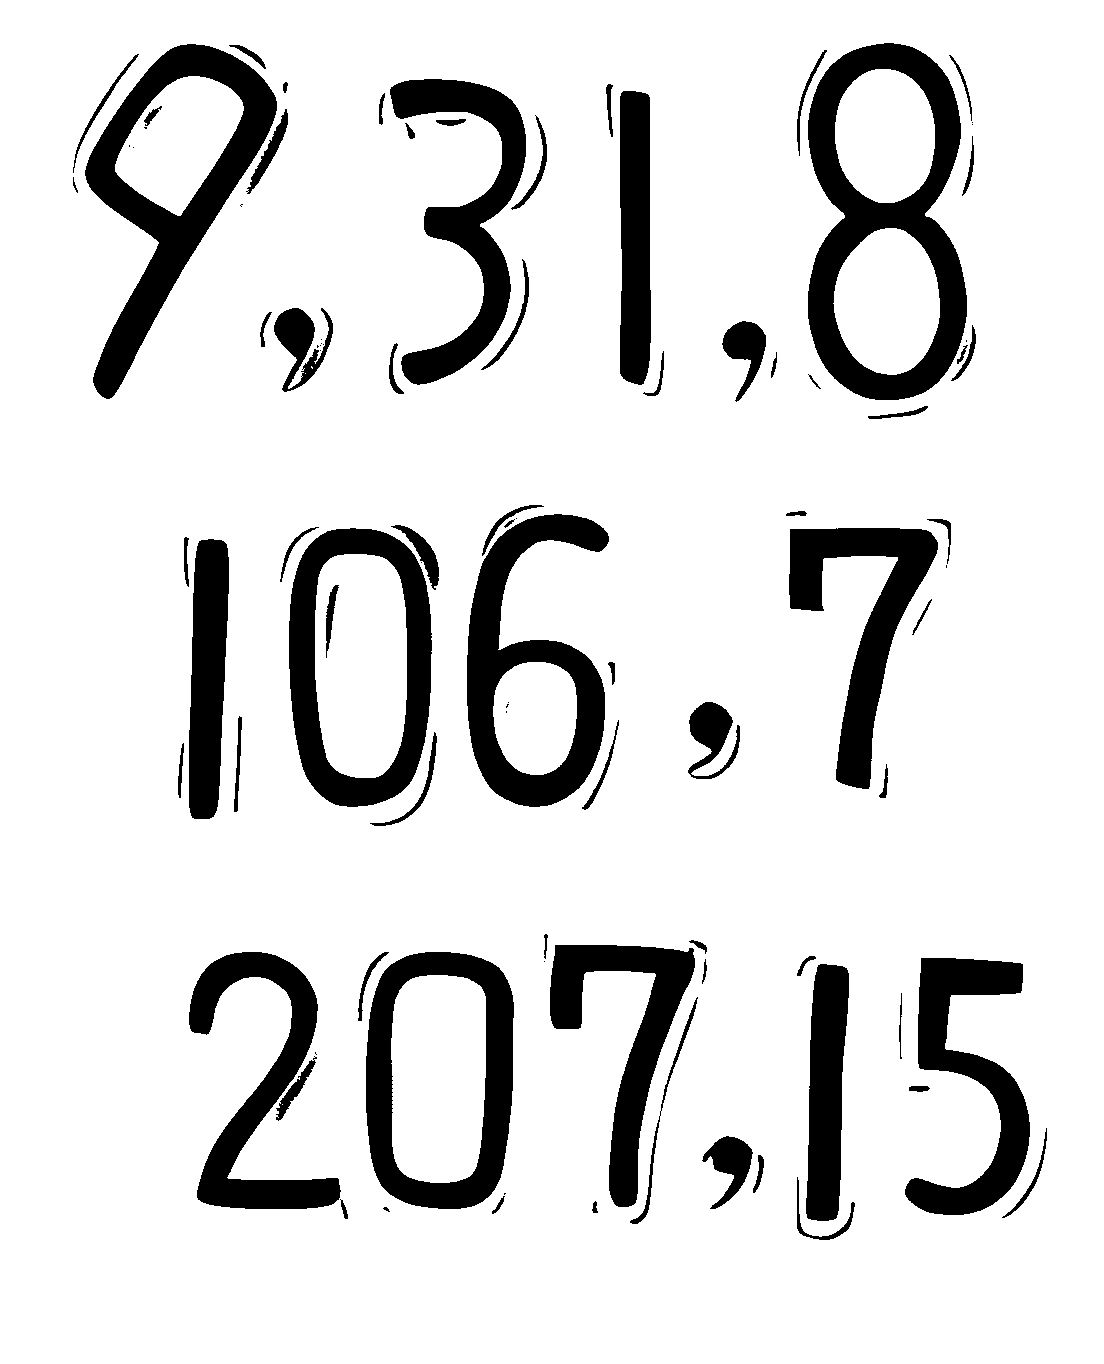
\includegraphics[width=1.1cm]{images/geral/image2.png}\\
\vspace{0.4cm}
\textit{J.}\\
% \vspace{1.2cm}

% ``\textit{Os valores das crianças que nunca conheceram a paz
% diferem dos valores das crianças que nunca conheceram a guerra!}''\\
% \vspace{0.4cm}
% \textit{Donquixote Doflamingo}
% \vspace{1.2cm}

% ``\textit{Mas não tenha medo. Este é o caminho que você escolheu. Comparado ao seu, nosso sofrimento terminará em um instante.}''\\
% \vspace{0.4cm}
% \textit{Fugaku}

\end{flushright}
		%
						%
\Resumo					%
Os ciclones extratropicais (ETCs) são sistemas recorrentes na costa do Atlântico Sul-Ocidental que geram ventos e precipitações, cuja coincidência espacial costuma ser assumida.
Enquanto o Hemisfério Norte conta com estudos sistemáticos sobre como esses campos se distribuem, no Hemisfério Sul é mais limitado o uso da densidade espacial e das Funções Ortogonais Empíricas (EOF) univariadas e multivariadas (MEOF) nas diferentes fases do desenvolvimento dos ETCs.
Esta tese desenvolve tal integração para avaliar se a intensidade dinâmica do ETC prediz a magnitude e a localização de seus máximos de vento a 10 metros e precipitação, ou se ambos os campos desenvolvem uma organização estrutural distinta segundo a fase evolutiva.

A análise se constrói sobre o catálogo de trajetórias por vorticidade relativa a 850~hPa \citep{gramcianinov2020analysis} e a classificação objetiva do ciclo de vida em quatro fases mediante \textit{CycloPhaser} \citep{coutodesouza2024new, deSouza2025CycloPhaser}, sobre o ERA5 (1979--2020).
A amostra foi estratificada por três regiões de ciclogênese (SBR, LPB, ARG) e dois estratos de intensidade: a População Global e o subconjunto dos ciclones mais intensos (p90, extraído da População Global).
Sobre essa base foram aplicadas, de forma progressiva, funções de densidade de probabilidade (PDF) de magnitude, estimação de densidade espacial (PDFe) de localização, decomposição EOF univariada com avaliação de significância mediante Bootstrap-$t$, e decomposição MEOF da covariância conjunta, integradas finalmente em protótipos estruturais.

Na População Global, um único modo EOF domina a variabilidade do vento (31--57\% da variância) e se correlaciona com a vorticidade; a precipitação, por sua vez, se distribui entre vários modos (EOF1 de apenas 11--16\%).
Essa organização muda no subconjunto p90. O vento se concentra no quadrante noroeste (moda de 23--25~m\,s$^{-1}$, densidades de até $27\times10^{-4}$ em SBR), enquanto, a partir da maturidade, os máximos de precipitação se afastam do centro e formam uma estrutura em arco a leste e sudeste.
Na População Global, o MEOF1 captura 14.8--26.6\% da covariância conjunta, com os gradientes de precipitação e vento em eixos perpendiculares. Em p90 cai para 11.65--23.47\% e, na maturidade, situa ambos os campos em setores opostos do ciclone, separação respaldada pela correlação significativa entre as PC1 univariadas de ambos os campos ($|r|$ entre $0.31$ e $0.45$), embora o vento domine esse modo conjunto na maioria dos casos.
Os protótipos estruturais quantificam essa separação em mais de $8^{\circ}$--$9^{\circ}$ durante a maturidade e o decaimento, com ARG alcançando a maior magnitude (${\sim}10$--$11^{\circ}$).
A magnitude dessa separação varia regionalmente sem um único fator identificado, embora sua direção, precipitação a leste-sudeste e vento a noroeste, se mantenha consistente nas três regiões.

Esses resultados mostram que, nos ETCs mais intensos do Atlântico Sul-Ocidental, os máximos de vento e precipitação se situam em quadrantes opostos durante a maturidade, e que a vorticidade do centro, que segue associada à organização do vento, deixa de descrever a da precipitação em SBR e LPB.
Esta tese combina PDFe, EOF univariado e MEOF para quantificar essa separação por fase e região de gênese no Atlântico Sul-Ocidental, com implicações para o risco costeiro no Brasil, Uruguai e Argentina.

\vspace{1cm}

\noindent \textbf{Palavras-chave:} América do Sul; ciclones extratropicais; vento a 10 metros; precipitação; estrutura espacial; EOF multivariada.
		%
						%
\Abstract					%
% ============================================================
%  ABSTRACT
% ============================================================
Extratropical cyclones (ETCs) are recurring systems along the Southwestern Atlantic coast that generate winds and precipitation, whose spatial coincidence is usually assumed.
While the Northern Hemisphere has systematic studies on how these fields are distributed, the use of spatial density estimation and of univariate and multivariate Empirical Orthogonal Functions (EOF and MEOF) across the different phases of ETC development is more limited in the Southern Hemisphere.
This thesis develops such an integration to assess whether ETC dynamic intensity predicts the magnitude and location of its 10-meter wind and precipitation maxima, or whether both fields develop a distinct structural organization depending on the evolutionary phase.

The analysis is built on a cyclone-tracking catalog based on 850-hPa relative vorticity \citep{gramcianinov2020analysis} and the objective classification of the life cycle into four phases using \textit{CycloPhaser} \citep{coutodesouza2024new, deSouza2025CycloPhaser}, applied to ERA5 (1979--2020).
The sample was stratified by three cyclogenesis regions (SBR, LPB, ARG) and two intensity strata: the Global Population and the subset of the most intense cyclones (p90, drawn from the Global Population).
On this basis, probability density functions (PDF) of magnitude, spatial density estimation (PDFe) of location, univariate EOF decomposition with significance assessed via Bootstrap-$t$, and MEOF decomposition of the joint covariance were applied progressively, ultimately integrated into structural prototypes.

In the Global Population, a single EOF mode dominates wind variability (31--57\% of variance) and is correlated with vorticity; precipitation, in contrast, is spread across several modes (EOF1 only 11--16\%).
This organization changes in the p90 subset. Wind concentrates in the northwest quadrant (mode of 23--25~m\,s$^{-1}$, densities up to $27\times10^{-4}$ in SBR), while, from maturity onward, precipitation maxima move away from the center and form an arc-shaped structure to the east and southeast.
In the Global Population, MEOF1 captures 14.8--26.6\% of the joint covariance, with precipitation and wind gradients along perpendicular axes. In p90 it drops to 11.65--23.47\% and, at maturity, places both fields in opposite sectors of the cyclone, a separation supported by the significant correlation between the univariate PC1 of both fields ($|r|$ between $0.31$ and $0.45$), although wind dominates this joint mode in most cases.
The structural prototypes quantify this separation at over $8^{\circ}$--$9^{\circ}$ during maturity and decay, with ARG reaching the largest magnitude (${\sim}10$--$11^{\circ}$).
The magnitude of this separation varies regionally without a single identified factor, although its direction, precipitation to the east-southeast and wind to the northwest, remains consistent across the three regions.

These results show that, in the most intense ETCs of the Southwestern Atlantic, wind and precipitation maxima lie in opposite quadrants at maturity, and that central vorticity, which remains associated with the organization of wind, no longer describes that of precipitation in SBR and LPB.
This thesis combines PDFe, univariate EOF, and MEOF to quantify this separation by phase and genesis region in the Southwestern Atlantic, with implications for coastal risk in Brazil, Uruguay, and Argentina.

\vspace{1cm}

\noindent \textbf{Keywords:} South America; extratropical cyclones; wind at 10 meters; precipitation; spatial structure; multivariate EOF.
		%
						%
\listoffigures 				% lista de figuras (opcional)
\listoftables 				% lista de tabelas (opcional)
\tableofcontents 			% sumário
						%
\cleardoublepage			%
\pagestyle{fancy}			% formatação para corpo do texto
						%
\chapter{Introdução} \label{ch:introduccion}

% ============================================================
%  BLOCO 1 — CONTEXTO: RELEVÂNCIA DO FENÔMENO E ESTADO DA ARTE
% ============================================================

% --- 1.1: Papel climático e dinâmico global; algoritmos de rastreamento ---
Os ciclones extratropicais (ETC, sigla em inglês) são sistemas sinóticos recorrentes em latitudes médias e altas que dominam o tempo severo dessas regiões.
\citet{hoskins2005new} caracterizam os \textit{storm tracks} do HS, os corredores preferenciais por onde se concentra a atividade ciclônica do hemisfério.
Para sua quantificação, foram desenvolvidos algoritmos de rastreamento objetivo, como propõe \citet{sinclair1994objective}, utilizando a vorticidade relativa para identificá-los e rastreá-los independentemente do fluxo de fundo, enquanto \citet{simmonds1999southern} desenvolveram um esquema complementar, usando a pressão ao nível do mar, para o rastreamento automático de sistemas no HS; e trabalhos atuais como o de \citet{padilhareinke2024objective} continuam optando pela abordagem de vorticidade relativa para a região.

% --- 1.2: Estado da arte regional — climatologia, diversidade estrutural e regionalização ---
Inicialmente, autores como \citet{gan1991surface} quantificaram que a ciclogênese na região sul-americana é mais frequente no inverno e que sua variabilidade interanual repercute na precipitação do sul do Brasil.
Pouco depois, a climatologia hemisférica de \citet{jones1993climatology} confirmou esse sinal, identificando a região sul-americana como um núcleo de densidade ciclônica próprio das latitudes extratropicais, distinto das concentrações maiores em latitudes próximas ao polo.
No Atlântico Sul ocidental, essa atividade ciclônica é particularmente intensa, sendo os ciclones extratropicais os sistemas mais frequentes da região \citep{reboita2026meteorology}.
Diversos estudos, como o de \citet{reboita2010south}, construíram uma climatologia para o Atlântico Sul e identificaram três centros preferenciais de ciclogênese: um ao sul, vinculado à instabilidade baroclínica dos ventos de oeste, e dois mais ao norte, próximos ao Uruguai e ao sul do Brasil.
Trabalhos posteriores refinaram essa climatologia por meio de comparações entre reanálises \citep{gramcianinov2020analysis} e da caracterização de sua variabilidade interanual \citep{padilhareinke2026characterization}.
No entanto, essa atividade ciclônica não é dinamicamente uniforme. \citet{hart2003cyclone} demonstrou que os sistemas transitam ao longo de um contínuo estrutural, e não de categorias estáticas, e no Atlântico Sul essa heterogeneidade se manifesta em ciclones de estrutura térmica híbrida \citep{evans2012climatology} e em sistemas que seguem o modelo de Shapiro-Keyser, com fratura da frente fria e seclusão quente na maturidade \citep{gozzo2013air}.
Essa diversidade regional também responde à Cordilheira dos Andes, cujo forçante orográfico aumenta a baroclinicidade a sotavento \citep{gan1994influence}, que, combinada com os gradientes de temperatura superficial do mar \citep{reboita2026meteorology}, consolida focos de atividade ciclogenética diferenciados na costa leste da América do Sul, cujos mecanismos são desenvolvidos na Seção~\ref{sec:tb_regiones} dos Fundamentos.
\label{sec:definicion_regiones}%
Pelo exposto, este estudo se concentra em três regiões de ciclogênese documentadas por diversos autores \citep{crespo2020potential, gramcianinov2019properties, reboita2026meteorology} e delimitadas seguindo a proposta de \citet{gramcianinov2019properties}: o Sul-Sudeste do Brasil (\textit{Southeast Brazil}, SBR), a bacia de drenagem do Rio da Prata (\textit{La Plata Basin}, LPB) e a costa sudeste da Argentina (\textit{Argentina}, ARG).

% --- 1.3: Mecanismos dinâmicos internos já estabelecidos ---
A leste dos Andes, a convergência de vento em níveis baixos favorece as condições que produzem precipitações intensas no sudeste da América do Sul, cuja liberação de calor latente retroalimenta e reforça a intensificação do sistema \citep{vera2002cold}.
O transporte meridional de umidade dos trópicos até esses sistemas é mediado pelo Jato de Baixos Níveis da América do Sul \citep{reboita2026meteorology}, enquanto os fluxos turbulentos de calor superficiais oceano-atmosfera, como aponta \citet{reboita2022from}, não apenas desestabilizam a atmosfera, mas também atuam como fonte diabática que reforça a intensidade do sistema.
Essa advecção quente se organiza em torno de estruturas de mesoescala conhecidas como cintas transportadoras, a Cinta Transportadora Quente e a Cinta Transportadora Fria (WCB e CCB, respectivamente), cujo papel na distribuição espacial de vento e precipitação é desenvolvido na Seção~\ref{subsec:tb_modelos}.
O vento em superfície e a precipitação são, por isso, as variáveis escolhidas para caracterizar esses impactos, conforme detalhado na Seção~\ref{sec:tb_compound_def}.

% ============================================================
%  BLOCO 2 — PROBLEMA: A LACUNA NA CARACTERIZAÇÃO ESTRUTURAL
% ============================================================
Apesar desse conhecimento consolidado sobre onde, quando e por qual mecanismo se formam os ETC do Atlântico Sul, persistem lacunas sobre \emph{como} se distribuem espacialmente as magnitudes de superfície ao longo do ciclo de vida.
Esse desconhecimento reside, em parte, no fato de que a intensidade de um ETC não pode ser capturada por uma única métrica. \citet{corner2025classification} mostram que, embora as medidas dinâmicas como a vorticidade, a pressão e o vento em superfície se relacionem linearmente entre si, seu vínculo com a precipitação e a severidade dos ventos é consideravelmente mais fraco e não linear, e \citet{sinclair2023relationship} confirmam esse limite ao advertir que um ETC pode ser dinamicamente intenso, mas gerar pouca chuva se não houver suprimento adequado de umidade.
A essa insuficiência escalar soma-se uma insuficiência posicional.
Os máximos de vento não se distribuem uniformemente em torno do centro do ciclone, mas se concentram em quadrantes específicos cuja localização varia com estruturas de mesoescala e com a fase de seu desenvolvimento \citep{eisenstein2023identification}, mecanismo desenvolvido na Seção~\ref{subsec:tb_kde_asimetria}.

Os ETCs podem se desenvolver por meio de mecanismos atípicos para a região, como constataram \citet{gozzo2013air,reboita2022from}, o que impede assumir seus campos de superfície a priori.
Embora vento e precipitação respondam a mecanismos distintos, \citet{chen2025characteristics} quantificam que a maioria dos extremos de vento e precipitação associados a ETC coocorrem, demandando uma análise conjunta de sua covariabilidade estrutural ao longo do ciclo de vida.
Nessa mesma linha, \citet{han2025system} propõem um referencial de classificação que vincula a evolução do sistema a suas manifestações de vento e precipitação, superando a limitação de abordagens centradas apenas na estrutura térmica, necessidade reforçada por campanhas aerotransportadas que caracterizam camadas de convecção interna não capturadas por produtos convencionais de menor resolução \citep{kaylee2025convection}.
Essa caracterização tem sido limitada pela resolução espacial disponível. \citet{priestley2022improved} mostram que modelos de baixa resolução subestimam ventos extremos por não resolverem as mesoescalas, enquanto \citet{neu2013intercomparison} apontam que a variabilidade na forma e no tamanho dos ETCs gera divergências de detecção, especialmente em topografia complexa.

% ============================================================
%  BLOCO 3 — JUSTIFICATIVA E IMPLICAÇÕES
% ============================================================
No Atlântico Sul ocidental, os ETCs modulam o estado do mar costeiro \citep{gramcianinov2023impact}, com variabilidade intrassazonal (~40 dias) \citep{sasaki2021intraseasonal}, sugerindo que o risco costeiro pode ser modulado em escalas que excedem eventos sinóticos individuais.
Os registros de 40 anos mostram tendência a ciclones maiores e mais intensos no HS \citep{simmonds2000variability}, intensificação que projeções de aquecimento projetam particularmente na precipitação (~7\%/K) \citep{kodama2019perspective}, e que simulações de alta resolução também antecipam para o setor quente dos ETC mais intensos, com aumentos significativos de vento e precipitação durante suas etapas de desenvolvimento \citep{gentile2025response}.
No litoral sul do Brasil, \citet{bartolomei2024extremos} documentam impactos socioeconômicos de ETCs invernais, confirmados como os principais motores de tempestades costeiras \citep{miranda2026patterns,bitencourt2010relating}.
Caracterizar onde e em qual fase do ciclo se concentram os máximos de vento e precipitação, em vez de depender de métricas escalares, permitiria antecipar impactos costeiros com maior precisão e construir referenciais de classificação que vinculem a evolução do sistema a manifestações de superfície \citep{han2025system}.

A viabilidade dessa caracterização se apoia em três desenvolvimentos recentes.
Primeiro, a disponibilidade da reanálise ERA5 \citep{hersbach2020era5}, cujo espaçamento horizontal ($\sim$31 km) e temporal (horário) permite resolver os gradientes de pressão e os fluxos de umidade que gerações anteriores de dados suavizavam; validações específicas para a região \citep{gramcianinov2020analysis} e comparações com outras fontes de dados para a detecção de ciclogênese na América do Sul \citep{dalanhese2023new} respaldam essa escolha, embora o ERA5 apresente vieses conhecidos na representação dos extremos mais intensos, discutidos na Seção~\ref{sec:datos_era5}.
Segundo, a base de dados de trajetórias de \citet{gramcianinov2020analysis}, fundamentada no rastreamento por vorticidade relativa a 850 hPa ($\zeta_{850}$) em vez da pressão ao nível do mar, cuja sustentação é desenvolvida na Seção~\ref{sec:tb_vorticidad}, e que além disso incorpora a segmentação objetiva do algoritmo \textit{CycloPhaser} \citep{coutodesouza2024new, deSouza2025CycloPhaser}, que define quatro fases dinâmicas discretas, incipiente, intensificação, maturidade e decaimento, e supera as limitações das classificações clássicas no contexto do Atlântico Sul \citep{deSouza2025CycloPhaser}, em sintonia com o referencial oferecido pelo modelo Shapiro-Keyser \citep{shapiro1990life,shapiro1999bridge} para interpretar a distribuição espacial dos máximos de vento e precipitação (Seção~\ref{subsec:tb_modelos}).
Terceiro, a disponibilidade de técnicas estatísticas capazes de capturar simultaneamente a assimetria estrutural de cada campo e sua covariabilidade.
Dado que a estrutura do ciclone apresenta uma variabilidade espacial contínua na qual a circulação do vento e os núcleos de precipitação podem covariar durante a evolução do sistema, a análise de Funções Ortogonais Empíricas Multivariadas (MEOF) permite extrair modos de variabilidade conjunta de variáveis fisicamente distintas \citep{liang2018multivariate}, diferentemente da análise univariada de EOF aplicada separadamente a cada campo, capturando assim a organização espacial conjunta de ambos.
A utilidade desses padrões e de suas componentes principais transcende a caracterização descritiva, com aplicação prática inclusive na previsão de precipitação \citep{sun2022evaluation}, e sua robustez estatística pode ser avaliada mediante técnicas de reamostragem (\textit{bootstrap}) que distinguem os sinais físicos consistentes do ruído de amostragem próprio de cada subconjunto.

% ============================================================
%  BLOCO 4 — PERGUNTA DE PESQUISA, HIPÓTESE E OBJETIVO
% ============================================================

Os dados de ERA5, a detecção dinâmica por $\zeta_{850}$ \citep{gramcianinov2020analysis} e a classificação objetiva de fases mediante \textit{CycloPhaser} \citep{coutodesouza2024new, deSouza2025CycloPhaser}, juntamente com a análise univariada (EOF) e multivariada (MEOF) desenvolvida nesta investigação, constituem a base para quantificar a evolução da estrutura espacial dos campos de vento e precipitação na região, e para construir, a partir das fases previamente classificadas, protótipos estruturais que sintetizem as características típicas dos ETCs para cada região de gênese e fase evolutiva.
Com esse referencial de dados, detecção dinâmica e ferramentas analíticas, propõe-se a pergunta que guia esta investigação: como evolui espacialmente a distribuição de vento e precipitação nos ETC do Atlântico Sul, e quais configurações caracterizam essa organização durante as fases incipiente, intensificação, maturidade e decaimento?
Postula-se que os campos de vento e precipitação apresentam padrões de assimetria que variam entre fases evolutivas, entre regiões de gênese e entre estratos de intensidade dinâmica, contrastando a População Global de ciclones com o subconjunto p90, e que tais padrões não são capturáveis mediante métricas escalares de intensidade central.

\section{Objetivos do Projeto de Pesquisa}

\subsection{Objetivo Geral}
Caracterizar a evolução da estrutura espacial do vento a 10 metros e da precipitação durante as fases do ciclo de vida dos ETC do Atlântico Sul, por meio de seus padrões de variabilidade e da densidade probabilística de seus máximos, estratificando por região de gênese e por intensidade dinâmica (População Global e subconjunto p90).

\subsection{Objetivos Específicos}
\begin{enumerate}
    \item Consolidar uma base de dados semilagrangeana dos ETC do Atlântico Sul que associe os campos horários de alta resolução de vento e precipitação (ERA5) às trajetórias e fases dinâmicas (incipiente, intensificação, maturidade e decaimento), estratificando a amostra resultante por região de gênese (SBR, LPB e ARG) e por intensidade dinâmica.

    \item Quantificar a distribuição estatística e a assimetria espacial dos máximos de vento a 10 m e de precipitação mediante estimação de densidade por núcleos, caracterizando tanto a distribuição de probabilidade de suas magnitudes (PDF unidimensional) quanto a localização preferencial desses máximos em relação ao centro do ciclone (PDF espacial).

    \item Identificar os modos dominantes de variabilidade espacial dos campos de vento e precipitação mediante Funções Ortogonais Empíricas univariadas (EOF) e multivariadas (MEOF), avaliando o padrão estrutural individual de cada variável e sua covariabilidade conjunta.

    \item Construir protótipos estruturais sintéticos por fase evolutiva e região de gênese, integrando os padrões EOF1 univariados de cada campo com as densidades probabilísticas de localização de máximos (PDFe), para caracterizar a organização espacial conjunta dos máximos de vento e precipitação.
\end{enumerate}
		%
\chapter{Fundamentos teóricos}\label{ch:theoretical_background}

% ============================================================
%  BLOCO A — CONTEXTO DINÂMICO
% ============================================================

\section{Ciclones extratropicais no Atlântico Sul}\label{sec:tb_fundamentos}

A teoria clássica, desenvolvida a partir dos primeiros estudos sinóticos de ciclones de latitudes médias, definiu-os como vórtices de núcleo frio que evoluem a partir de uma onda sobre uma frente de discontinuidade térmica entre massas de ar frio e quente \citep{bjerknes1922life}.
Esse modelo foi revisado décadas depois por \citet{shapiro1990life}, cujo referencial estrutural é desenvolvido na Seção~\ref{subsec:tb_modelos}.
No Hemisfério Sul, \citet{hoskins2005new} geraram a climatologia e confirmaram a concentração da ciclogênese nas zonas baroclínicas.
No Atlântico Sul, \citet{sinclair1995climatology} destacou que a ciclogênese é influenciada pelos gradientes térmicos oceânicos e pela orografia, enquanto \citet{inatsu2004zonal} demonstraram que a assimetria zonal do \textit{storm track} é organizada por ondas estacionárias troposféricas, moduladas regionalmente pela topografia dos Andes, cuja interação com o fluxo de níveis baixos também favorece a propagação de ondas baroclínicas sobre a América do Sul \citep{vera2002cold}.
Embora a instabilidade baroclínica proporcione o ambiente favorável para a gênese, processos diabáticos associados à liberação de calor latente modulam a evolução e a intensidade do sistema, como concluiu \citet{coutodesouza2024thesis}.
Isso concorda com experimentos de sensibilidade numérica de \citet{reboita2022from}, nos quais a supressão dos fluxos de calor sensível e latente alterou a estrutura térmica e a intensidade do vórtice, efeito também relatado por \citet{gozzo2013air}.

% ============================================================
%  BLOCO B — DETECÇÃO E RASTREAMENTO
% ============================================================
\section{Detecção de ETC}\label{sec:tb_vorticidad}

\subsection{Referencial semilagrangeano}\label{subsec:tb_lagrangiano}
A variabilidade estrutural dos ETCs do Atlântico Sul requer um referencial comum que não dilua o sinal em médias geográficas nem incorpore ruído de sistemas adjacentes.
A abordagem euleriana superpõe campos de variáveis, dificultando a observação de assimetrias estruturais durante a evolução.
A abordagem semilagrangeana evita essa diluição centrando cada ETC em seu núcleo ciclônico com coordenadas relativas $(\Delta x, \Delta y)$, preservando a organização espacial e isolando seu sinal dentro de um domínio que se desloca com a trajetória.
Um domínio de $20^{\circ} \times 20^{\circ}$ foi empregado no Atlântico Sul-Ocidental por \citet{cardoso2022synoptic}.
Essa abordagem lagrangiana demonstrou utilidade em escala global: \citet{laurila2021characteristics} mostram que ela permite construir composites no Hemisfério Norte, enquanto \citet{priestley2022improved} a aplicaram em ambos os hemisférios para quantificar a estrutura e a intensidade dos ventos, \citet{pepler2020dimensional} a empregaram com um raio de $10^{\circ}$ no sudeste da Austrália para estudar a severidade de ventos e chuva, e \citet{dacre2012atlas} a utilizaram com um raio de $20^{\circ}$ no Atlântico Norte para construir um atlas de compostos que documenta sistematicamente a estrutura e a evolução do ciclone.

\subsection{Vorticidade relativa em 850 hPa}\label{subsec:tb_zeta}
Na abordagem de rastreamento semilagrangeano, a vorticidade relativa em 850 hPa ($\zeta_{850}$) se estabeleceu como a variável para identificar e rastrear ciclones extratropicais.
No Hemisfério Sul (HS), esses sistemas se desenvolvem imersos em um fluxo zonal de oeste que os desloca com rapidez; por isso, em suas etapas iniciais a queda de pressão costuma ficar mascarada, apresentando-se como cavados abertos em vez de centros fechados \citep{sinclair1994objective}, o que torna a pressão ao nível do mar (MSLP) uma métrica inadequada na detecção precoce.
Para resolver esse problema, \citet{sinclair1997objective} recomendaram utilizar a vorticidade relativa em níveis baixos em vez da pressão ao nível do mar; nesta tese adota-se especificamente $\zeta_{850}$.
Essa variável tem sido usada objetivamente em climatologias de todo o HS \citep{padilhareinke2024objective} e em estudos regionais do Atlântico Sul \citep{gramcianinov2019properties}, além do HN por \citet{corner2025classification}, e na segmentação objetiva do ciclo de vida por \citet{coutodesouza2024new}, que emprega $\zeta_{850}$ como variável base para delimitar as quatro fases mediante detecção de picos e vales em sua série temporal.

\begin{equation}\label{eq:vorticidad_relativa}
\zeta = \mathbf{k} \cdot (\nabla \times \mathbf{V}) = \frac{\partial v}{\partial x} - \frac{\partial u}{\partial y},
\end{equation}

\noindent em que $u$ e $v$ são as componentes zonal e meridional do vento horizontal, respectivamente.
A 850 hPa, $\zeta$ filtra o fluxo zonal de translação e captura a rotação ciclônica intrínseca induzida por forçantes de mesoescala \citep{hoskins2005new}, sinal que precede a manifestação no campo de pressão durante as etapas iniciais \citep{sinclair1994objective}, critério adotado como base de detecção nos principais algoritmos de rastreamento e bases de dados objetivas.

\subsection{Estratificação}\label{subsec:tb_poblaciones}
A intensidade dinâmica é quantificada mediante o mínimo de vorticidade relativa alcançado durante a trajetória completa, $\zeta_{850}^{\min}$.
Essa estratificação se justifica mediante \citet{priestley2022improved}, que selecionaram os 10\% de ciclones com maior vorticidade ciclônica em seu pico de intensidade.
A pertinência dessa estratificação, independentemente da métrica de intensidade empregada, encontra respaldo adicional em \citet{andrade2024composite}, que mostram que categorias com maior taxa de aprofundamento exibem comportamento estrutural coerente e diferenciado, com maiores fluxos de calor superficiais.
Isso sugere que os sistemas mais intensos, seja em termos de vorticidade ou de pressão, apresentam uma organização física distintiva que justifica tratá-los como subconjunto separado.
Adota-se um critério percentílico ($p90$) para isolar os sistemas mais intensos.
No HS, onde a vorticidade ciclônica é negativa, selecionar p90 em valor absoluto equivale ao $\zeta_{850}^{\min}$ mais negativo, ou seja, o mais intenso.
Para garantir comparabilidade estrutural, a homogeneidade evolutiva requer ciclo de vida completo, entendido como a sequência de quatro fases evolutivas (Seção~\ref{subsec:tb_fases}), sem reintensificações que introduzam ruído.
Esse critério retém entre 43\% e 52\% dos sistemas por região (Tabela~\ref{tab:conteo_ciclones}), a partir de uma versão atualizada do catálogo de trajetórias de \citet{gramcianinov2020analysis}, com as fases classificadas mediante \textit{CycloPhaser} \citep{coutodesouza2024new, deSouza2025CycloPhaser}.
Os filtros específicos são detalhados na Seção~\ref{sec:poblaciones_estudio}.
Do exposto emergem dois estratos de análise complementares:
\begin{itemize}
\item População Global: conjunto de referência integrado por ciclones de ciclo de vida completo que representam o comportamento médio.
\item Subconjunto p90: estrato de alta intensidade dinâmica extraído do percentil superior do valor absoluto de $\zeta_{850}^{\min}$ dentro da População Global (PG).
\end{itemize}
Essa estratificação dupla busca responder se uma maior intensidade do vórtice se associa a mudanças sistemáticas na organização espacial em superfície.
Os sistemas $p90$ mantêm uma evolução temporal coerente com a PG, alcançando sua intensidade máxima predominantemente durante a fase de maturidade (Tabela~\ref{tab:fase_max_intensidad}).

% ============================================================
%  BLOCO C — REGIÕES DE CICLOGÊNESE
% ============================================================

\section{Regiões de ciclogênese}\label{sec:tb_regiones}
No Atlântico Sul-Ocidental, \citet{gramcianinov2019properties} constataram que a interação entre o fluxo de oeste, a topografia dos Andes \citep{gan1994influence} e a Temperatura Superficial do Mar define três regiões de gênese com características físicas diferenciadas, delimitação que \citet{reboita2010south} já havia estabelecido previamente, empregando também a vorticidade relativa (ainda que em outro nível atmosférico) para identificar esses focos na América do Sul.

\subsection{Sul-sudeste do Brasil (SBR)}\label{subsec:tb_sbr}
A região SBR constitui um dos centros de ação preferenciais para a ciclogênese extratropical no litoral brasileiro.
Os ciclones podem se iniciar por instabilidade baroclínica associada à advecção de ar quente em níveis baixos e um cavado em níveis médios-altos \citep{gozzo2014subtropical}, mas sua intensificação é fortemente modulada pelos fluxos turbulentos de calor sensível e latente na camada limite \citep{gozzo2013air}, que organizam a convergência de umidade e intensificam o sistema em seu setor quente.
A análise energética de \citet{coutodesouza2024thesis} mostrou que a contribuição diabática para a energia do sistema em SBR se eleva durante o inverno, diferentemente de ARG, onde essa contribuição é a menor das três regiões.
\citet{gramcianinov2024early} demonstraram ainda que, durante a ciclogênese inicial em SBR, os modelos de alta resolução conseguem representar as estruturas de mesoescala de advecção quente e convergência de umidade em camadas baixas.

\subsection{Bacia do Rio da Prata (LPB)}\label{subsec:tb_lpb}
Na região de LPB, \citet{gramcianinov2024early} destacaram que a ciclogênese é favorecida pela interação entre a Alta Subtropical do Atlântico Sul e o Jato de Baixos Níveis da América do Sul, que intensifica o transporte de umidade em direção ao sistema, e que a convergência de umidade em camadas baixas constitui o mecanismo dominante de intensificação.
\citet{coutodesouza2024thesis} constatou que também depende do transporte de umidade do Jato de Baixos Níveis da América do Sul sobre o flanco oriental dos Andes e do Anticiclone Subtropical do Atlântico Sul em direção à costa sudeste, o que se traduz na maior contribuição diabática para a energia do sistema entre as três regiões.
Em linha com esse forçante de umidade, \citet{reboita2010south} mostraram que a região se caracteriza por uma alta frequência de sistemas ciclônicos e por sua interação com o transporte de umidade desde latitudes tropicais, padrão que \citet{laureanti2024relation} também documentam, mediante compostos próprios, para o centro-leste do Brasil, onde o deslocamento para o norte do SALLJ coincide com uma circulação ciclônica anômala de níveis baixos que intensifica o transporte de umidade amazônica.

\subsection{Argentina (ARG)}\label{subsec:tb_arg}
O setor mais austral responde a um regime dinâmico dominado pela baroclinicidade de grande escala, diferentemente do forçamento termodinâmico de superfície que caracteriza SBR e LPB.
\citet{hoskins2005new} mostraram que a ciclogênese nessa faixa se concentra a leste dos Andes, padrão que \citet{coutodesouza2024thesis} corroborou empiricamente em sua própria climatologia de trajetórias para a região.
\citet{sinclair1995climatology} mostra que a ciclogênese ao largo da costa da Argentina ocorre durante todo o ano, diferentemente de outras zonas de gênese a sotavento cuja atividade depende de gradientes térmicos oceânicos sazonais.
\citet{mendes2010climatology} identificaram nessa região um agrupamento de trajetórias (\textit{storm-track}) próprio dentro do setor sul-americano.
% ============================================================
%  BLOCO D — ESTRUTURA INTERNA
% ============================================================

\section{Estrutura interna}\label{sec:tb_evolucion}

\subsection{Modelo conceitual de estrutura interna}\label{subsec:tb_modelos}

Os ciclones extratropicais intensos do Atlântico Sul costumam seguir o modelo Shapiro-Keyser proposto por \citet{shapiro1990life}, caracterizado por quatro traços diagnósticos: a fratura da frente fria (\textit{frontal fracture}), a frente curvada (\textit{bent-back front}), a estrutura em T (\textit{T-bone}) e o isolamento de uma massa de ar quente no núcleo (\textit{warm seclusion}).
Esse modelo captura a forma que o sistema adota, mas é o modelo de cintas transportadoras que explica como essa forma se traduz na distribuição de vento e precipitação em superfície.
O WCB, definido originalmente como a corrente ascendente de ar quente e úmido que se origina no setor quente \citep{carlson1980airflow}, e seu respectivo jato de baixo nível se organizam em torno do vórtice \citep{browning1986conceptual}, e a ascensão e o giro anticiclônico desse fluxo quente modulam as estruturas de mesoescala, concentrando as bandas de precipitação adiante da frente fria \citep{coll2024lagrangian}.
O WCB se origina no lado \textit{equatorward} do centro e ascende sobre a frente quente, enquanto o CCB (frio e denso) ocupa o lado \textit{poleward} \citep{dacre2023climatology}.
Essa organização frontal do WCB é o que vincula sua posição aos máximos de precipitação \citep{catto2015fronts}.

Sob uma simetria especular em relação ao equador, essa organização deveria se inverter apenas no eixo norte-sul ao passar para o HS, onde o sentido de giro ciclônico é horário em vez de anti-horário, enquanto a disposição leste-oeste deveria se manter.
No HN, o jato do WCB domina o quadrante sudeste (nordeste no HS) e afeta ali a maior área do composto, ainda que com os ventos mais fracos em média; os ventos mais intensos se concentram no setor frio \citep{eisenstein2023identification}. Essa localização do WCB é consistente com o modelo Shapiro-Keyser \citep{catto2010climate}, enquanto o fluxo do setor quente resulta sistematicamente mais fraco no HS do que no Hemisfério Norte \citep{hodges2011comparison}.
A conexão dinâmica entre WCB e CCB explica essa assimetria de vento e precipitação: o CCB ganha vorticidade potencial ao deslocar-se pelo lado frio da frente curvada, sob a região de máxima liberação de calor latente do WCB ascendente, o que localiza o jato de baixo nível mais intenso na extremidade da frente curvada \citep{schemm2014linkage}, padrão confirmado em ambos os hemisférios \citep{priestley2022improved} e documentado em um caso real do Japão, onde a banda de precipitação estratiforme se estendeu a leste do centro sobre o CCB \citep{sawada2021heavy}.

Uma intrusão seca (DI) descendo sobre o WCB pode gerar um terceiro máximo de precipitação, de caráter convectivo e localizado próximo ao centro do ETC, distinto da banda estratiforme oriental já descrita \citep{sawada2021heavy}.
Durante a oclusão, uma corrente conhecida como \textit{trowal} (\textit{trough of warm air aloft}), que ascende ciclonicamente dentro do quadrante ocluído, reorganiza a precipitação em uma banda periférica arqueada, intensificada pelo forçante adicional de ascensão frontal \citep{naud2025lifecycle}, que já não coincide com o núcleo de vento, padrão documentado no HN \citep{martin1999forcing}.
O \textit{Sting Jet} (SJ), estrutura de mesoescala do modelo Shapiro-Keyser, desce de níveis médios dentro dessa mesma intrusão seca, acima do CCB, produzindo os ventos mais intensos na zona de fratura frontal, distinta do WCB e do CCB, segundo casos documentados no HN \citep{clark2005sting, clark2018sting, martinez2014cold}.

\subsection{Assimetria espacial das variáveis}\label{subsec:tb_kde_asimetria}

As estruturas descritas na seção anterior (WCB, CCB, intrusão seca e \textit{sting jet}) ocupam setores distintos em torno do centro, de modo que o vento e a precipitação em superfície não se distribuem simetricamente ao seu redor.
Cada variável concentra seus máximos em quadrantes preferenciais, que não coincidem necessariamente entre si e que se deslocam ao longo do ciclo de vida.

Na precipitação, essa assimetria adota a forma de vírgula associada ao WCB.
Em compostos que combinam ambos os hemisférios, o máximo se localiza em direção ao polo e a leste do centro (sudeste no HS) e se prolonga em forma de vírgula, enquanto a oeste, no setor frio, a precipitação é mínima e intermitente \citep{naud2020evaluation}; \citet{field2007precipitation}, cuja análise de ciclones oceânicos inclui o Atlântico Sul, descreveram a mesma vírgula a leste do centro.
\citet{mcerlich2023extremes}, com compostos de ERA5 para todo o HS, mostraram que a precipitação se agrupa em torno do centro e se prolonga em uma cauda que gira em sentido horário conforme o ETC evolui, e que, quanto maior o limiar de intensidade, mais ela se restringe à região do WCB.
Ali podem se formar núcleos de convecção embebida que, em um caso documentado, produziram precipitação local superior a 6~mm em 15~min \citep{oertel2021warm}.
A inversão entre hemisférios, no entanto, não explica as diferenças de magnitude. \citet{kodama2019perspective} mostraram que os ETCs oceânicos intensos do HS precipitam, em média, menos que os do HN (7.7 contra 10.7~mm/dia em um raio de 550~km, segundo um de seus conjuntos de dados), diferença que atribuem à menor umidade disponível.
Nessa linha, os experimentos numéricos de \citet{gozzo2013air} no Atlântico Sul mostraram que os fluxos turbulentos de calor sensível e latente condicionam a extensão da precipitação, e que, com esses fluxos, na maturidade, ela se distribui em torno do centro, ao longo da frente quente e adiante da frente fria.

No vento, segundo \citet{catto2016extratropical}, os máximos se concentram em três núcleos espacialmente distintos, associados ao WCB, ao CCB e ao \textit{sting jet} (Seção~\ref{subsec:tb_modelos}), cada um característico de um momento distinto do ciclo de vida em relação ao instante de máxima profundidade e à evolução frontal, diferenciação que \citet{eisenstein2023identification} também observaram em uma climatologia europeia, onde as características de mesoescala associadas aos ventos mais intensos diferem em sua localização relativa ao centro e em seu momento de ocorrência.
No Atlântico Norte, os compostos centrados no ciclone de \citet{rudeva2011composite} situam o máximo de vento ao sul do centro (lado equatorial no HN) e mostram que ele se intensifica de 8--9 para 14--16~m/s durante o aprofundamento, e quanto aos extremos, \citet{gentile2023observed} mostraram, com estações marítimas do Mar do Norte, que os eventos do setor frio (associados ao CCB) são entre 1.5 e 3 vezes mais frequentes que os do setor quente (WCB), conforme o limiar de intensidade considerado.
No Atlântico Sul, durante as primeiras etapas do ciclone, \citet{gramcianinov2024early} associaram a advecção quente a leste do centro em SBR e LPB a ventos intensos de noroeste, originados em LPB pela combinação do Anticiclone Subtropical do Atlântico Sul e o Jato de Baixos Níveis da América do Sul no quadrante nordeste.

Essa dependência setorial e de fase se soma ao fato de que, como apontam \citet{corner2025classification}, nenhuma métrica única resume a intensidade de um ETC.
Por isso, nesta tese os campos são analisados em coordenadas relativas ao centro e particionados por fase (Seções~\ref{subsec:tb_compositing} e~\ref{subsec:tb_fases}), e a posição de seus máximos é tratada como uma distribuição (Seção~\ref{subsec:tb_kde}).

\subsection{Fases do ciclo de vida}\label{subsec:tb_fases}
Para caracterizar a evolução temporal do vento e da precipitação, aqui se emprega a segmentação do ciclo de vida em quatro fases discretas incluída na base de trajetórias (Seção~\ref{sec:bd_ciclones}) e obtida com \textit{CycloPhaser} \citep{deSouza2025CycloPhaser} segundo \citet{coutodesouza2024new}.
Essa ferramenta identifica as fases a partir da série temporal de $\zeta_{850}$ e de sua derivada, a mesma variável com que os ciclones foram detectados (Seção~\ref{subsec:tb_zeta}), o que mantém a coerência entre o critério de detecção e o de segmentação.
Embora o algoritmo atribua limites precisos a cada fase, a estrutura do ciclone muda de forma gradual, e os instantes próximos a uma transição conservam traços da fase anterior ou anticipam os da seguinte.
Por isso, nesta tese cada fase é representada unicamente por seus instantes centrais, onde a configuração dos campos de superfície própria dessa fase se expressa com maior clareza (Seção~\ref{sec:procesamiento_lagrangiano}).

\begin{enumerate}
    \item \textit{Incipiente:} Corresponde ao surgimento inicial de uma circulação ciclônica organizada.
    No contexto regional, essa fase costuma ser associada à interação entre um cavado em altitude e forçantes de superfície, como a orografia dos Andes ou gradientes térmicos costeiros.

    \item \textit{Intensificação:} Período caracterizado pelo rápido crescimento da vorticidade ciclônica.
    Essa etapa é impulsionada por uma retroalimentação entre a instabilidade dinâmica e os fluxos de calor latente e sensível.

    \item \textit{Maturidade:} Etapa em que o sistema alcança sua intensidade máxima (pico de vorticidade) e sua maior extensão horizontal. O raio dos ciclones em superfície tende a aumentar sistematicamente ao evoluir para a maturidade em ambos os hemisférios, como demonstrou \citet{simmonds2000size}, o que exige que o domínio de análise centrado no sistema seja suficientemente amplo para capturar a circulação completa do sistema.
    É nessa fase que os ciclones oceânicos intensos poderiam consolidar uma evolução estrutural semelhante à documentada por \citet{shapiro1999bridge} para um caso do Hemisfério Norte. A deformação do fluxo gera a fratura da frente fria e isola uma massa de ar quente no núcleo do vórtice (\textit{warm seclusion}).
    Caso esse processo se complete, as marcas de precipitação e vento poderiam ficar espacialmente separadas, hipótese avaliada empiricamente nos capítulos de resultados desta tese.

    \item \textit{Decaimento:} Fase final marcada pela diminuição progressiva da magnitude de $\zeta_{850}$, reflexo do debilitamento dinâmico do vórtice \citep{coutodesouza2024thesis}.
\end{enumerate}

% ============================================================
%  BLOCO E — ANÁLISE CONJUNTA E FERRAMENTAS
% ============================================================

\section{Análise conjunta de vento e precipitação}\label{sec:tb_compound_def}
Vento e precipitação são as duas variáveis de superfície mais empregadas para caracterizar os impactos de um ciclone, de modo que sua análise conjunta é o ponto de partida natural para caracterizar a morfologia do sistema, em linha com outras abordagens que analisam a co-ocorrência de extremos de superfície \citep{zscheischler2018future}.
Ambos os campos, além disso, não são independentes, já que respondem à mesma estrutura tridimensional do ciclone.
Essa dependência não implica que seus máximos coincidam, pois, segundo a fase do ciclo de vida, eles podem ocorrer em setores próximos ou sobrepostos, ou então em setores distintos quando cada variável fica dominada por uma corrente diferente, como o WCB e o CCB (Seção~\ref{subsec:tb_modelos}).
No nordeste da América do Norte, \citet{chen2025characteristics} associam cerca de 90\% dos extremos simultâneos de vento e precipitação a ETCs, o que respalda o valor de uma análise integrada de ambas as variáveis mediante MEOF.
No entanto, o ERA5 apresenta vieses documentados na representação dos extremos mais intensos \citep{chen2024evaluation}, cuja magnitude e consequências para o subconjunto $p90$ são discutidas na Seção~\ref{sec:datos_era5}.

\section{Ferramentas de caracterização}\label{sec:tb_herramientas}
Caracterizar o vento e a precipitação dos ETCs requer integrar múltiplos eventos em uma representação coerente.
As técnicas escolhidas respondem a propriedades intrínsecas desses campos, como assimetria, não normalidade e covariabilidade física.

\subsection{Compositing de ETCs}\label{subsec:tb_compositing}

A técnica de compositing centrado no sistema superpõe os campos de diferentes eventos em coordenadas relativas ao centro de cada ETC, preservando suas assimetrias estruturais, sob o pressuposto de que os ciclones de uma mesma região e fase compartilham um padrão estatisticamente representativo que a média de seus campos centrados no sistema revela.
Esse alinhamento dentro de um raio fixo tem sido empregado para avaliar a estrutura ciclônica em modelos climáticos, tanto ao comparar um modelo de alta resolução com o ERA-40 \citep{catto2010climate} quanto ao quantificar, a partir das estruturas do WCB e do CCB, os vieses de intensidade do vento de diferentes gerações de modelos em relação ao ERA5 \citep{priestley2022improved}.
Ao particionar os composites por fase de desenvolvimento, a técnica permite ainda rastrear como os campos se configuram, deslocam e contraem ao longo do ciclo de vida, estratégia que \citet{mcerlich2023extremes} aplicaram à precipitação extrema dos ETCs do HS com ERA5 (Seção~\ref{subsec:tb_kde_asimetria}).
No Atlântico Sul, \citet{gramcianinov2019properties} empregaram composites centrados no ciclone durante a gênese para mostrar que os mecanismos dominantes de desenvolvimento diferem segundo a região de formação.

\subsection{PDF de magnitudes e de posição}\label{subsec:tb_kde}

Para caracterizar a distribuição estatística das magnitudes máximas sem impor pressupostos distribucionais a priori, adota-se a Estimação de Densidade por Kernel (KDE) unidimensional, que transforma as observações discretas de magnitude $\{x_i\}$ em uma função de densidade de probabilidade contínua $\hat{f}(x)$, permitindo contrastar quantitativamente as distribuições de precipitação e vento.
Essa abordagem evita o viés inerente ao agrupamento em classes de um histograma, preservando a localização exata de cada observação, como apontou \citet{weglarczyk2018kernel}.

A seleção da largura de banda $h$ constitui o parâmetro crítico do estimador. Adota-se a regra
de Scott, uma técnica de seleção de largura de banda amplamente conhecida e também empregada por \citet{weglarczyk2018kernel} entre os métodos do tipo \textit{rule-of-thumb} disponíveis para esse propósito,
\begin{equation}\label{eq:scott_rule}
h = \hat{\sigma} \cdot m^{-1/5},
\end{equation}
em que $\hat{\sigma}$ é o desvio padrão amostral das magnitudes.

Formalmente, o estimador unidimensional se define como:
\begin{equation}\label{eq:tb_kde_pdf}
\hat{f}(x) = \frac{1}{m h} \sum_{i=1}^{m} K\!\left(\frac{x - x_i}{h}\right),
\end{equation}
em que $K(\cdot)$ é um núcleo gaussiano padrão:
\begin{equation}\label{eq:tb_gaussian_kernel}
K(u) = \frac{1}{\sqrt{2\pi}} \exp\!\left(-\frac{u^2}{2}\right).
\end{equation}

De forma complementar, a extensão bidimensional do estimador, aqui denominada PDFe, opera sobre as posições relativas $\mathbf{s}_i = (\Delta x_i, \Delta y_i)$ e produz um campo contínuo de densidade de probabilidade espacial:
\begin{equation}\label{eq:tb_kde_simple}
\hat{f}(\mathbf{s}) = \frac{1}{m} \sum_{i=1}^{m} K_h(\mathbf{s} - \mathbf{s}_i),
\end{equation}
com núcleo gaussiano espacial:
\begin{equation}\label{eq:tb_gauss_kernel_2d_simple}
K_h(\mathbf{u}) = \frac{1}{2\pi h^2} \exp\!\left(-\frac{\|\mathbf{u}\|^2}{2h^2}\right).
\end{equation}

A moda do campo $\hat{f}(\mathbf{s})$ indica a posição relativa ao centro do ciclone onde
estatisticamente é mais frequente encontrar o máximo da variável.
Os níveis de contorno adotados para a visualização e a implementação computacional de ambos os estimadores são detalhados na Seção~\ref{subsec:prototipos}.

\subsection{Decomposição modal EOF e MEOF}\label{subsec:tb_eof}
A análise de Funções Ortogonais Empíricas (EOF) decompõe a variabilidade de um campo em modos ortogonais de variância máxima, separando o sinal físico do ruído ou variabilidade de menor escala \citep{hannachi2007empirical}.
Essa técnica admite extensões para tratar simultaneamente múltiplos grupos de dados: por um lado, o EOF comum, orientado a comparar a estrutura compartilhada de um mesmo campo entre diferentes modelos ou reanálises \citep{hannachi2023eof}; por outro, o EOF combinado ou multivariado (MEOF), que concatena campos fisicamente distintos em um único vetor de estado para capturar sua covariabilidade conjunta \citep{liang2018multivariate}. Para isolar os padrões espaciais coerentes da covariabilidade entre vento e precipitação, este estudo adota essa segunda variante, que chamaremos de MEOF.

Dado um conjunto de $m$ campos anomalia $X'(\tau, \mathbf{s})$ distribuídos em uma grade espacial de $p$ pontos, estes se organizam em uma matriz $\mathbf{X}$ de dimensões $m \times p$. A matriz de covariância espacial $\mathbf{S} = \frac{1}{m-1}\mathbf{X}^T\mathbf{X}$ se decompõe espectralmente:
\begin{equation}\label{eq:eof_decomp}
\mathbf{S}\,\mathbf{e}_k = \lambda_k \mathbf{e}_k,
\end{equation}
em que $\mathbf{e}_k$ é o $k$-ésimo autovetor (o padrão espacial $\text{EOF}_k$) e $\lambda_k$ seu autovalor associado (fração de variância explicada).
As amplitudes de projeção de cada evento sobre o modo dominante, as componentes principais PC$_k(\tau) = \mathbf{X}(\tau)\,\mathbf{e}_k$, constituem um indicador do grau de ajuste de cada evento ao padrão estrutural arquetípico.
Uma distribuição de PC$_1$ com assimetria positiva ou leptocurtose sugere a existência de um subconjunto de sistemas que se projeta com especial intensidade sobre o modo dominante; uma correlação significativa entre PC$_1$ e a vorticidade relativa a 850 hPa associada à fase indicaria que o lado do padrão dominante em que cada ciclone recai está sistematicamente associado à sua intensidade (o sinal dessa correlação depende da convenção arbitrária do EOF calculado).
Essas propriedades são avaliadas empiricamente na Seção~\ref{subsec:analisis_pc}.

No caso multivariado (MEOF), os campos normalizados de precipitação e vento são concatenados em um vetor de estado combinado $\mathbf{Y}(\tau) = [Z_1(\tau), Z_2(\tau), \dots, Z_N(\tau)]$ de comprimento $Np$, seguindo a abordagem de PCA combinada (CPCA) formalizada por \citet{bretherton1992intercomparison}.
A mesma decomposição espectral se aplica à matriz de covariância de $\mathbf{Y}$, obtendo modos conjuntos que descrevem a covariabilidade conjunta das variáveis.
\citet{bretherton1992intercomparison} advertiram que essa abordagem pode se enviesar em direção ao EOF dominante de um único campo quando a razão sinal--ruído é baixa ou o tamanho amostral é reduzido, favorecendo um modo que na realidade reflete a variabilidade individual de precipitação ou de vento separadamente, em vez de uma covariabilidade genuína entre ambos.
Por isso, a significância estatística dos padrões MEOF obtidos é submetida à reamostragem não paramétrica descrita na Seção~\ref{subsec:tb_bootstrap} antes de serem interpretados como estruturas fisicamente robustas.
O primeiro modo multivariado (MEOF$_1$) produz simultaneamente um padrão espacial para precipitação ($\text{EOF}_{1,P}$) e outro para vento ($\text{EOF}_{1,W}$), ambos extraídos do mesmo modo dominante de covariabilidade conjunta.
A especificação formal da decomposição, o procedimento de normalização e os critérios de limiarização de contornos são detalhados nas Seções~\ref{subsec:eof_univariado} e~\ref{subsec:eof_multivariado}.

\subsection{Bootstrap-t}\label{subsec:tb_bootstrap}

Para avaliar a robustez estatística dos padrões espaciais derivados da análise EOF e isolar os sinais físicos do ruído estocástico, adota-se o método de reamostragem não paramétrica Bootstrap-t.
Diferentemente dos testes paramétricos padrão, que assumem distribuições normais, o Bootstrap-t não impõe pressupostos distribucionais, o que o torna apropriado para as distribuições de precipitação e vento ciclônico, intrinsecamente assimétricas e de cauda pesada.

Essa variante corrige tal assimetria ao padronizar cada amostra de reamostragem por seu próprio erro padrão, o que estabiliza a distribuição da estatística em relação à forma da população e produz intervalos de confiança com cobertura mais precisa do que o Bootstrap percentílico padrão, como estabeleceu \citet{hesterberg2015bootstrap}.
Se $\hat{\theta}$ é o estimador original (carga do EOF em um ponto de grade) e $\hat{\theta}^*_b$ sua réplica na $b$-ésima amostra bootstrap, a estatística pivotal se define como
\begin{equation}\label{eq:bootstrap_t}
t^*_b = \frac{\hat{\theta}^*_b - \hat{\theta}}{\widehat{SE}^*_b},
\end{equation}
em que $\widehat{SE}^*_b$ é o erro padrão da subamostra. O intervalo de confiança com nível $1-\alpha$ é obtido a partir dos quantis empíricos $q_{\alpha/2}$ e $q_{1-\alpha/2}$ da distribuição de $t^*$:
\begin{equation}\label{eq:bootstrap_ci}
\left(\hat{\theta} - q_{1-\alpha/2}\,\widehat{SE},\; \hat{\theta} - q_{\alpha/2}\,\widehat{SE}\right).
\end{equation}
Os pontos de grade são considerados estatisticamente significativos se seu intervalo de confiança exclui o zero. A especificação do número de iterações e a implementação são detalhadas na Seção~\ref{subsec:bootstrap_significancia}.
    	% inserir os capítulos do seu
\chapter{Metodologia}\label{ch:metodologia}
%  VISÃO GERAL DO CAPÍTULO
A metodologia caracteriza a distribuição espacial e a magnitude dos máximos de precipitação e vento associados aos ciclones extratropicais do Atlântico Sul, mediante um referencial centrado no sistema e condicionado pela fase do ciclo de vida e pela região de ciclogênese.
A estratégia segue cinco etapas: (1) definição das fontes de dados; (2) construção e estratificação das populações de ciclones; (3) processamento semilagrangeano dos campos de superfície; (4) caracterização estatística univariada mediante estimação de densidade e análise EOF; e (5) análise multivariada (MEOF) e construção de protótipos estruturais.
Os protótipos se organizam em $3 \times 4$ painéis (3 regiões de ciclogênese $\times$ 4 fases evolutivas) para a População Global (PG) e o subconjunto p90.

%  SEÇÃO M1 — DADOS
\section{Dados}\label{sec:datos}
\subsection{Reanálise ERA5}\label{sec:datos_era5}
Utiliza-se a reanálise de quinta geração do ECMWF, ERA5 \citep{hersbach2020era5}, mediante o conjunto de dados \textit{``ERA5 hourly data on single levels from 1940 to present''} \citep{hersbach_era5_2023b} para o período 1979--2020.
A resolução espacial ($\sim$31 km) e temporal (horária) do ERA5, juntamente com sua maior densidade de trajetórias e representação de estruturas de mesoescala em relação a reanálises anteriores \citep{gramcianinov2020analysis}, justificam sua escolha para o catálogo de trajetórias.
No entanto, \citet{chen2024evaluation} demonstram que o ERA5 subestima sistematicamente os extremos dos 5\% de ciclones extratropicais mais intensos, com vieses de $-10.2\%$ em vento e $-22.6\%$ em precipitação em relação a observações nos Estados Unidos da América.
Por isso, os resultados obtidos para p90 devem ser interpretados como estimativas conservadoras da intensidade real dos eventos.

\subsection{Variáveis meteorológicas}\label{subsec:variables}
A análise é realizada a partir de campos horários de ERA5, com as seguintes variáveis de superfície:

\begin{itemize}
    \item Precipitação total acumulada (\texttt{tp}, em mm\,h$^{-1}$).
    \item Magnitude do vento em superfície a 10 m (\texttt{wind10}, em m\,s$^{-1}$).
\end{itemize}

A escolha de ambas as variáveis responde à natureza morfológica dos ciclones extratropicais e à estrutura de seus campos de precipitação e vento, fundamentada na Seção~\ref{sec:tb_compound_def} dos Fundamentos.
Essa abordagem descreve a configuração espacial típica dos campos de superfície em cada fase evolutiva e permite avaliar a eventual co-ocorrência dos máximos de ambas as variáveis, como primeira aproximação à análise multivariada (MEOF) detalhada na Seção~\ref{subsec:eof_multivariado}.

\subsection{Base de trajetórias e fases}\label{sec:bd_ciclones}
Esta tese não realiza a detecção, o rastreamento nem a classificação de fases dos ciclones.
Emprega-se a base de trajetórias e fases desenvolvida em \citet{coutodesouza2024thesis}, construída sobre o catálogo de \citet{gramcianinov2020analysis} (Tabela~\ref{tab:tracking_params}) e com as fases classificadas mediante \textit{CycloPhaser} \citep{deSouza2025CycloPhaser}.
Essa classificação não distingue explicitamente os sistemas que, durante seu ciclo de vida, poderiam transicionar para uma estrutura subtropical (núcleo quente em altitude) no sentido de \citet{hart2003cyclone}; não se pode descartar que uma fração dos sistemas catalogados, particularmente em SBR e LPB, inclua casos em transição para essa estrutura.

\begin{table}[ht]
\centering
\caption[Parâmetros e filtros da base de trajetórias]{Parâmetros técnicos e filtros aplicados na base de dados de trajetórias \citep{gramcianinov2020analysis}.}
\label{tab:tracking_params}
\begin{tabular*}{\textwidth}{@{\extracolsep{\fill}}ll}
\hline
Parâmetro & Especificação \\
\hline
Fonte de dados & ERA5 (ECMWF) \\
Resolução espacial & $\sim$31 km ($0.25^\circ \times 0.25^\circ$) \\
Variável de rastreamento & Vorticidade relativa a 850 hPa ($\zeta_{850}$) \\
Duração mínima & 24 horas \\
Deslocamento mínimo & 1000 km \\
\hline
\end{tabular*}
\end{table}


A partir dessa base, selecionam-se os ciclones de estudo (Seção~\ref{sec:poblaciones_estudio}) e extraem-se os campos de ERA5 nos mesmos instantes de cada trajetória.
Os fundamentos físicos do uso de $\zeta_{850}$ e da segmentação em quatro fases são expostos nas Seções~\ref{subsec:tb_zeta} e~\ref{subsec:tb_fases} dos Fundamentos. A Tabela~\ref{tab:fases_def} resume essas fases.

\begin{table}[ht]
\centering
\caption[Definição das fases do ciclo de vida]{Definição das fases do ciclo de vida na base de dados utilizada \citep{coutodesouza2024new}.}
\label{tab:fases_def}
\begin{tabular*}{\textwidth}{@{\extracolsep{\fill}}lp{10cm}}
\hline
Fase & Descrição Dinâmica \\
\hline
Incipiente (Ic) & Etapa inicial de organização do vórtice, anterior à queda abrupta de pressão. \\
Intensificação (It) & Período de rápido crescimento da vorticidade ciclônica (taxa de variação negativa intensa). \\
Maturidade (M) & Etapa em que o sistema alcança sua intensidade máxima (pico de vorticidade) e estabilização relativa. \\
Decaimento (D) & Fase final de debilitamento progressivo do vórtice (ciclólise) e dissipação. \\
\hline
\end{tabular*}
\end{table}


%  SEÇÃO M2 — POPULAÇÕES DE ESTUDO

\section{Populações de estudo}\label{sec:poblaciones_estudio}

A base de trajetórias se divide em uma população de referência e, a partir dela, um subconjunto de alta intensidade ($p90$), como detalhado na Seção~\ref{subsec:tb_poblaciones}
Ambas as populações são construídas de forma independente para cada uma das três regiões de ciclogênese (SBR, LPB e ARG), delimitadas mediante domínios geográficos fixos baseados na taxonomia de \citet{gramcianinov2019properties} e detalhados na Tabela~\ref{tab:regiones_coords}.
Essa estratificação geográfica responde ao fato de que as regiões apresentam regimes dinâmicos diferenciados, discutidos na Seção~\ref{sec:tb_regiones}.

\begin{table}[ht]
\centering
\caption[Coordenadas dos domínios de ciclogênese]{Coordenadas geográficas dos domínios de ciclogênese definidos segundo \citet{gramcianinov2019properties}.}
\label{tab:regiones_coords}
\begin{tabular*}{\textwidth}{@{\extracolsep{\fill}}lll}
\hline
Região & Longitude & Latitude \\
\hline
Sul-Sudeste do Brasil (SBR) & $52^\circ\text{W} - 37^\circ\text{W}$ & $38^\circ\text{S} - 23^\circ\text{S}$ \\
La Plata/Uruguai (LPB) & $69^\circ\text{W} - 52^\circ\text{W}$ & $38^\circ\text{S} - 23^\circ\text{S}$ \\
Patagônia/Argentina (ARG) & $70^\circ\text{W} - 50^\circ\text{W}$ & $55^\circ\text{S} - 39^\circ\text{S}$ \\
\hline
\end{tabular*}
\end{table}


\subsection{População Global (PG): referência}\label{subsec:grupo_global}

A População Global estabelece o comportamento morfológico e estatístico médio dos ciclones com desenvolvimento típico e completo na região.
Aplica-se um critério de coerência evolutiva, selecionando unicamente os sistemas que cumpriram dois critérios simultâneos:

\begin{enumerate}
    \item Ciclo de vida completo: Presença confirmada e sequencial das quatro fases de desenvolvimento, incipiente (\textit{incipient}), intensificação (\textit{intensification}), maturidade (\textit{mature}) e decaimento (\textit{decay}).
    \item Ausência de fases complexas: Exclusão categórica de sistemas que desenvolveram fases secundárias, de reintensificação (p. ex., \textit{intensification~2}, \textit{mature~2}) ou fases residuais (\textit{residual}).
\end{enumerate}

Isso elimina o ruído de sistemas efêmeros ou de evolução errática.
Para cada ciclone da PG, identifica-se o valor mais negativo de vorticidade relativa a 850 hPa, $\zeta_{850}^{\min}$, alcançado em algum momento de sua vida, como métrica de intensidade para a extração posterior do subconjunto p90.

A Figura~\ref{fig:loc_vort_global} sintetiza a densidade de probabilidade da localização onde os ciclones da PG alcançam seu $\zeta_{850}^{\min}$ ao longo de seu ciclo de vida, com o número de ciclones detalhado na Tabela~\ref{tab:conteo_ciclones}.

\begin{figure}[htbp]
\centering
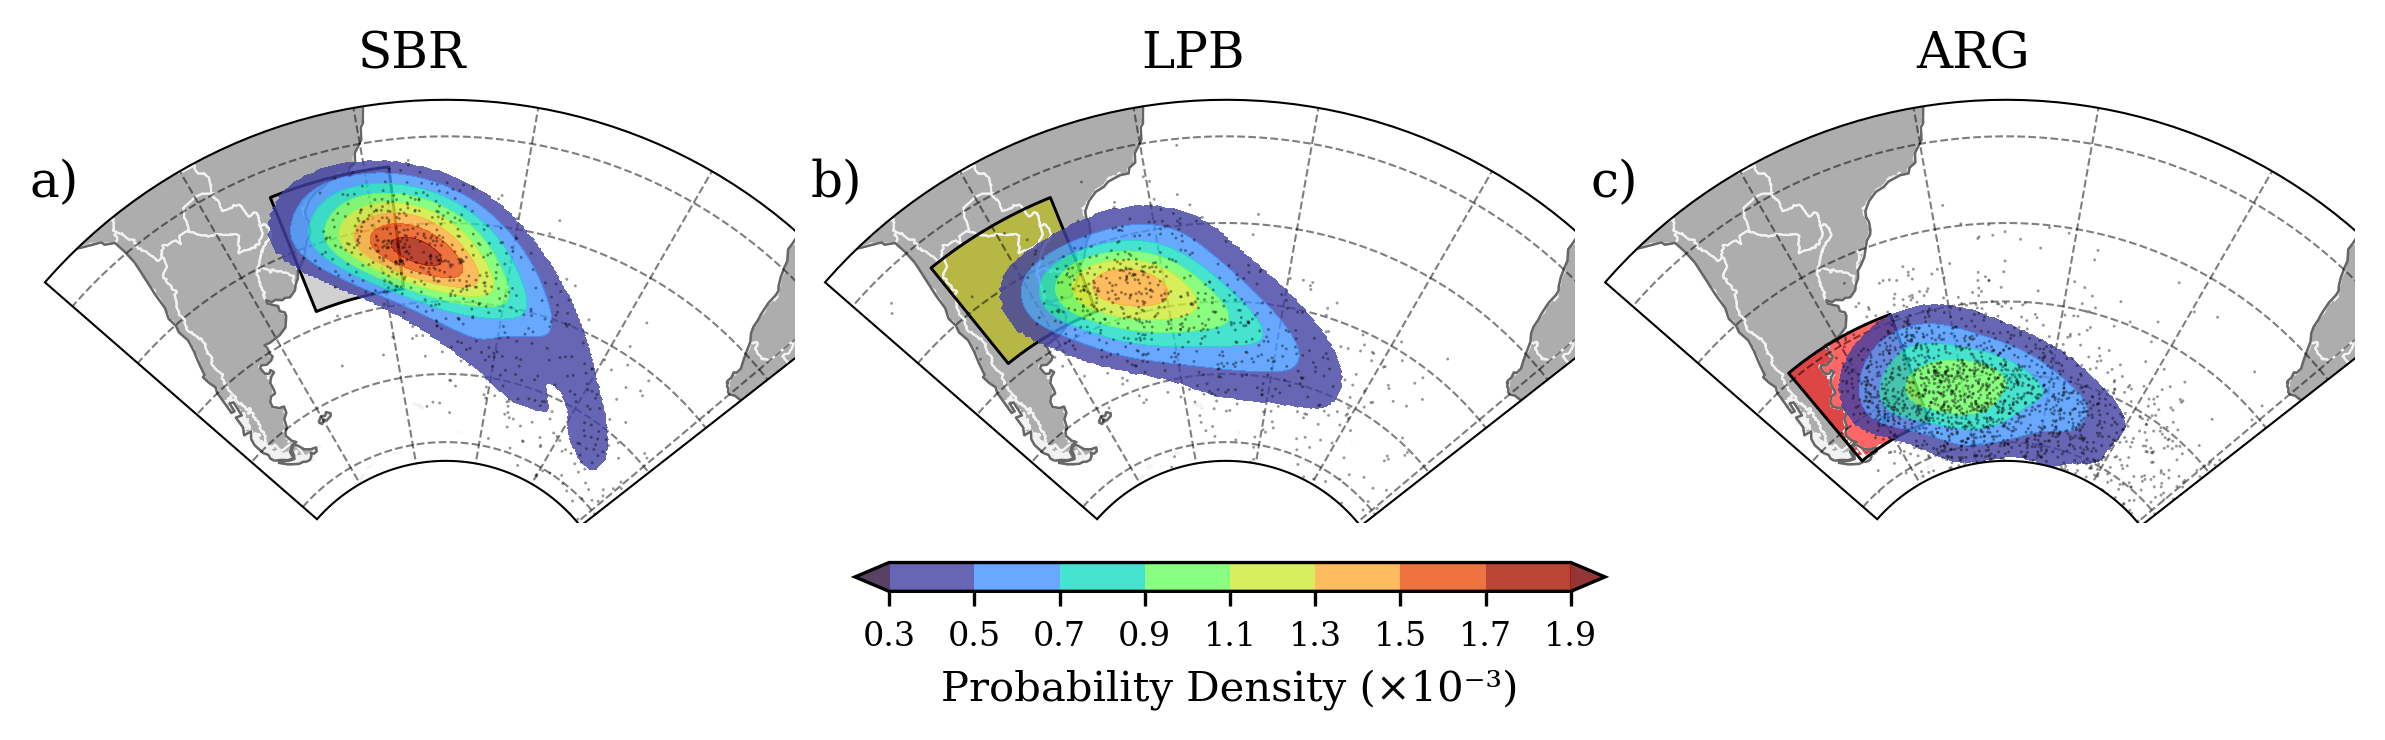
\includegraphics[width=\textwidth]{images/geral/vort_global_vf.png}
\caption[Localização do mínimo de vorticidade (População Global)]{Distribuição espacial da densidade de probabilidade da localização onde os ciclones da PG alcançam sua menor vorticidade relativa a 850~hPa ($\zeta_{850}^{\min}$) ao longo de seu ciclo de vida. a), b) e c) correspondem às regiões de ciclogênese SBR, LPB e ARG, respectivamente. Os contornos de cores indicam a densidade de probabilidade ($\times 10^{-3}$) e os pontos cinzas marcam as posições individuais dos mínimos.}
\label{fig:loc_vort_global}
\end{figure}


\subsection{Subconjunto de alta intensidade (p90)}\label{subsec:subconjuntos_intensidad}

Para avaliar os padrões espaciais em função da severidade dinâmica do sistema, extrai-se da PG, de forma independente para cada região de ciclogênese, os 10\% de ciclones com os valores mais negativos de $\zeta_{850}^{\min}$ (um decil da distribuição), obtendo o subconjunto $p90$ (detalhado em \ref{subsec:tb_poblaciones}).

A Tabela~\ref{tab:conteo_ciclones} documenta a redução do tamanho amostral desde a base bruta até a PG e o subconjunto p90.

\begin{table}[htbp]
\centering
\caption[Número de ciclones selecionados por região]{Número de ciclones selecionados por região. A coluna ``Total'' refere-se à base de trajetórias bruta e ``População Global'' aos sistemas com um ciclo de vida completo. A coluna ``Subconjunto'' indica o tamanho amostral para o subconjunto analisado (p90), equivalente a 10\% da População Global.}
\label{tab:conteo_ciclones}
\begin{tabular*}{\textwidth}{@{\extracolsep{\fill}}lccc}
\hline
Região & Total & População Global & Subconjunto \\
\hline
ARG & 4015 & 1980 & 198 \\
SBR & 1486 & 641  & 64  \\
LPB & 1288 & 669  & 67  \\
\hline
\end{tabular*}
\end{table}


A análise da fase em que se registra o pico de vorticidade (Tabela~\ref{tab:fase_max_intensidad}) mostra que p90 respeita a estrutura dinâmica dominante. Cerca de 83\% dos casos alcança sua intensidade máxima ($\zeta_{850}^{\min}$) durante a fase de maturidade, frente a menos de 5\% durante o decaimento.

\begin{table}[htbp]
\centering
\caption[Fase evolutiva de máxima intensidade dinâmica]{Distribuição percentual da fase evolutiva em que se registra a máxima intensidade dinâmica ($\zeta_{850}^{min}$), calculada como média entre as três regiões de ciclogênese.}
\label{tab:fase_max_intensidad}
\begin{tabular*}{\textwidth}{@{\extracolsep{\fill}}lcccc}
\hline
\textbf{Fase} & \textbf{População Global (\%)} & \textbf{p90 (\%)} \\
\hline
Incipiente       & $\sim$0.1 & ---  \\
Intensificação  & 13.2      & 11.7 \\
Maturidade       & 71.8      & 83.4 \\
Decaimento      & 14.9      & 4.9  \\
\hline
\end{tabular*}
\end{table}


A Figura~\ref{fig:loc_vort_p90} mostra a distribuição espacial da densidade de probabilidade da localização do mínimo de vorticidade do subconjunto p90.

% Figura para o subconjunto p90 (Subseção 2)
\begin{figure}[htbp]
\centering
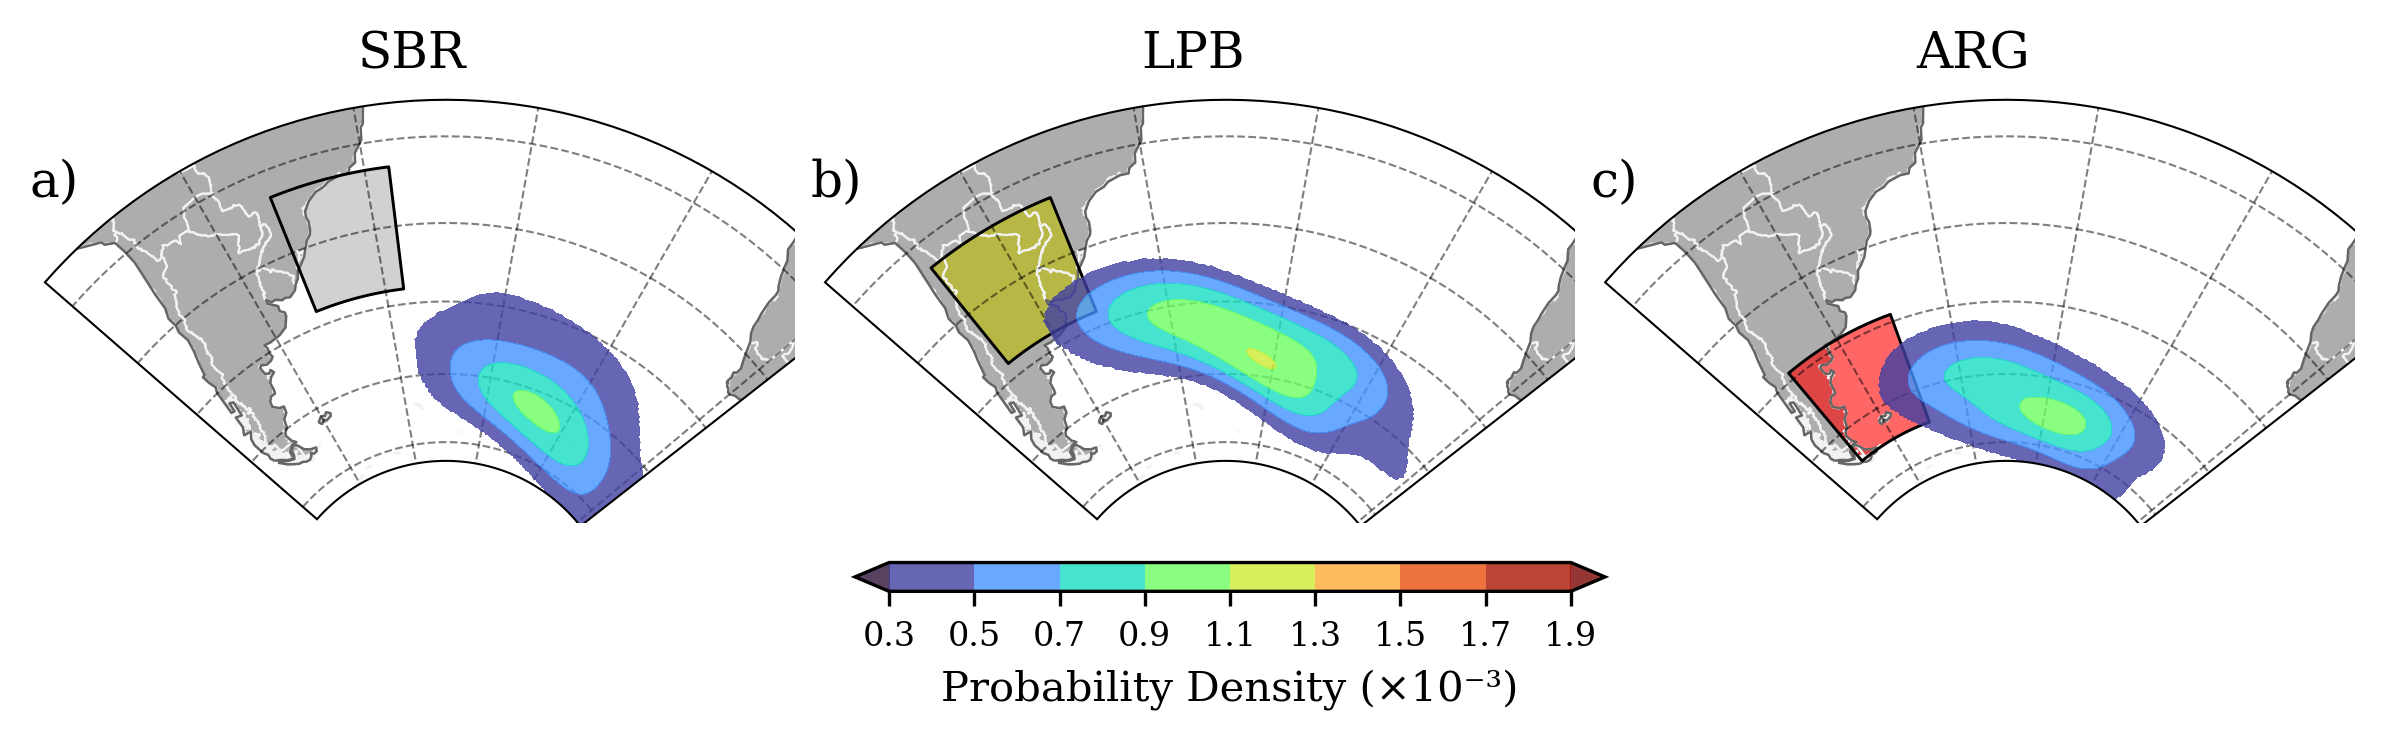
\includegraphics[width=\textwidth]{images/geral/vort_p90_vf.png}
\caption[Localização do mínimo de vorticidade (subconjunto p90)]{Semelhante à Figura~\ref{fig:loc_vort_global}, mas para o subconjunto p90 (sistemas mais intensos, decil inferior de $\zeta_{850}^{\min}$).}
\label{fig:loc_vort_p90}
\end{figure}

Sobre o subconjunto p90, comparando-o sistematicamente com a PG, aplica-se integralmente o fluxo metodológico descrito nas seções seguintes para avaliar se uma maior intensidade dinâmica do vórtice se associa a mudanças em: (i) a magnitude absoluta dos máximos de vento e precipitação; (ii) a distribuição espacial relativa desses máximos; e (iii) os padrões estruturais dominantes identificados pelo MEOF.

% ============================================================
%  SEÇÃO M3 — PROCESSAMENTO SEMILAGRANGEANO
% ============================================================

\section{Processamento semilagrangeano}\label{sec:procesamiento_lagrangiano}

Para caracterizar a estrutura dos sistemas independentemente de sua localização geográfica, adota-se o referencial semilagrangeano exposto na Seção~\ref{subsec:tb_lagrangiano} dos Fundamentos, um domínio móvel de $20^{\circ} \times 20^{\circ}$ centrado na posição do mínimo de vorticidade para cada instante $t$ da trajetória, em coordenadas relativas $(\Delta x, \Delta y)$ em relação ao núcleo ciclônico. Esse domínio isola o sinal de mesoescala e representa fisicamente a extensão espacial dos braços frontais do sistema, dimensão também usada por \citet{cardoso2022synoptic} no Atlântico Sul. O processamento é realizado separadamente para cada combinação de região de ciclogênese e fase do ciclo de vida.

Seguindo a técnica de compositing centrado no sistema (Seção~\ref{subsec:tb_compositing}), aplica-se uma média temporal centrada para reduzir a variabilidade de alta frequência dos dados horários e obter o campo mais representativo de cada fase. Para cada ciclone e fase, são promediados unicamente os registros horários mais próximos ao ponto médio temporal dessa fase: dois registros quando sua duração total é par (os dois passos centrais, equidistantes do ponto médio), e três quando é ímpar (o passo central exato mais um adjacente de cada lado). Esse critério evita que a média misture dois regimes evolutivos distintos, de modo que o campo resultante representa a condição arquetípica da fase (incipiente, intensificação, maturidade ou decaimento) e não uma transição entre estados sucessivos. O resultado é um único campo médio por combinação ciclone--fase, unidade de análise de todas as etapas estatísticas subsequentes. Consequentemente, cada ciclone contribui com exatamente um campo para cada uma das quatro populações fase-específicas de sua região, de modo que o tamanho amostral $m$ é constante entre fases dentro de uma mesma região e igual ao número de ciclones reportado na Tabela~\ref{tab:conteo_ciclones}.

% ============================================================
%  SEÇÃO M4 — CARACTERIZAÇÃO ESTATÍSTICA UNIVARIADA
% ============================================================

\section{Caracterização estatística univariada}\label{sec:tecnicas_estadisticas}

\subsection{Extração de máximos e distribuição de probabilidade (PDF)}\label{subsec:extraccion_pdf}

Sobre o campo médio por ciclone--fase aplica-se um suavizado espacial bidimensional com filtro gaussiano ($\sigma = 0.25$, biblioteca \texttt{scipy}) para evitar valores isolados em escala de ponto de grade. Em seguida, delimita-se a área de análise com uma máscara circular de $9.5^{\circ}$ de raio centrada no núcleo do sistema, inscrita no domínio de $20^{\circ} \times 20^{\circ}$ centrado no ciclone, de modo que uma faixa perimetral de $0.5^{\circ}$ em cada borda fica excluída. Dentro desse raio identificam-se: (i) a magnitude do valor máximo absoluto da variável de interesse, $x_i$, e (ii) sua localização em coordenadas relativas ao centro do ciclone, $\mathbf{s}_i = (\Delta x_i, \Delta y_i)$. O procedimento gera, para cada combinação de região, fase evolutiva e variável, um conjunto de $m$ pares magnitude--localização (um por evento ciclônico).

Para caracterizar a distribuição das magnitudes máximas extraídas $\{x_i\}_{i=1}^{m}$ estima-se a função de densidade de probabilidade (PDF) mediante KDE; sua justificativa em relação a histogramas e sua formulação matemática são apresentadas na Seção~\ref{subsec:tb_kde} dos Fundamentos. A implementação usa a classe \texttt{gaussian\_kde} de \texttt{scipy.stats}, com largura de banda $h$ segundo a regra de Scott (Equação~\ref{eq:scott_rule}) e o núcleo gaussiano (Equação~\ref{eq:tb_gaussian_kernel}) dos Fundamentos. As curvas PDF permitem contrastar quantitativamente como as magnitudes evoluem ao longo do ciclo de vida e como diferem entre a PG e p90.

\subsection{Distribuição espacial dos máximos}\label{subsec:kde_localizacion}

Para caracterizar a localização preferencial dos máximos em relação ao centro do ciclone, a posição relativa de cada máximo é tratada como variável aleatória bidimensional $\mathbf{S} = (\Delta x, \Delta y)$. A partir do conjunto de $m$ localizações relativas $\{\mathbf{s}_i\}_{i=1}^{m}$ da etapa anterior, estima-se a função de densidade de probabilidade da posição (PDFe), $\hat{f}(\mathbf{s})$, mediante o estimador kernel bidimensional da Seção~\ref{subsec:tb_kde} (Equações~\ref{eq:tb_kde_simple}--\ref{eq:tb_gauss_kernel_2d_simple}).

Diferentemente da PDF de magnitudes (Seção~\ref{subsec:extraccion_pdf}), a PDFe quantifica a densidade de probabilidade de que o máximo ocorra em uma posição relativa dada $\mathbf{s} = (\Delta x, \Delta y)$, independentemente do valor numérico de precipitação ou vento nesse ponto. O resultado é um campo contínuo de densidade de probabilidade sobre o domínio centrado.

\subsection{Análise de Funções Ortogonais Empíricas (EOF) univariada}\label{subsec:eof_univariado}

Para identificar os padrões espaciais dominantes de variabilidade estrutural, aplica-se uma análise EOF sobre o conjunto de $m$ campos médios por ciclone--fase, separadamente para cada variável (precipitação, vento), região e fase. As referências prévias desse enfoque foram apresentadas na Seção~\ref{subsec:tb_eof}. Antes da análise, subtrai-se de cada campo a média do conjunto em cada ponto de grade para obter as anomalias estruturais:

\begin{equation}\label{eq:eof_anomalia}
    X'(\tau, \mathbf{s}) = X(\tau, \mathbf{s}) - \frac{1}{m}\sum_{\tau'=1}^{m}X(\tau', \mathbf{s}),
\end{equation}

em que $X(\tau, \mathbf{s})$ é o campo da variável para o ciclone $\tau$ na posição relativa $\mathbf{s} = (x,y)$.

A análise EOF univariada se aplica em duas instâncias, com um tratamento ligeiramente distinto dessa anomalia segundo o propósito.

\paragraph{Modos dominantes e variância explicada.} Para as figuras de EOF1 e de fracionamento de variância (Seções~\ref{subsec:eof1_wind10_global}--\ref{subsec:eof1_wind10_p90}, \ref{subsec:eof1_tp_global}--\ref{subsec:eof1_tp_p90}, \ref{sec:var_exp_wind10} e \ref{subsec:var_exp_tp}), a anomalia é normalizada por um escalar global, com a mesma lógica aplicada ao MEOF (Seção~\ref{subsec:eof_multivariado}, Equação~\ref{eq:meof_normalizacion}):

\begin{equation}\label{eq:eof_normalizacion}
    Z(\tau, \mathbf{s}) = \frac{X'(\tau, \mathbf{s})}{\bar{\sigma}_X}, \qquad \bar{\sigma}_X = \frac{1}{N_s}\sum_{i=1}^{N_s} \sigma_X(\mathbf{s}_i),
\end{equation}

em que $\sigma_X(\mathbf{s}_i)$ é o desvio padrão entre ciclones no ponto de grade $\mathbf{s}_i$. Esse escalar único preserva a forma espacial da anomalia enquanto normaliza sua magnitude, e é calculado de forma independente para cada variável, região e fase mediante \texttt{scikit-learn}. Como consequência, as cargas de EOF$_k$ mostradas nos mapas são adimensionais (em unidades de $\bar\sigma_X$), não a magnitude física original da variável.

\paragraph{Significância estatística.} Para o teste Bootstrap-t (Seção~\ref{subsec:bootstrap_significancia}), o EOF é calculado diretamente sobre a anomalia $X'(\tau,\mathbf{s})$ sem essa etapa de normalização, mediante a biblioteca \texttt{xeofs} \citep{rieger2024xeofs} sobre estruturas \texttt{xarray}. Dado que ambos os procedimentos diferem unicamente por um fator de escala constante, igual para todo o domínio e todos os ciclones de um grupo, o percentual de variância explicada por cada modo é idêntico entre ambos; apenas muda a unidade das cargas espaciais, que nesse caso conservam a magnitude física original da variável.

Em ambos os casos, a reconstrução do campo a partir dos modos ortogonais segue a mesma expressão geral:

\begin{equation}\label{eq:eof_reconstruccion}
    X'(\tau, \mathbf{s}) = \sum_{k=1}^{K} \text{PC}_k(\tau) \cdot \text{EOF}_k(\mathbf{s}).
\end{equation}

Não se aplica remoção de tendência temporal (\textit{detrend}). O eixo amostral é um índice de eventos discretos com espaçamento temporal irregular entre 1979--2020, de modo que um ajuste linear cronológico assumiria erroneamente um espaçamento constante. O objetivo físico é isolar as características morfológicas da variabilidade inter-sistêmica dentro de cada fase, não as tendências climáticas de baixa frequência.

Cabe destacar que o tamanho amostral $m$ difere substancialmente entre regiões (Tabela~\ref{tab:conteo_ciclones}). ARG possui a amostra mais numerosa (1980 na PG, 198 em p90), enquanto SBR e LPB apresentam amostras consideravelmente menores (641/64 e 669/67, respectivamente). Essa assimetria implica que os autovetores de SBR e LPB estão sujeitos a maior incerteza de amostragem do que os de ARG, o que motiva a avaliação de significância estatística mediante Bootstrap-t descrita na Seção~\ref{subsec:bootstrap_significancia}.

A interpretação física de cada modo --como fluxo sinótico de fundo ou como circulação de mesoescala-- se apoia na escala espacial do padrão, sua localização relativa ao centro do ciclone e sua comparação qualitativa com a literatura; não se contrasta aqui com vento vetorial, diagnósticos frontais independentes ou índices de circulação de grande escala. Essas atribuições são lidas, portanto, como leituras fisicamente plausíveis, e não como identificações confirmadas.

\subsection{Significância espacial: Bootstrap-t}\label{subsec:bootstrap_significancia}

Para avaliar a robustez estatística dos autovetores do EOF e isolar os sinais físicos do ruído estocástico, implementa-se a reamostragem não paramétrica Bootstrap-t; sua escolha e vantagens em relação ao Bootstrap percentílico padrão para distribuições assimétricas e de cauda pesada foram fundamentadas na Seção~\ref{subsec:tb_bootstrap} dos Fundamentos. Geram-se $R = 15{,}000$ subamostras com reposição, garantindo erro de Monte Carlo insignificante na estimação das caudas da distribuição.

Para cada iteração $b$, recalcula-se o EOF sobre a subamostra e, em cada ponto de grade, calcula-se a estatística:

\begin{equation}\label{eq:bootstrap_t_espacial}
    t^*_b(\mathbf{s}) = \frac{\hat{\theta}^*_b(\mathbf{s}) - \hat{\theta}(\mathbf{s})}{SE^*_b(\mathbf{s})},
\end{equation}

em que $\hat{\theta}(\mathbf{s})$ é a carga espacial original em $\mathbf{s}$, $\hat{\theta}^*_b(\mathbf{s})$ sua estimativa na subamostra, $SE^*_b(\mathbf{s})$ o erro padrão dessa subamostra, e $SE(\mathbf{s})$ o erro padrão da carga original (calculado sobre a amostra completa, sem reamostrar). Os intervalos de confiança a 95\% são obtidos invertendo os quantis empíricos $q_{\alpha/2}$ e $q_{1-\alpha/2}$ da distribuição de $t^*$ (com $\alpha = 0.05$):

\begin{equation}\label{eq:bootstrap_ci_espacial}
    \left(\hat{\theta}(\mathbf{s}) - q_{1-\alpha/2}\,SE(\mathbf{s}),\; \hat{\theta}(\mathbf{s}) - q_{\alpha/2}\,SE(\mathbf{s})\right).
\end{equation}

Um ponto de grade é considerado estatisticamente significativo quando seu intervalo de confiança exclui o zero, o que equivale a rejeitar, no nível $\alpha = 0.05$ já definido, a hipótese nula de que a carga espacial nesse ponto não difere de zero por acaso de amostragem.

\subsection{Análise das Componentes Principais (PC1--PC3)}\label{subsec:analisis_pc}

Além da decomposição espacial, será usada a Componente Principal do primeiro modo (PC1), que representa a amplitude de cada ciclone sobre o padrão estrutural dominante; a interpretação dessas estatísticas foi estabelecida na Seção~\ref{subsec:tb_eof} dos Fundamentos.
Calculam-se, para a série de PC1 de cada variável, região e fase, a assimetria ($\gamma_1$):
\begin{equation}\label{eq:pc1_asimetria}
    \gamma_1 = \frac{1}{m} \sum_{\tau=1}^{m} \left(\frac{PC_{1,\tau} - \overline{PC_1}}{\sigma_{PC_1}}\right)^3,
\end{equation}
e a curtose ($\gamma_2$):
\begin{equation}\label{eq:pc1_curtosis}
    \gamma_2 = \frac{1}{m} \sum_{\tau=1}^{m} \left(\frac{PC_{1,\tau} - \overline{PC_1}}{\sigma_{PC_1}}\right)^4 - 3.
\end{equation}

Para conectar fisicamente a estrutura dos campos de superfície com a intensidade do sistema, avalia-se a correlação de Spearman entre a PC1, a PC2 e a PC3 de cada variável, e a vorticidade relativa a 850 hPa associada.
Esta última é obtida dos mesmos instantes centrais usados para construir os campos compostos (Seção~\ref{sec:procesamiento_lagrangiano}), tomando o de maior magnitude entre eles como representativo da intensidade do sistema nessa fase; não deve ser confundida com o $\zeta_{850}^{\min}$ de toda a vida do ciclone empregado na Seção~\ref{subsec:grupo_global} para a seleção do subconjunto p90.

O sinal da PC indica de forma reprodutível a que lado do padrão dominante cada ciclone recai.
Correlacionar a PC com sinal contra uma variável externa testa, então, se esse lado do padrão está associado à intensidade do sistema, além do quão marcada esteja a projeção.
Emprega-se Spearman para não assumir normalidade na distribuição das PC.
Sua interpretação físico-estatística, o vínculo entre o lado do padrão dominante em que recai um ciclone e sua intensidade dinâmica, foi estabelecida na Seção~\ref{subsec:tb_eof} dos Fundamentos.
Dado que o sinal de cada EOF é uma convenção independente e arbitrária entre decomposições distintas (Seção~\ref{subsec:tb_eof}), comparar o sinal dessa correlação entre regiões, fases ou populações não é informativo por si só; os capítulos de resultados reportam, por isso, o valor absoluto da correlação, e discutem sua magnitude e significância estatística em vez de seu sinal.

Para avaliar se os padrões dominantes de precipitação e vento variam conjuntamente, calcula-se a correlação de Spearman entre a PC1 de precipitação e a PC1 do vento, dentro de cada região e fase.
Valores próximos a $+1$ ou a $-1$ indicam que o lado do padrão dominante de um campo está sistematicamente associado ao lado do padrão dominante do outro; valores próximos a $0$ sugerem que ambos os padrões variam de forma independente entre si.
Pela mesma razão, o sinal dessa correlação cruzada só é interpretável se se verifica explicitamente, para a região e fase específicas, onde se localiza o núcleo de carga positiva de cada EOF1; fora desse contexto verificado, reporta-se o valor absoluto.

% ============================================================
%  SEÇÃO M5 — ANÁLISE MULTIVARIADA E PROTÓTIPOS
% ============================================================

\section{Análise multivariada e protótipos estruturais}\label{sec:meof_prototipos}

\subsection{EOF combinado (MEOF) precipitação--vento}\label{subsec:eof_multivariado}

Para identificar os padrões espaciais dominantes da estrutura combinada de precipitação e vento, realiza-se uma análise EOF combinada (MEOF). Diferentemente da análise univariada, o MEOF captura modos de variabilidade conjunta que refletem a organização morfológica típica dos campos de superfície associados à dinâmica ciclônica. Os fundamentos dessa técnica, incluindo a necessidade de normalizar variáveis com unidades físicas dispares e a lógica da concatenação espacial do vetor de estado, foram expostos na Seção~\ref{subsec:tb_eof} dos Fundamentos. Embora o MEOF seja habitual em estudos de eventos simultâneos, aqui se emprega exclusivamente como ferramenta de síntese estrutural, para isolar as configurações espaciais mais recorrentes dos campos de superfície. O procedimento consta de três passos:

\paragraph{Passo 1 — Anomalias.} Calcula-se o campo de anomalias de cada variável em relação à média do conjunto (PG ou p90) em cada ponto de grade.

\paragraph{Passo 2 — Normalização por desvio padrão espacialmente promediado.} Para preservar os gradientes espaciais nativos de cada campo, a normalização usa um escalar global por variável, em vez da padronização ponto a ponto da PCA sobre matriz de correlação:
\begin{equation}\label{eq:meof_normalizacion}
    Z_{V}(\tau, \mathbf{s}) =
        \frac{V'(\tau, \mathbf{s})}{\bar{\sigma}_{V}},
    \qquad
    \bar{\sigma}_{V} = \frac{1}{N_s} \sum_{i=1}^{N_s} \sigma_{V}(\mathbf{s}_i),
\end{equation}
em que $V'$ é o campo de anomalias, $\sigma_{V}(\mathbf{s}_i)$ o desvio padrão entre eventos no ponto de grade $\mathbf{s}_i$, e $N_s$ o número de pontos de grade do domínio. Esse escalar preserva os gradientes espaciais enquanto equilibra o peso de ambas as variáveis na matriz de covariância, evitando que o campo de maior variância domine a decomposição conjunta, problema documentado para variáveis de unidades dispares em \citet{wilks2019statistical_ch13}.

\paragraph{Passo 3 — Concatenação espacial.} Os campos normalizados são concatenados para formar o vetor de estado combinado:

\begin{equation}\label{eq:meof_vector}
    \mathbf{Y}(\tau) = \big[ Z_P(\tau),\; Z_W(\tau) \big].
\end{equation}

O EOF aplicado à matriz combinada $\mathbf{Y}(\tau)$ produz modos conjuntos que explicam a variância conjunta do sistema. O MEOF$_1$ produz simultaneamente um padrão espacial para precipitação ($\text{EOF}_{1,P}$) e outro para vento ($\text{EOF}_{1,W}$), ambos extraídos do mesmo modo dominante de covariabilidade conjunta.

Tanto a PG quanto o subconjunto p90 são processados de forma independente com esse mesmo procedimento, de modo que os padrões estruturais resultam exclusivamente de sua própria covariância interna.

\subsection{Construção dos protótipos estruturais}\label{subsec:prototipos}

Para cumprir o Objetivo Específico 4, desenvolve-se um procedimento de síntese visual que integra em um único painel, para cada combinação região-fase, quatro fontes de informação estatística derivadas das análises anteriores. Cada protótipo se compõe de quatro camadas superpostas em coordenadas relativas ao centro do ciclone $(\Delta x, \Delta y)$, dentro do domínio de $9.5^{\circ}$ de raio. A lógica do compositing centrado no sistema, que torna possível essa superposição, foi apresentada na Seção~\ref{subsec:tb_compositing} dos Fundamentos.

As duas primeiras camadas são as isolinhas da PDFe da localização de máximos de precipitação e vento. A partir da superfície de densidade $\hat{f}(\mathbf{s})$ (Equação~\ref{eq:tb_kde_simple}) extraem-se os contornos dos percentis 75 e 90 da densidade acumulada, e sobre cada superfície sinaliza-se com um marcador a coordenada $(\Delta x_{\text{moda}}, \Delta y_{\text{moda}})$, a posição onde é mais frequente encontrar o máximo da variável.

As camadas terceira e quarta mostram as isolinhas dos padrões espaciais do primeiro modo EOF univariado de cada campo ($\text{EOF}_{1,P}$ para precipitação e $\text{EOF}_{1,W}$ para vento), obtidos segundo a Seção~\ref{subsec:eof_univariado} e não do modo conjunto MEOF$_1$ (Seção~\ref{subsec:eof_multivariado}); essa escolha é justificada no Capítulo~\ref{cap:prototipos}.
Antes do traçado de contornos, aplica-se um suavizado gaussiano ($\sigma = 2$) a cada campo. Os níveis de contorno são determinados mediante percentis aplicados separadamente sobre os valores positivos (percentis 33 e 66, linha sólida) e negativos (percentis 33 e 66 do valor absoluto, linha descontínua).
Essa limiarização relativa garante comparabilidade entre diferentes combinações região--fase, independentemente da magnitude absoluta do padrão espacial do EOF.
As regiões de carga positiva indicam setores onde a variável tende a apresentar anomalias positivas em relação à média quando o modo dominante se ativa; as de carga negativa, supressão relativa.

O resultado se organiza em uma figura matricial de $3 \times 4$ painéis (3 regiões de ciclogênese $\times$ 4 fases evolutivas), em que cada painel integra as quatro camadas descritas: PDFe de precipitação, PDFe de vento, $\text{EOF}_{1,P}$ de precipitação e $\text{EOF}_{1,W}$ de vento.
A superposição permite ler o grau de organização espacial entre ambos os campos no entorno do ciclone: uma alta coincidência entre o núcleo do PDFe de precipitação e a região de carga positiva do EOF de vento indica uma estrutura frontal compacta; uma separação entre ambos revela assimetrias na distribuição dos máximos.
Essa análise caracteriza a morfologia da fase e, de forma secundária, oferece um referencial para identificar configurações que favoreceriam eventos simultâneos de vento e precipitação.

A coordenada de cada variável, anotada na legenda interna de cada painel como $(\Delta x, \Delta y)$ em graus, quantifica o deslocamento preferencial dos máximos em relação ao centro do vórtice.
Esse procedimento é executado de forma independente para a PG e o subconjunto p90, permitindo a comparação direta dos padrões estruturais entre ambos os estratos de intensidade.
		% trabalho.
\chapter{Vento a 10 metros}\label{cap:resultados_wind10}

Nos ciclones extratropicais (ETC), o vento em superfície favorece a formação de ondas anômalas \citep{gramcianinov2023impact}.
Esse vento responde a processos de diferentes escalas, como o fluxo sinótico, os jatos de mesoescala, as correntes descendentes e a seclusão quente (Seção~\ref{subsec:tb_modelos}).
Consequentemente, sua intensidade e distribuição espacial diferem entre ciclones, desde sistemas fracos dominados pelo fluxo de fundo até sistemas intensos que concentram os ventos mais fortes em setores específicos.

Este capítulo descreve a distribuição espacial do vento a 10 metros durante o ciclo de vida dos ETC formados nas três regiões de estudo (SBR, LPB e ARG), com três objetivos: (i)~quantificar a variação da magnitude do vento segundo a intensidade do ciclone e sua região de gênese, (ii)~identificar a localização preferencial dos máximos de vento em relação ao centro do ciclone, e (iii)~identificar os padrões dominantes de variabilidade espacial do vento e sua evolução entre fases.
A Seção~\ref{sec:pdf_wind10} compara as distribuições de magnitude (PDF) da População Global (PG) e do subconjunto de ciclones intensos (p90; Seção~\ref{subsec:subconjuntos_intensidad}).
As Seções~\ref{sec:kde_espacial_global} e~\ref{sec:kde_espacial_p90} analisam a localização dos máximos mediante sua densidade espacial (PDFe; Seção~\ref{subsec:kde_localizacion}), e as Seções~\ref{sec:var_exp_wind10}--\ref{subsec:res_dinamica_pc1} aplicam funções ortogonais empíricas (EOF; Seção~\ref{subsec:eof_univariado}) para identificar os padrões dominantes.
O Capítulo~\ref{cap:resultados_tp} aplica a mesma análise à precipitação, e o Capítulo~\ref{chap:meof} avalia se os máximos de ambas as variáveis coincidem no espaço (Seção~\ref{sec:tb_compound_def}).

% --- SEÇÃO PRINCIPAL: PDF DE VENTO A 10 METROS,
\section{Distribuição de magnitudes (PDF)}\label{sec:pdf_wind10}

A Figura~\ref{fig:pdf_wind10} apresenta as funções de densidade de probabilidade (PDF) dos máximos de vento a 10~m, extraídos do domínio centrado no ciclone (Seção~\ref{subsec:extraccion_pdf}), para as duas populações de estudo (Seção~\ref{sec:poblaciones_estudio}).
Os painéis se organizam por região de ciclogênese (SBR, LPB e ARG; Seção~\ref{sec:tb_regiones}) e por fase do ciclo de vida (Ic, It, M e D; Seção~\ref{subsec:tb_fases}).

Na fase incipiente (Ic; painéis a, b e~c), ambas as populações apresentam distribuições unimodais que se superpõem em grande parte, com picos entre 11 e 15~m\,s$^{-1}$.
Na intensificação (It; painéis d, e e~f) e na maturidade (M; painéis g, h e~i), a curva de p90 se desloca para valores maiores e alcança na maturidade um pico entre 23 e 25~m\,s$^{-1}$, com caudas de até 30~m\,s$^{-1}$.
Nessa fase, a População Global apresenta seu máximo entre 16 e 19~m\,s$^{-1}$ e uma distribuição mais larga.
Entre regiões, os picos de p90 na maturidade são mais altos em LPB (h) e ARG (i) (${\sim}0.19$) do que em SBR (g) (${\sim}0.17$), cuja distribuição é mais larga por um ombro em direção a 22--23~m\,s$^{-1}$, enquanto ARG estende sua cauda até os 30~m\,s$^{-1}$.
No decaimento (D; painéis j, k e~l), as curvas de p90 se deslocam para magnitudes menores e se alargam, embora se mantenham acima da População Global, com maior superposição em ARG.

\begin{figure}[htbp]
\centering
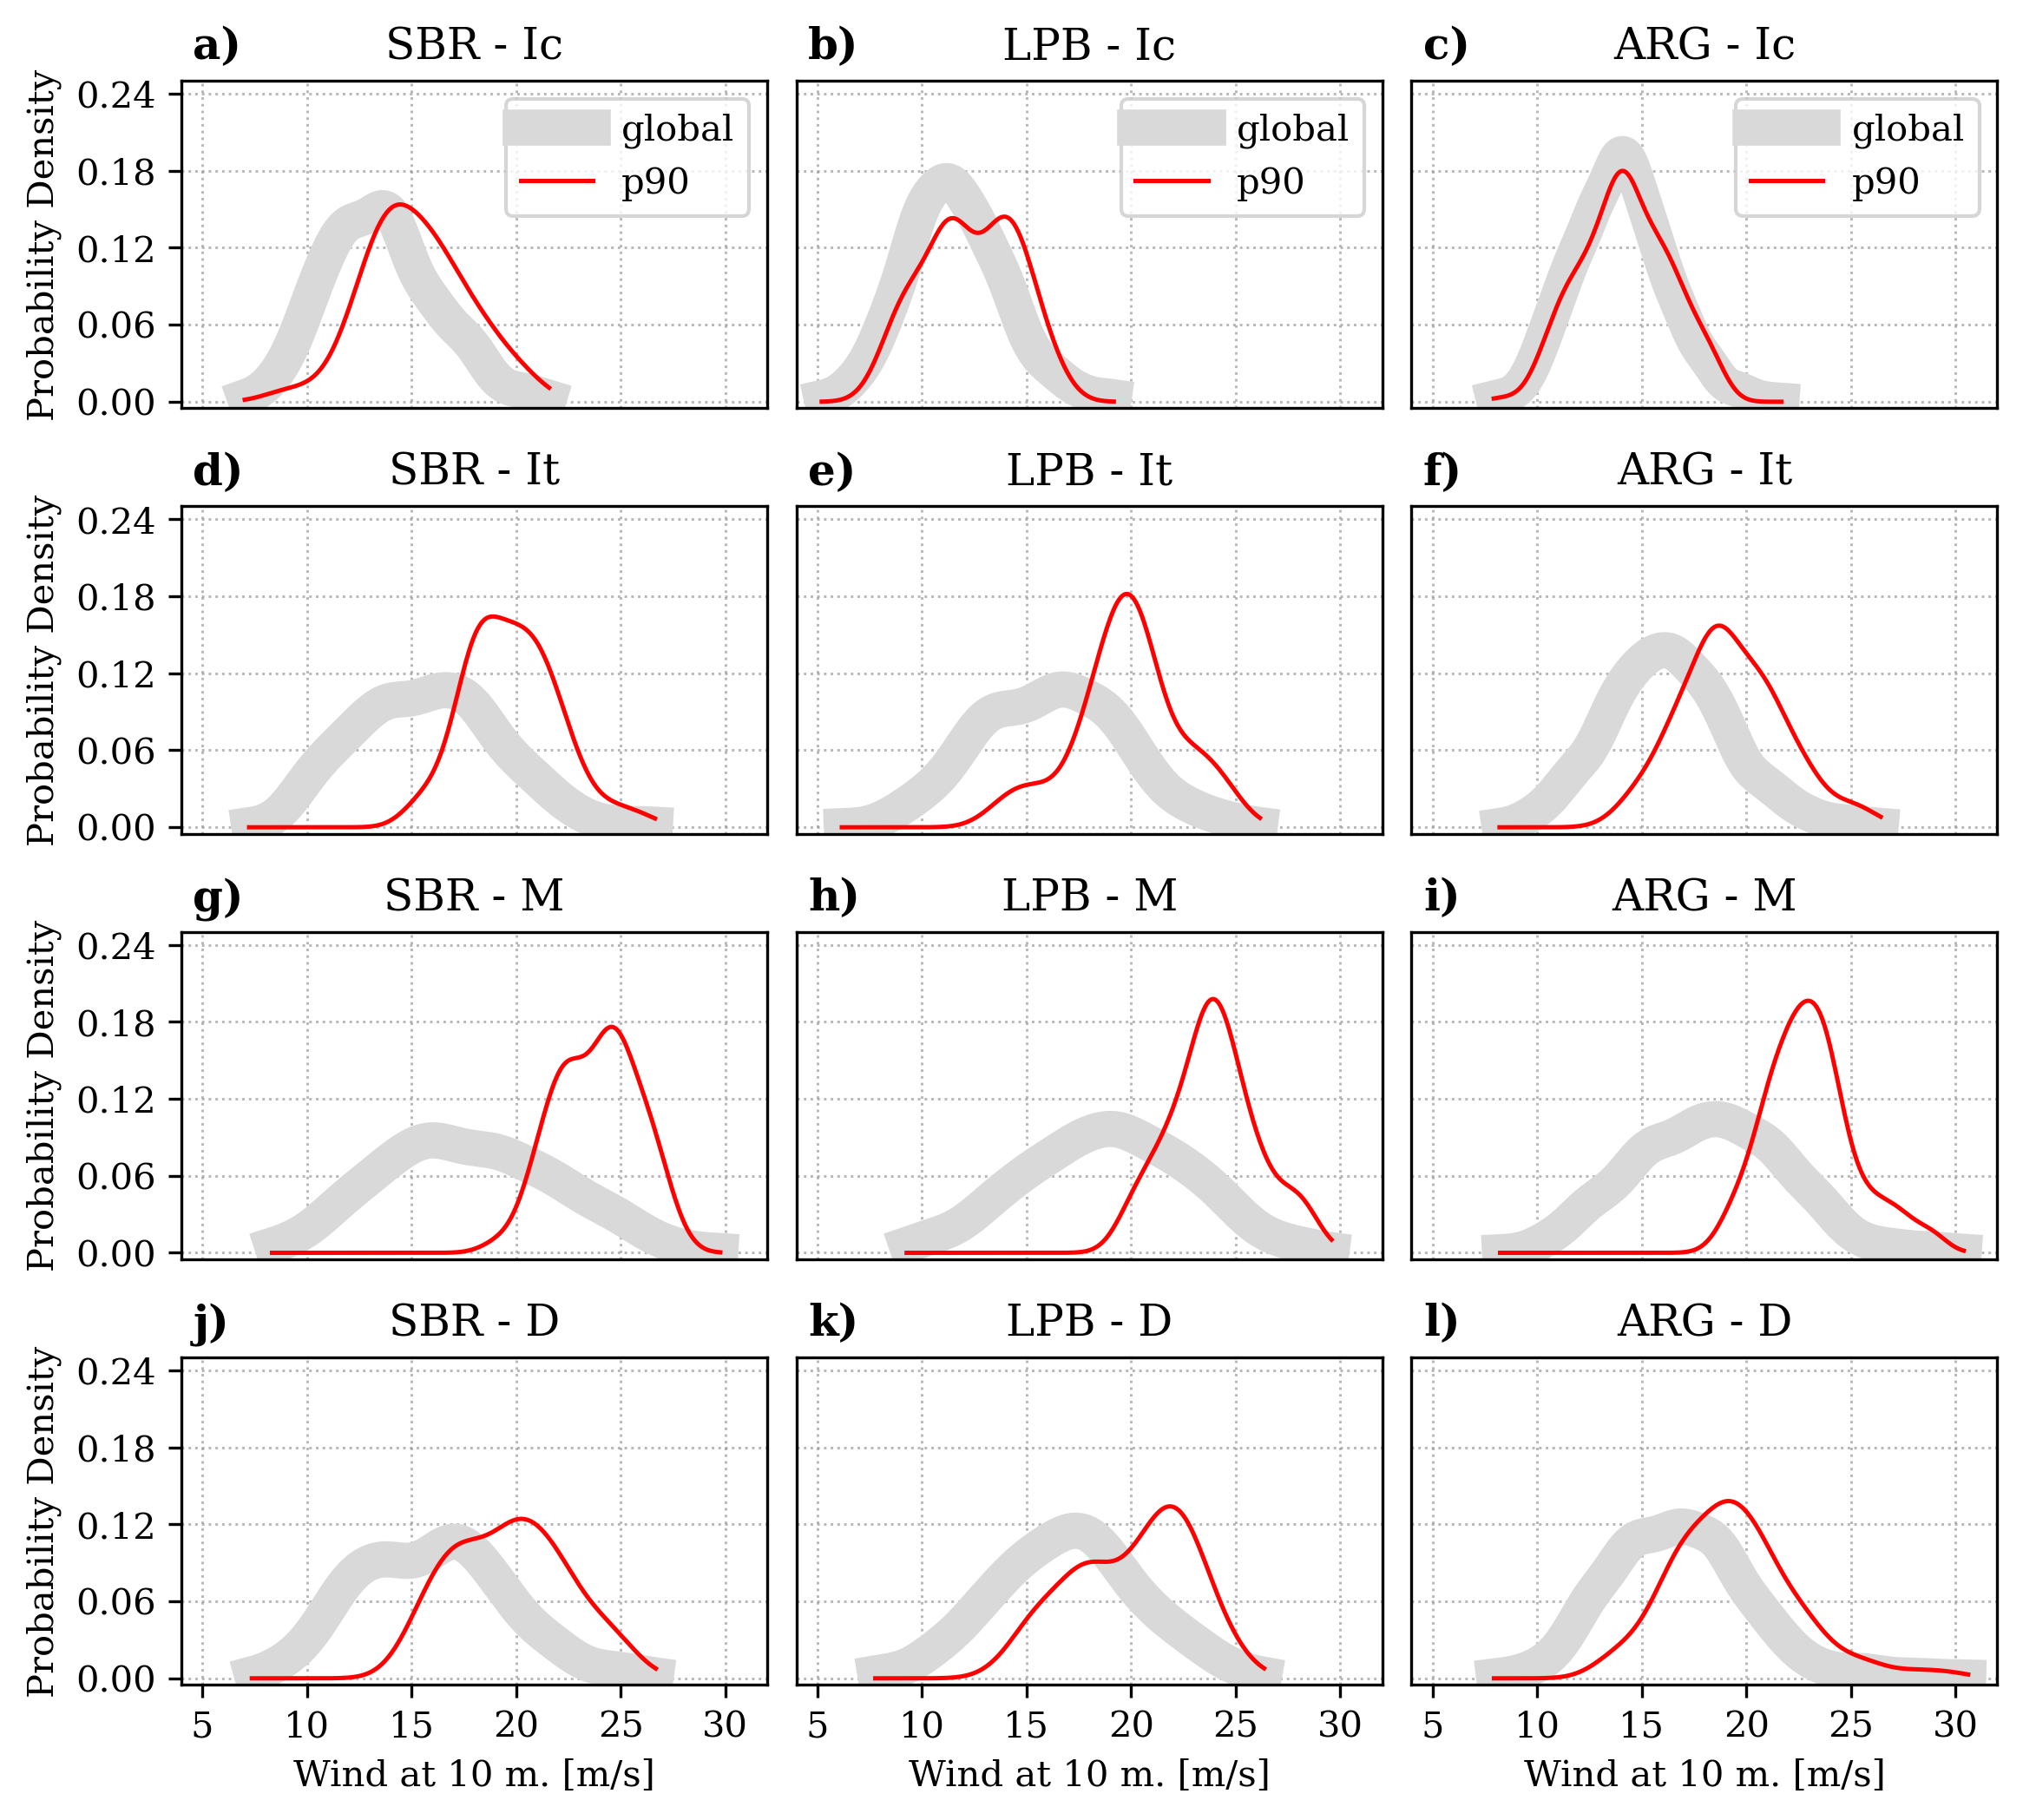
\includegraphics[width=\textwidth]{images/w10/PDF_wind10_sigma025.png}
\caption[PDF de magnitudes máximas de vento a 10 metros]{Funções de densidade de probabilidade (PDF) para as magnitudes máximas de vento a 10 metros. As colunas indicam a região de ciclogênese (SBR, LPB, ARG) e as linhas a evolução ao longo das fases do ciclo de vida (Ic, It, M, D). Contrasta-se a População Global (referência, sombreado cinza) com o subconjunto p90, formado pelos 10\% de ciclones de maior intensidade em vorticidade relativa a 850~hPa (Seção~\ref{subsec:subconjuntos_intensidad}), em linha vermelha.}
\label{fig:pdf_wind10}
\end{figure}

A maior separação entre distribuições ocorre na maturidade, fase em que a maioria dos ciclones alcança seu mínimo de vorticidade a 850~hPa, tanto na População Global quanto em p90 (Tabela~\ref{tab:fase_max_intensidad}).
\citet{gramcianinov2019properties}, a partir do vento máximo a 925~hPa, associam os ciclones de SBR e LPB a ventos intensos e apontam LPB como a região com os ciclones mais intensos do Atlântico Sul, e atribuem a ciclogênese ao norte de 35\textdegree S ao forçamento de níveis baixos ligado ao transporte de umidade no verão (Seções~\ref{subsec:tb_sbr} e~\ref{subsec:tb_lpb}). Nos dados aqui analisados, a moda da População Global na maturidade é maior em LPB (19~m\,s$^{-1}$) e ARG (18.5~m\,s$^{-1}$) do que em SBR (16~m\,s$^{-1}$), enquanto os picos de p90 são semelhantes entre regiões.

Em ARG, a baroclinicidade associada à frente e a perturbação topográfica dos Andes (Seção~\ref{subsec:tb_arg}) poderiam gerar respostas do vento mais variáveis, compatíveis com a cauda mais estendida em direção a velocidades altas que apresenta sua distribuição p90 na maturidade e no decaimento.
Apesar da menor disponibilidade de umidade, \citet{gramcianinov2024early} mostram que a amplificação da onda baroclínica em níveis baixos produz em ARG, durante a etapa inicial, ciclones com pressão central mais baixa do que em SBR e LPB, consistente com o regime mais baroclínico que caracteriza essa região.

A separação entre p90 e a População Global, que aumenta à medida que os ciclones maturam, mostra que a maior intensidade em vorticidade a 850~hPa, critério com o qual se define p90 (Seção~\ref{sec:poblaciones_estudio}), se traduz em ventos mais intensos em superfície.
Na maturidade, a moda de p90 se situa entre 23 e 25~m\,s$^{-1}$, entre 25\% (LPB e ARG) e 50\% (SBR) acima da moda da População Global (16--19~m\,s$^{-1}$), com caudas de até 30~m\,s$^{-1}$.
Esses valores são coerentes com os reportados para ciclones do Atlântico Sul \citep{padilhareinke2026characterization, gramcianinov2020analysis}.
\citet{padilhareinke2026characterization} documentam para o conjunto do Atlântico Sul-Ocidental um limiar p90 de 23.4~m\,s$^{-1}$ (84.4~km\,h$^{-1}$) e extremos de até 31.4~m\,s$^{-1}$ (113.2~km\,h$^{-1}$).
Esse limiar é semelhante ao máximo médio (${\sim}$25~m\,s$^{-1}$) do composto dos 100 ciclones mais intensos do Atlântico Norte no momento de máxima vorticidade \citep{gentile2025response}, embora se trate de outra população e outra bacia.
\citet{gramcianinov2020analysis} reportam para o inverno austral (JJA) no ERA5 velocidades máximas médias de 21.2\,$\pm$\,4.8~m\,s$^{-1}$ (percentil~90: 27.3~m\,s$^{-1}$; percentil~95: 29.3~m\,s$^{-1}$).\footnote{Na reanálise CFSR/CFSv2, os valores são ligeiramente superiores, 23.4\,$\pm$\,4.8~m\,s$^{-1}$ (percentil~90: 30.2~m\,s$^{-1}$; percentil~95: 32.1~m\,s$^{-1}$) \citep{gramcianinov2020analysis}.}
\citet{gramcianinov2023impact} destacam que as ondas extremas geradas pelos ventos desses ciclones têm um impacto considerável nas atividades costeiras e marítimas.

% --- SEÇÃO PRINCIPAL: KDE ESPACIAL DE VENTO A 10 METROS,

\section{Distribuição espacial de máximos (PDFe)}\label{sec:pdfe_wind10}
\subsection{População Global}\label{sec:kde_espacial_global}

\begin{figure}[htbp]
\centering
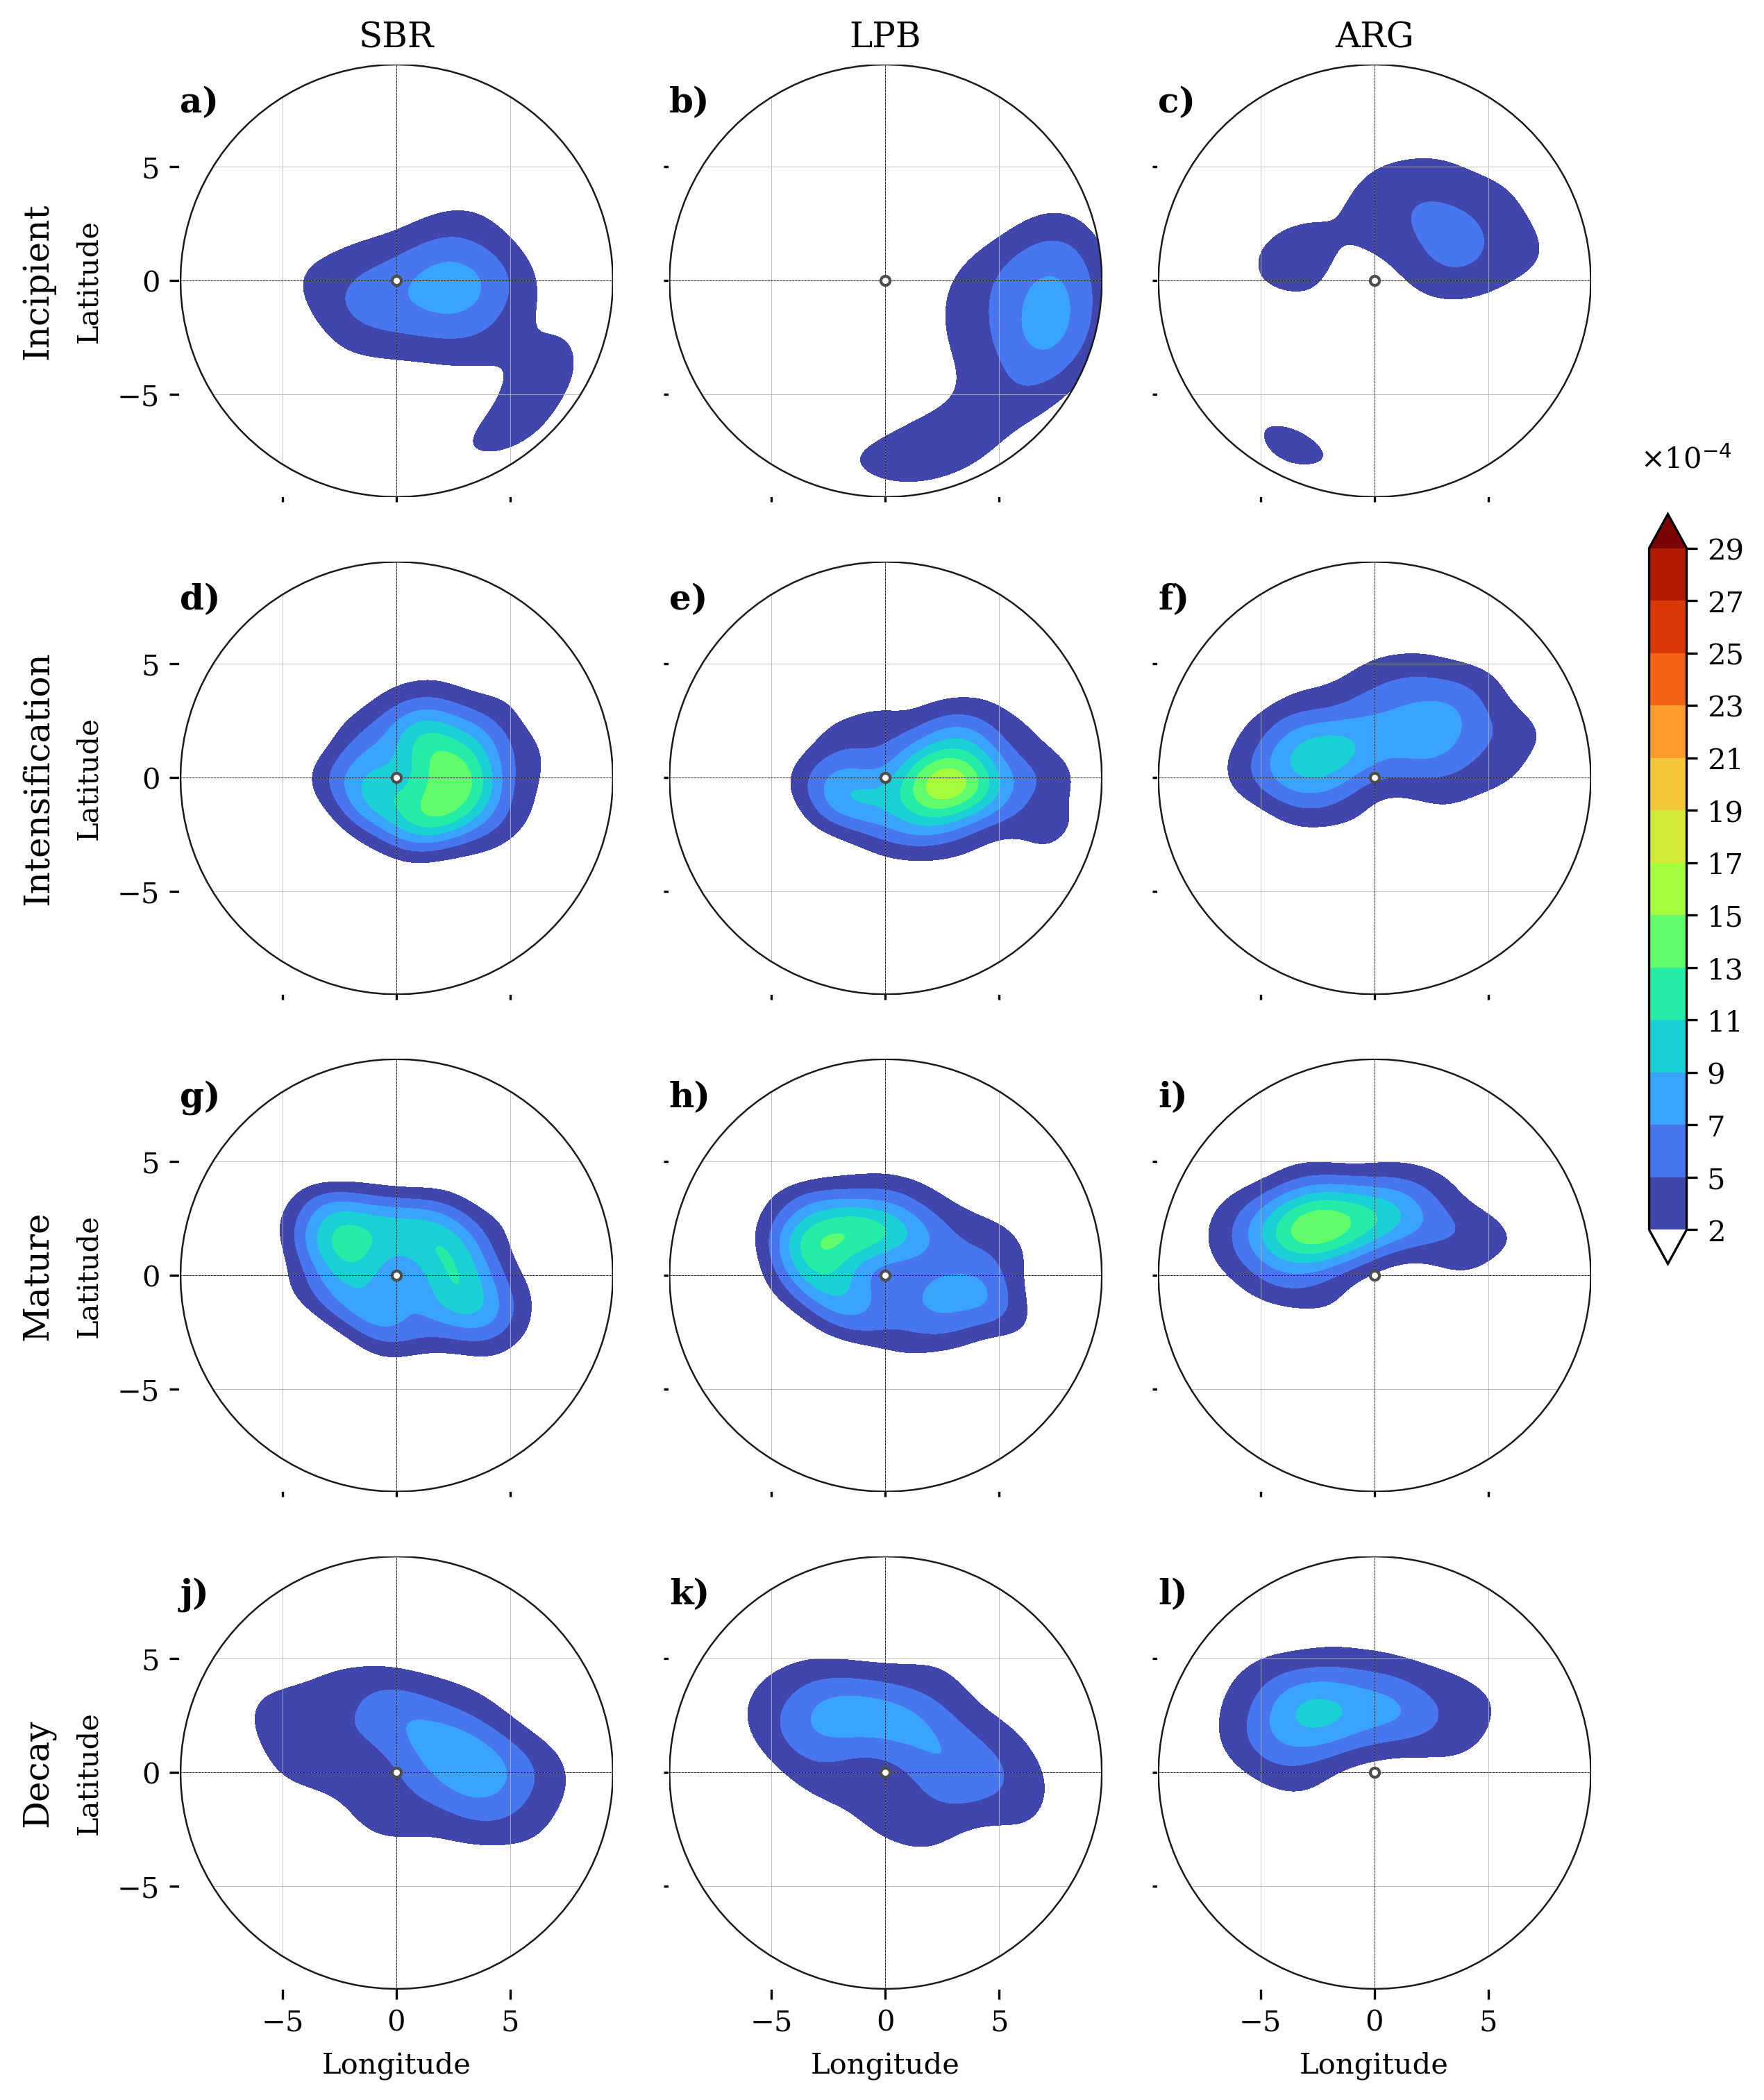
\includegraphics[width=\textwidth]{images/w10/kde_wind10_global_fasesxreg.png}
\caption[PDF espacial de vento máximo a 10 metros (População Global)]{Estimação de densidade espacial bidimensional (PDFe; Seção~\ref{subsec:kde_localizacion}) da localização dos máximos de magnitude de vento a 10~metros para a População Global. As colunas separam as regiões de ciclogênese (SBR, LPB, ARG) e as linhas indicam as fases evolutivas (Ic, It, M, D). O domínio está centrado no ciclone ($0^{\circ}, 0^{\circ}$).}
\label{fig:kde_wind_global}
\end{figure}

A Figura~\ref{fig:kde_wind_global} apresenta a densidade espacial da localização dos máximos de vento no domínio centrado no ciclone de $20^{\circ} \times 20^{\circ}$ (Seção~\ref{sec:procesamiento_lagrangiano}).
As distribuições são amplas e com gradientes suaves, e sua densidade máxima é menor do que a de p90 sobretudo na maturidade, nas três regiões ($11$--$15$ contra $19$--$27\times10^{-4}$). Nas demais fases as diferenças são menores e não seguem um sentido único. Em cinco dos nove casos a População Global chega a apresentar maior densidade, na fase incipiente de LPB e ARG, na intensificação de LPB e no decaimento de SBR e ARG.
Essa dispersão é a esperada em uma população heterogênea, já que a detecção por vorticidade também inclui centros móveis e menos profundos que a detecção por pressão omite \citep{sinclair1994objective}.

Na População Global, o núcleo de máxima densidade se localiza a leste do centro durante as fases incipiente e intensificação em SBR e LPB, e no quadrante noroeste durante a maturidade nas três regiões. Em ARG, esse deslocamento para o noroeste já ocorre durante a intensificação.
Na fase incipiente (Ic; painéis a, b e~c), as zonas de maior densidade abrangem áreas extensas e assimétricas, com o núcleo no setor leste (nordeste em ARG), o que concorda com sistemas que ainda não organizaram uma circulação fechada (Seção~\ref{subsec:tb_fases}).
Esse padrão é coerente com o observado por \citet{dejesus2021multimodel} nas reanálises, em que os ventos mais fortes em 1000~hPa ocupam o setor quente (nordeste no HS) do ciclone incipiente, embora sua amostra se restrinja às ciclogêneses mais intensas (quartil superior de vorticidade inicial) e seus compostos não estejam centrados no ciclone.
Durante a intensificação (It; painéis d, e e~f), as distribuições se tornam mais compactas e próximas do centro. Em SBR (d) e LPB (e) o núcleo permanece a leste, com a maior densidade dessa fase em LPB (${\approx}$\,15--17\,$\times10^{-4}$), enquanto em ARG (f) se localiza a oeste-noroeste e apresenta uma distribuição mais alongada em sentido zonal.
Na maturidade (M; painéis g, h e~i), o foco principal se situa no quadrante noroeste nas três regiões, com densidades de ${\approx}$\,11--15\,$\times10^{-4}$, e as diferenças regionais são discutidas a seguir.
No decaimento (D; painéis j, k e~l), as densidades diminuem até valores próximos aos da fase incipiente, e a localização do núcleo varia entre regiões, a leste-nordeste em SBR e a noroeste em LPB e ARG.

Na maturidade, ARG (i) apresenta um único núcleo no noroeste (${\approx}$\,13--15\,$\times10^{-4}$), enquanto SBR (g) e LPB (h) mostram um foco principal no noroeste e outro secundário a leste ou sudeste, com densidades máximas de ${\approx}$\,11--13\,$\times10^{-4}$ em SBR e ${\approx}$\,13--15\,$\times10^{-4}$ em LPB. Essa ordem regional não se repete na magnitude do vento (Seção~\ref{sec:pdf_wind10}), onde LPB e ARG apresentam os picos de densidade mais altos e SBR a distribuição mais larga, o que indica que a região que mais concentra a localização de seus máximos não é a que mais concentra sua intensidade.
Em ARG, esse padrão seria compatível com a advecção térmica e a perturbação topográfica andina, e em SBR e LPB com a advecção de ar quente e úmido (Seção~\ref{sec:tb_regiones}).

A dispersão da População Global reflete também a variabilidade na distância entre o centro e os ventos máximos. Em ciclones subtropicais do Atlântico Sul, \citet{gozzo2014subtropical} e \citet{cardoso2020wind} situam esses máximos entre 300 e 450~km e entre 400 e 500~km do centro, respectivamente, escalas que servem de referência ainda que não correspondam à população de ETCs aqui estudada. Essa heterogeneidade justifica separar os ciclones por intensidade (Seção~\ref{subsec:subconjuntos_intensidad}) e é coerente com o apontado por \citet{corner2025classification} para ciclones do Atlântico Norte e Europa, onde nem a pressão mínima nem a vorticidade máxima se relacionam bem com os impactos do ciclone, devido a estruturas de mesoescala que modulam o campo de vento. A seção seguinte analisa a localização dos máximos nos ciclones intensos, com essa população como referência.

\subsection{Subconjunto de ciclones intensos p90}\label{sec:kde_espacial_p90}

\begin{figure}[htbp]
\centering
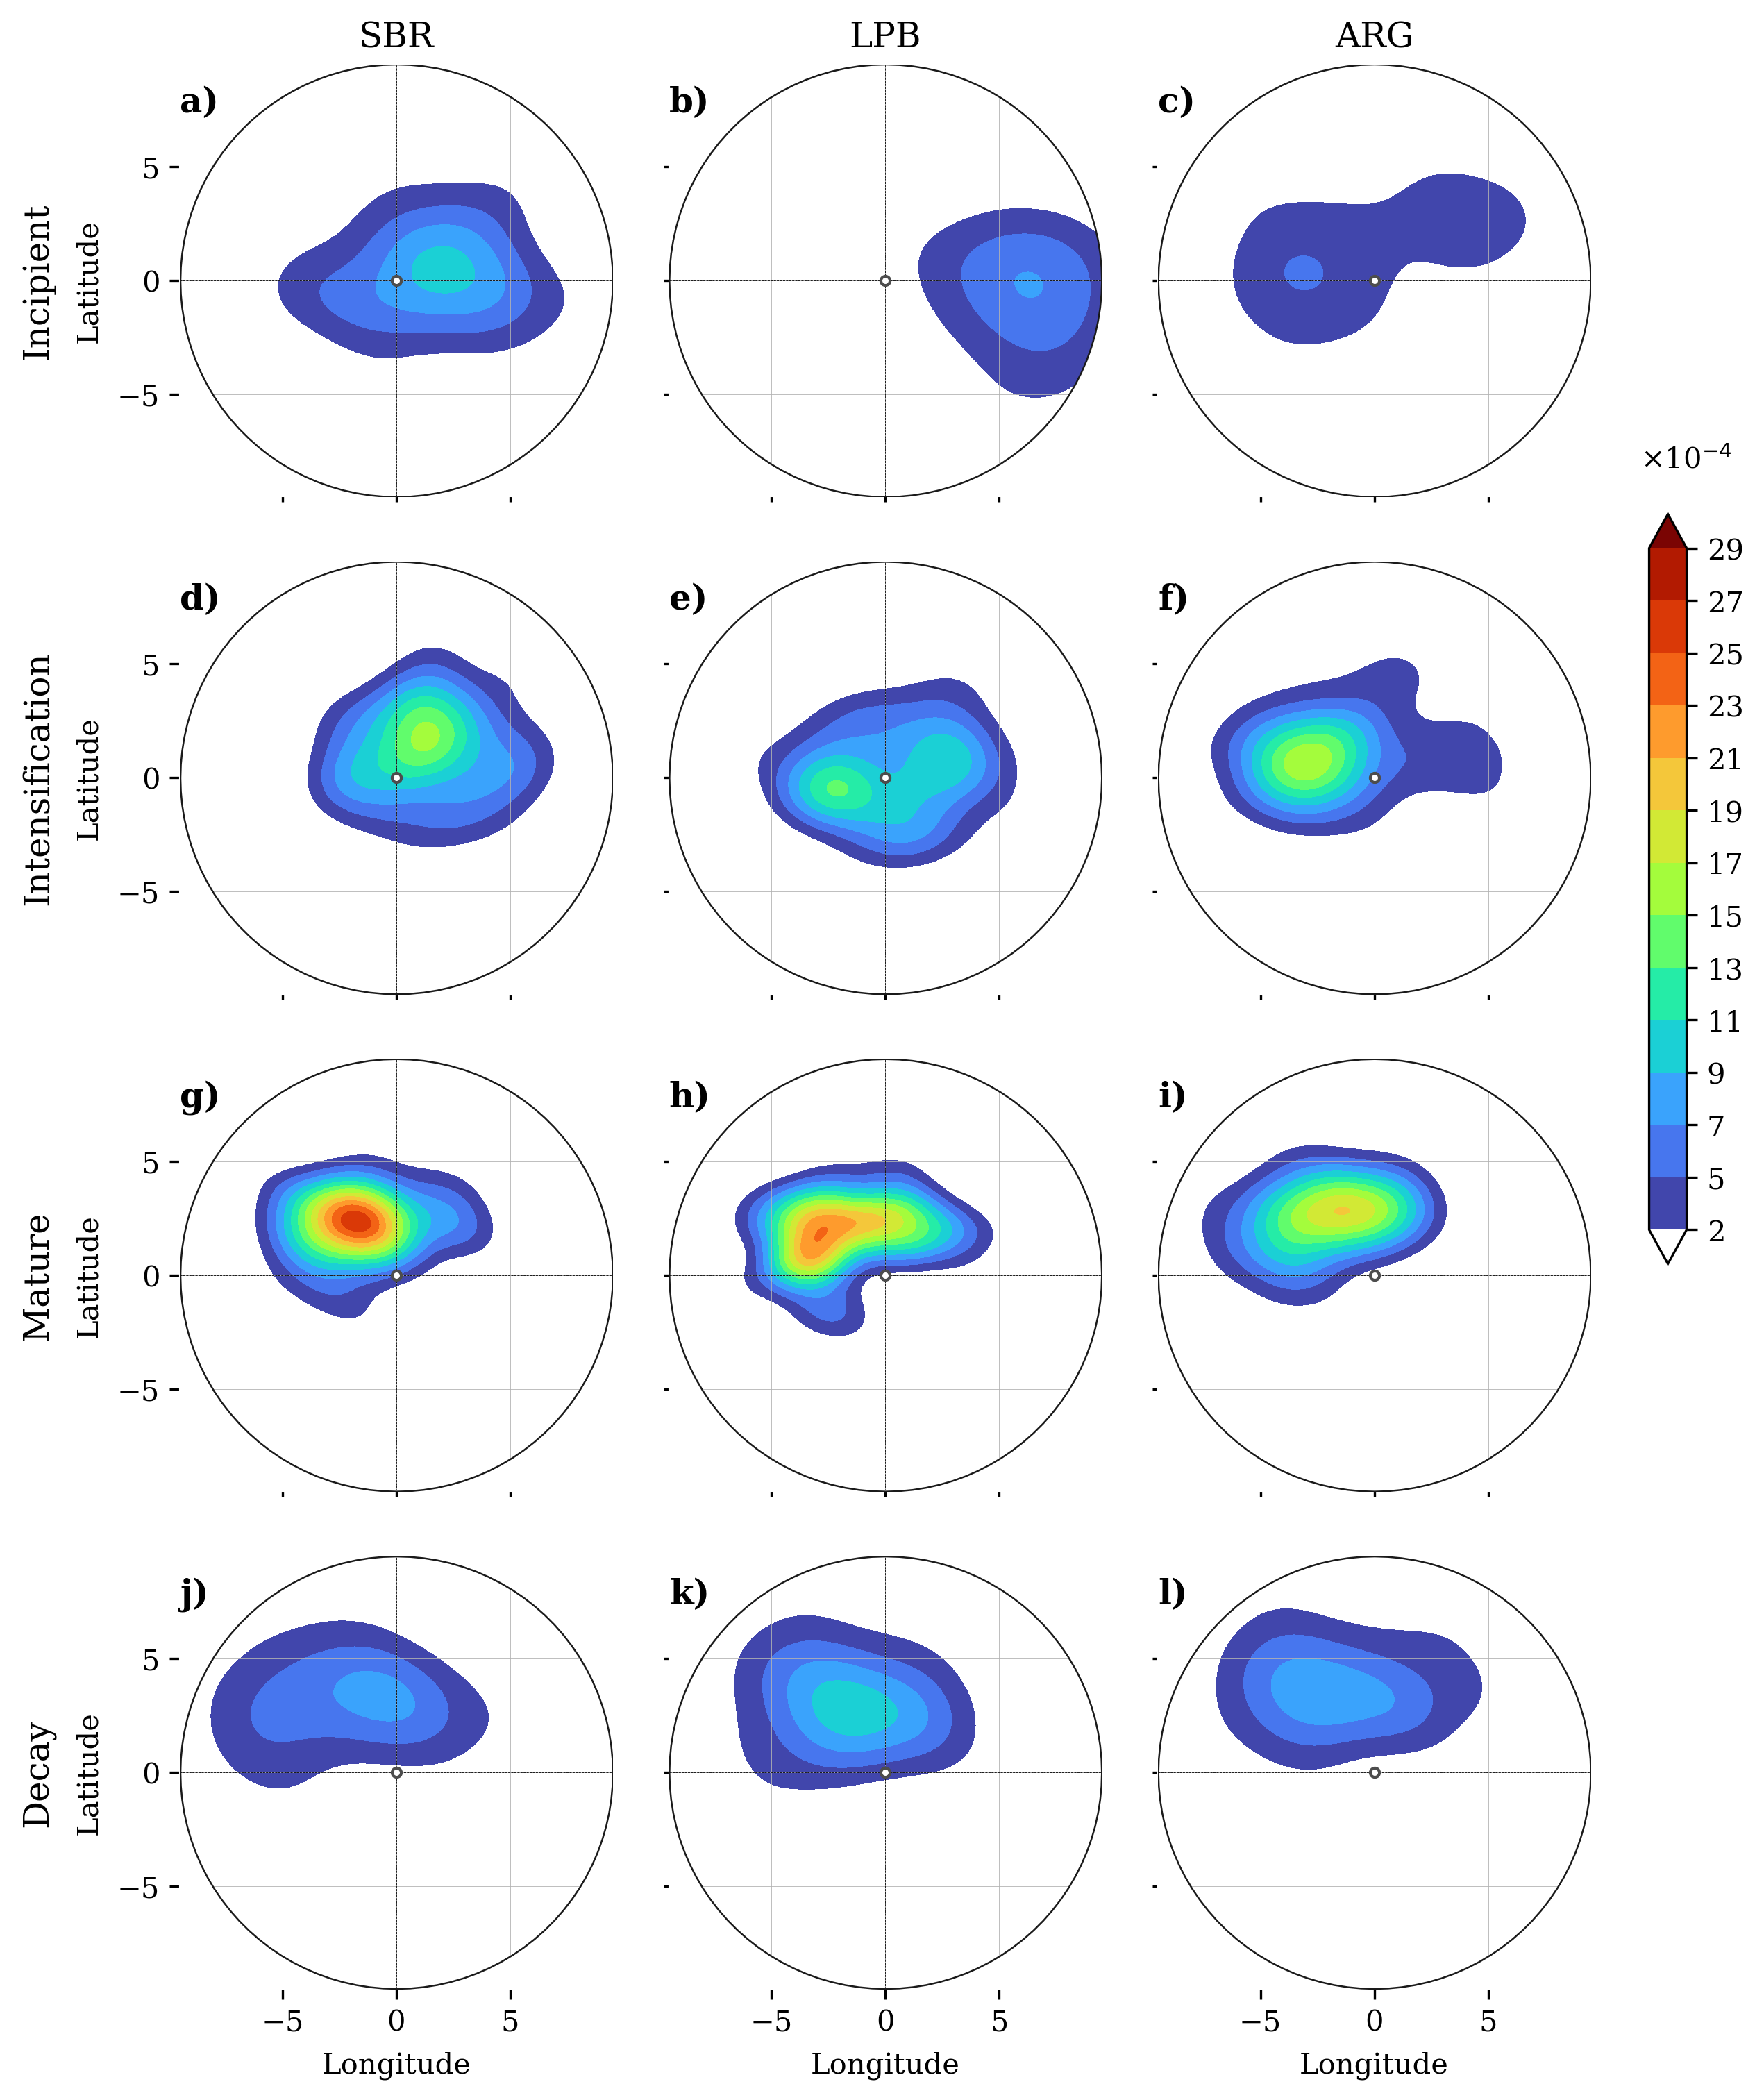
\includegraphics[width=\textwidth]{images/w10/kde_wind10_p90_fasesxreg.png}
\caption[PDF espacial de vento máximo a 10 metros (subconjunto p90)]{Estimação de densidade espacial bidimensional (PDFe; Seção~\ref{subsec:kde_localizacion}) da localização dos máximos de magnitude de vento a 10~metros para o subconjunto de ciclones intensos. O formato, domínio centrado no ciclone, fases evolutivas e escala de densidade ($10^{-4}$) são idênticos aos apresentados na Figura~\ref{fig:kde_wind_global} para permitir a comparação estrutural direta das assimetrias de densidade.}
\label{fig:kde_wind_p90}
\end{figure}

No subconjunto p90, a localização dos máximos se concentra progressivamente em um quadrante preferencial à medida que o ciclone evolui (Figura~\ref{fig:kde_wind_p90}).

Na fase incipiente (Ic; painéis a, b e~c), as três regiões apresentam densidades baixas e sem uma zona preferencial definida, de forma semelhante à População Global. Na intensificação (It; painéis d, e e~f), os núcleos começam a se deslocar para o oeste. Em SBR (d), o núcleo se localiza a nordeste e próximo do centro, mais a oeste do que na fase incipiente; em LPB (e), o núcleo principal se situa a oeste-sudoeste, com um núcleo secundário de menor densidade a leste; e em ARG (f), o núcleo se mantém a oeste do centro, como na fase incipiente, mas sua densidade aumenta de $5$--$7$ para $15$--$17\times10^{-4}$.
Na maturidade (M; painéis g, h e~i) forma-se um núcleo de alta densidade no quadrante noroeste, entre $-1^{\circ}$ e $-3^{\circ}$ de longitude e entre $+1.5^{\circ}$ e $+3^{\circ}$ de latitude em relação ao centro.
A densidade máxima é de 25--27\,$\times 10^{-4}$ em SBR (g), ${\approx}$\,23--25\,$\times 10^{-4}$ em LPB (h) e ${\approx}$\,19--21\,$\times 10^{-4}$ em ARG (i), cujo núcleo é menos compacto. Essa ordem regional não se repete na magnitude do vento (Seção~\ref{sec:pdf_wind10}), onde LPB e ARG apresentam os picos de densidade mais altos e SBR a distribuição mais larga, o que indica que a região que mais concentra a localização de seus máximos não é a que mais concentra sua intensidade.
No decaimento (D; painéis j, k e~l), o núcleo permanece no noroeste nas três regiões, enquanto na População Global o de SBR se localizava a leste-nordeste.

Essa alta concentração no noroeste é o traço espacial mais distintivo do vento nos ciclones p90 durante a maturidade, comum às três regiões de estudo.
Em ciclones do Hemisfério Norte documentam-se padrões análogos, com os ventos extremos associados ao \textit{sting jet}, que desce na zona de fratura frontal, e ao jato da cinta transportadora fria (CCB, \textit{cold conveyor belt}), situado abaixo e atrás dele \citep{clark2005sting, clark2018sting}, duas estruturas difíceis de distinguir em superfície por sua proximidade no espaço e no tempo \citep{eisenstein2023identification}. Pela inversão da circulação entre hemisférios, esse setor corresponde ao quadrante noroeste no Hemisfério Sul.
Com a mesma lógica, o máximo de vento que \citet{rudeva2011composite} localizam no setor sudoeste de ciclones do Atlântico Norte, a meia distância entre o centro e a borda do sistema, corresponderia ao quadrante noroeste no Hemisfério Sul, embora essa correspondência se baseie na simetria entre hemisférios e não em uma comparação direta.
De forma semelhante, \citet{priestley2022improved} situam os máximos do vento relativo ao sistema a 850~hPa associados ao CCB a ${\sim}$3--3.5$^{\circ}$ do centro e no flanco posterior de ciclones do Hemisfério Norte, uma distância comparável à do núcleo aqui identificado, e \citet{laurila2021characteristics} mostram que, nas tempestades de vento do norte da Europa, as rajadas mais intensas se deslocam do setor quente para detrás da frente fria ao longo da evolução do ciclone. Em um composto dos 100 ciclones mais intensos do Atlântico Norte, \citet{gentile2025response} descrevem uma sequência semelhante para o vento a 10~m, que se localiza no setor quente e em direção ao equador durante as primeiras etapas, e detrás do centro, no setor frio e ainda em direção ao equador, à medida que o ciclone se intensifica, o que no Hemisfério Sul corresponderia a um deslocamento para o noroeste.

No Atlântico Sul, \citet{gramcianinov2023impact} constatam que as ondas extremas associadas a ciclones ocorrem principalmente nos setores oeste e noroeste do ciclone, dominados pelo CCB, exceto em SBR durante o verão, quando predomina o setor leste, influenciado pelo WCB.
Em contraste, o composto de \citet{catto2010climate} sobre os 100 ciclones mais intensos do Hemisfério Norte no inverno situou parte dos ventos mais intensos a 925~hPa (${39.1 \pm 3.5}$~m\,s$^{-1}$, a ${5.1^{\circ} \pm 2.7^{\circ}}$ do centro) no setor quente onde se localiza o WCB, o que no Hemisfério Sul corresponderia ao quadrante nordeste. Essa diferença em relação ao núcleo noroeste de p90 poderia refletir o nível analisado (925~hPa contra 10~m) e o fato de que seu composto é construído no instante de máxima intensidade de cada ciclone, sem separar fases.
Fora do Atlântico Norte, a climatologia global de \citet{gray2024global}, que identifica precursores de \textit{sting jet} nos três oceanos durante 43 invernos, mostra que ciclones com esses precursores também ocorrem no Hemisfério Sul, embora com menor frequência (${\sim}$15\% do decil superior de intensidade, contra ${\sim}$27\% no Hemisfério Norte).

A concentração desse núcleo poderia estar relacionada ao transporte de momento em direção à superfície. Próximo à frente fria desenvolvem-se correntes descendentes que transportam momento horizontal de níveis altos para níveis baixos, e em climatologias do Hemisfério Norte essas correntes são cerca de 15\% mais frequentes no setor sudoeste do ciclone, que corresponde ao noroeste no Hemisfério Sul \citep{hyeok2024extrem}. Além disso, segundo \citet{martinez2014cold} (Seção~\ref{subsec:tb_modelos}), os ventos mais intensos na parte posterior do núcleo estão associados ao CCB e ao \textit{sting jet}, e o jato de baixo nível do CCB se intensifica pelo aumento de vorticidade potencial gerado pelo aquecimento diabático sob a ascensão do WCB \citep{schemm2014linkage}.

\citet{gentile2023observed} mostram também que, em ciclones maduros, o CCB ocorre no setor frio com camadas limite mais profundas e instáveis, o que favorece a mistura de ar de alta velocidade em direção à superfície e seria compatível com a concentração observada na PDFe. \citet{stankovic2025surface} reportam extremos de vento em superfície mais intensos no Hemisfério Norte do que no oceano Austral, associados a uma maior baroclinicidade em níveis médios, o que deve ser considerado ao comparar as magnitudes aqui obtidas com estudos desse hemisfério.

Deve-se considerar que o ERA5 pode subestimar a intensidade do vento por sua resolução. Ao não resolver explicitamente as estruturas de mesoescala, tende a subestimar as magnitudes extremas \citep{hodges2011comparison}, em torno de 10\% para o vento dos ciclones mais intensos segundo \citet{chen2024evaluation} (Seção~\ref{sec:datos_era5}), o que deve ser levado em conta ao interpretar os valores absolutos.

Uma referência observacional da magnitude que o vento pode alcançar nessas estruturas é o caso documentado por \citet{shapiro1990life}. Durante a fase de seclusão quente de um ETC profundo do Atlântico Norte (pressão central ${\sim}935$~hPa), medições de aeronave registraram velocidades de ${\sim}$40~m\,s$^{-1}$ a cerca de 300~m de altitude. Embora não correspondam ao vento a 10~m, que é menor por efeito do atrito, esses valores sugerem que as caudas de até 30~m\,s$^{-1}$ de p90 no ERA5 (Seção~\ref{sec:pdf_wind10}) poderiam estar subestimadas.

\citet{gray2020prototype} documentam um caso próximo à superfície, a tempestade Brendan (Reino Unido, janeiro de 2020; aprofundamento de 49~hPa em 24~h), no qual o dispersômetro ASCAT registrou ventos equivalentes a 10~m superiores a 55~nós (${\sim}28$~m\,s$^{-1}$) ao sul do centro, na zona de fratura frontal apontada como precursora de \textit{sting jet}, embora nessas observações o CCB e o \textit{sting jet} não possam ser distinguidos. Pela inversão entre hemisférios, essa zona corresponde ao lado norte do centro no Hemisfério Sul, e a magnitude registrada é comparável às caudas de p90 aqui obtidas.

Em conjunto, esses resultados mostram que a intensidade de um ciclone está associada ao seu padrão espacial. Os ciclones intensos das três regiões tendem a concentrar seus máximos de vento a 10~m a uma distância e em um quadrante preferenciais em relação ao centro, o que sugere incorporar a localização, e não apenas a magnitude, ao avaliar os impactos do vento associados a esses sistemas.
%%%%%%%%%%%%%
% --- SEÇÃO: PADRÕES DOMINANTES DE VARIABILIDADE (EOF) - VENTO A 10 METROS,
\section{Organização estrutural: Análise EOF}\label{sec:eof_wind10}
\subsection{Fracionamento de variância}\label{sec:var_exp_wind10}
\begin{figure}[htbp]
\centering
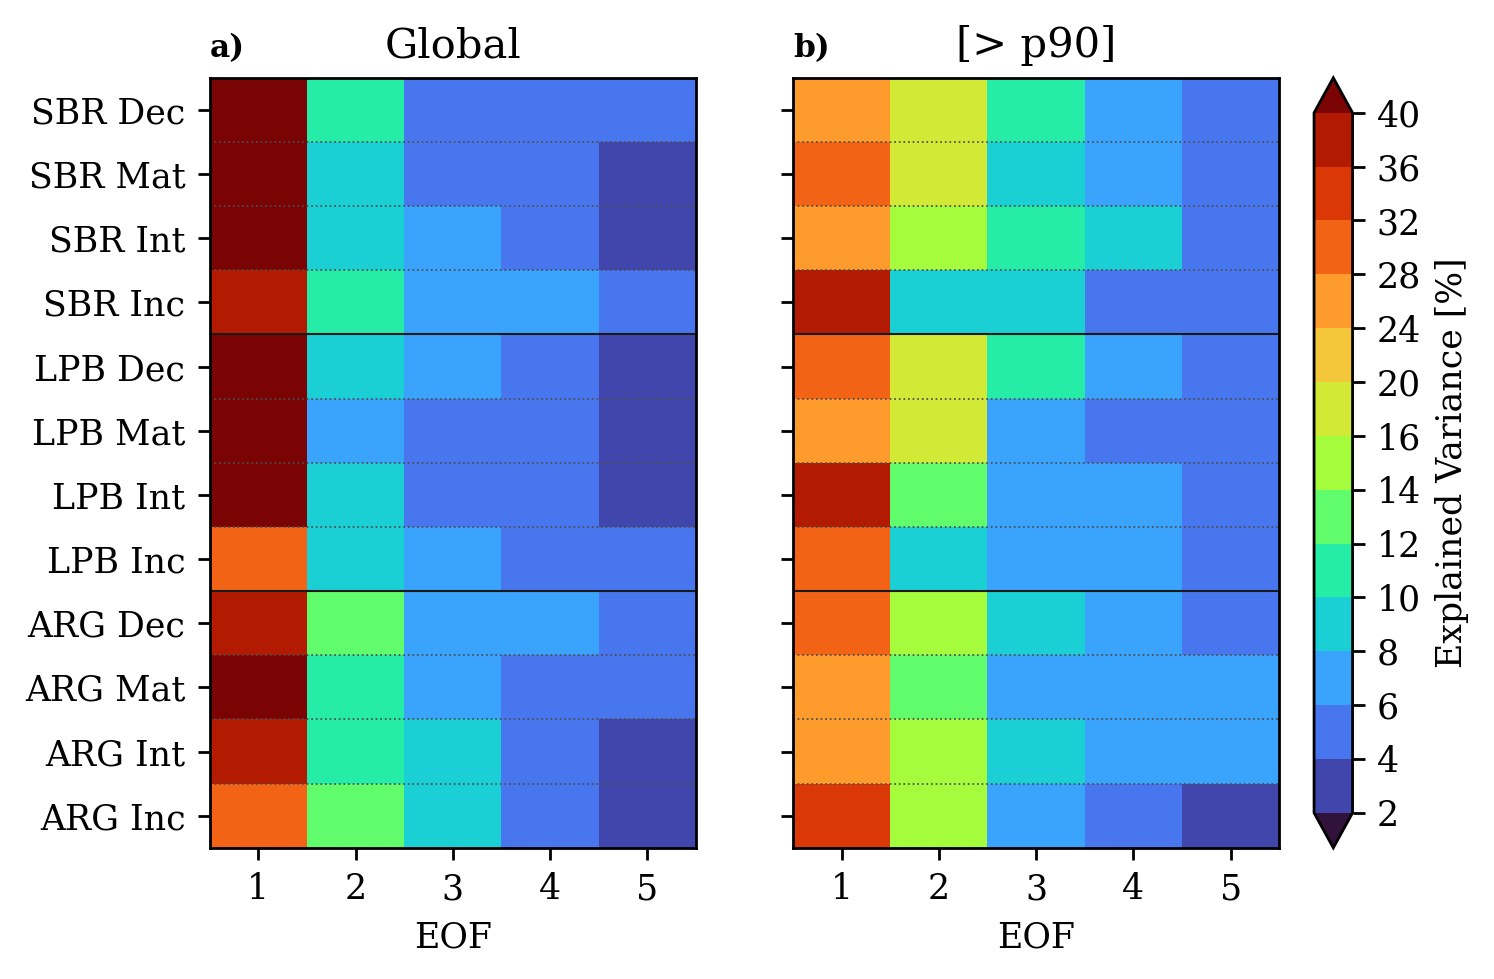
\includegraphics[width=0.8\textwidth]{images/w10/all_expvar_wind10_mean2times.png}
\caption[Variância explicada pelos primeiros cinco modos (EOF1--EOF5) de vento a 10~m]{Fracionamento da variância espacial total contida nos primeiros cinco modos dominantes (EOF1 a EOF5) do vento a 10~metros, obtida mediante o procedimento descrito na Seção~\ref{subsec:eof_univariado}. Contrasta-se a distribuição da variância da População Global com o subconjunto de intensidade p90 ao longo do ciclo de vida para cada região de ciclogênese.}
\label{fig:var_exp_wind10}
\end{figure}

A Figura~\ref{fig:var_exp_wind10} resume a variância explicada pelos cinco primeiros modos (EOF1 a EOF5) na População Global (painel~a) e em p90 (painel~b). Na População Global, EOF1 domina sobre os modos secundários em todas as regiões e fases, com valores máximos na maturidade (57.4\% em SBR e 57.1\% em LPB) e uma queda abrupta em direção ao EOF2. Os valores mais baixos são registrados em ARG (entre 30.9\% e 43.3\%) e em LPB durante a fase incipiente (31.9\%). Isso indica que, na População Global, a variabilidade do vento em superfície se concentra em um único padrão espacial, compatível com um gradiente de grande escala como o fluxo sinótico de fundo (Seção~\ref{subsec:eof_univariado}).

Em p90, EOF1 não supera 37.6\% em nenhuma região nem fase, com um mínimo de 25.4\% em ARG durante a intensificação, e a variância se distribui entre vários modos, com maior peso de EOF2 e EOF3. Segundo \citet{hannachi2007empirical}, o espectro de autovalores indica como a variância se distribui segundo a escala espacial, e quando os autovalores são próximos, os padrões correspondentes podem se misturar e devem ser interpretados com cautela. Nos ciclones intensos, a maior complexidade do vórtice, com frentes mais marcadas, jatos de baixo nível e seclusão quente (Seção~\ref{subsec:tb_modelos}), poderia explicar que sejam necessários vários modos (EOF2--EOF5) para representar a variabilidade do campo.

Esses resultados indicam que um ciclone intenso não é uma versão amplificada de um ciclone ordinário. Como em p90 a variância se distribui entre vários modos, descrever seus ventos a partir dos padrões da população média poderia não representar adequadamente a assimetria nem a localização de seus máximos.
%%%%%%%
\subsection{EOF1 na População Global}\label{subsec:eof1_wind10_global}

\begin{figure}[htbp]
\centering
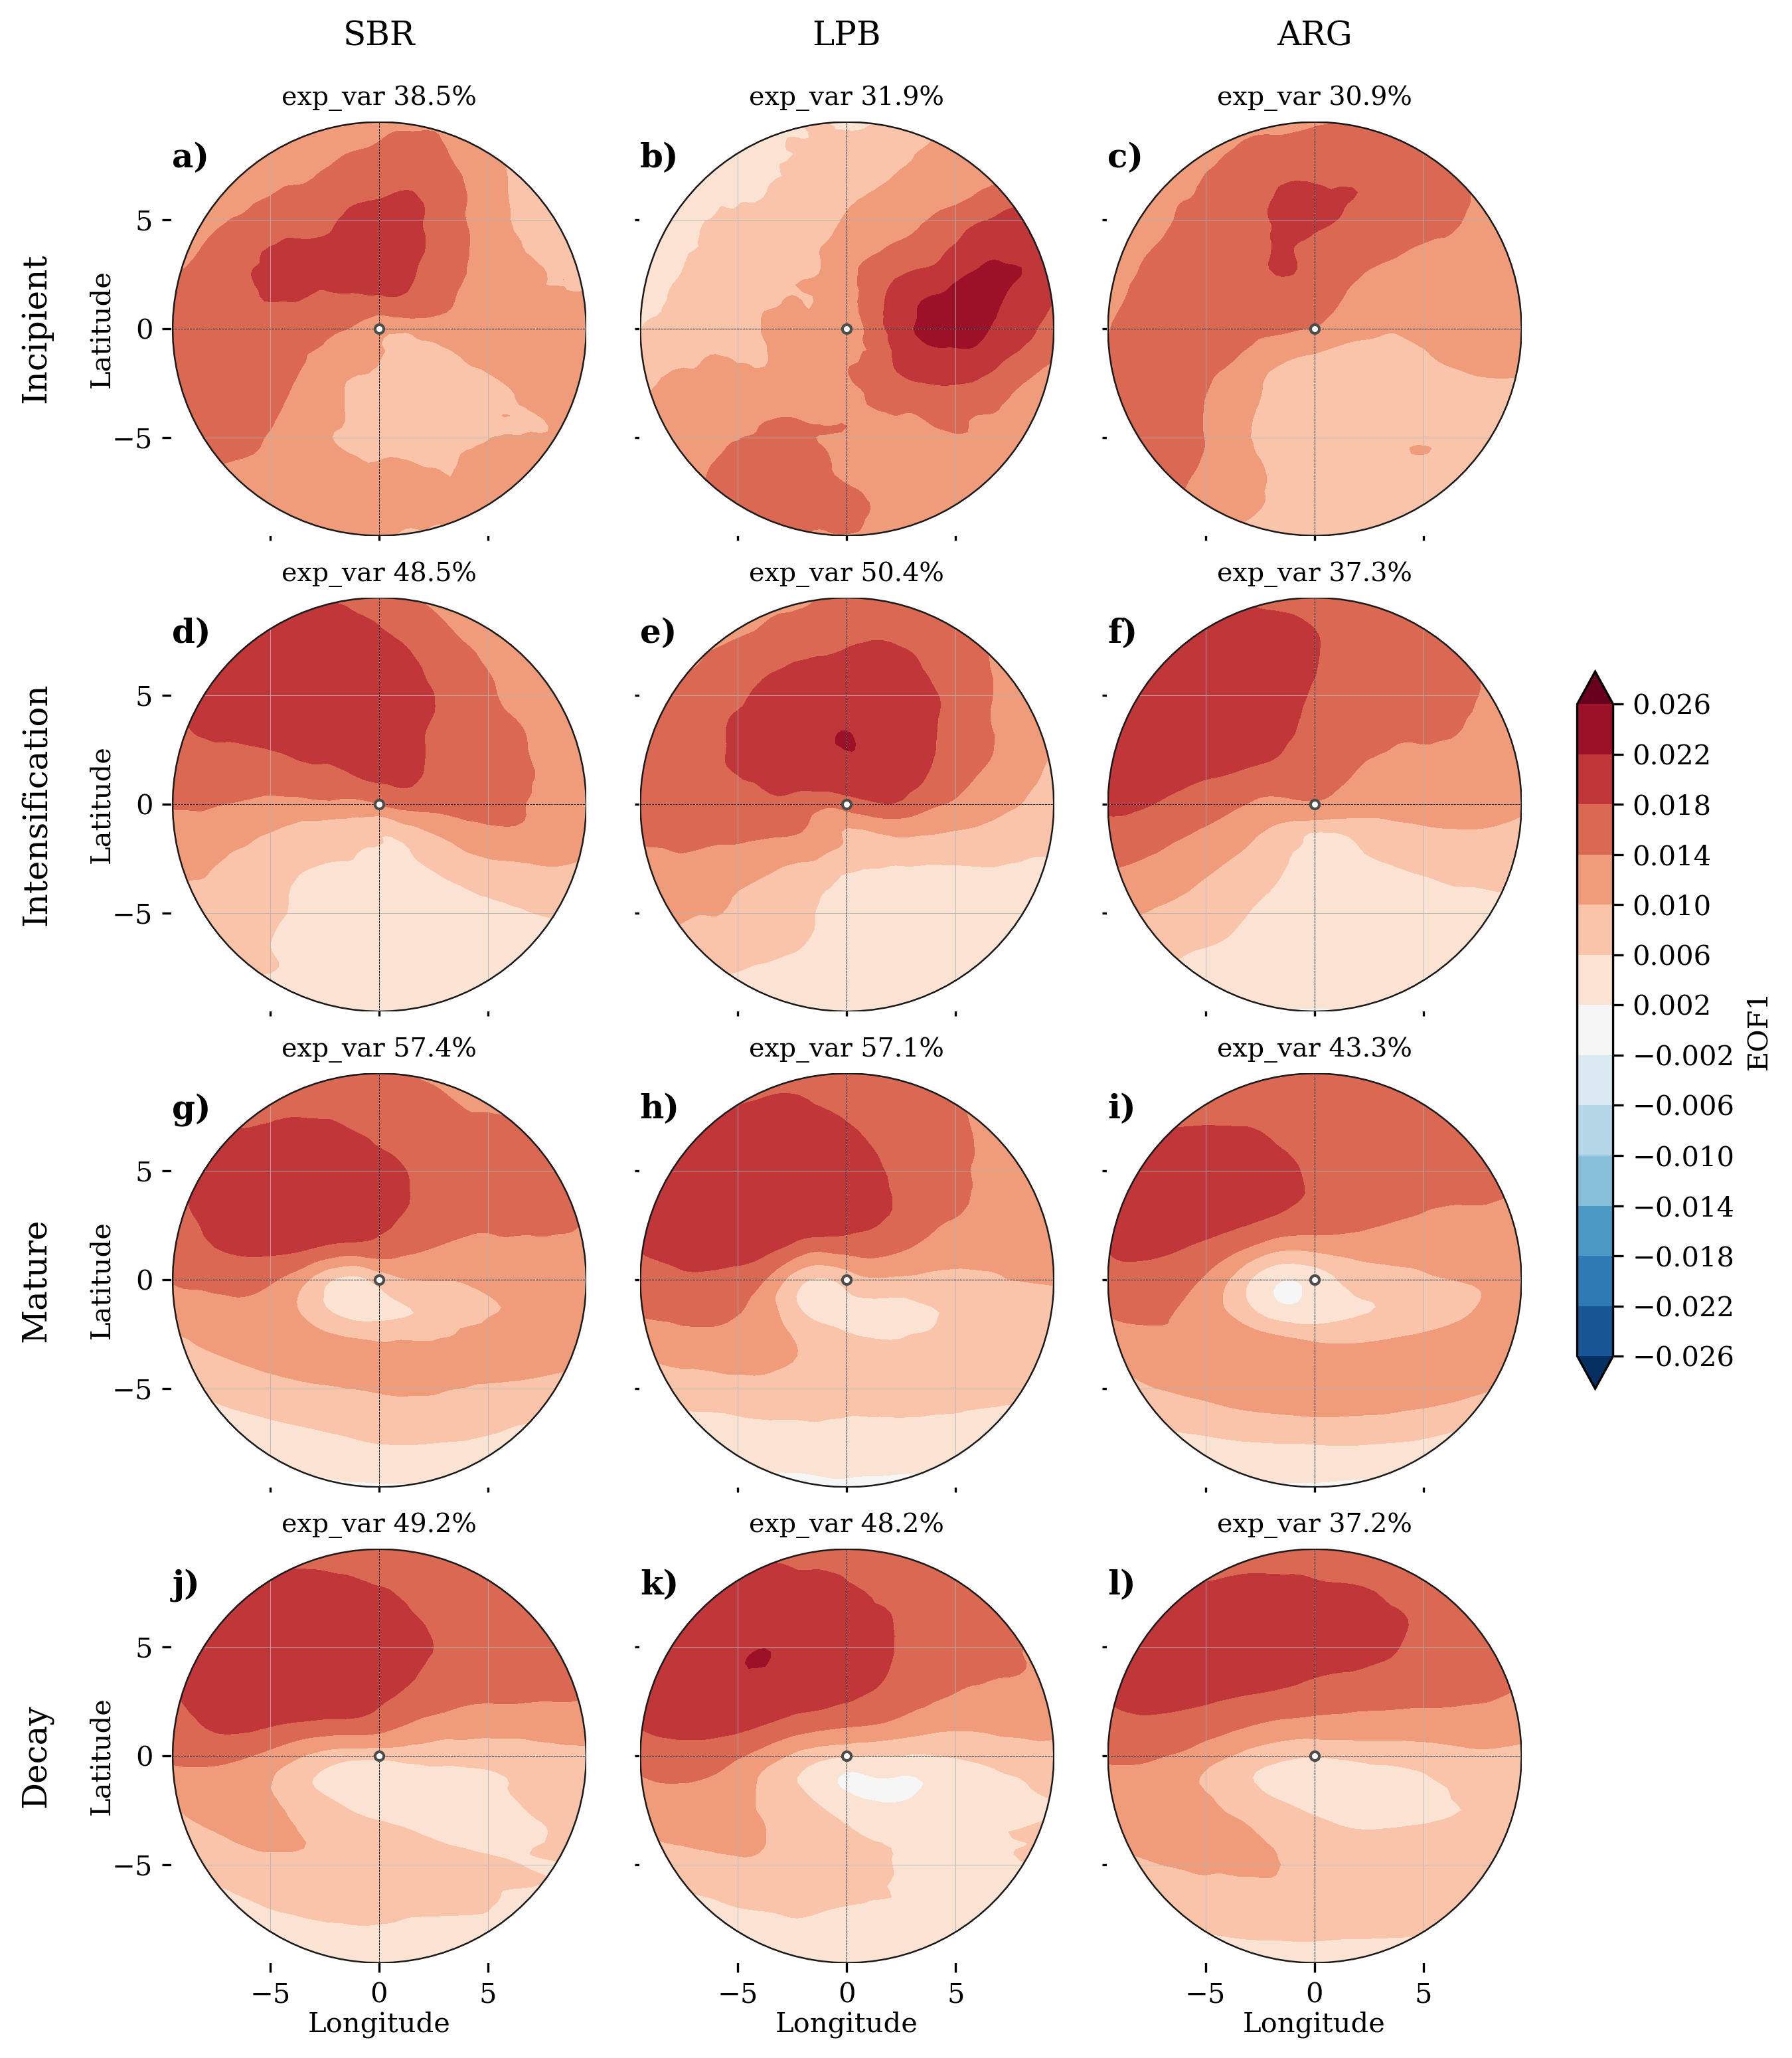
\includegraphics[width=\textwidth]{images/w10/pca1_wind10_global_fasesxreg.png}
\caption[EOF1 da magnitude do vento a 10 metros (População Global)]{Primeiro modo espacial (EOF1) da magnitude do vento a 10~metros para a População Global de referência, derivado da análise descrita na Seção~\ref{subsec:eof_univariado}. Os painéis (a--c) correspondem à fase incipiente (Ic) para as regiões SBR, LPB e ARG, respectivamente; (d--f) à intensificação (It); (g--i) à maturidade (M); e (j--l) ao decaimento (D). O título de cada painel indica o percentual de variância explicada (\textit{exp\_var}) por esse modo dominante. As cores quentes (frias) representam anomalias positivas (negativas) da estrutura do vento relativo ao centro do ciclone em um domínio de $20^{\circ} \times 20^{\circ}$.}
\label{fig:eof1_wind10_global}
\end{figure}

A Figura~\ref{fig:eof1_wind10_global} apresenta o EOF1 do vento a 10~m no domínio centrado no ciclone, que explica entre 30.9\% (ARG incipiente) e 57.4\% (SBR maturidade) da variância (Seção~\ref{sec:var_exp_wind10}). O padrão é positivo em todo o domínio e forma um gradiente norte--sul de grande escala, com valores altos no setor norte ($+0.010$ a $+0.026$) e valores próximos de zero no sul e em torno do centro. Esse gradiente se define progressivamente desde a fase incipiente até a maturidade, quando alcança sua maior variância explicada em SBR (g, 57.4\%) e LPB (h, 57.1\%). LPB se desvia desse comportamento nas primeiras fases, com o núcleo positivo a leste do centro na fase incipiente (b) e próximo do centro na intensificação (e). No decaimento (j, k e~l), as três regiões apresentam valores altos a noroeste que diminuem em direção ao sudeste, com anomalias positivas fracas em quase todo o domínio.

A presença desse gradiente norte--sul desde a intensificação até a maturidade, junto com sua alta variância explicada, sugere que a variabilidade do vento nos ciclones depende em parte de sua interação com o fluxo zonal de fundo e com as variações do gradiente latitudinal de temperatura.
Em LPB, onde o padrão se desvia desse comportamento nas primeiras fases, \citet{gramcianinov2019properties} apontam que o desenvolvimento inicial é influenciado por uma baixa orográfica, o que poderia manter a variabilidade do vento próxima do centro e retardar o surgimento do gradiente norte--sul.

No decaimento, a circulação ciclônica se debilita e a variabilidade do vento passa a depender principalmente do fluxo zonal do entorno.
Esse padrão estabelece a referência de variabilidade do vento nos ETC para a comparação com os ciclones intensos e com a análise multivariada (Seção~\ref{sec:meof_prototipos}).
%%%%%%
\subsection{EOF1 no subconjunto p90}\label{subsec:eof1_wind10_p90}

\begin{figure}[htbp]
\centering
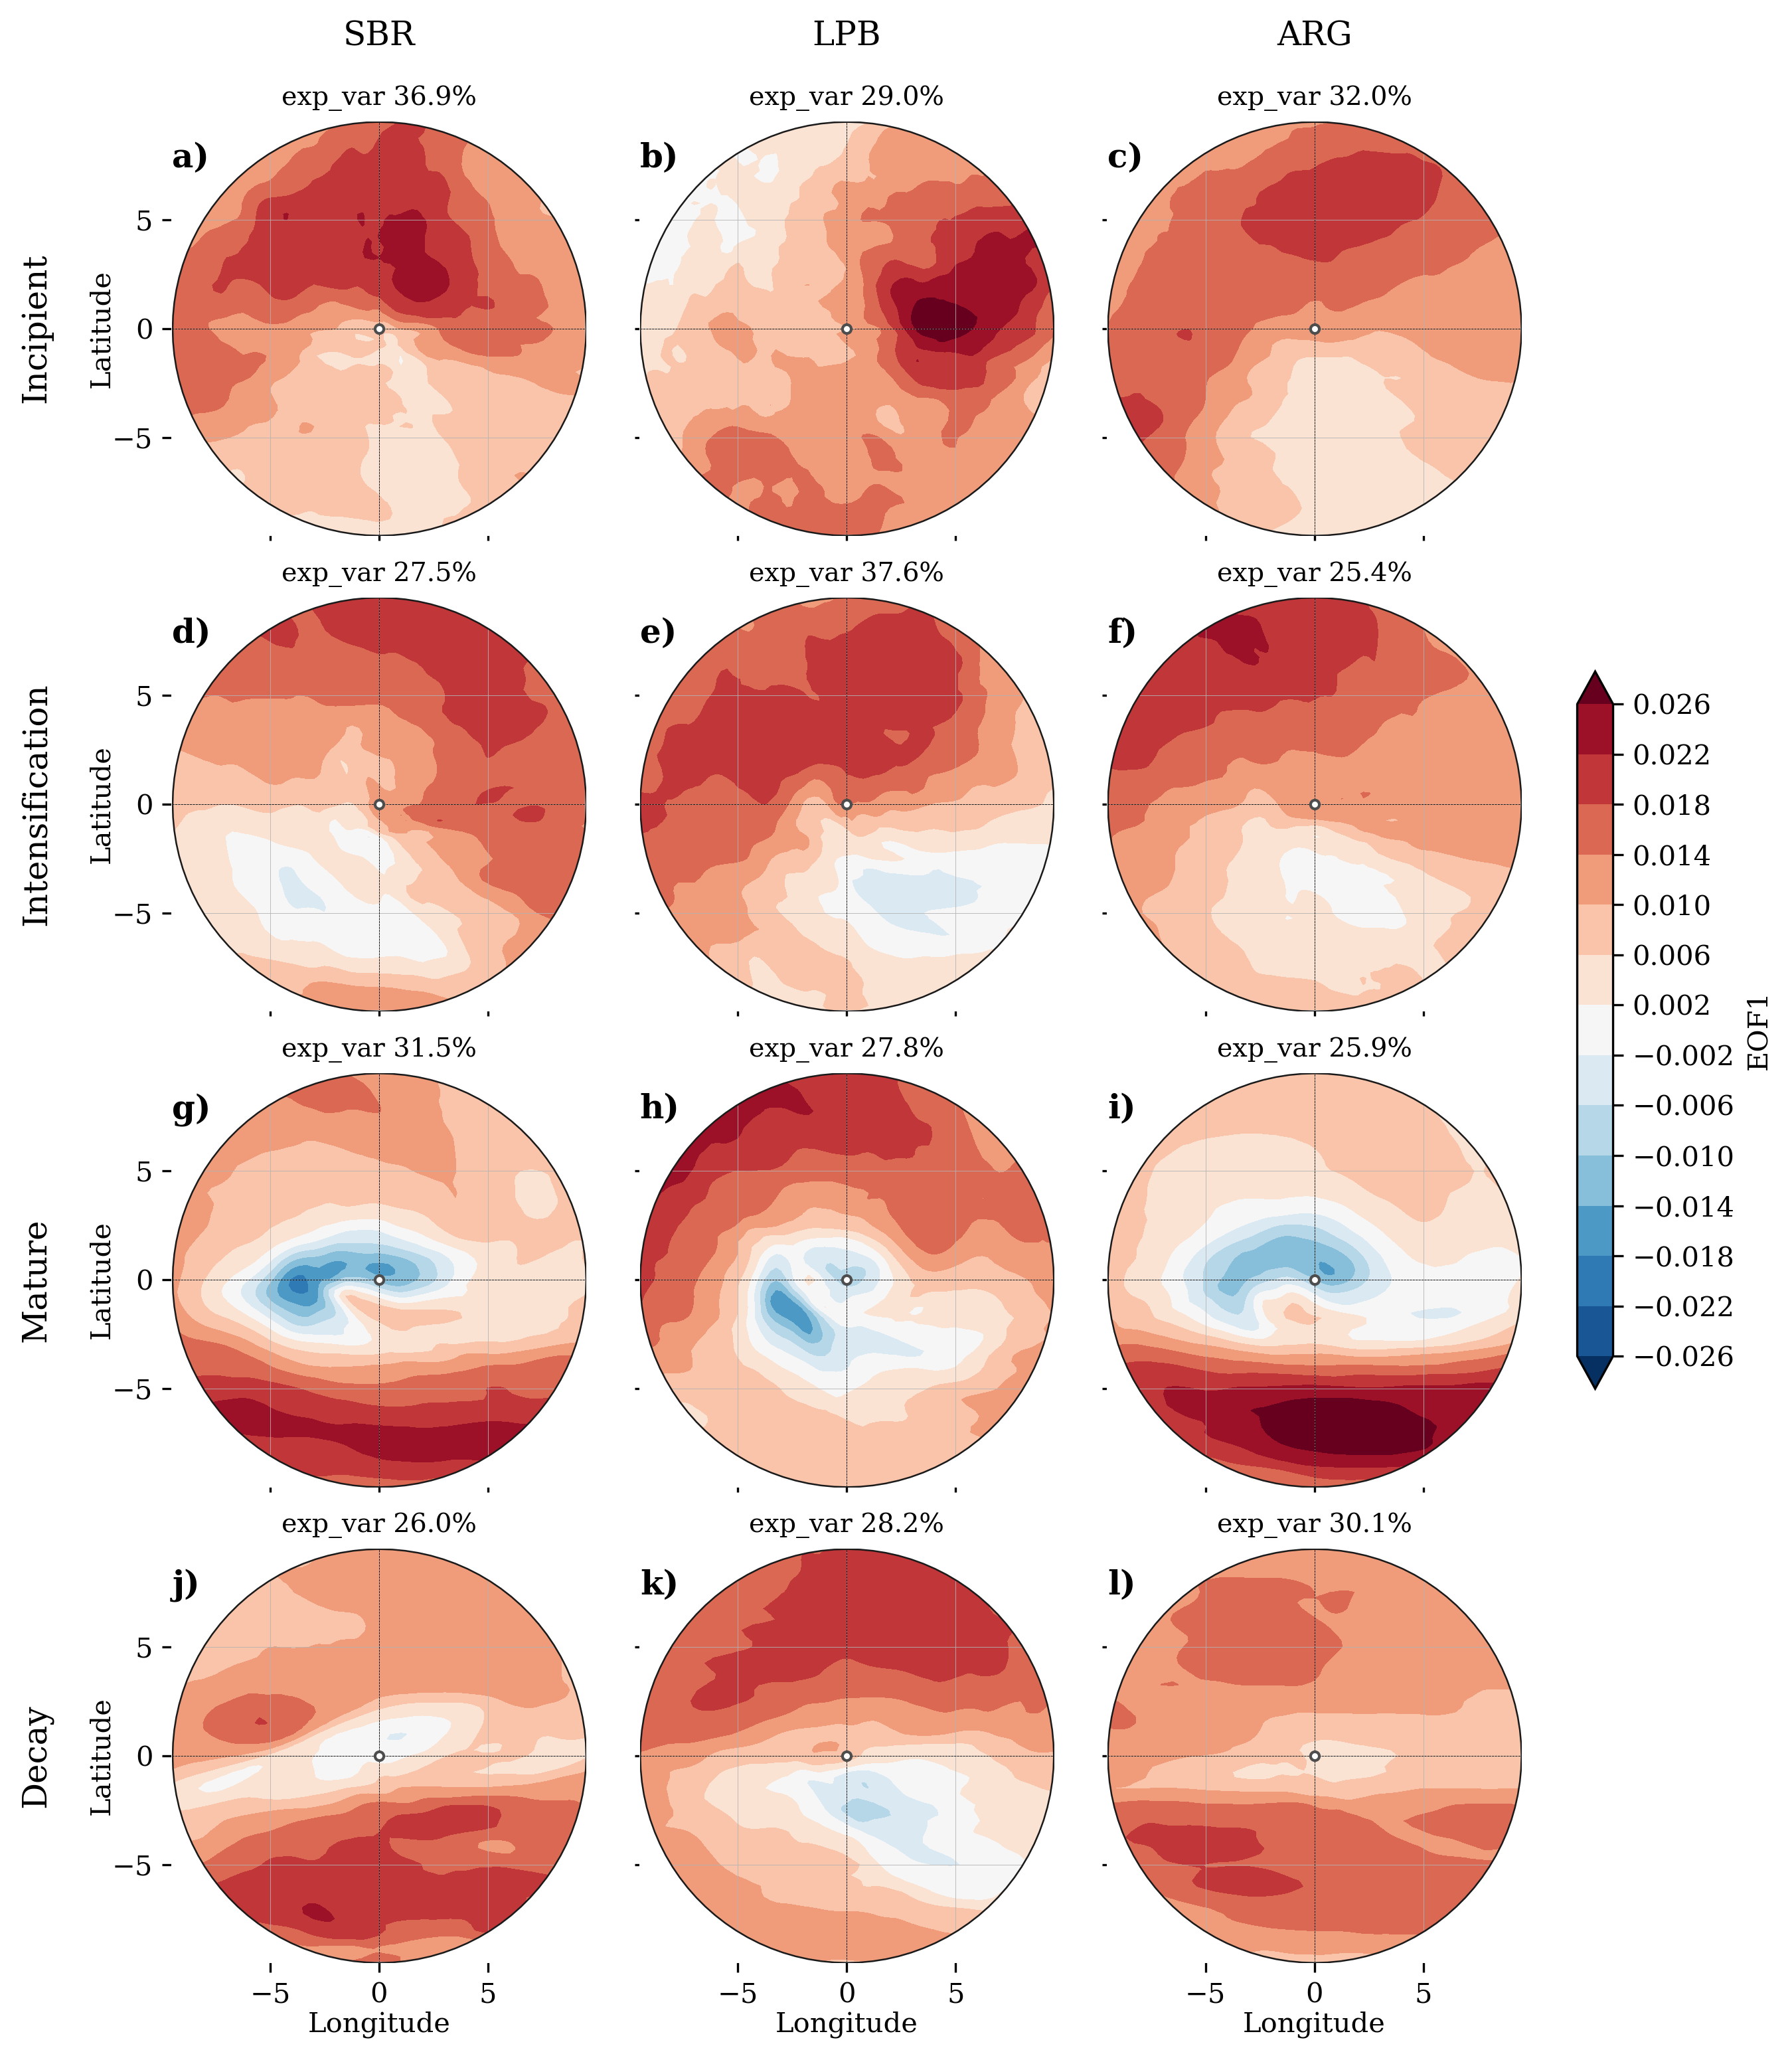
\includegraphics[width=\textwidth]{images/w10/pca1_wind10_p90_fasesxreg.png}
\caption[EOF1 da magnitude do vento a 10 metros (subconjunto p90)]{Primeiro modo espacial (EOF1) da magnitude do vento a 10~metros para o subconjunto de ciclones intensos (p90). A disposição dos painéis (a--l) por região de ciclogênese (colunas) e fase evolutiva (linhas) é idêntica à
Figura~\ref{fig:eof1_wind10_global}. Detalha-se a variância explicada (\textit{exp\_var}) em cada painel e a barra de cor padronizada para avaliar
as diferenças nos padrões espaciais dos ciclones intensos em relação à População Global.}
\label{fig:eof1_wind10_p90}
\end{figure}

Em p90, o EOF1 não amplifica o padrão da População Global, mas muda de forma. Sua variância explicada é menor (25.4--37.6\%) e o padrão apresenta estruturas mais localizadas do que o gradiente norte--sul de grande escala da Seção~\ref{subsec:eof1_wind10_global}.

Na fase incipiente (a, b e~c), as três regiões mostram padrões difusos, com anomalias positivas ao norte e nordeste e sem uma estrutura definida. Na intensificação (d, e e~f) aparece um gradiente norte--sul mais definido, com anomalias positivas ao norte, nordeste e noroeste e valores negativos fracos ao sul em SBR e LPB. ARG (f) apresenta os valores mais altos ($>+0.022$ no noroeste). A maior mudança ocorre na maturidade (g, h e~i), quando as três regiões desenvolvem um núcleo negativo compacto próximo do centro, rodeado de anomalias positivas ao norte e ao sul. Esse núcleo alcança valores de até $-0.022$ em SBR (g), a oeste do centro, e em LPB (h), onde se estende para o sudoeste, enquanto em ARG (i) é mais fraco. No decaimento (j, k e~l), o padrão perde definição e o domínio volta a ser majoritariamente positivo, com gradientes mais suaves, e apenas LPB mantém valores negativos fracos ao sul do centro.

Na maturidade, as anomalias se concentram próximo do núcleo, o que concorda com a distribuição da variância entre vários modos (Seção~\ref{sec:var_exp_wind10}). Nesses ciclones, o EOF1 deixa de descrever um gradiente sinótico extenso e passa a descrever a variabilidade próximo do núcleo, em posição e intensidade, o que sugere um maior peso da circulação de mesoescala em relação ao fluxo de fundo. Essa localização coincide com a zona onde a literatura situa o CCB e a fratura frontal (Seção~\ref{sec:kde_espacial_p90}), embora com o vento escalar disponível não seja possível distingui-la de outros mecanismos de escala semelhante, como o \textit{sting jet} ou a intrusão seca.

Em ARG durante a maturidade (i), as anomalias negativas em torno do centro são moderadas e a faixa positiva ao sul alcança os valores mais altos do domínio, padrão que poderia estar relacionado à seclusão quente (\textit{warm seclusion}; Seções~\ref{subsec:tb_modelos} e~\ref{subsec:tb_fases}).

Em conjunto, um ciclone intenso não é estruturalmente equivalente a um ciclone ordinário, já que sua dinâmica modifica a forma dos padrões de vento. Como apontam \citet{corner2025classification} e \citet{eisenstein2023identification}, a intensidade do vento em superfície não depende apenas da escala sinótica, mas também das estruturas de mesoescala.
%%%%%%%%
\subsection{Significância estatística}\label{subsec:res_significancia_madurez}

Para distinguir os sinais físicos das flutuações devidas à amostragem, avalia-se a significância estatística dos padrões espaciais mediante o método Bootstrap-t (Seção~\ref{subsec:bootstrap_significancia}), seguindo \citet{hesterberg2015bootstrap}. A análise se concentra na fase de maturidade, que apresenta o maior sinal dinâmico e é a de maior interesse para esta tese. A Figura~\ref{fig:xeof_madurez_global} mostra os três primeiros modos (EOF1--EOF3) e suas componentes principais (PC1--PC3) para a População Global na maturidade, e a Figura~\ref{fig:xeof_madurez_p90} apresenta a análise equivalente para p90. O hachurado indica as áreas significativas a 95\% de confiança.

\begin{figure}[htbp]
\centering
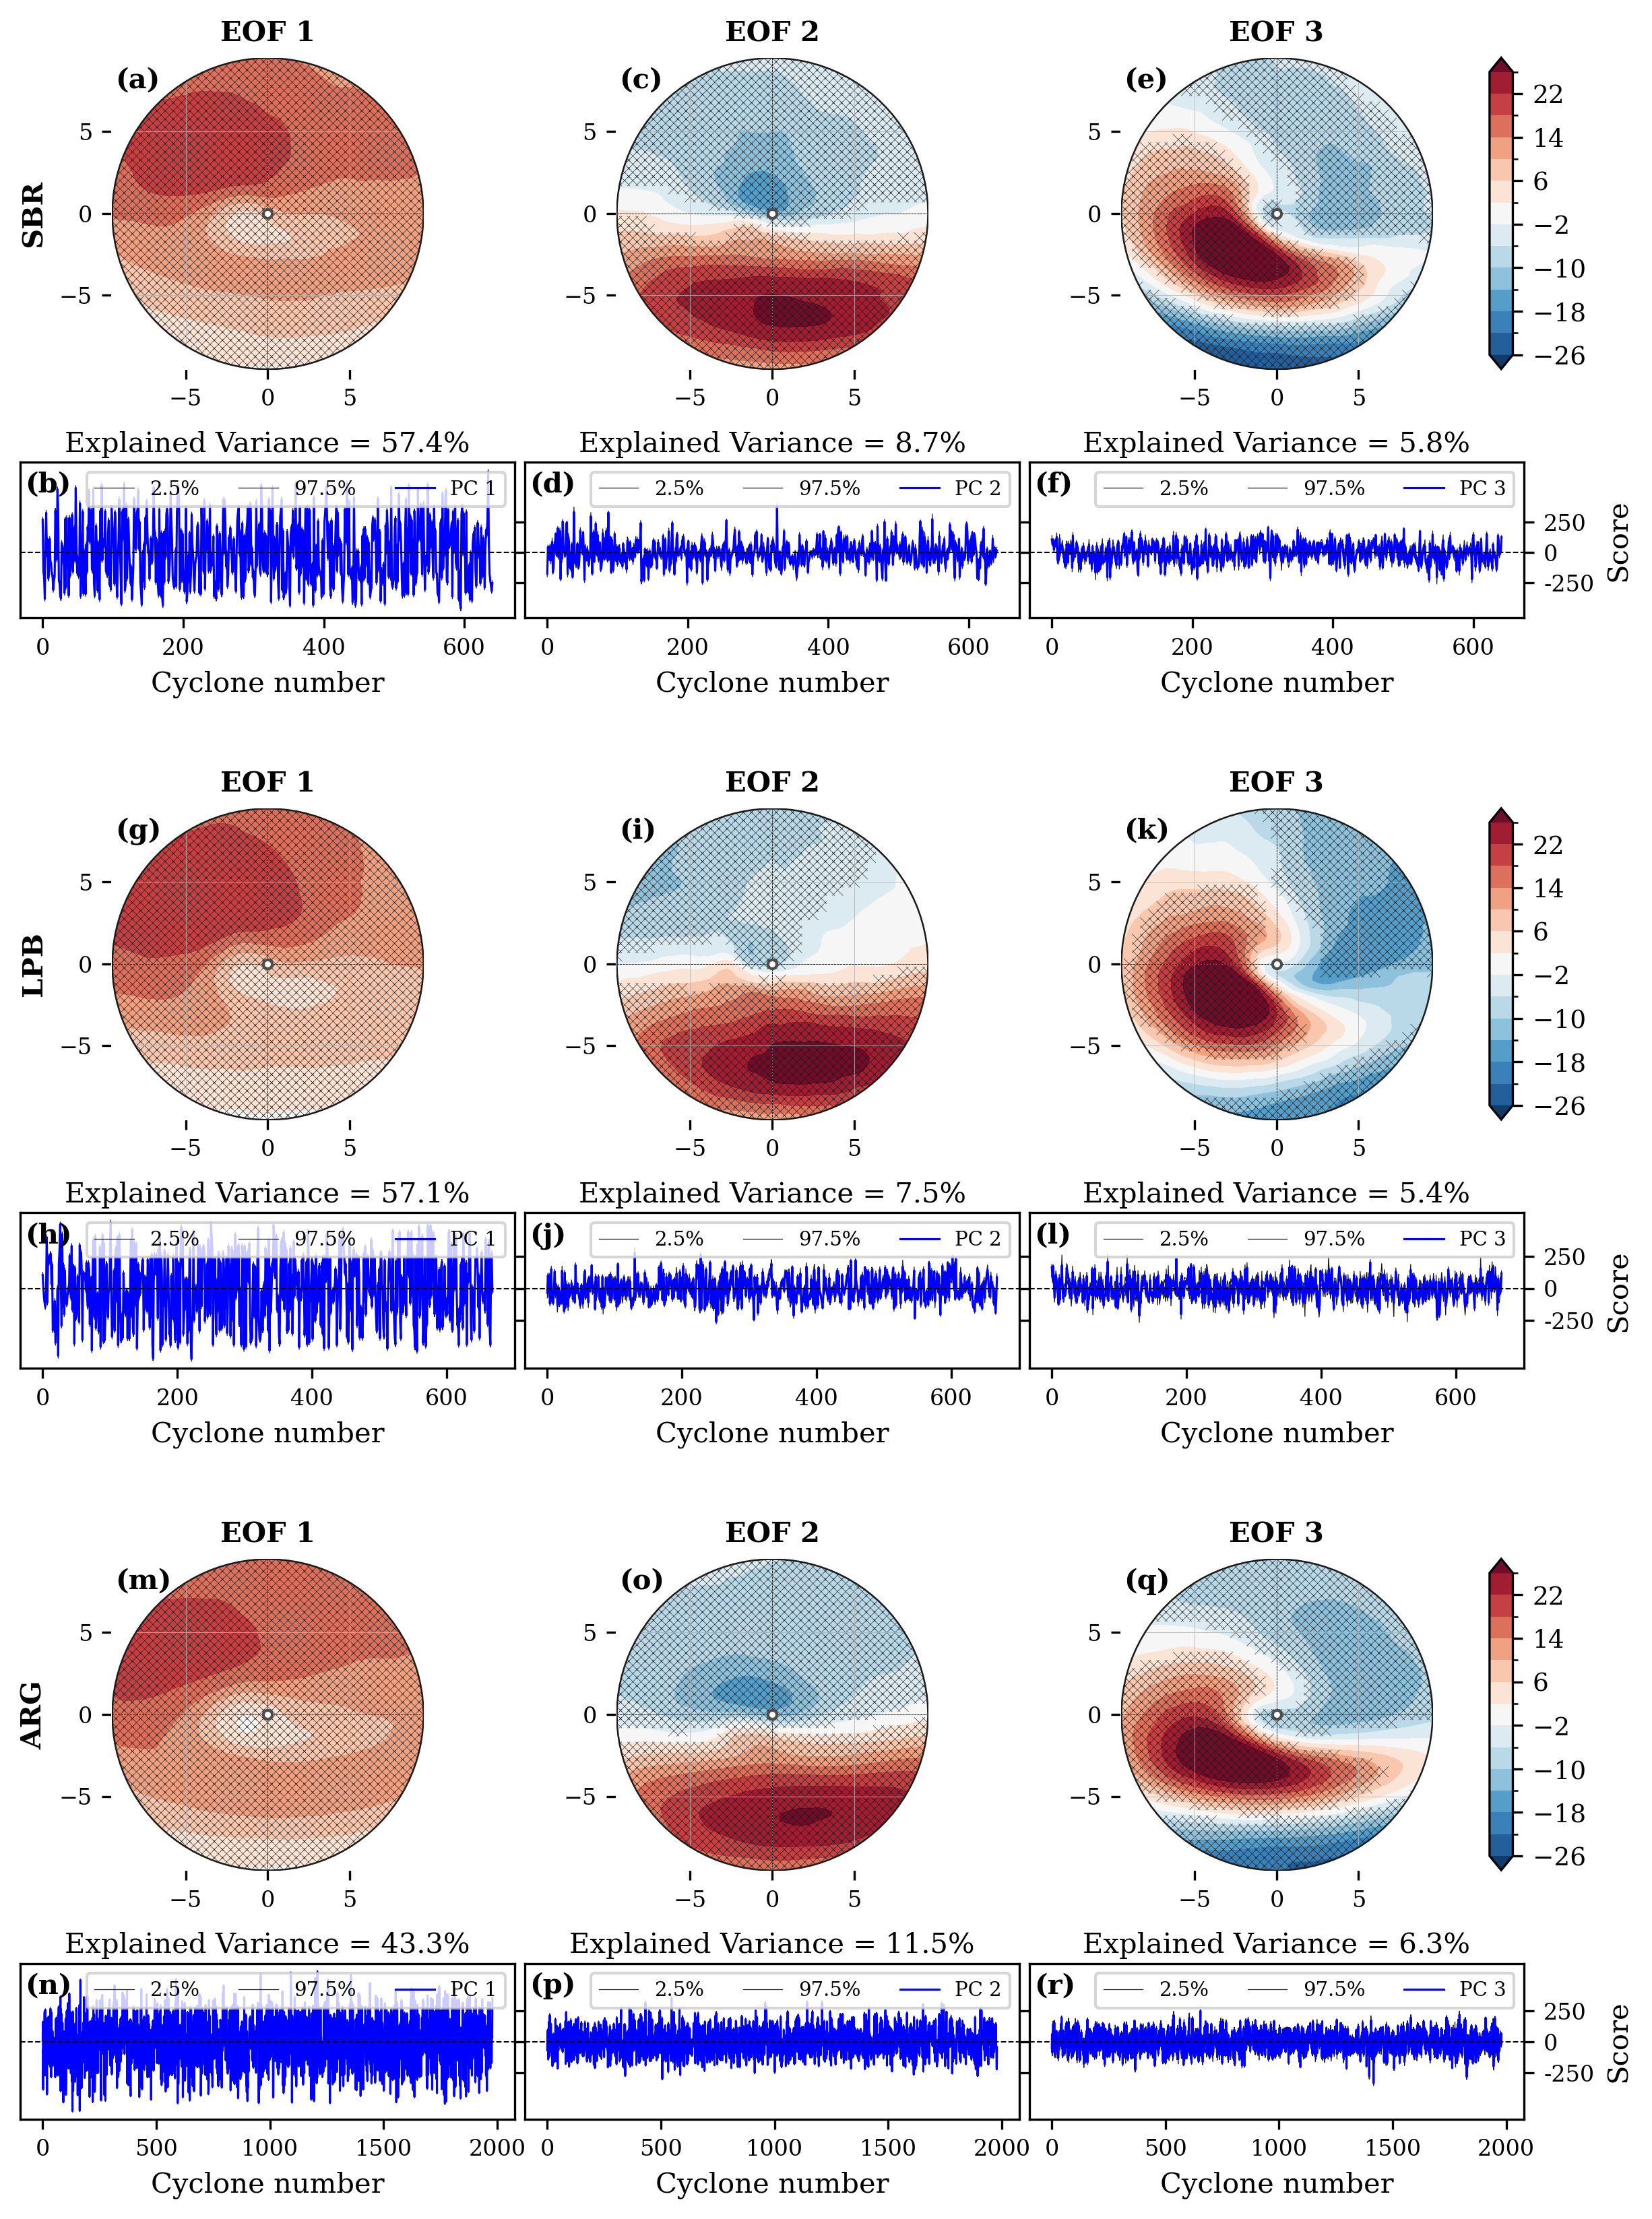
\includegraphics[width=\textwidth]{images/w10/xeof_global_wind10_mature.png}
\caption[Significância espacial dos EOFs em fase de maturidade (População Global)]{Decomposição EOF do vento a 10~m para a População Global em fase de maturidade. Painéis (a, g, m): mapas de EOF1 para SBR, LPB e ARG respectivamente; (c, i, o): EOF2; (e, k, q): EOF3. O hachurado indica significância estatística a 95\% (teste Bootstrap-t; Seção~\ref{subsec:bootstrap_significancia}). Painéis (b, h, n): componentes principais PC1; (d, j, p): PC2; (f, l, r): PC3. A linha cinza delimita os percentis 2.5 e 97.5 da distribuição bootstrap.}
\label{fig:xeof_madurez_global}
\end{figure}

\begin{figure}[htbp]
\centering
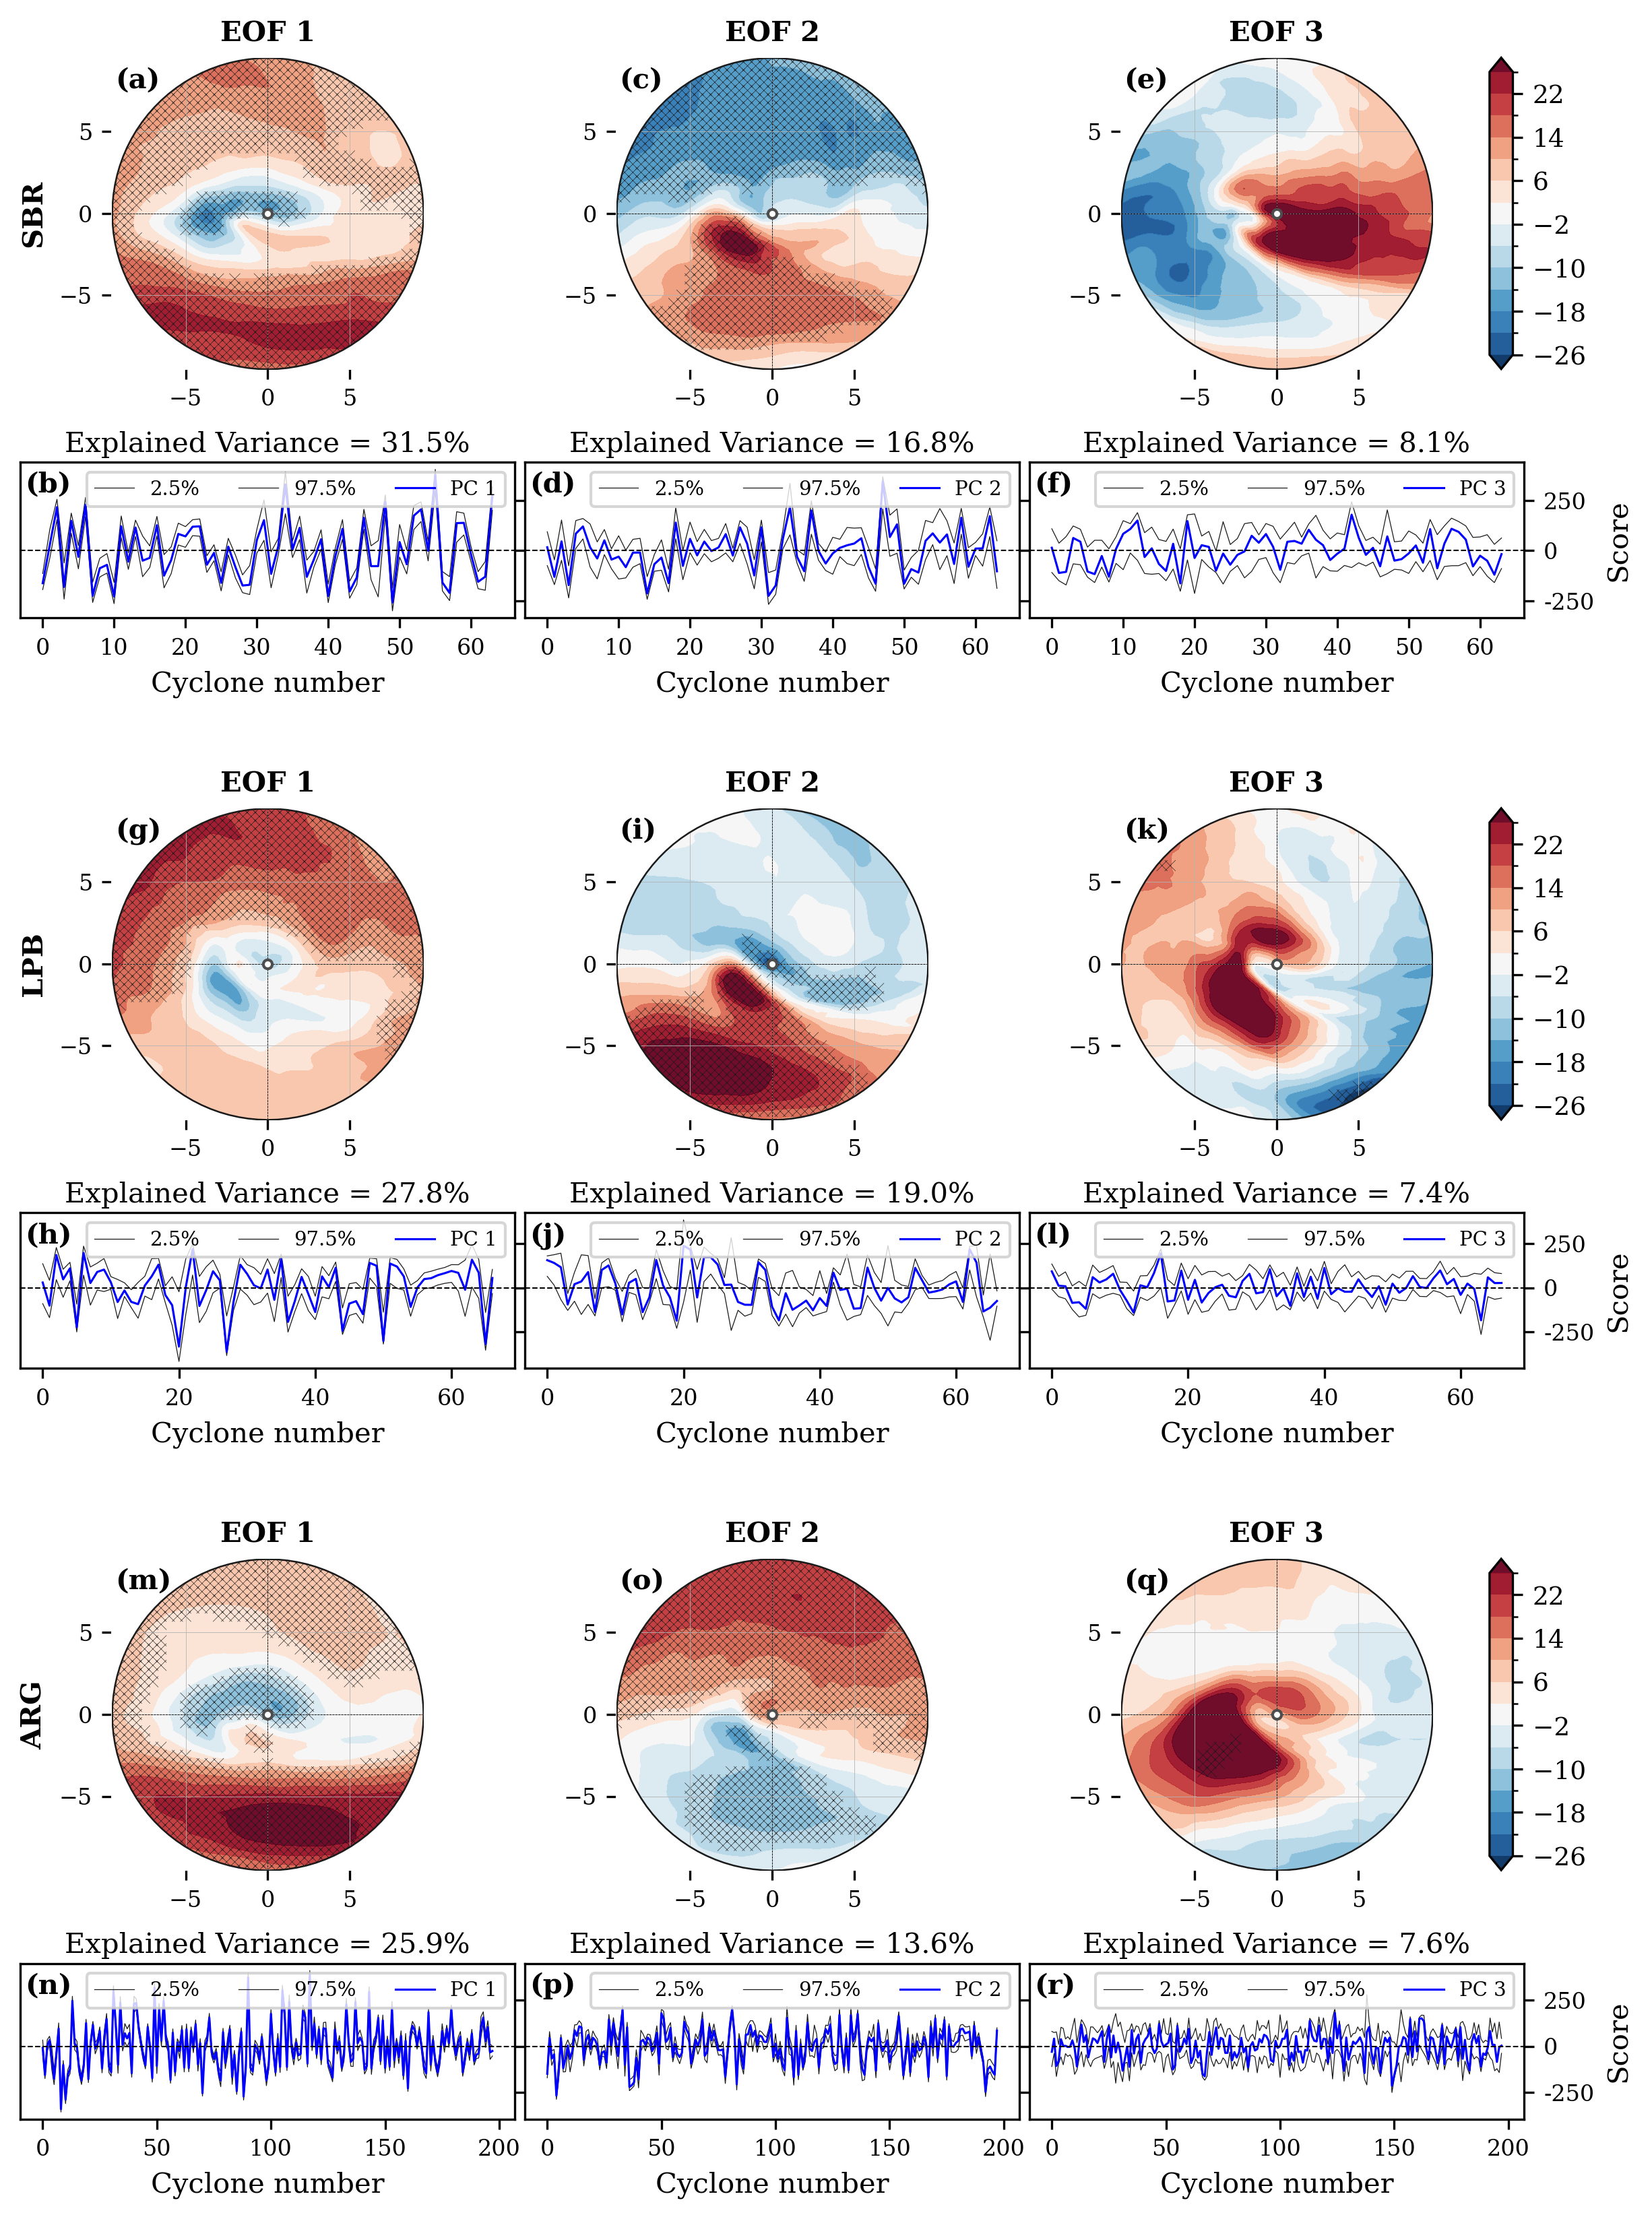
\includegraphics[width=\textwidth]{images/w10/xeof_p90_wind10_mature.png}
\caption[Significância espacial dos EOFs em fase de maturidade (subconjunto p90)]{Decomposição EOF do vento a 10~m para o subconjunto intenso (p90) em fase de maturidade. A disposição de painéis é idêntica à Figura~\ref{fig:xeof_madurez_global}.}
\label{fig:xeof_madurez_p90}
\end{figure}

Na População Global (Figura~\ref{fig:xeof_madurez_global}), EOF1 é significativo em todo o domínio nas três regiões (painéis a, g e~m).
Em concordância com sua alta variância explicada (43--57\%), as componentes PC1 (painéis b, h e~n) apresentam amplitudes maiores do que as de PC2 e PC3 nas três regiões.

EOF2 e EOF3 são significativos na maior parte de sua estrutura, e só perdem significância na transição entre seus polos, onde os valores são próximos de zero. EOF2 mostra um dipolo norte--sul nas três regiões, com valores negativos ao norte e positivos ao sul (painéis c, i e~o), e EOF3 um dipolo nordeste--sudoeste em SBR (painel~e) e leste-nordeste--oeste-sudoeste em LPB e ARG (painéis k e~q). Por construção, EOF2 representa a variância ortogonal ao modo dominante \citep{hannachi2007empirical}, e nesse campo de vento descreve uma oscilação norte--sul que abrange todo o domínio, diferentemente das estruturas compactas próximas do núcleo que o EOF2 de p90 apresenta.

As componentes PC2 e PC3 apresentam amplitudes semelhantes entre si e menores do que as de PC1 nas três regiões (painéis d, f, j, l, p e~r), em concordância com sua menor variância explicada (EOF2: 7.5--11.5\%, EOF3: 5.4--6.3\%). Como na População Global a separação entre autovalores é grande, os modos secundários descrevem uma variabilidade residual. Ainda assim, EOF2 explica mais variância em ARG (11.5\%) do que em SBR (8.7\%) e LPB (7.5\%), o que sugere processos mais complexos em ARG durante a maturidade. Já o EOF3 explica uma variância semelhante nas três regiões e tem uma estrutura parecida, o que indica que esse dipolo é uma fonte comum de variabilidade residual na maturidade.

Em p90 (Figura~\ref{fig:xeof_madurez_p90}), a significância de EOF1 se limita aos valores altos e médios do padrão e não inclui os valores próximos de zero. Em SBR (painel~a) e ARG (painel~m), tanto as anomalias positivas quanto o núcleo negativo próximo do centro são significativos, enquanto em LPB (painel~g) apenas as anomalias positivas o são, e o núcleo negativo não é significativo. Portanto, em SBR e ARG o EOF1 representa de forma robusta tanto a estrutura de maior escala quanto o núcleo localizado próximo do centro, enquanto em LPB apenas a primeira.

Diferentemente da População Global, onde EOF2 e EOF3 descrevem uma variabilidade residual, em p90 EOF2 (painéis c, i e~o) é significativo em ambos os sinais nas três regiões, exceto nos valores próximos de zero, com uma extensão comparável à de EOF1. EOF3 (painéis e, k e~q), por sua vez, praticamente não apresenta áreas significativas. EOF2 mostra estruturas compactas próximas do núcleo nas três regiões, na zona onde costuma se localizar o jato do CCB, na cauda da frente curvada (\textit{bent-back front}), onde \citet{schemm2014linkage} situam os ventos mais intensos em níveis baixos (Seção~\ref{subsec:tb_modelos}).

As componentes principais mostram o mesmo. Em p90, as amplitudes de PC2 (painéis d, j e~p) são semelhantes às de PC1 (painéis b, h e~n), enquanto as de PC3 (painéis f, l e~r) são claramente menores. Diferentemente da População Global, onde PC2 e PC3 têm amplitudes semelhantes entre si e menores do que PC1, em p90 apenas PC2 se aproxima do modo dominante, em concordância com o achatamento do espectro de autovalores (Seção~\ref{sec:var_exp_wind10}) e com o fato de que o EOF3 quase não apresenta áreas significativas.

Em conjunto, na População Global o EOF1, significativo em todo o domínio, permite descrever o campo de vento com um único modo dominante. Em p90, por sua vez, o EOF2 também é significativo e representa parte da variabilidade próxima do núcleo, onde se concentram os ventos mais intensos, o que indica que esse padrão é recorrente entre os ciclones intensos, além do mecanismo físico que se lhe atribua.

\section{Componentes principais (PC1--PC3)}\label{subsec:res_dinamica_pc1}

A distribuição da variância entre vários modos em p90 (Seção~\ref{sec:var_exp_wind10}) se reflete também nas componentes principais. Na População Global, PC1 apresenta amplitudes maiores do que as de PC2 e PC3, enquanto em p90 as amplitudes de PC2 se aproximam das de PC1 (Figura~\ref{fig:xeof_madurez_p90}). Embora PC1 mantenha uma correlação significativa com a vorticidade em todas as fases, em p90 PC2 e PC3 também apresentam correlações de magnitude comparável (Seção~\ref{subsec:pc1_p90_wind10}).

\begin{table}[htbp]
\centering
\caption[Momentos estatísticos e correlação de PC1--PC3 do vento a 10 m - População Global]
{Assimetria ($\gamma_1$) e curtose ($\gamma_2$) da PC1 do vento a 10 metros, e correlação de Spearman em valor absoluto ($|r|$) entre PC1, PC2 e PC3 e a vorticidade relativa a 850 hPa associada à fase, para a População Global. Reporta-se o valor absoluto porque o sinal da correlação depende da convenção de sinal arbitrária de cada EOF (Seção~\ref{subsec:analisis_pc}); o relevante é a magnitude da correlação e sua significância. Os valores significativos ($p<0.05$) são mostrados em negrito.}
\label{tab:stat_global_w10}
\begin{tabular*}{\textwidth}{@{\extracolsep{\fill}}llrrrrr}
\hline
\textbf{Região} & \textbf{Fase} & \textbf{Assimetria ($\gamma_1$)} & \textbf{Curtose ($\gamma_2$)} & \textbf{$|$PC1$|$} & \textbf{$|$PC2$|$} & \textbf{$|$PC3$|$} \\
\hline
\textbf{SBR} & Incipiente       & 0.58  & -0.12 & \textbf{0.57} & \textbf{0.20} & \textbf{0.37} \\
             & Intensificação & 0.26  & -0.91 & \textbf{0.80} & 0.02 & \textbf{0.32} \\
             & Maturidade         & 0.30  & -0.86 & \textbf{0.89} & 0.04 & \textbf{0.25} \\
             & Decaimento     & 0.24  & -0.79 & \textbf{0.83} & \textbf{0.12} & \textbf{0.13} \\
\hline
\textbf{LPB} & Incipiente       & 0.99  & 1.32  & \textbf{0.35} & \textbf{0.14} & \textbf{0.16} \\
             & Intensificação & 0.17  & -1.03 & \textbf{0.71} & \textbf{0.18} & \textbf{0.12} \\
             & Maturidade         & -0.09 & -1.01 & \textbf{0.87} & \textbf{0.09} & \textbf{0.19} \\
             & Decaimento     & -0.11 & -0.77 & \textbf{0.83} & \textbf{0.11} & \textbf{0.09} \\
\hline
\textbf{ARG} & Incipiente       & 0.31  & -0.13 & \textbf{0.43} & \textbf{0.24} & \textbf{0.06} \\
             & Intensificação & -0.22 & -0.37 & \textbf{0.67} & \textbf{0.11} & \textbf{0.05} \\
             & Maturidade         & -0.12 & -0.43 & \textbf{0.86} & \textbf{0.05} & \textbf{0.26} \\
             & Decaimento     & -0.06 & -0.30 & \textbf{0.76} & 0.04 & \textbf{0.28} \\
\hline
\end{tabular*}
\end{table}


\subsection{Relação com a intensidade na População Global}\label{subsec:pc1_global_wind10}

A Tabela~\ref{tab:stat_global_w10} apresenta a assimetria e a curtose de PC1, e a correlação de Spearman em valor absoluto entre PC1, PC2 e PC3 e a vorticidade relativa a 850~hPa de cada fase, para a População Global (Seção~\ref{subsec:analisis_pc}).

Na intensificação e na maturidade, a curtose de PC1 varia entre $-0.37$ e $-1.03$ nas três regiões, o que indica distribuições platicúrticas, sem caudas extremas. LPB apresenta a distribuição mais assimétrica na fase incipiente (assimetria $+0.99$, curtose $+1.32$), enquanto SBR e ARG são mais homogêneas desde as primeiras fases. A correlação de PC1 com a vorticidade aumenta em magnitude em todas as regiões desde a fase incipiente, entre $|r|=0.35$ (LPB) e $0.57$ (SBR), até um máximo na maturidade ($|r|=0.89$ em SBR, $0.87$ em LPB e $0.86$ em ARG), e diminui levemente no decaimento ($|r| > 0.75$). Isso indica que a posição de cada ciclone em relação ao padrão dominante está cada vez mais associada à sua intensidade à medida que o vórtice matura. PC2 é significativa na maioria das combinações de região e fase, com magnitudes fracas ($|r| \leq 0.24$), enquanto PC3 é significativa nas doze combinações e alcança $|r|=0.37$ (SBR incipiente) e $0.32$ (SBR intensificação), valores menores do que os de PC1. Portanto, já na População Global PC2 e PC3 não são puro ruído, embora seu peso seja sempre menor do que o de PC1.
A assimetria de PC1 tende a zero à medida que o vórtice se intensifica, o que indica que os campos de vento se organizam cada vez mais em torno do primeiro modo. Na maioria dos ciclones, o vento se organiza em torno de um padrão coerente (EOF1), enquanto em p90 esse padrão perde dominância sem desaparecer (Seção~\ref{subsec:pc1_p90_wind10}).
SBR apresenta uma correlação moderada desde a fase incipiente, enquanto em LPB a correlação aumenta de forma marcada na intensificação ($|r|$ de $0.35$ para $0.59$). Essa mudança poderia estar relacionada ao estabelecimento do forçante baroclínico nessa fase (Seção~\ref{subsec:tb_lpb}) e coincide com a fase em que a PDFe de LPB alcança sua maior densidade (Seção~\ref{sec:kde_espacial_global}).

\begin{table}[htbp]
\centering
\caption[Momentos estatísticos e correlação de PC1--PC3 do vento a 10 m - Subconjunto p90]
{Assimetria ($\gamma_1$) e curtose ($\gamma_2$) da PC1 do vento a 10 metros, e correlação de Spearman em valor absoluto ($|r|$) entre PC1, PC2 e PC3 e a vorticidade relativa a 850 hPa associada à fase, para o subconjunto extremo (p90). Reporta-se o valor absoluto porque o sinal da correlação depende da convenção de sinal arbitrária de cada EOF (Seção~\ref{subsec:analisis_pc}); o relevante é a magnitude da correlação e sua significância. Os valores significativos ($p<0.05$) são mostrados em negrito.}
\label{tab:stat_p90_w10}
\begin{tabular*}{\textwidth}{@{\extracolsep{\fill}}llrrrrr}
\hline
\textbf{Região} & \textbf{Fase} & \textbf{Assimetria ($\gamma_1$)} & \textbf{Curtose ($\gamma_2$)} & \textbf{$|$PC1$|$} & \textbf{$|$PC2$|$} & \textbf{$|$PC3$|$} \\
\hline
\textbf{SBR} & Incipiente       & 0.16  & -0.56 & \textbf{0.53} & 0.08 & \textbf{0.58} \\
             & Intensificação & -0.25 & -0.65 & \textbf{0.45} & \textbf{0.27} & \textbf{0.58} \\
             & Maturidade         & 0.36  & -0.55 & \textbf{0.44} & 0.19 & 0.12 \\
             & Decaimento     & 1.15  & 3.95  & \textbf{0.66} & \textbf{0.37} & 0.20 \\
\hline
\textbf{LPB} & Incipiente       & 0.77  & 0.42  & \textbf{0.43} & 0.08 & 0.17 \\
             & Intensificação & -0.88 & 0.96  & \textbf{0.45} & \textbf{0.38} & \textbf{0.49} \\
             & Maturidade         & -0.93 & 0.60  & \textbf{0.37} & 0.04 & 0.23 \\
             & Decaimento     & -0.20 & -0.18 & \textbf{0.54} & \textbf{0.37} & \textbf{0.56} \\
\hline
\textbf{ARG} & Incipiente       & 0.29  & -0.14 & \textbf{0.43} & \textbf{0.21} & 0.09 \\
             & Intensificação & -0.38 & -0.19 & \textbf{0.32} & \textbf{0.15} & \textbf{0.38} \\
             & Maturidade         & 0.41  & 0.25  & \textbf{0.26} & \textbf{0.32} & \textbf{0.33} \\
             & Decaimento     & 0.51  & 1.66  & \textbf{0.74} & 0.04 & \textbf{0.20} \\
\hline
\end{tabular*}
\end{table}


\subsection{Relação com a intensidade no subconjunto p90}\label{subsec:pc1_p90_wind10}

A Tabela~\ref{tab:stat_p90_w10} apresenta as mesmas estatísticas para p90. Diferentemente da precipitação (Seção~\ref{subsec:pc1_p90_tp}), a correlação entre PC1 e a vorticidade se mantém significativa em p90 nas três regiões e nas quatro fases, embora com valores de menor magnitude do que na População Global, entre $|r|=0.26$ (ARG, maturidade) e $0.74$ (ARG, decaimento). Isso indica que, mesmo nos ciclones mais intensos, a organização do vento em torno do modo dominante continua associada à intensidade do sistema.

Na intensificação, LPB apresenta uma distribuição leptocúrtica ($\gamma_2 = +0.96$) com assimetria negativa ($\gamma_1 = -0.88$), ou seja, com um pico agudo e alguns casos atípicos em direção a valores baixos. SBR mantém distribuições estáveis durante o desenvolvimento, mas no decaimento apresenta uma curtose muito alta ($\gamma_2 = +3.95$) e assimetria positiva ($+1.15$), o que sugere que os ciclones intensos não seguem um único caminho até a dissipação.

O traço distintivo de p90 não é a perda de correlação de PC1 com a vorticidade, mas sim que PC2 e PC3 apresentam correlações de maior magnitude do que na População Global (Seção~\ref{subsec:pc1_global_wind10}), embora significativas em menos combinações. PC3 supera até mesmo PC1 em SBR durante a fase incipiente ($|r|=0.58$ contra $0.53$) e a intensificação ($0.58$ contra $0.45$), e em LPB durante a intensificação ($0.49$ contra $0.45$) e o decaimento ($0.56$ contra $0.54$). Em ARG, PC2 e PC3 são significativas junto com PC1 durante a maturidade ($|r|=0.32$ e $0.33$, respectivamente), e no decaimento apenas PC3 ($|r|=0.20$). Isso concorda com a distribuição da variância entre vários modos em p90 (Seção~\ref{sec:var_exp_wind10}) e indica que os modos secundários também estão associados à intensidade do vórtice.

Consequentemente, nos ciclones mais intensos a PC1 não resume por si só a organização do vento, já que os modos secundários, que poderiam representar estruturas de mesoescala, também estão associados à intensidade, e descrever o vento desses ciclones apenas com o modo dominante resultaria incompleto. Essa limitação se relaciona com o apontado por \citet{sinclair1997objective}, que mostra que a circulação, ao integrar o tamanho e a rotação do sistema, é uma medida mais representativa da intensidade de um ciclone do que a vorticidade local.

\section{Síntese}\label{sec:sintesis_wind10}

A análise do vento a 10~m mostra que os ciclones intensos não são uma versão amplificada da população média, mas diferem na magnitude, na localização e na organização espacial de seus ventos máximos.

\paragraph{Magnitude.}
Na População Global, a moda dos máximos de vento se situa entre 11 e 14~m\,s$^{-1}$ na fase incipiente e entre 16 e 19~m\,s$^{-1}$ na maturidade. Em p90, a moda da maturidade se desloca para 23--25~m\,s$^{-1}$, entre 25\% e 50\% acima da População Global, com caudas de até 30~m\,s$^{-1}$, valores coerentes com os reportados para ciclones do Atlântico Sul. Os picos de p90 são semelhantes entre regiões, embora ARG estenda mais sua cauda em direção a velocidades altas.

\paragraph{Localização.}
Na População Global, os máximos se distribuem de forma difusa e se deslocam do setor leste nas primeiras fases ao quadrante noroeste na maturidade. Em p90, esse deslocamento é mais marcado, e na maturidade os máximos se concentram fortemente no quadrante noroeste, a ${\sim}$2--4$^{\circ}$ do centro, na zona onde a literatura situa o jato da cinta transportadora fria (CCB) e a fratura frontal. Essa concentração é maior em SBR e LPB do que em ARG, embora SBR apresente a distribuição de magnitudes mais larga das três regiões, o que indica que concentrar a localização dos máximos não implica concentrar sua magnitude. No decaimento, o núcleo de p90 permanece no noroeste, enquanto na População Global a densidade diminui e sua localização varia entre regiões.

\paragraph{Padrões de variabilidade.}
Na População Global, EOF1 explica entre 30.9\% e 57.4\% da variância, forma um gradiente norte--sul de grande escala e é significativo em todo o domínio, de modo que um único modo descreve grande parte da variabilidade do vento. Em p90, EOF1 não supera 37.6\% e a variância se distribui entre vários modos. Na maturidade, EOF1 apresenta um núcleo negativo compacto próximo do centro, significativo em SBR e ARG mas não em LPB, e EOF2 é significativo com uma extensão comparável à de EOF1 e estruturas compactas próximas do núcleo, enquanto EOF3 quase não apresenta áreas significativas. Essa organização é compatível com um maior peso da variabilidade de mesoescala nos ciclones intensos.

\paragraph{Relação com a intensidade.}
Na População Global, a correlação entre PC1 e a vorticidade aumenta até valores de $|r|=0.86$ a $0.89$ na maturidade. Em p90, mantém-se significativa em todas as regiões e fases, embora com valores de menor magnitude (entre $|r|=0.26$ e $0.74$), diferentemente do que ocorre com a precipitação (Capítulo~\ref{cap:resultados_tp}). Ao mesmo tempo, PC2 e PC3 apresentam em p90 correlações de maior magnitude do que na População Global, e em quatro combinações de região e fase superam as de PC1. Nos ciclones intensos, o modo dominante não resume por si só a relação entre a organização do vento e a intensidade do sistema.

\paragraph{Alcance.}
Esses resultados dependem da vorticidade de cada fase como medida pontual de intensidade e poderiam diferir com uma medida integrada de circulação \citep{sinclair1997objective}. Além disso, o ERA5 tende a subestimar as magnitudes extremas (Seção~\ref{sec:datos_era5}), e a relação do núcleo noroeste com o \textit{sting jet} e o CCB se apoia principalmente em estudos do Hemisfério Norte e na simetria entre hemisférios, já que a climatologia global desses sistemas não distingue o Atlântico Sul \citep{gray2024global}.

O Capítulo~\ref{cap:resultados_tp} aplica a mesma análise à precipitação, e o Capítulo~\ref{chap:meof} avalia se os máximos de ambas as variáveis coincidem no espaço segundo a fase e a região de gênese (Seção~\ref{sec:tb_compound_def}).
		% trabalho.
\chapter{Precipitação total}\label{cap:resultados_tp}
A precipitação associada a ciclones extratropicais complementa o vento (Capítulo~\ref{cap:resultados_wind10}) na caracterização estrutural do sistema. Diferentemente do vento, ela integra processos de calor, desde a condensação estratiforme de grande escala até a convecção embutida de mesoescala ligada à liberação de calor latente (Seção~\ref{subsec:tb_modelos}).
Este capítulo estabelece a estrutura espacial da precipitação durante as fases do ciclo de vida dos ciclones extratropicais do Atlântico Sul-Ocidental, seguindo a progressão metodológica do Capítulo~\ref{cap:resultados_wind10}: (i)~evolução das distribuições de magnitude segundo a intensidade do vórtice e a região de gênese; (ii)~localização espacial preferencial dos máximos de precipitação; e (iii)~decomposição EOF.
A Seção~\ref{sec:pdf_tp} examina as PDF de magnitude; as Seções~\ref{subsec:kde_tp_global} e~\ref{subsec:kde_tp_p90}, a distribuição espacial dos máximos (PDFe); e as Seções~\ref{subsec:var_exp_tp}--\ref{sec:dinamica_pc1_tp}, a estrutura modal via EOF.
Os resultados são contrastados com os do campo de vento para avaliar, no Capítulo~\ref{chap:meof}, se ambas as variáveis compartilham uma organização espacial coerente.

% --- SEÇÃO PRINCIPAL: PDF DE PRECIPITAÇÃO TOTAL ---

\section{Distribuição de magnitudes (PDF)}\label{sec:pdf_tp}

\begin{figure}[htbp]
\centering
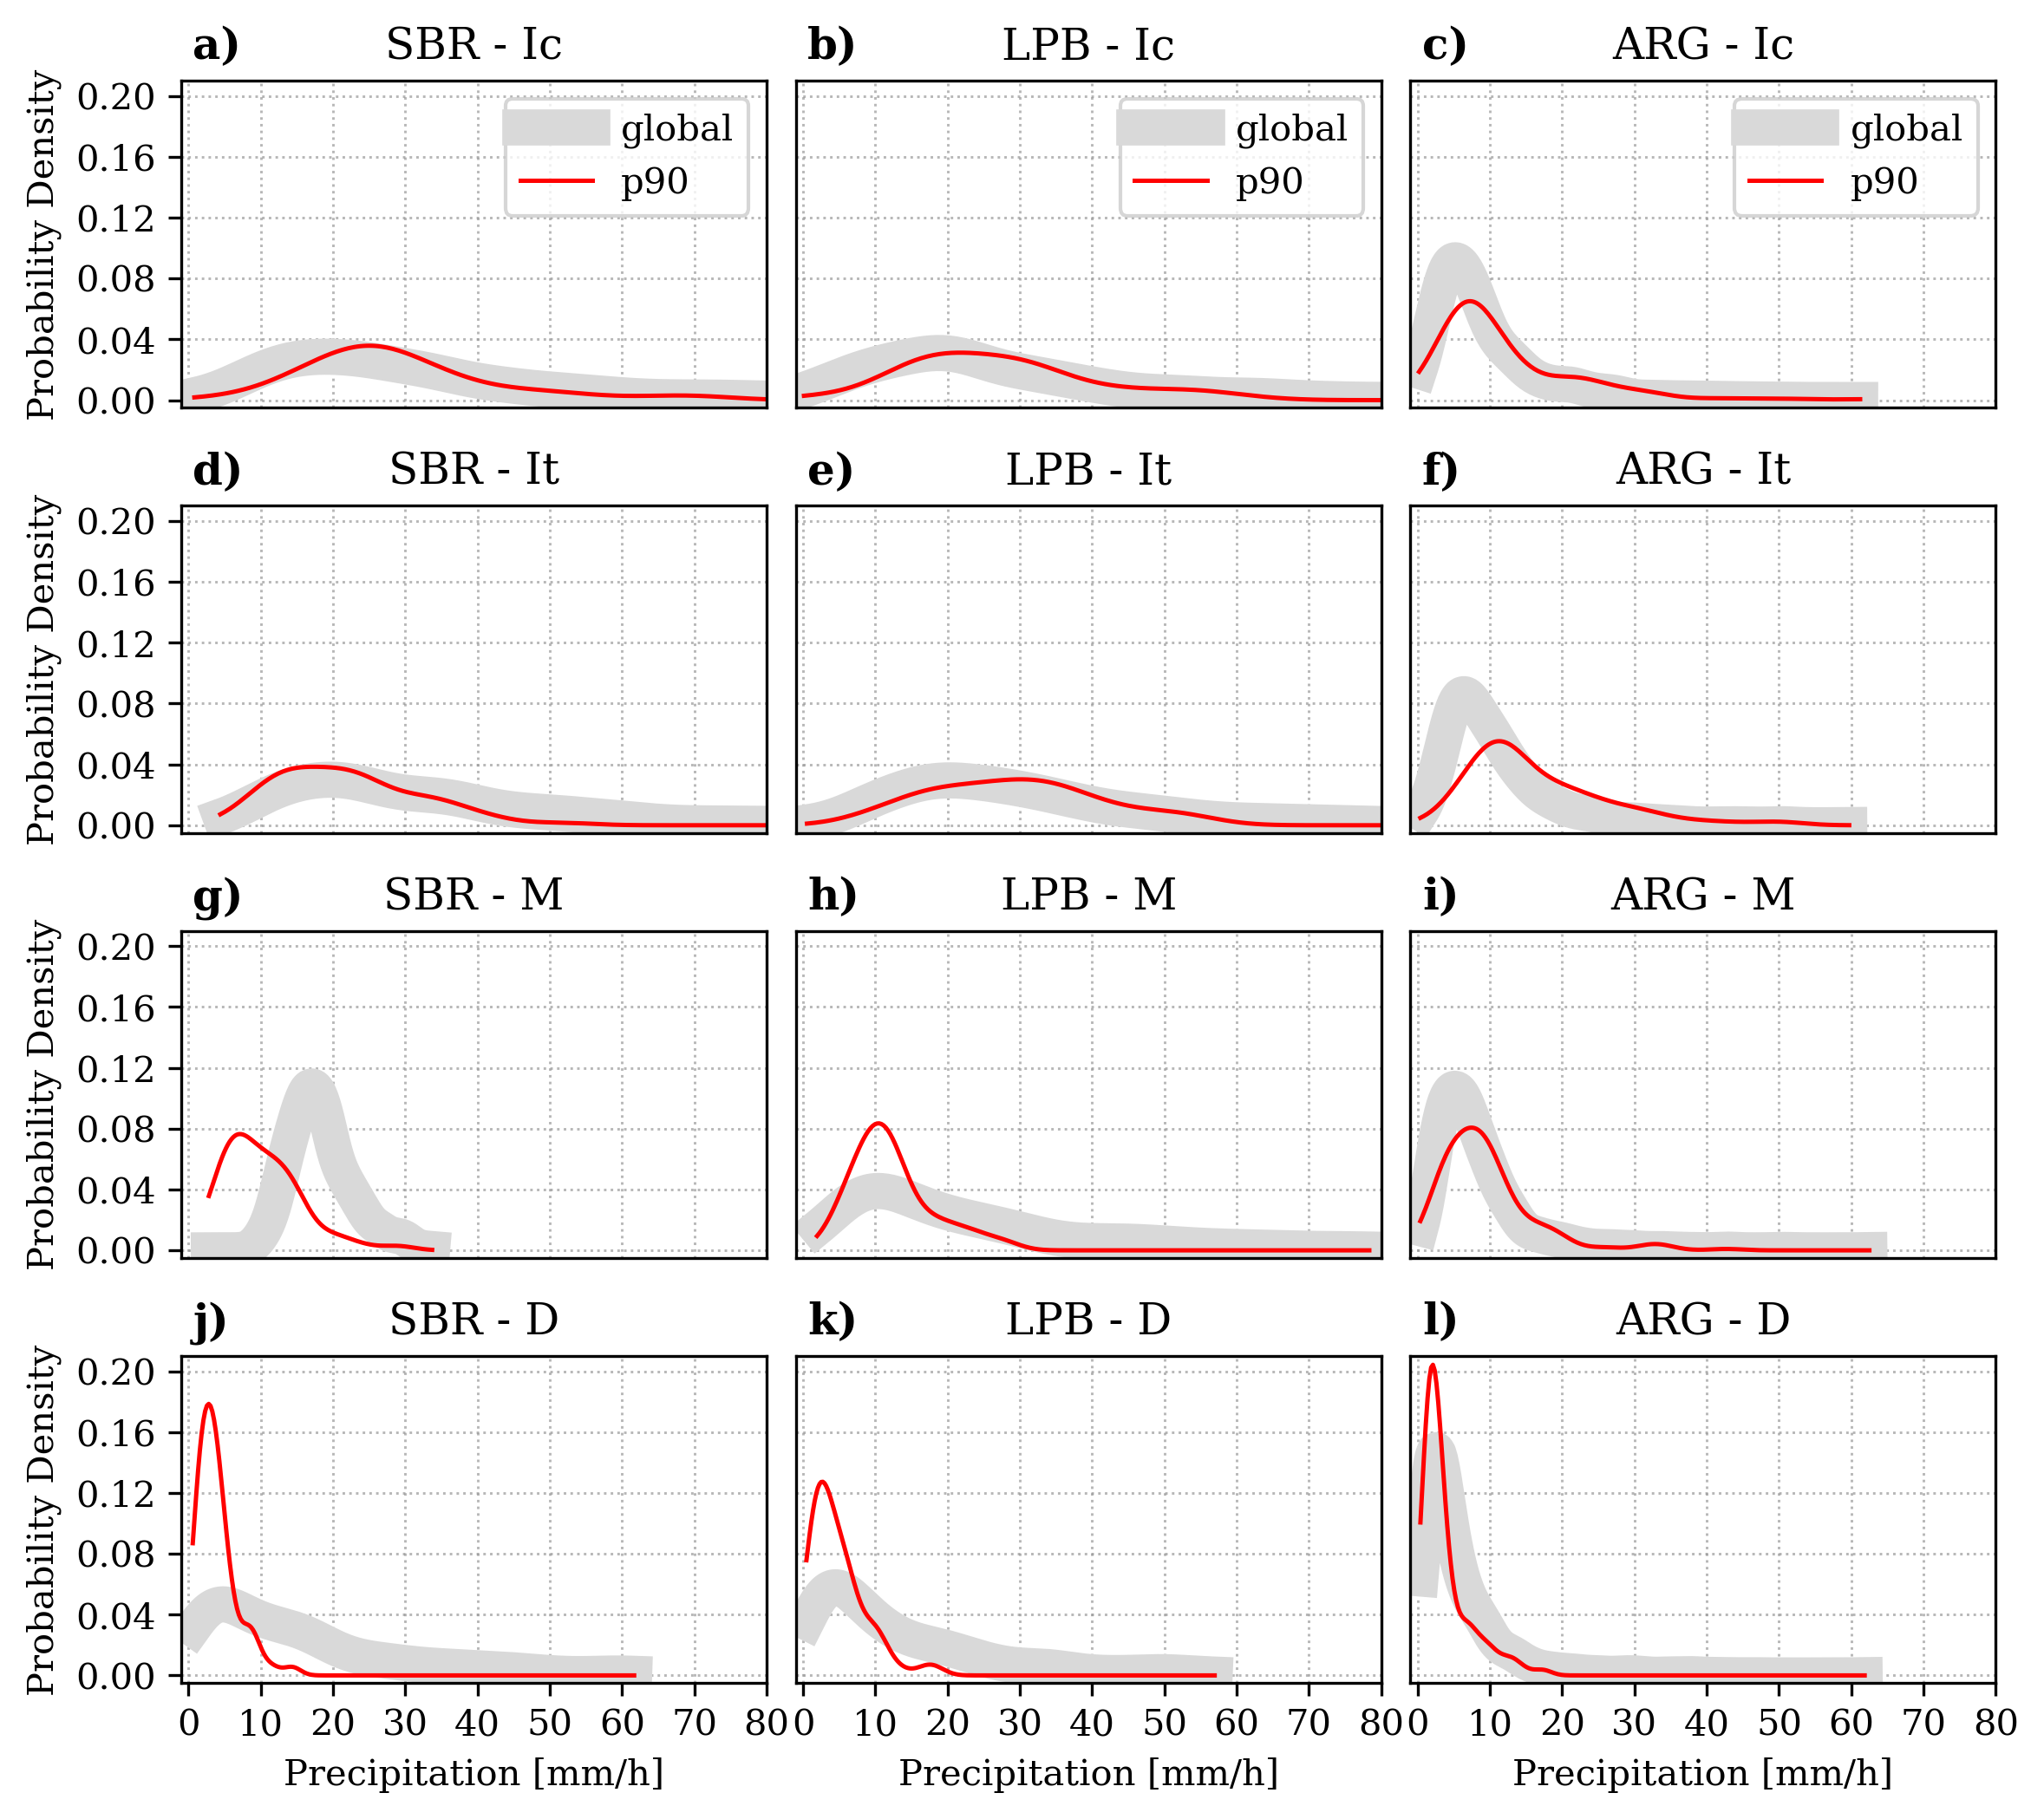
\includegraphics[width=\textwidth]{images/tp/PDF_tp_sigma025.png}
\caption[PDF de magnitudes máximas de precipitação total]{Funções de densidade de probabilidade (PDF) para as magnitudes máximas de precipitação total (mm/h). As colunas indicam a região de ciclogênese (SBR, LPB, ARG) e as linhas a evolução através das fases do ciclo de vida (Ic, It, M, D). Contrasta-se a População Global (referência, sombreado cinza) com o subconjunto dos máximos de vorticidade relativa em 850 hPa alcançados em seu ciclo de vida: p90 (ciclones intensos, linha vermelha).}
\label{fig:pdf_tp}
\end{figure}

A Figura~\ref{fig:pdf_tp} mostra a distribuição estatística dos máximos espaciais de precipitação (mm/h) para os compostos do instante central de cada fase, estratificados por região de ciclogênese (SBR, LPB, ARG) e pelo pico de vorticidade relativa em 850 hPa alcançado no ciclo de vida (p90).
Os ciclones extratropicais são a principal causa de precipitação em latitudes médias, e em simulações idealizadas os ciclones com maior vorticidade máxima produzem mais precipitação, embora essa relação seja fraca nos ciclones de latitudes altas com pouca umidade \citep{sinclair2023relationship}. A comparação entre a População Global e p90 permite avaliar se essa relação se cumpre nas regiões de estudo.
Esses campos foram extraídos dentro do domínio centrado no núcleo de cada sistema, seguindo a metodologia aplicada ao vento (Capítulo~\ref{cap:resultados_wind10}).

Nas fases incipiente e intensificação (painéis a, b, d e e), SBR e LPB mostram na População Global um perfil plano e estendido com pico modal próximo de 20~mm/h, reflexo da ampla dispersão de intensidades nessas regiões.
Em SBR e LPB, a distribuição de p90 é parecida com a da População Global da qual faz parte, embora seu pico se desloque para valores um pouco maiores em SBR durante a fase incipiente (${\sim}$25~mm/h) e em LPB durante a intensificação (${\sim}$30~mm/h). As taxas superiores a 60~mm/h aparecem com densidades muito baixas e não são mais frequentes em p90 do que na População Global, portanto não são exclusivas dos ciclones mais intensos.
No ERA5, a precipitação total é a soma da componente de grande escala e da convectiva parametrizada, e nos ciclones mais intensos é subestimada em torno de 23\% \citep{chen2024evaluation}, o que deve ser levado em conta ao interpretar os valores absolutos (Seção~\ref{sec:datos_era5}). Em ciclones do Mediterrâneo, \citet{flaounas2018heavy} encontram que as taxas mais altas (mais de 50~mm em 3~h) se devem com maior probabilidade à convecção profunda do que à Cinta Transportadora Quente (WCB, \textit{warm conveyor belt}), embora uma parte importante dessa convecção esteja embutida no WCB. Nesses ciclones, a chuva convectiva ocorre perto do centro e em seu lado leste, e a do WCB em direção ao nordeste, o que no Hemisfério Sul corresponderia ao sudeste.

Em ARG (painéis c e f), a População Global apresenta um pico pronunciado em valores baixos (${\sim}$5--6~mm/h, densidade ${\sim}$0.10) e uma queda rápida em direção a valores maiores, compatível com a menor disponibilidade de umidade em latitudes mais altas \citep{sinclair2023relationship}.
Em p90, o pico da fase incipiente se mantém em valores semelhantes, com menor densidade, enquanto na intensificação (painel f) se desloca para ${\sim}$11~mm/h, com mais casos entre 15 e 35~mm/h do que na População Global. É a separação mais clara entre p90 e a População Global nas fases iniciais, embora seus valores permaneçam muito abaixo dos de SBR e LPB.

Ao alcançar a maturidade (painéis g--i) e o decaimento (painéis j--l), as diferenças entre a População Global e p90 aumentam.
Na maturidade, a População Global de SBR apresenta um pico estreito próximo de 17~mm/h, enquanto p90 se desloca para ${\sim}$7~mm/h. Em LPB ambas têm seu pico próximo de 10~mm/h, mas a curva de p90 é mais aguda. No decaimento, a População Global de ambas as regiões se desloca para ${\sim}$5~mm/h e p90 se concentra em valores mínimos (1--4~mm/h), com densidades de ${\sim}$0.18 em SBR e ${\sim}$0.13 em LPB.
Em ARG, o decaimento (painel l) apresenta a distribuição mais concentrada da figura. O pico de p90 se localiza próximo de 2~mm/h, com uma densidade de ${\sim}$0.20, superior à de SBR e LPB, e a densidade de ambas as curvas tende a zero acima de ${\sim}$20~mm/h. Nessa fase, os ciclones de ARG produzem quase exclusivamente precipitação de baixa intensidade.

Em contraste, ARG apresenta precipitações menores em todas as fases. Isso concorda com \citet{gramcianinov2019properties}, que, a partir da precipitação média em um raio de 6° ao redor do centro, encontram que os ciclones de SBR e LPB produzem a precipitação mais intensa, com distribuições semelhantes entre ambas as regiões, enquanto em ARG são menos os ciclones que superam os 20~mm/dia. Essa diferença é coerente com o maior peso dos processos úmidos em SBR e LPB e da baroclinicidade de grande escala em ARG (Seções~\ref{subsec:tb_sbr}, \ref{subsec:tb_lpb} e~\ref{subsec:tb_arg}).

Em p90, a precipitação diminui na maturidade, fase que contém o instante de máxima intensidade para a maioria dos ciclones (Tabela~\ref{tab:fase_max_intensidad}). Essa defasagem coincide com \citet{dacre2023climatology}, que, para os 400 ciclones mais intensos segundo a vorticidade a 850~hPa nos oceanos ao redor da Austrália (maio a setembro, 1979--2021), encontram que o máximo de precipitação ocorre em média 24~h antes da intensidade máxima. Os autores explicam isso pela menor disponibilidade de umidade à medida que o ciclone se desloca em direção ao polo, ou pelo aquecimento diabático da fase de máxima precipitação, que reforça a intensidade do ciclone. Em ${\sim}$5000 ciclones invernais do Atlântico Norte, \citet{heitmann2024lifecycle} encontram que a taxa e o volume de precipitação do WCB alcançam seu máximo enquanto o ciclone ainda está se aprofundando, antes de alcançar sua pressão mínima.
Também coincide com \citet{mcerlich2023extremes}, que, em compostos de ciclones de latitudes médias do Hemisfério Sul com ERA5, encontram que a precipitação extrema ocorre com mais frequência durante o aprofundamento, antes do pico de intensidade, e que na fase de decaimento sua frequência e sua contribuição à precipitação total caem para 46\% e 80\% do valor do aprofundamento, respectivamente. Os mesmos autores encontram que a precipitação extrema se concentra em uma região menor ao redor do centro do que a precipitação não extrema.

Essa diminuição também poderia estar relacionada à chegada de ar subsidente e seco perto do centro. Em um ciclone do Hemisfério Norte com seclusão quente, \citet{shapiro1999bridge} documentam subsidência a oeste do centro e precipitação deslocada para leste, adiante da frente fria. A localização dos máximos de precipitação em relação ao centro é analisada na Seção~\ref{sec:pdfe_tp}.

% --- SEÇÃO PRINCIPAL: PDFe ESPACIAL DE PRECIPITAÇÃO ---

\section{Distribuição espacial de máximos (PDFe)}\label{sec:pdfe_tp}

\subsection{População Global}\label{subsec:kde_tp_global}

\begin{figure}[htbp]
\centering
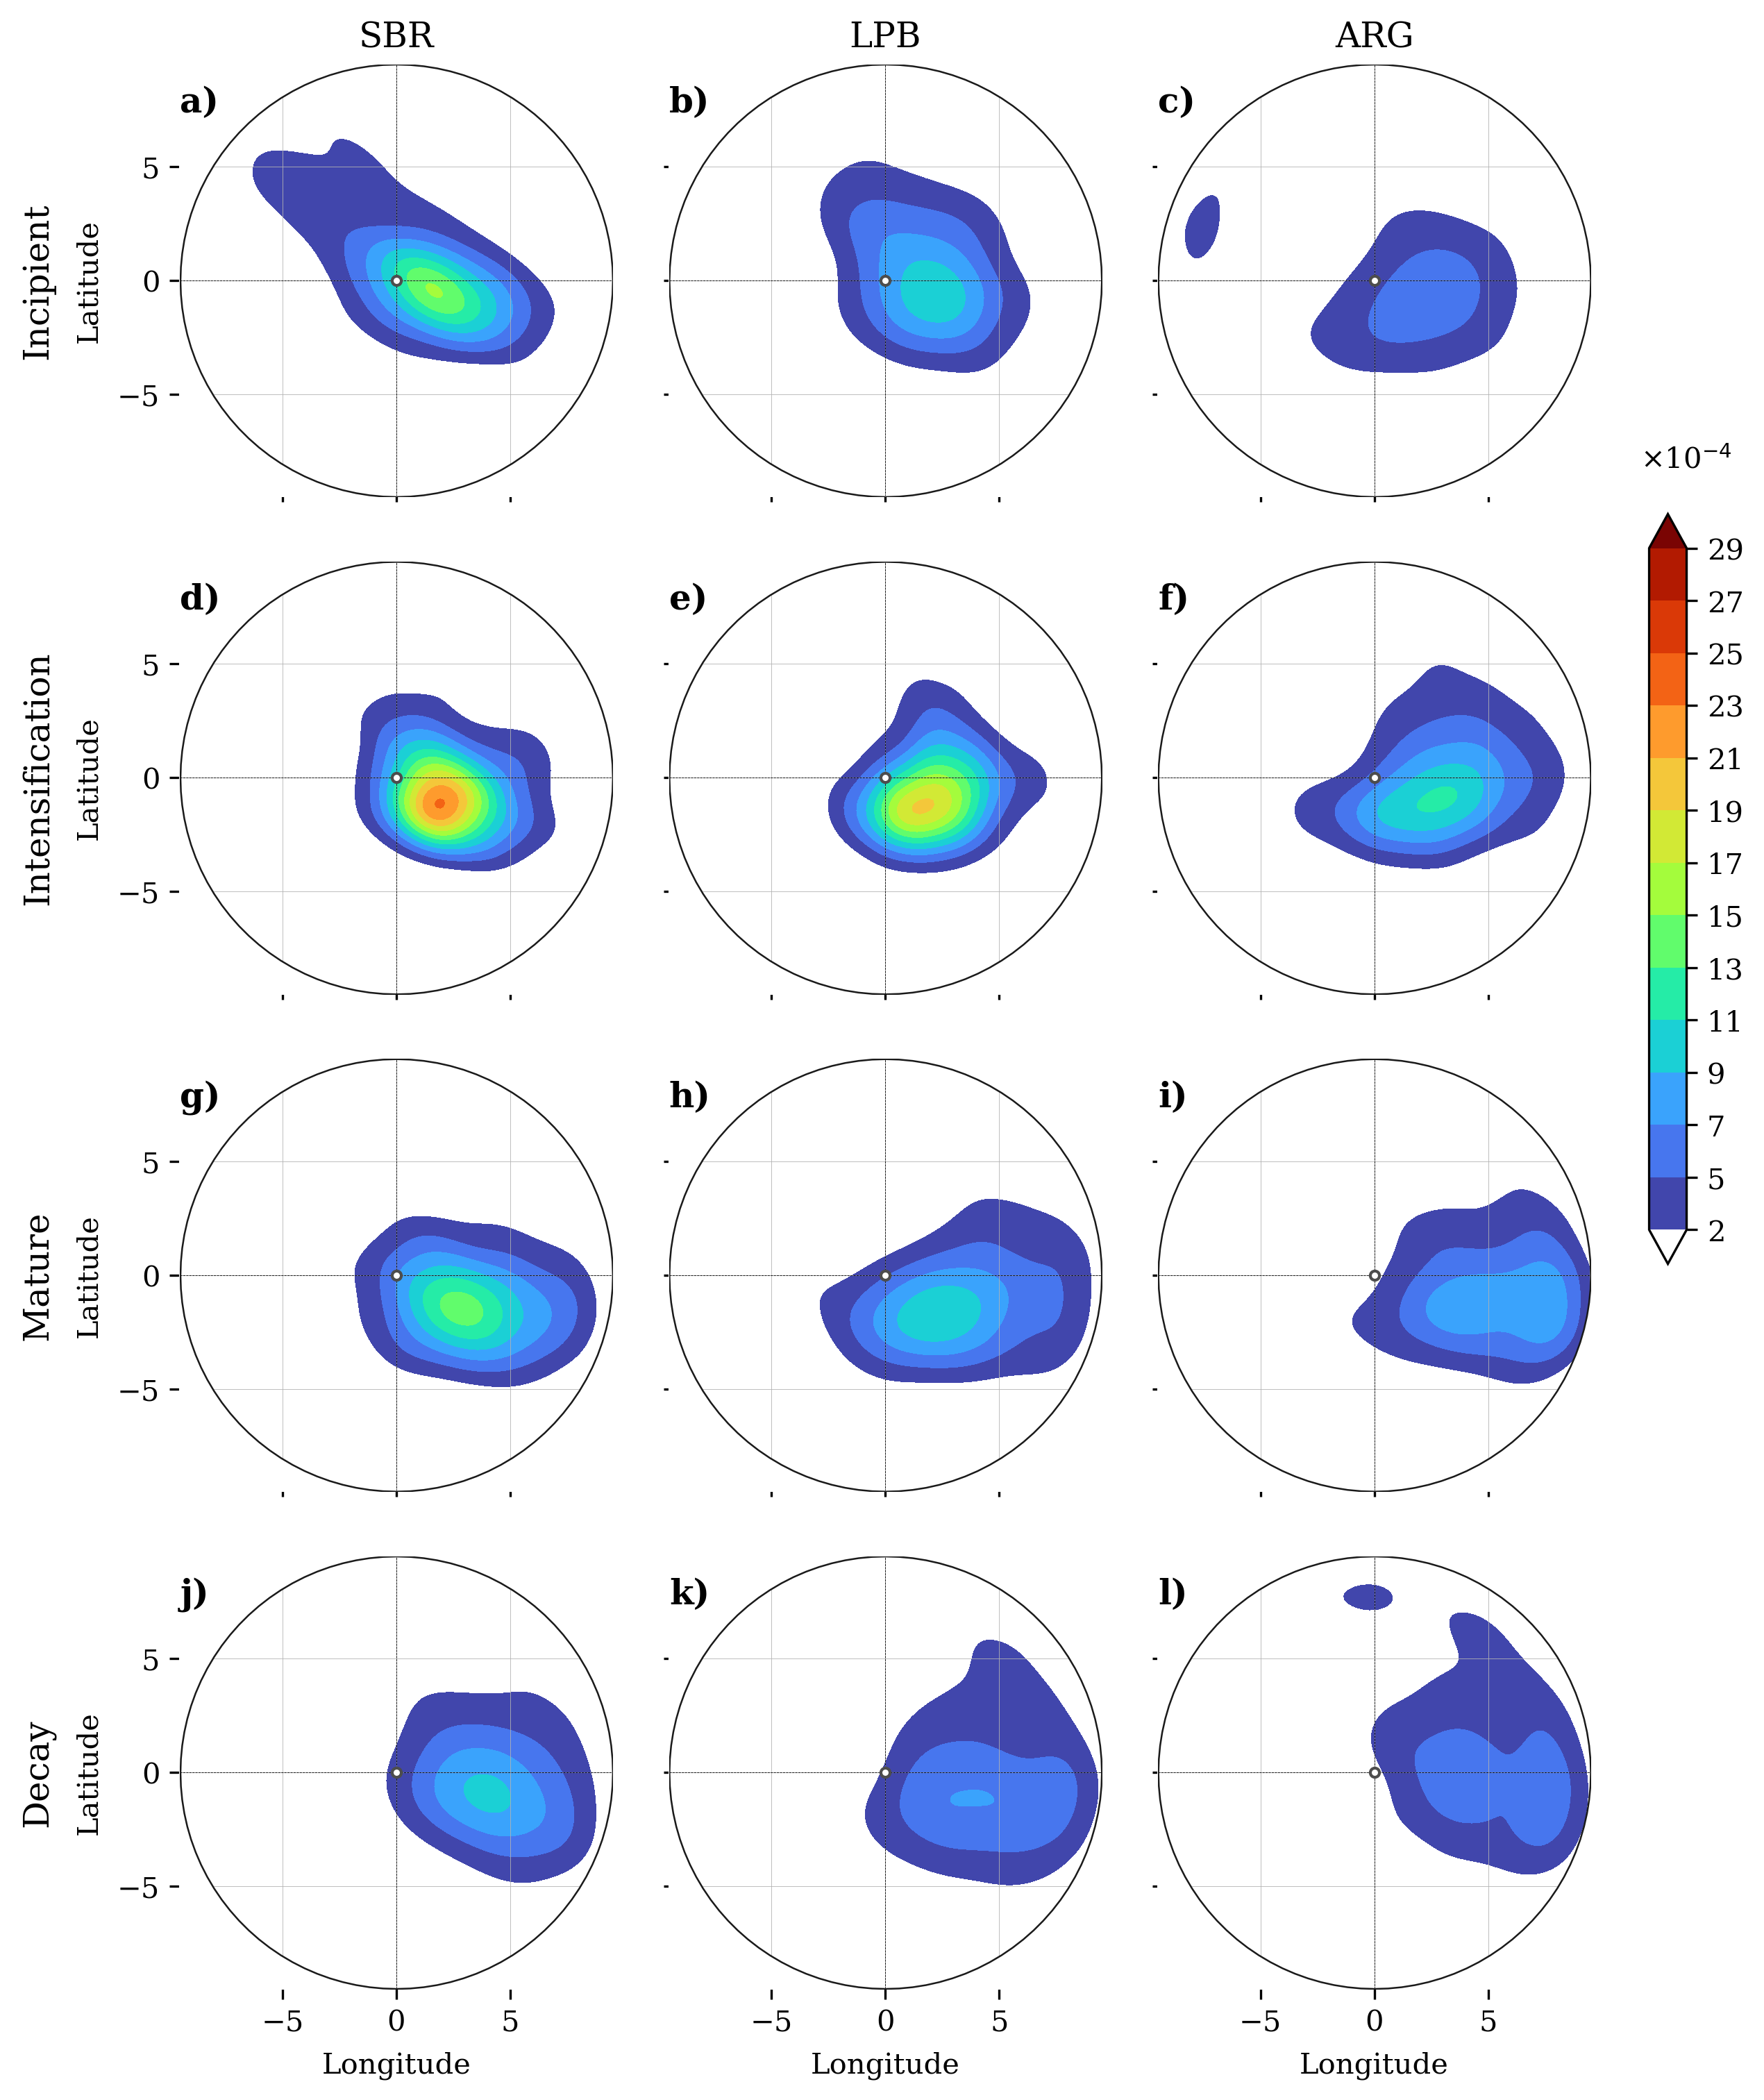
\includegraphics[width=\textwidth]{images/tp/kde_tp_global_fasesxreg.png}
\caption[PDF espacial de precipitação máxima (População Global)]{Estimação de densidade espacial bidimensional (usando estimação de densidade por kernel KDE) para a localização geométrica dos máximos de precipitação total (mm/h) na População Global de referência. A matriz organiza a evolução espacial através das fases evolutivas Incipiente (a-c), Intensificação (d-f), Maturidade (g-i) e Decaimento (j-l), segregadas pelas regiões de ciclogênese SBR, LPB e ARG. O domínio abrange $20^{\circ} \times 20^{\circ}$ com centro no vórtice $(0,0)$. A barra de cores quantifica a densidade de probabilidade relativa escalada por $10^{-4}$.}
\label{fig:kde_tp_global}
\end{figure}

A Figura~\ref{fig:kde_tp_global} mostra a densidade espacial da localização dos máximos de precipitação para a População Global.
Como no vento (Seção~\ref{sec:kde_espacial_global}), na fase incipiente os máximos se localizam a leste do centro, embora a precipitação apresente uma assimetria mais pronunciada.

Em SBR (painel a), a densidade máxima (${\approx}$\,15--17\,$\times10^{-4}$) se localiza a ${\sim}$2° a leste do centro, quase na sua mesma latitude, com uma cauda em direção ao noroeste, que é a assimetria mais notável dessa fase. LPB (painel b) apresenta um núcleo em posição similar e de menor densidade (${\approx}$\,9--11\,$\times10^{-4}$), com elongação ao norte. Em ARG (painel c), o núcleo principal se localiza a leste-sudeste (${\approx}$\,5--7\,$\times10^{-4}$) e coexiste com um foco secundário pequeno e fraco no noroeste.

A intensificação concentra as maiores densidades. Em SBR (painel d), o núcleo alcança ${\approx}$\,23--25\,$\times10^{-4}$, o máximo da figura, e se localiza a ${\sim}$2° a leste e ${\sim}$1° ao sul do centro, com contornos internos quase circulares. LPB (painel e) apresenta um núcleo na mesma posição (${\approx}$\,19--21\,$\times10^{-4}$), com a envoltória estendida em direção ao nordeste. ARG (painel f) tem a menor densidade dessa fase (${\approx}$\,11--13\,$\times10^{-4}$), com o núcleo a leste-sudeste, uma extensão em direção ao nordeste e sem o foco secundário da fase incipiente.

ARG apresenta a menor densidade da linha nas quatro fases (painéis c, f, i e l), o que é coerente com a menor precipitação dessa região descrita na Seção~\ref{sec:pdf_tp}.

Ao alcançar a maturidade, as densidades diminuem e os padrões se alargam. Em SBR (painel g), o núcleo (${\approx}$\,13--15\,$\times10^{-4}$) se localiza a ${\sim}$3° a leste e ${\sim}$1.5° ao sul do centro, com forma ovalada de eixo oeste-noroeste a leste-sudeste. LPB (painel h) apresenta um núcleo em posição semelhante (${\approx}$\,9--11\,$\times10^{-4}$), com contornos que se estendem em direção ao leste e ao nordeste. ARG (painel i) tem a menor densidade (${\approx}$\,7--9\,$\times10^{-4}$) e o núcleo mais afastado em direção ao leste da linha (${\sim}$6°). Diferentemente do vento, cujos máximos se deslocam nessa fase para o quadrante noroeste (Seção~\ref{sec:kde_espacial_global}), os máximos de precipitação permanecem a leste e sudeste do centro.

No decaimento, as densidades são baixas e os máximos se localizam mais distantes do centro, a ${\sim}$4--6° a leste, sem densidade apreciável a oeste do centro em nenhuma região. SBR (painel j) registra sua menor densidade (${\approx}$\,9--11\,$\times10^{-4}$), com os contornos restritos à metade oriental do domínio. LPB (painel k) apresenta um núcleo pequeno a leste-sudeste (${\approx}$\,7--9\,$\times10^{-4}$), com contornos que se estendem em direção ao nordeste. Em ARG (painel l), o núcleo se localiza a leste (${\approx}$\,5--7\,$\times10^{-4}$, junto com a fase incipiente a menor densidade da figura), com um foco isolado e fraco no extremo norte do domínio.

A localização dos máximos a leste e sudeste do centro na População Global coincide com a que a literatura atribui à precipitação do WCB. No modelo conceitual de \citet{browning1986conceptual}, o WCB ascende adiante da frente fria e sobre a frente quente, no setor quente do ciclone. Em compostos de precipitação média de ciclones oceânicos de ambos os hemisférios, \citet{naud2020evaluation} situam o máximo a ${\sim}$250~km do centro, em direção ao polo e a leste, e um mínimo a oeste, o que no Hemisfério Sul corresponde ao sudeste. Em SBR e LPB, os núcleos das fases incipiente e intensificação se localizam a uma distância semelhante (${\sim}$2° a leste e 0.5--1.3° ao sul), e a oeste do centro a densidade é baixa, exceto a cauda noroeste da fase incipiente.
Em escala global, \citet{catto2015fronts} encontram que, em partes das latitudes médias, mais de 60\% dos eventos de precipitação extrema coincidem com frentes, até 90\% deles associados a um WCB, e que as frentes com WCB têm entre 2 e 10 vezes mais probabilidade de produzir precipitação extrema do que as frentes sem WCB.

As maiores densidades de SBR e LPB poderiam estar relacionadas ao transporte de umidade desde latitudes tropicais ao longo do flanco oriental do ciclone em níveis baixos, que \citet{vera2002cold} documentam para as ondas sinóticas da estação fria sobre a América do Sul subtropical e que favorece a precipitação no sudeste do continente.

Na maturidade e no decaimento (painéis g--l), os máximos permanecem a leste do centro, mas se afastam dele e se dispersam. Como a População Global inclui os ciclones p90, a seção seguinte examina se os ciclones mais intensos se afastam desse padrão.

\subsection{Subconjunto de ciclones intensos p90}\label{subsec:kde_tp_p90}

\begin{figure}[htbp]
\centering
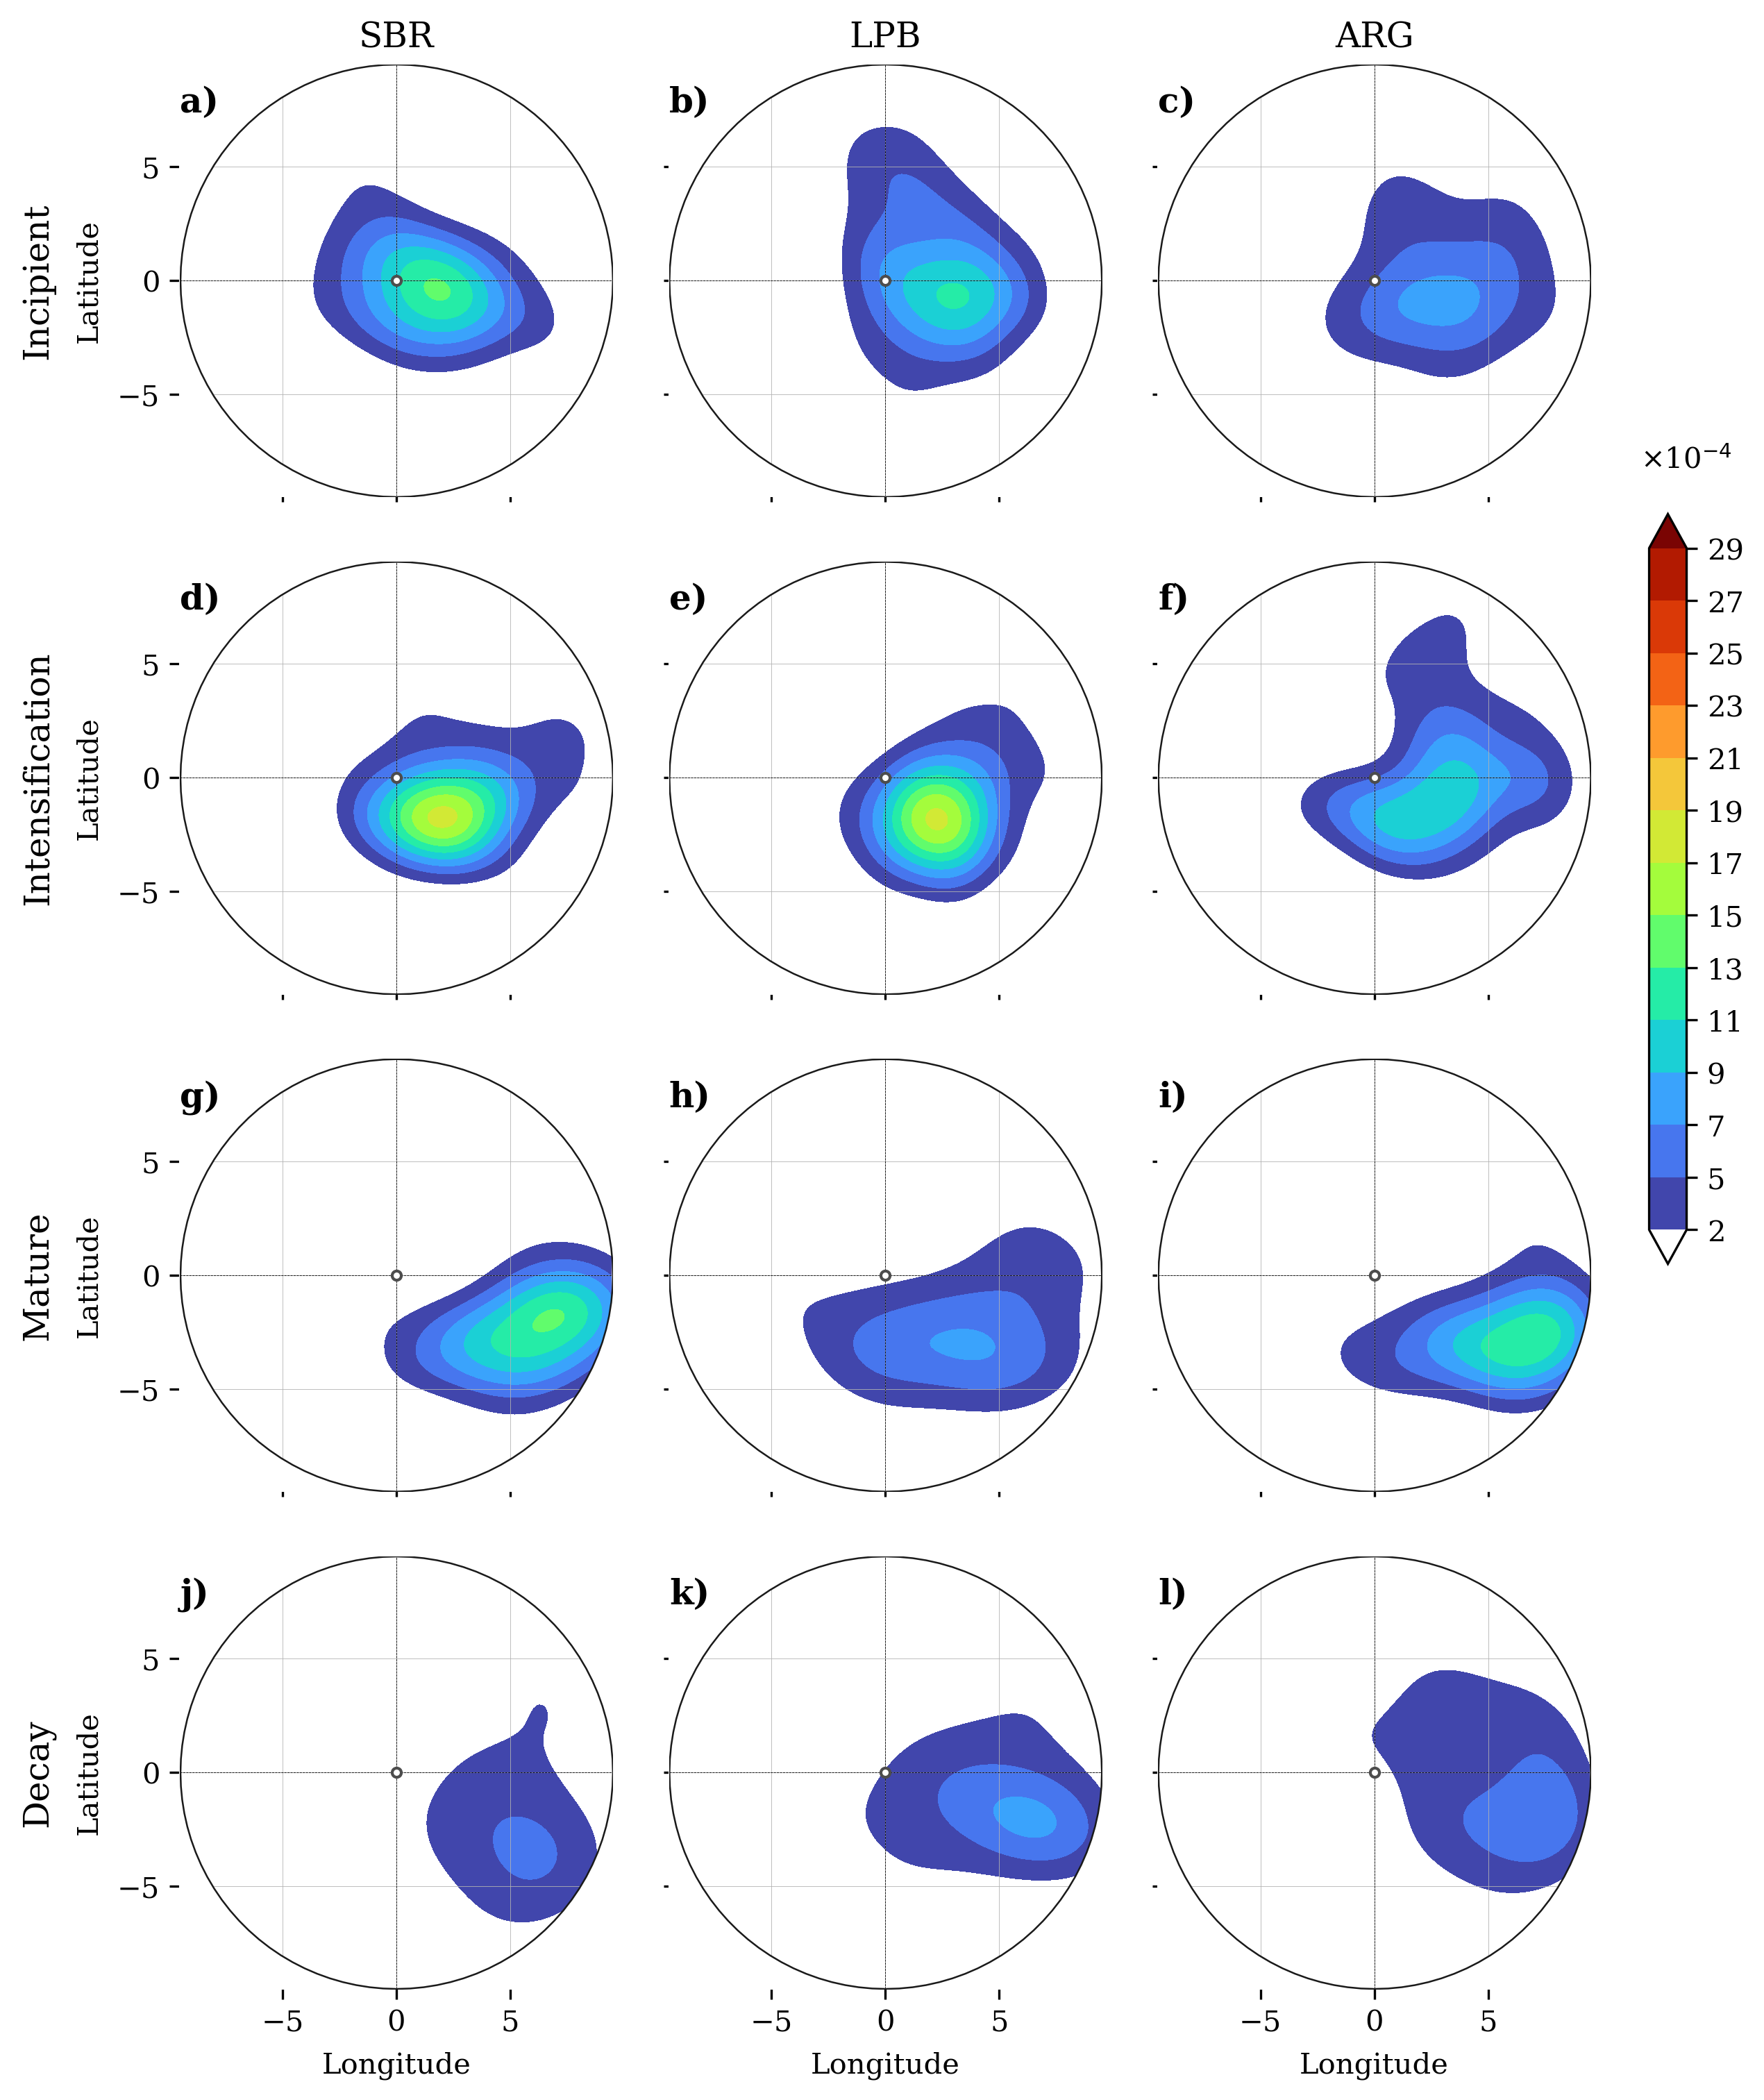
\includegraphics[width=\textwidth]{images/tp/kde_tp_p90_fasesxreg.png}
\caption[PDF espacial de precipitação máxima (subconjunto p90)]{Estimação de densidade espacial bidimensional (PDFe) para a localização geométrica dos máximos de precipitação total (mm/h) correspondente ao subconjunto de ciclones intensos (percentil 90). O formato dos painéis (a--l), a evolução temporal, a segregação regional e a escala colorimétrica ($10^{-4}$) replicam a estrutura da Figura~\ref{fig:kde_tp_global}, para facilitar a comparação com a População Global.}
\label{fig:kde_tp_p90}
\end{figure}

A Figura~\ref{fig:kde_tp_p90} mostra a mesma densidade para o subconjunto p90. Nas fases incipiente e intensificação, os máximos de p90 se localizam em posições semelhantes às da População Global, a ${\sim}$2--3° a leste e sudeste do centro. A partir da maturidade, por sua vez, os núcleos de p90 se afastam mais do centro e se deslocam mais para o sul do que os da População Global, até ${\sim}$6--7° a leste em SBR e ARG, e adotam formas alongadas na direção oeste-sudoeste a leste-nordeste.

Em SBR (painel a), a densidade máxima (${\approx}$\,13--15\,$\times10^{-4}$) se localiza a ${\sim}$2° a leste do centro, quase na sua mesma latitude, em um núcleo mais compacto do que o da População Global e sem a cauda noroeste. Em LPB (painel b), o núcleo (${\approx}$\,11--13\,$\times10^{-4}$) se localiza a ${\sim}$3° a leste-sudeste, com uma envoltória fraca que se estende em direção ao norte. Em ARG (painel c), o núcleo se localiza em uma posição semelhante (${\approx}$\,7--9\,$\times10^{-4}$) e não aparece o foco secundário do noroeste presente na População Global.

Como na População Global, a intensificação apresenta as maiores densidades de p90. Em SBR (painel d) e LPB (painel e), o núcleo alcança ${\approx}$\,17--19\,$\times10^{-4}$ e se localiza a ${\sim}$2° a leste e ${\sim}$2° ao sul do centro, na mesma posição que na População Global, embora com menor densidade em SBR (${\approx}$\,23--25\,$\times10^{-4}$ na População Global). ARG (painel f) apresenta a menor densidade da linha (${\approx}$\,9--11\,$\times10^{-4}$), com o núcleo a leste-sudeste e uma envoltória que se estende em direção ao norte e ao nordeste.

Na maturidade, os núcleos de p90 se afastam do centro e adotam formas alongadas na direção oeste-sudoeste a leste-nordeste, sem máximos no centro nem no noroeste. Em SBR (painel g), o núcleo (${\approx}$\,13--15\,$\times10^{-4}$) se localiza a ${\sim}$6--7° a leste e ${\sim}$2° ao sul do centro, perto da borda do domínio e mais distante do centro do que na População Global. LPB (painel h) apresenta a menor densidade da linha (${\approx}$\,7--9\,$\times10^{-4}$) e o núcleo mais ao sul (${\sim}$3.5° a leste e ${\sim}$3° ao sul), dentro de uma faixa larga que se estende até $+$9° de longitude. ARG (painel i) apresenta uma faixa semelhante à de SBR (${\approx}$\,11--13\,$\times10^{-4}$), com o núcleo a ${\sim}$6.5° a leste e ${\sim}$3° ao sul. Essa extensão é semelhante à que \citet{flaounas2018heavy} encontram em ciclones do Mediterrâneo 12~h após a máxima intensidade, quando a chuva associada ao WCB forma uma faixa que se estende de 2.5° a oeste até 10° a leste do centro, com mais de 40\% dos casos em direção ao polo, o que no Hemisfério Sul corresponde ao sul do centro.

% [Comentado na revisão 2026-09-30: Naud 2025 não dá localização em relação ao centro e a tese não identifica oclusão; possível contraste futuro]
% Segundo \citet{naud2025lifecycle} para o Hemisfério Norte, os ciclones ocluídos desenvolvem uma crista térmica que conecta o centro do sistema com o vértice do setor quente, onde se maximiza a precipitação mediante um forçante de ascensão próprio na periferia. Ao alcançar sua máxima intensidade, os p90 intensificam a intrusão seca descrita na Seção~\ref{sec:pdf_tp} \citep{shapiro1999bridge}, que erradica a nebulosidade profunda do núcleo e abre o \textit{dry slot} característico.

No modelo de Shapiro-Keyser (Seção~\ref{subsec:tb_modelos}), os ciclones ocluídos apresentam ainda uma banda de precipitação enrolada (\textit{wrap-around precipitation}) no quadrante ocluso, produzida pela corrente do trowal, que se origina no setor quente \citep{martin1999forcing}. No Hemisfério Norte, essa precipitação se localiza ao norte e a oeste do mínimo de pressão, o que no Hemisfério Sul corresponderia ao sul e a oeste do centro. Em três ciclones invernais maduros da costa sul do Japão, \citet{sawada2021heavy} observam precipitação estratiforme extensa a leste do centro associada ao WCB, bandas convectivas perto do centro onde a intrusão seca se superpõe ao WCB, e precipitação estratiforme atrás do centro associada ao CCB. Os núcleos de p90 na maturidade, a leste e sudeste do centro, coincidem com a posição da precipitação associada ao WCB mais do que com a do quadrante ocluso.

No decaimento, os núcleos de p90 se localizam a leste-sudeste, a mais de 5° do centro, com densidades baixas. Em SBR (painel j), o núcleo (${\approx}$\,5--7\,$\times10^{-4}$) é menos denso do que na População Global (${\approx}$\,9--11\,$\times10^{-4}$) e se localiza mais ao sul. LPB (painel k) apresenta a maior densidade da linha (${\approx}$\,7--9\,$\times10^{-4}$), com o núcleo a ${\sim}$6° a leste e contornos que alcançam $+$9° de longitude. Em ARG (painel l), o núcleo (${\approx}$\,5--7\,$\times10^{-4}$) se localiza a ${\sim}$6.5° a leste, com uma envoltória que cobre quase todo o semicírculo oriental.

Na maturidade, os máximos de precipitação de p90, a ${\sim}$3.5--7° a leste e 2--3° ao sul do centro, se localizam no quadrante oposto ao dos máximos de vento de p90, que se concentram no noroeste, entre $-$1° e $-$3° de longitude e entre $+$1.5° e $+$3° de latitude (Seção~\ref{sec:kde_espacial_p90}). Essa separação já aparece na População Global (Seção~\ref{subsec:kde_tp_global}), mas é mais acentuada em p90, cujos máximos de precipitação se localizam mais longe do centro. A Seção~\ref{subsec:eof1_tp_p90} examina se essa separação se reflete também nos padrões de variabilidade.
% --- SEÇÃO: PADRÕES DOMINANTES DE VARIABILIDADE (EOF) - PRECIPITAÇÃO ---
\section{Organização estrutural: Análise EOF}\label{sec:eof_tp}

\subsection{Fracionamento de variância}\label{subsec:var_exp_tp}

\begin{figure}[htbp]
\centering
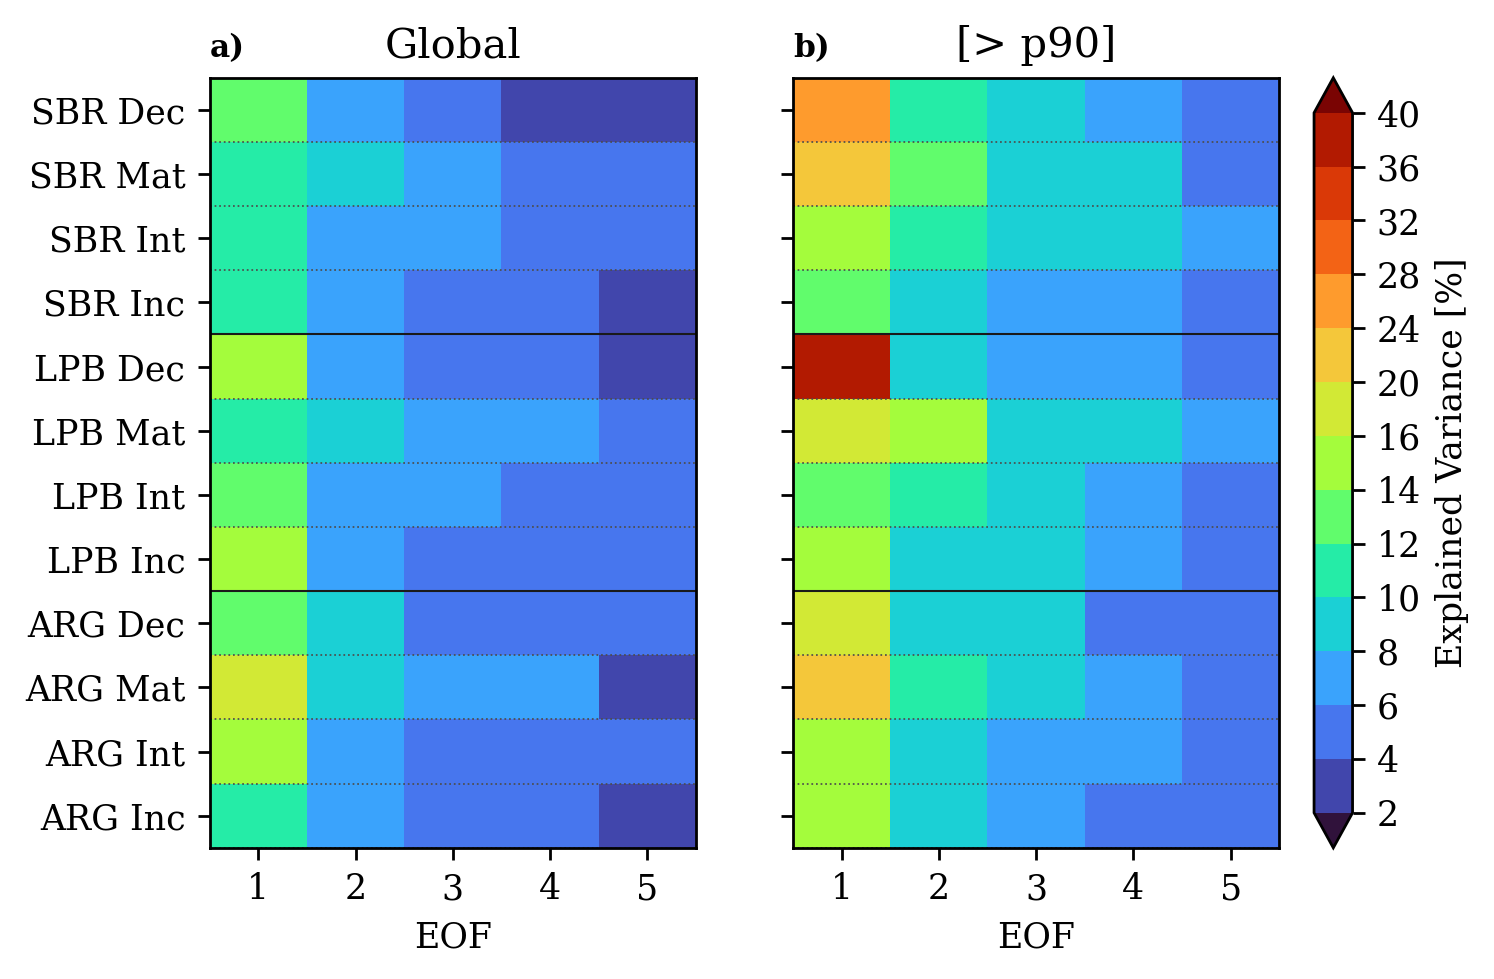
\includegraphics[width=0.8\textwidth]{images/tp/all_expvar_tp_mean2times.png}
\caption[Variância explicada pelos primeiros cinco modos (EOF1--EOF5) de precipitação]{Fracionamento da variância espacial total contida nos primeiros cinco modos dominantes (EOF1 a EOF5) do campo de precipitação total. Contrasta-se a distribuição da variância da População Global frente ao subconjunto de intensidade (p90) ao longo do ciclo de vida para cada região de ciclogênese.}
\label{fig:var_exp_tp}
\end{figure}

A Figura~\ref{fig:var_exp_tp} apresenta a distribuição percentual da variância espacial explicada pelos cinco primeiros modos empíricos (EOF1 a EOF5). As colunas contrastam a População Global (painel a) e o subconjunto de intensidade extrema (p90, painel b); as linhas correspondem às doze combinações de região de ciclogênese e fase evolutiva. A escala cromática quantifica a porcentagem de variância explicada. Os tons frios indicam modos dispersos; os quentes, alta concentração no modo principal.

Na População Global (painel a), o espectro de variância apresenta tons frios entre os cinco modos em todas as regiões e fases. O EOF1 explica entre 11.1\% e 16.4\% da variância total. Em SBR oscila entre 11.3\% (maturidade) e 13.8\% (decaimento), sem fase dominante. LPB apresenta seu máximo em incipiente (14.4\%) e decaimento (14.3\%), com a maturidade como mínimo (11.8\%). ARG exibe o comportamento mais distintivo. O EOF1 alcança seu máximo na maturidade (16.4\%), superando a intensificação (15.6\%), indicando um modo dominante bem diferenciado em relação a SBR e LPB. Os três primeiros modos explicam em conjunto, na maturidade, aproximadamente 26.8\% (SBR), 28.2\% (LPB) e 31.6\% (ARG) da variância total, o que indica que a maior parte da variabilidade pluviométrica não é capturada por alguns poucos modos ortogonais.

Esse reparto contrasta com o do vento, cujo EOF1 explica entre 30.9\% e 57.4\% na População Global (Seção~\ref{sec:var_exp_wind10}), e é consistente com a natureza discontínua da precipitação. Segundo \citet{hannachi2007empirical} (Seção~\ref{subsec:tb_eof}), quando a variância se reparte entre vários modos de valores próximos, o campo requer vários modos para reconstruir sua variabilidade.

Em contraste, o subconjunto p90 concentra a variância explicada pelo EOF1 nas fases tardias, com incrementos sistemáticos em relação à População Global que se intensificam até o final. Esse comportamento é oposto ao do vento, onde a filtragem p90 reduz a variância explicada pelo EOF1 em relação à População Global (25.4\%--37.6\% frente a 30.9\%--57.4\%; Seção~\ref{sec:var_exp_wind10}). Em SBR, o EOF1 passa de 11.3\% (População Global, maturidade) para 21.4\% (p90, maturidade) e de 13.8\% para 26.2\% no decaimento (saltos de 10.1 e 12.4 pontos).

Em LPB, o incremento já é notável na maturidade (11.8\% para 16\%, $+$4.2 pontos), mas é maior no decaimento (14.3\% para 36.5\%, $+$22.2 pontos). ARG mostra os incrementos mais moderados ($+$4.3 pontos na maturidade, $+$6.8 no decaimento). Em conjunto, os três primeiros modos de p90 explicam aproximadamente 43.8\% (SBR), 40.8\% (LPB) e 40.4\% (ARG) da variância na maturidade, frente a 26.8\%, 28.2\% e 31.6\% da População Global, confirmando que a filtragem dos 10\% mais intensos aumenta a organização espacial da variabilidade.

O comportamento distintivo de p90 durante o decaimento, onde o EOF1 concentra até 36.5\% da variância em LPB, poderia refletir que uma mesma estrutura espacial se repete em muitos casos, de modo que um único modo concentra mais de um terço da variância total do campo.

Na População Global, ARG apresenta maior variância explicada pelo EOF1 do que SBR durante a intensificação (15.6\% frente a 11.7\%), mas não na fase incipiente, onde registra o valor mais baixo da figura (11.1\%). Os maiores incrementos de p90 em relação à População Global ocorrem em SBR e LPB na maturidade e no decaimento.

Isso revela que a resposta da precipitação na População Global é difusa, justificando a necessidade de reter múltiplos modos; mas mostra também que os p90 têm a capacidade de organizar as precipitações em geometrias coerentes, um comportamento sem equivalente nos campos de vento.

%%%%%%%
\subsection{EOF1 na População Global}\label{subsec:eof1_tp_global}

\begin{figure}[htbp]
\centering
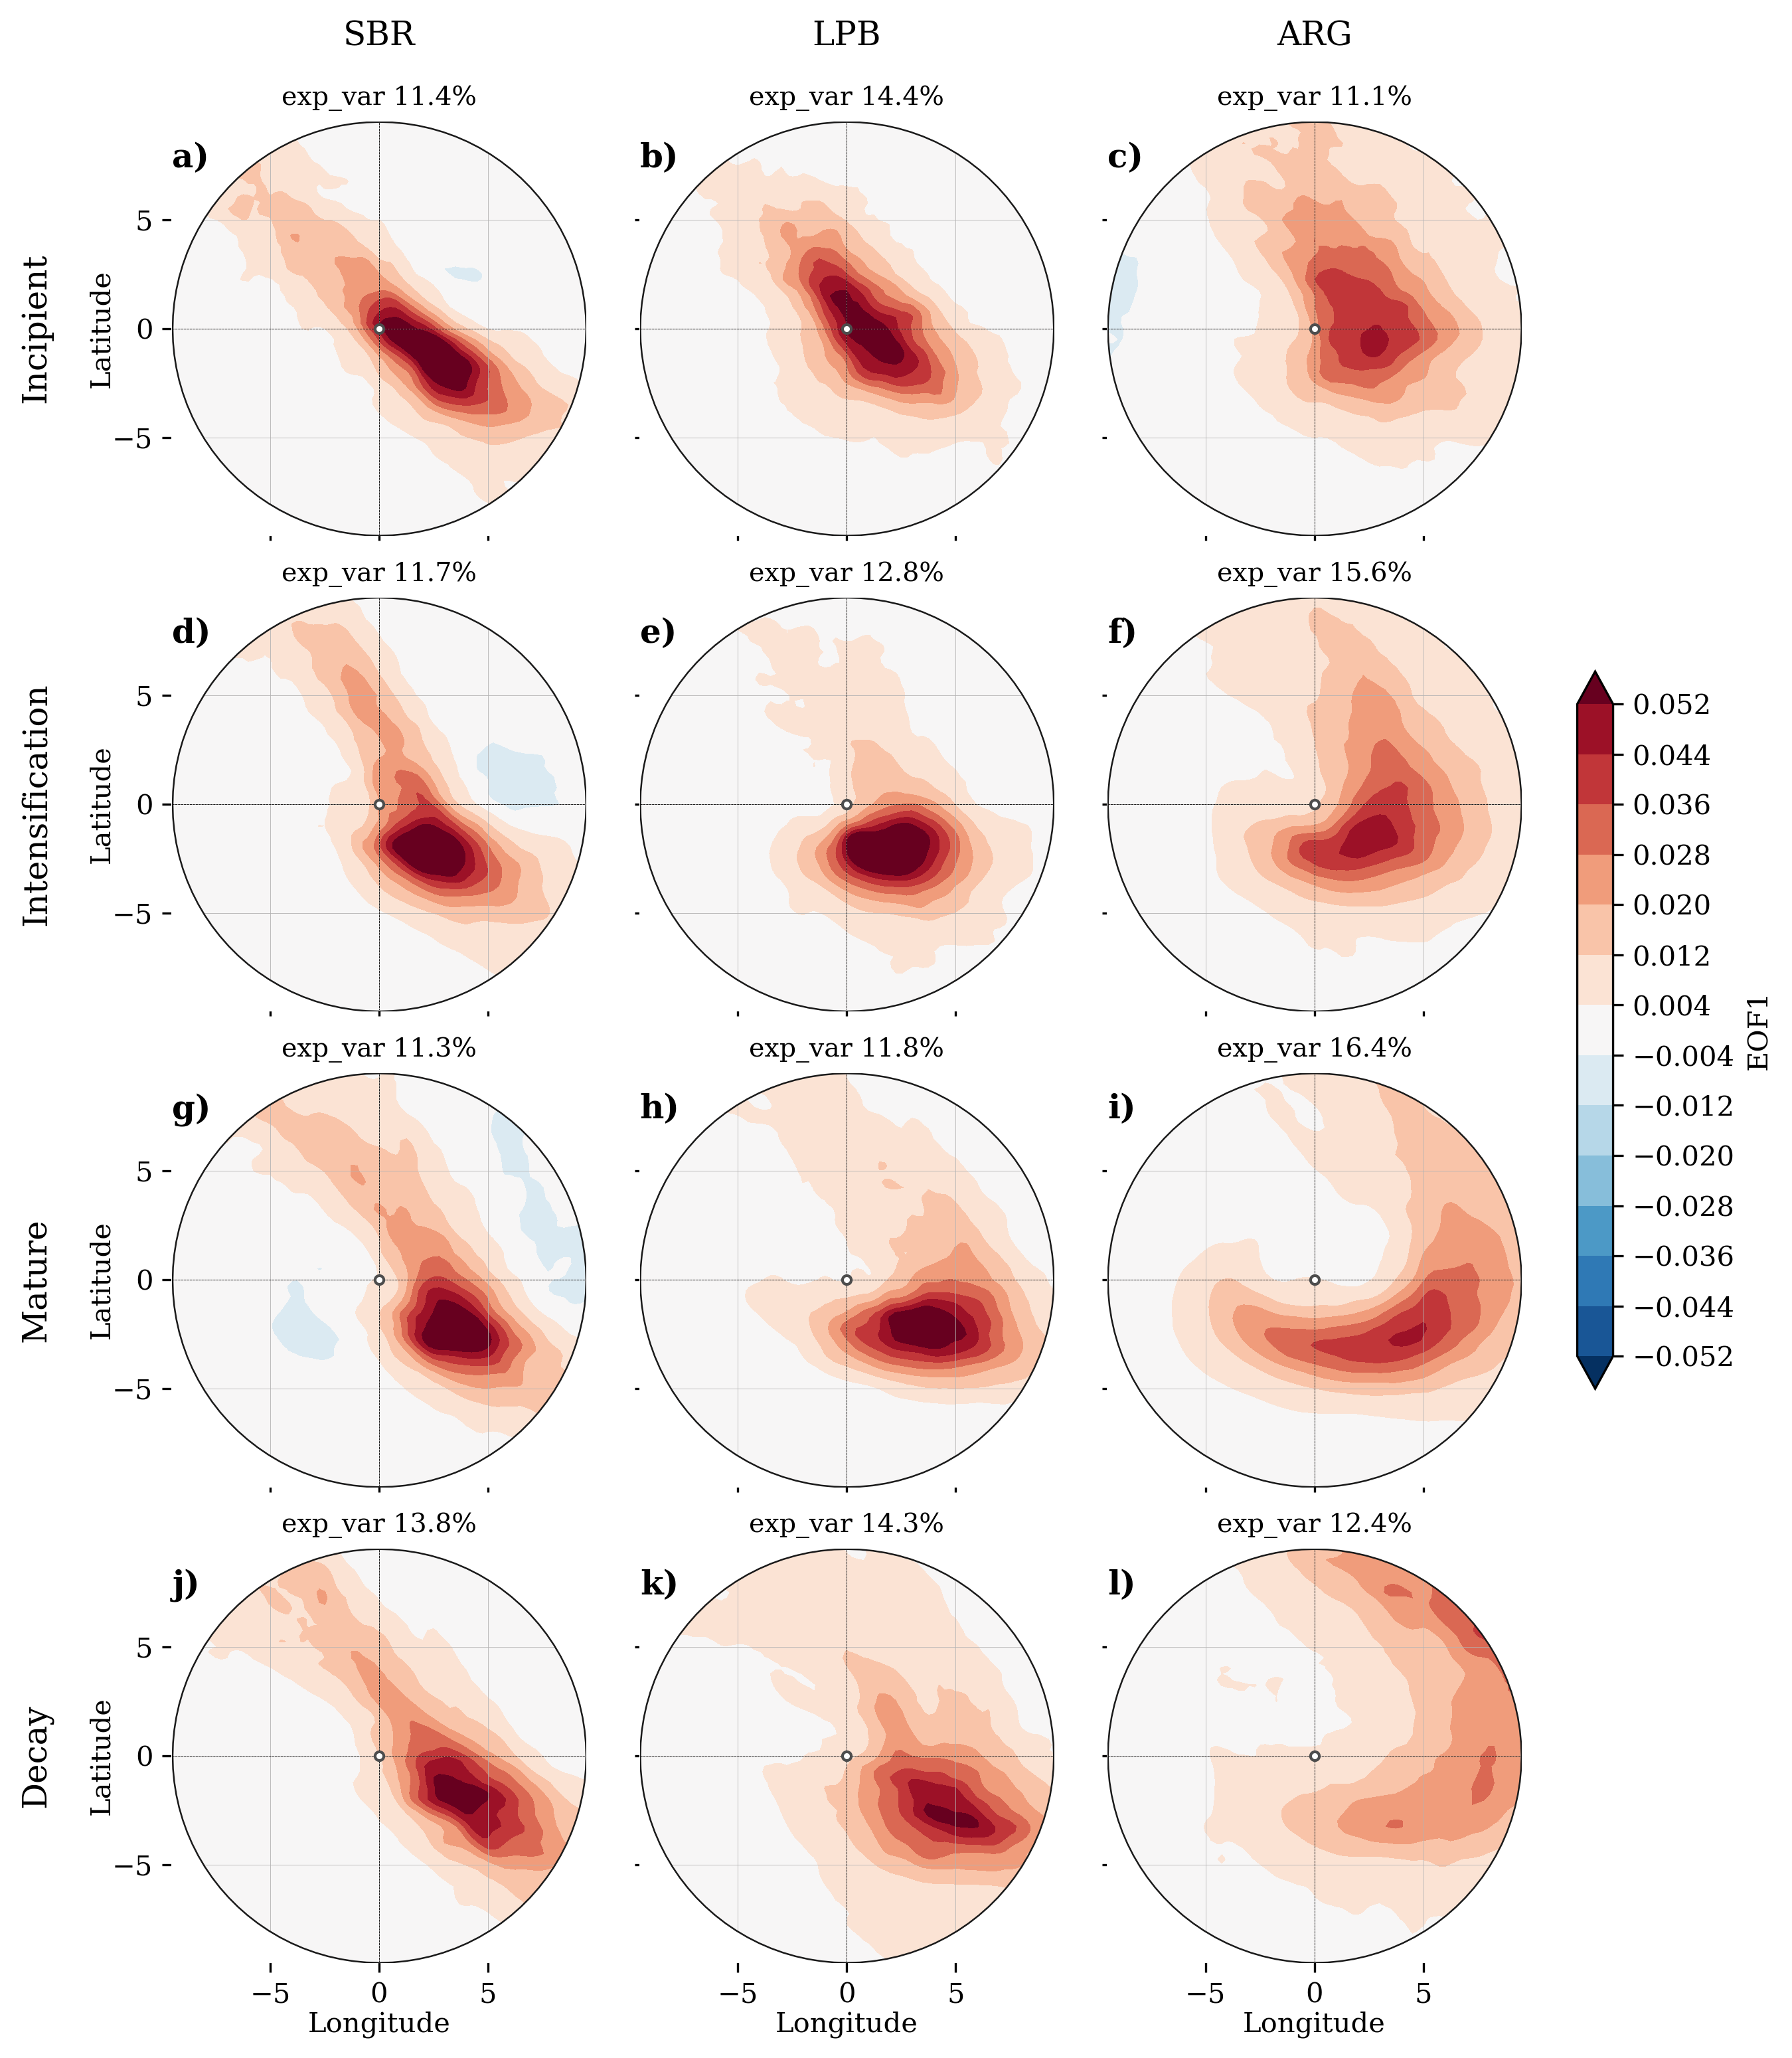
\includegraphics[width=\textwidth]{images/tp/pca1_tp_global_fasesxreg.png}
\caption[EOF1 de precipitação total (População Global)]{Primeiro modo espacial (EOF1) da precipitação total (mm/h) para a População Global de referência. A disposição matricial organiza a evolução por regiões de ciclogênese em colunas (SBR, LPB e ARG) e as fases de desenvolvimento evolutivo em linhas (Incipiente, Intensificação, Maturidade e Decaimento). Sobre cada painel se indica a porcentagem da variância espacial total explicada (\textit{exp\_var}) por essa componente principal. A escala cromática divergente quantifica as anomalias estruturais relativas ao centro do vórtice.}
\label{fig:eof1_tp_global}
\end{figure}

A Figura~\ref{fig:eof1_tp_global} apresenta os padrões espaciais do primeiro modo empírico (EOF1) da precipitação total, com a mesma disposição matricial dos campos PDFe anteriores, um domínio circular centrado no ciclone de 20 graus com contornos que representam anomalias estruturais em relação à média. As porcentagens de variância explicada oscilam entre 11.1\% e 16.4\%, o que indica uma menor dominância do primeiro modo do que no vento a 10~metros.

Em SBR, o EOF1 mantém uma estrutura consistente ao longo do ciclo de vida, com um núcleo positivo máximo ($\sim$0.052) ancorado no quadrante sudeste e uma cauda alongada em direção ao noroeste, formando uma faixa diagonal que atravessa o domínio, a mesma orientação do WCB descrita na Seção~\ref{subsec:kde_tp_global}.

Na fase incipiente (painel a, 11.4\%), o núcleo sudeste coexiste com a cauda noroeste e pequenas zonas negativas ($\sim$$-$0.004 a $-$0.012) no leste. Na intensificação (painel d, 11.7\%), os contornos se tornam mais simétricos e aparece maior área negativa no nordeste, com pequenas zonas negativas fracas. Na maturidade (painel g, 11.3\%), o núcleo positivo se afasta da origem em direção ao sudeste, com valores negativos a oeste e nordeste, também fracos e de pouca extensão. O decaimento (painel j, 13.8\%) mostra aumento de variância e desaparecimento dos valores negativos, resultando em um monopolo positivo puro alongado diagonalmente.

LPB apresenta os padrões mais simétricos e compactos. Na fase incipiente (painel b, 14.4\%), o núcleo positivo máximo ($\sim$0.052) forma uma faixa diagonal noroeste-sudeste, sem valores negativos; sua maior variância nessa fase (14.4\% frente a 11.4\% de SBR e 11.1\% de ARG) indica um modo dominante mais robusto e reprodutível. Na intensificação (painel e, 12.8\%), o núcleo migra para o sudeste com contornos quase perfeitamente simétricos, a simetria mais notável da fase. Na maturidade (painel h, 11.8\%), o núcleo se desloca ligeiramente para leste com contornos alongados. O decaimento (painel k, 14.3\%) mostra aumento de variância, com o núcleo a sudeste e uma cauda positiva em direção ao norte.

ARG exibe o comportamento mais distintivo e assimétrico. Na fase incipiente (painel c, 11.1\%), o núcleo positivo ($\sim$0.052) se localiza no sudeste com elongação ao norte e um dipolo fraco a oeste; sua variância é a mais baixa da figura, refletindo a alta variabilidade não estruturada da região nessa fase, coerente com a estrutura bimodal (núcleo sudeste e foco secundário noroeste) que o PDFe já mostrava para ARG incipiente (Seção~\ref{subsec:kde_tp_global}). A intensificação (painel f, 15.6\%) apresenta o valor mais alto dessa fase na População Global, com o núcleo sudeste mantendo sua posição deslocada e uma cauda norte ausente em SBR e LPB. Diferentemente das regiões oceânicas, em ARG o modo dominante permanece inclinado para o flanco dianteiro mesmo na intensificação. A maturidade (painel i, 16.4\%) alcança o máximo absoluto da figura global, único entre as três regiões, SBR e LPB têm seu pico no decaimento e na fase incipiente, respectivamente, indicando uma organização espacial excepcionalmente reprodutível na Argentina; o núcleo já adota aqui uma forma de arco, que se acentuará no subconjunto p90 (Seção~\ref{subsec:eof1_tp_p90}). O decaimento (painel l, 12.4\%) mostra valores positivos difusos sobre o semicírculo leste sem núcleo definido, contrastando com os padrões mais estruturados de SBR e LPB.

A faixa de anomalias positivas orientada noroeste-sudeste que mostra o EOF1 coincide com a posição dos máximos da PDFe (Seção~\ref{subsec:kde_tp_global}). As anomalias são mais intensas e concentradas em SBR e LPB do que em ARG, o que concorda com a maior intensidade da precipitação nessas regiões (Seção~\ref{sec:pdf_tp}).
Essa baixa variância explicada pelo primeiro modo, consistente com a natureza discontínua da precipitação (Seção~\ref{subsec:var_exp_tp}), constitui a linha de base dispersa que permite dimensionar a transformação estrutural que os eventos p90 experimentam ao se ocluir, quando abandonam esse comportamento transitório para confinar a precipitação em geometrias estruturadas, como se examina a seguir.

\subsection{EOF1 no subconjunto p90}\label{subsec:eof1_tp_p90}

\begin{figure}[htbp]
\centering
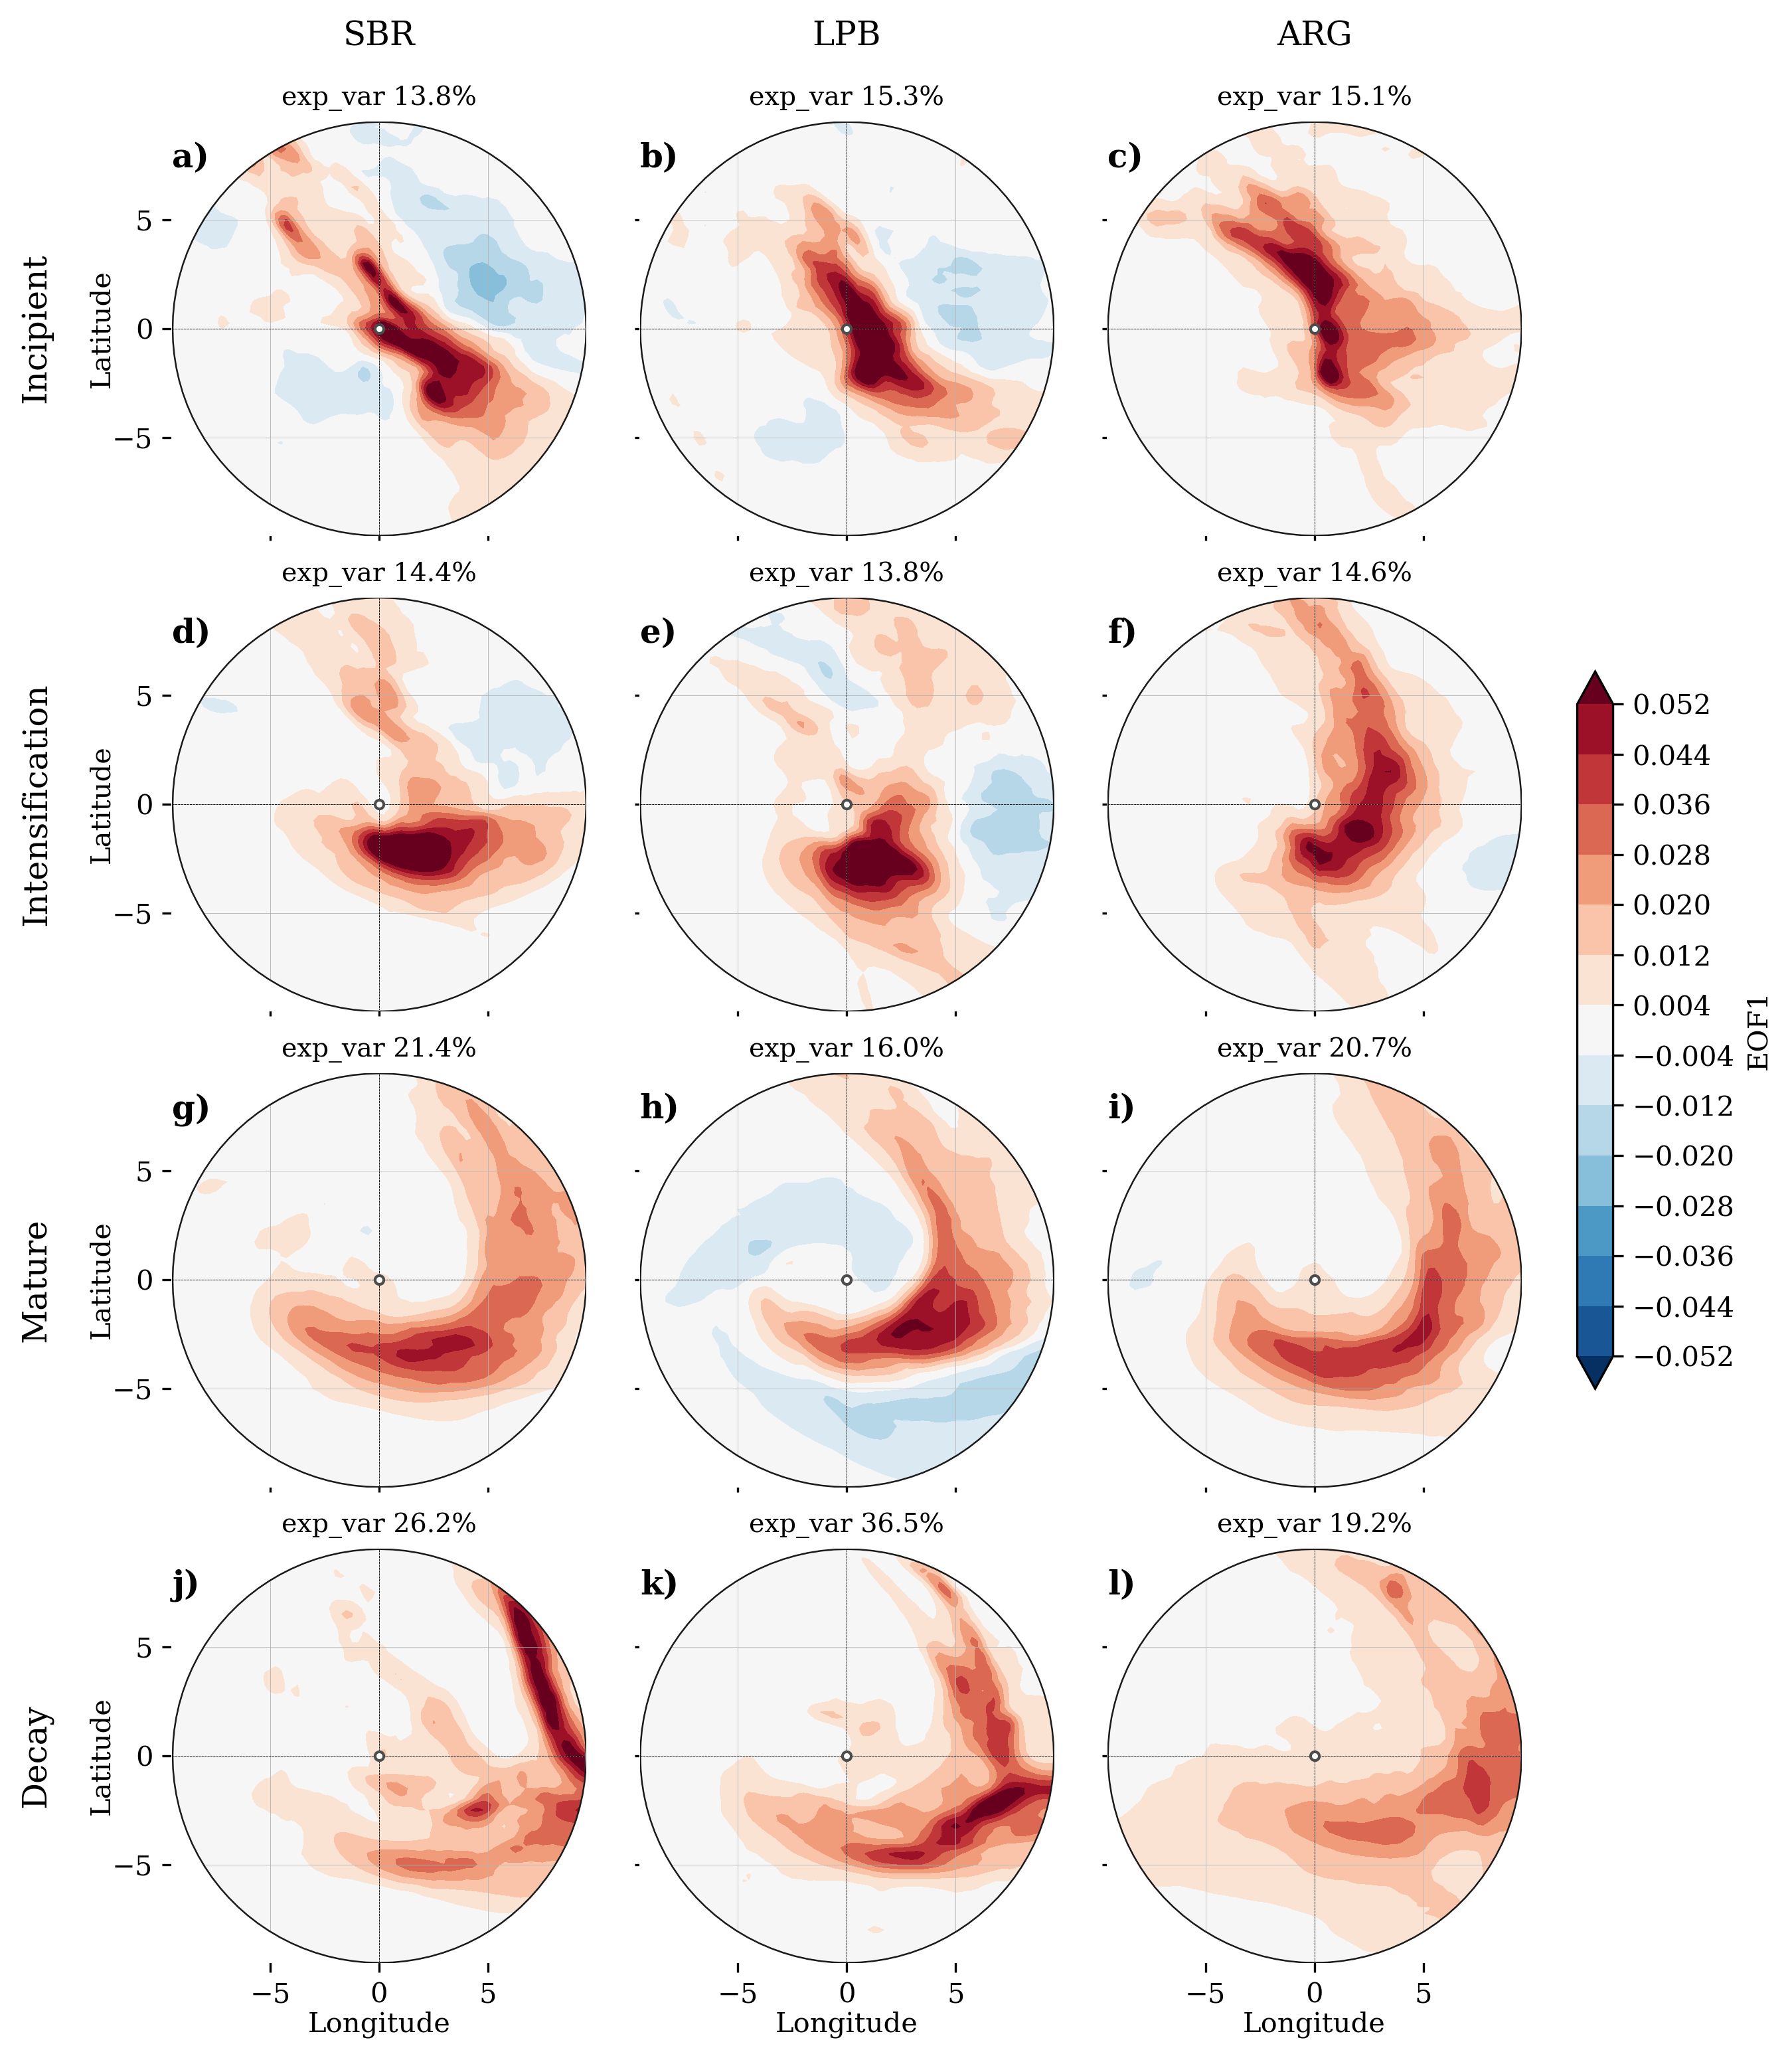
\includegraphics[width=\textwidth]{images/tp/pca1_tp_p90_fasesxreg.png}
\caption[EOF1 de precipitação total (subconjunto p90)]{Primeiro modo espacial (EOF1) da precipitação total (mm/h) para o estrato de ciclones intensos (percentil 90). O formato dos painéis (a--l), a nomenclatura de variância explicada e o domínio espacial mantêm uma correspondência estrita com a Figura~\ref{fig:eof1_tp_global}, permitindo quantificar a profunda transformação estrutural que os sistemas severos experimentam, especialmente durante sua oclusão final.}
\label{fig:eof1_tp_p90}
\end{figure}

A Figura~\ref{fig:eof1_tp_p90} apresenta os padrões espaciais do primeiro modo para o estrato p90, com a mesma disposição matricial da População Global. O contraste com a Figura~\ref{fig:eof1_tp_global} é imediato. A filtragem p90 produz dois efeitos sistemáticos em quase todas as regiões e fases (exceto ARG na intensificação): um incremento generalizado da variância explicada pelo EOF1, mais pronunciado nas fases tardias, e uma transformação morfológica que converte os monopolos e dipolos da população geral em estruturas em arco durante a maturidade e o decaimento.

Durante as fases iniciais, a filtragem p90 refina os padrões do global sem transformá-los radicalmente. Em SBR, a incipiente (painel a, 13.8\%, $+$2.4 pontos) mostra uma faixa diagonal noroeste-sudeste com zonas negativas ($\sim$$-$0.012 a $-$0.028) no nordeste, formando um dipolo mais nítido; a intensificação (painel d, 14.4\%, $+$2.7 pontos) mantém o núcleo próximo à origem, mais compacto, com a zona negativa melhor delimitada. Em LPB, a incipiente (painel b, 15.3\%, $+$0.9 pontos) mantém a faixa diagonal, mais estreita, com zonas negativas semelhantes; a intensificação (painel e, 13.8\%, $+$1.0 pontos) muda de monopolo compacto para dipolo, com o polo positivo ainda a sudeste. Em ARG, a incipiente (painel c, 15.1\%, $+$4.0 pontos) mostra a simplificação mais notável. A faixa diagonal é mais definida do que no global e desaparece o dipolo fraco; a intensificação (painel f, 14.6\%, $-$1.0 pontos) mantém o núcleo sudeste com a cauda norte, com valores negativos mínimos ausentes no global. A intensificação é, em conjunto, a fase mais estável entre global e p90, consistente com a simetria já observada entre ambas as populações no PDFe dessa mesma fase (Seção~\ref{subsec:kde_tp_p90}), o que sugere que os mecanismos de organização durante o desenvolvimento ativo não diferem qualitativamente entre sistemas ordinários e mais intensos.

A maturidade é onde ocorre a transformação morfológica mais drástica. Em SBR (painel g, 21.4\%, $+$10.1 pontos), o padrão do global é substituído por um monopolo positivo em arco do sudoeste até o nordeste, com o quadrante noroeste livre de anomalias positivas, primeira manifestação clara da estrutura em arco como modo dominante. LPB (painel h, 16.0\%, $+$4.2 pontos) forma um arco que envolve o sistema do sudoeste até o nordeste, com zonas negativas ($\sim$$-$0.008 a $-$0.024) no sul e sudeste. ARG (painel i, 20.7\%, $+$4.3 pontos) apresenta um arco semelhante mas de menor extensão e valores negativos mínimos, resultando em um monopolo arqueado sem dipolaridade.

No decaimento, as estruturas se distorcem e se deslocam para o flanco oriental externo. Em SBR (painel j, 26.2\%, $+$12.4 pontos), o núcleo positivo se concentra em uma faixa que margeia o extremo leste do domínio. LPB (painel k, 36.5\%) mostra um arco em forma de "L" invertido do sul até o leste. ARG (painel l, 19.2\%, $+$6.8 pontos) apresenta o padrão mais difuso da linha, semelhante em morfologia ao global, uma desorganização espacial que contrasta com a magnitude, muito mais concentrada. O próprio subconjunto p90 de ARG alcança aqui sua densidade de probabilidade mais alta de toda a Figura~\ref{fig:pdf_tp} (Seção~\ref{sec:pdf_tp}), o que indica que a concentração de magnitude e a organização espacial não são a mesma propriedade.

As estruturas em arco do EOF1 abrangem a zona onde a PDFe localiza os máximos de p90 (Seção~\ref{subsec:kde_tp_p90}), e apareceriam como o padrão dominante de variabilidade espacial se a intrusão seca desloca a umidade do núcleo para a periferia. O EOF1 a quantifica em 21.4\% (SBR) e 20.7\% (ARG) da variância total na maturidade, e 36.5\% (LPB) no decaimento, o que mostra que essa geometria se repete de forma consistente e não se deve a alguns poucos casos isolados.

Ao contrastar com o vento a 10~m, na maturidade os máximos de vento de p90 se concentram no quadrante noroeste, a ${\sim}$2--4° do centro (Seção~\ref{sec:kde_espacial_p90}), enquanto os máximos de precipitação se localizam a leste e sudeste, a ${\sim}$3.5--7° do centro (Seção~\ref{subsec:kde_tp_p90}). Essa separação entre os setores de máximo vento e máxima precipitação é um dos resultados centrais deste capítulo para os ciclones mais intensos.

\subsection{Significância estatística}\label{subsec:significancia_tp}

Para distinguir os sinais físicos das flutuações devidas à amostragem, avalia-se a significância estatística dos padrões espaciais mediante o método Bootstrap-t (Seção~\ref{subsec:bootstrap_significancia}). Como no vento, a análise se concentra na fase de maturidade, que apresenta o maior sinal dinâmico e é a de maior interesse para esta tese. A Figura~\ref{fig:xeof_madurez_global_tp} mostra os três primeiros modos (EOF1--EOF3) e suas componentes principais (PC1--PC3) para a População Global na maturidade, e a Figura~\ref{fig:xeof_madurez_p90_tp} apresenta a análise equivalente para p90. O hachurado indica as áreas significativas a 95\% de confiança.

\begin{figure}[htbp]
\centering
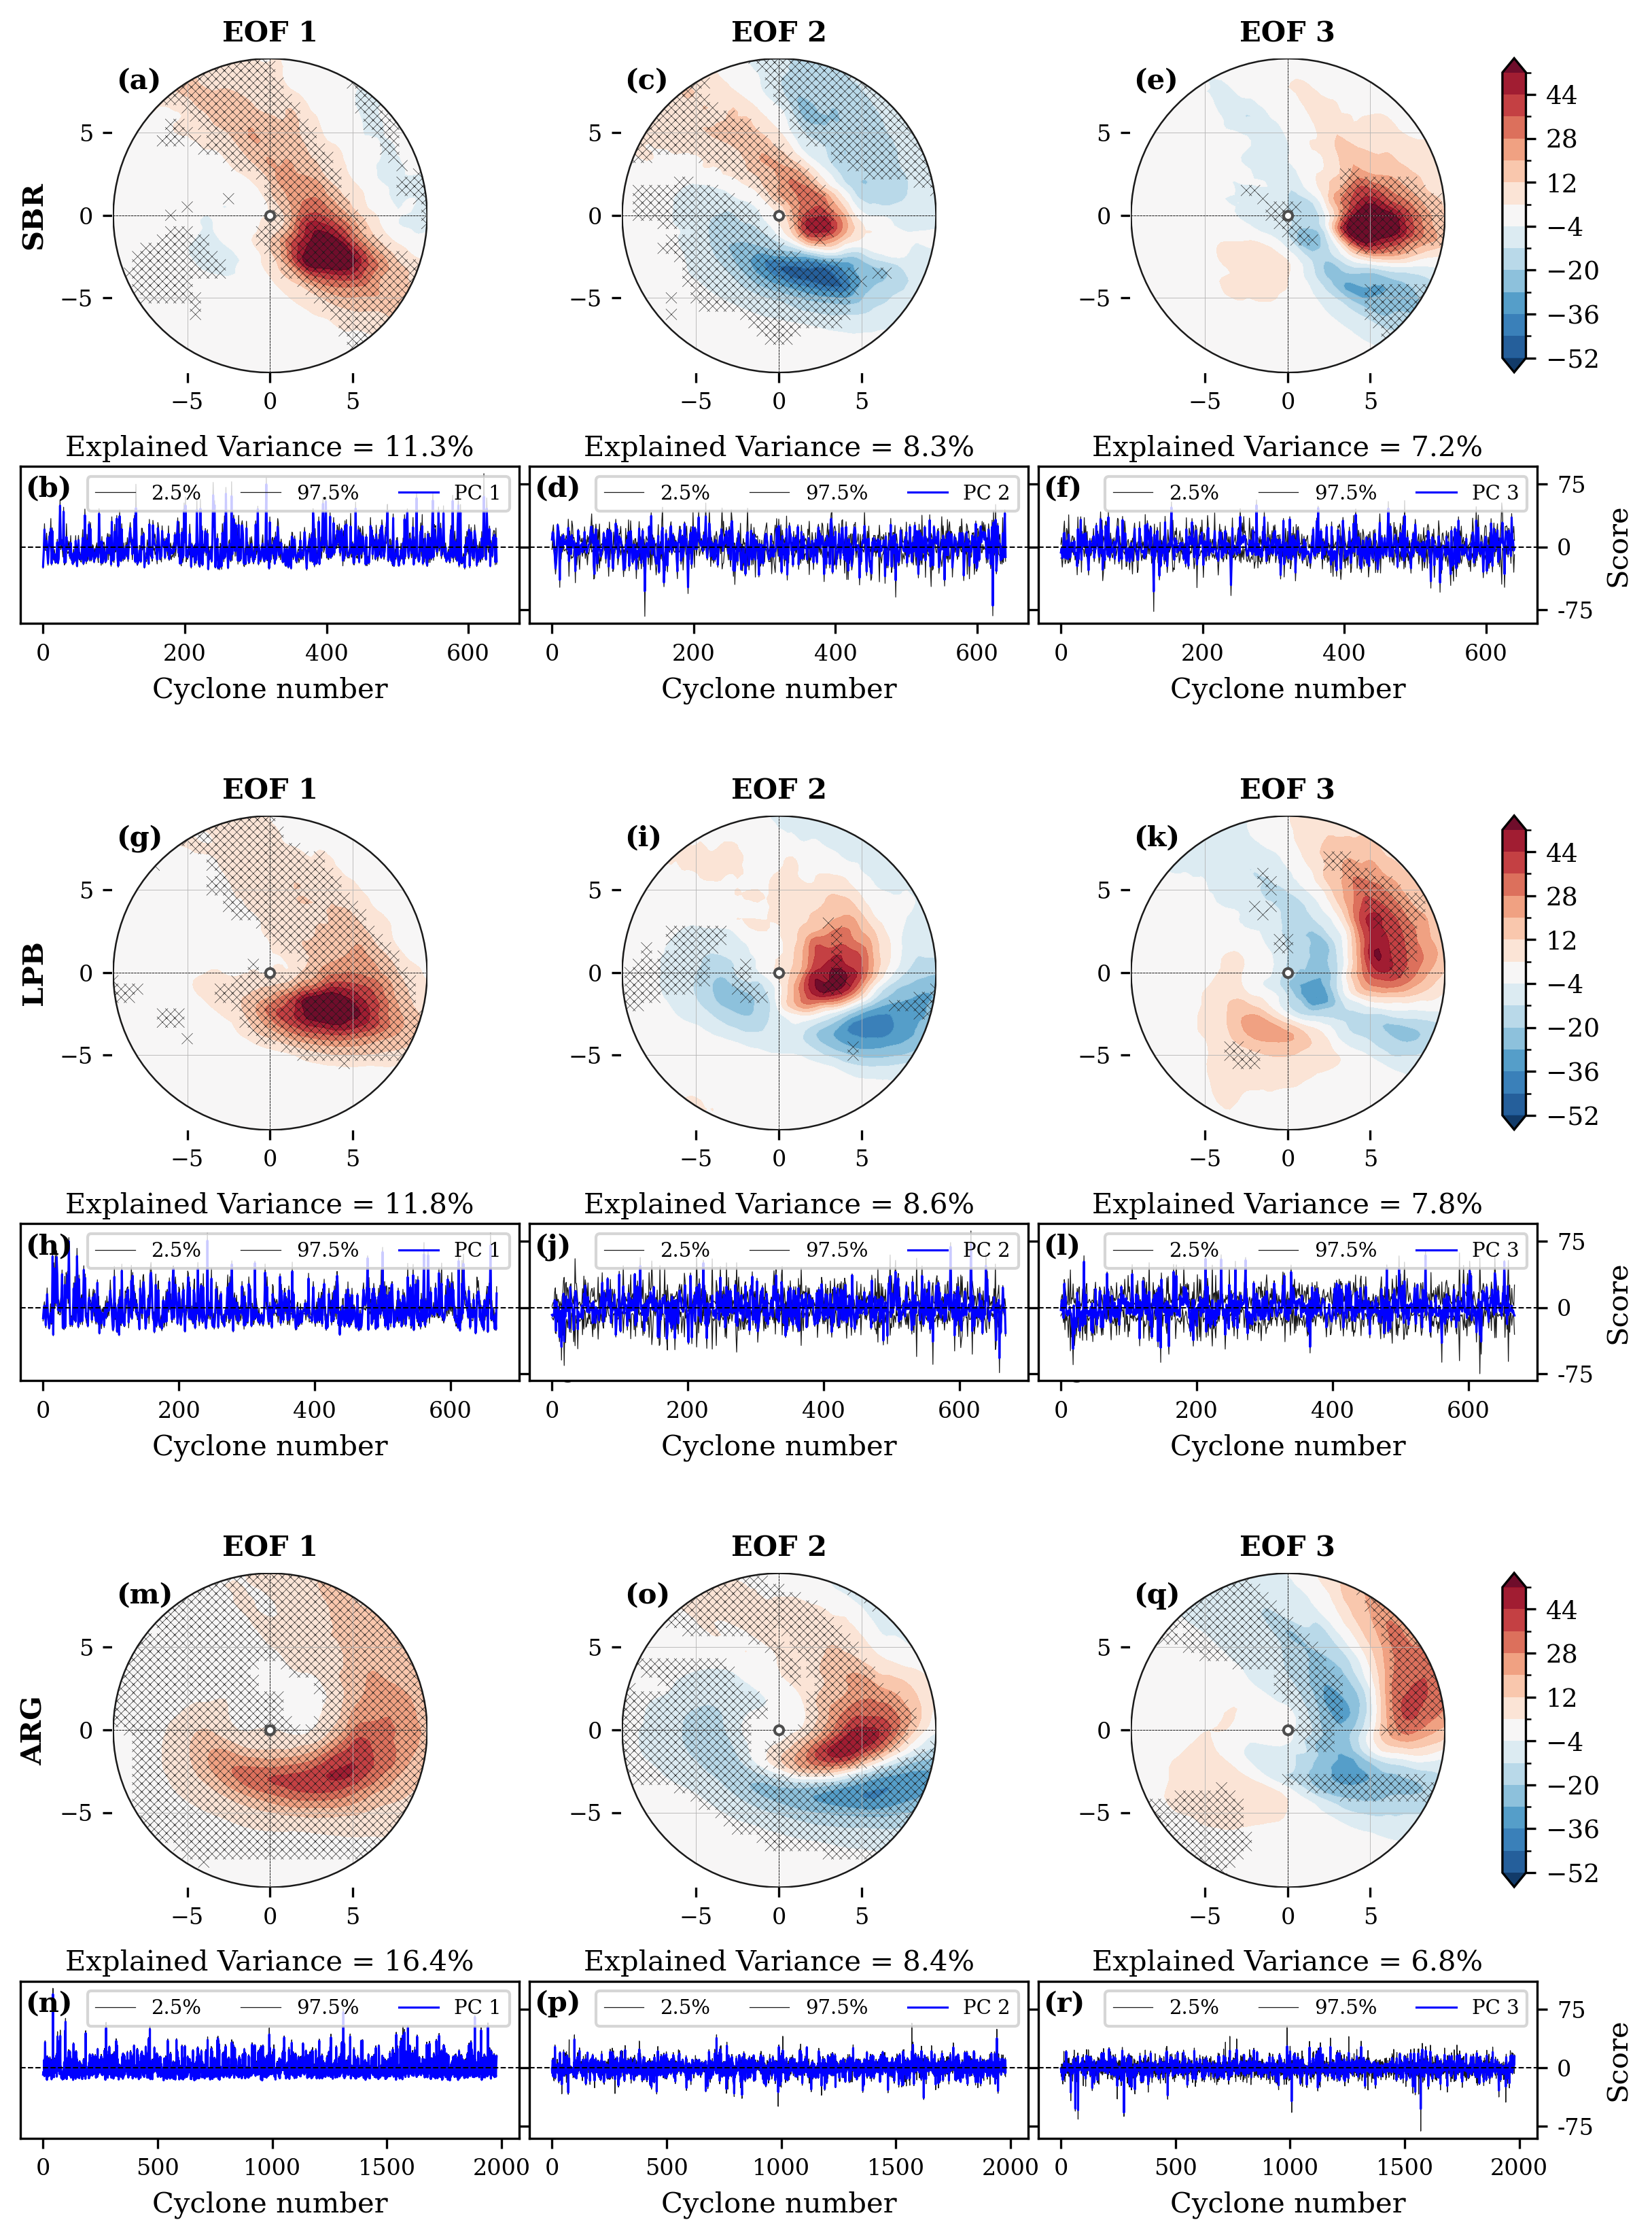
\includegraphics[width=\textwidth]{images/tp/xeof_global_tp_mature.png}
\caption[Significância espacial dos EOFs de precipitação em fase de maturidade (População Global)]{Decomposição EOF da precipitação total para a População Global em fase de maturidade. Painéis (a, g, m): mapas de EOF1 para SBR, LPB e ARG respectivamente; (c, i, o): EOF2; (e, k, q): EOF3. O hachurado indica significância estatística a 95\% (teste Bootstrap-t; Seção~\ref{subsec:bootstrap_significancia}). Painéis (b, h, n): componentes principais PC1; (d, j, p): PC2; (f, l, r): PC3. A linha cinza delimita os percentis 2.5 e 97.5 da distribuição bootstrap.}
\label{fig:xeof_madurez_global_tp}
\end{figure}

\begin{figure}[htbp]
\centering
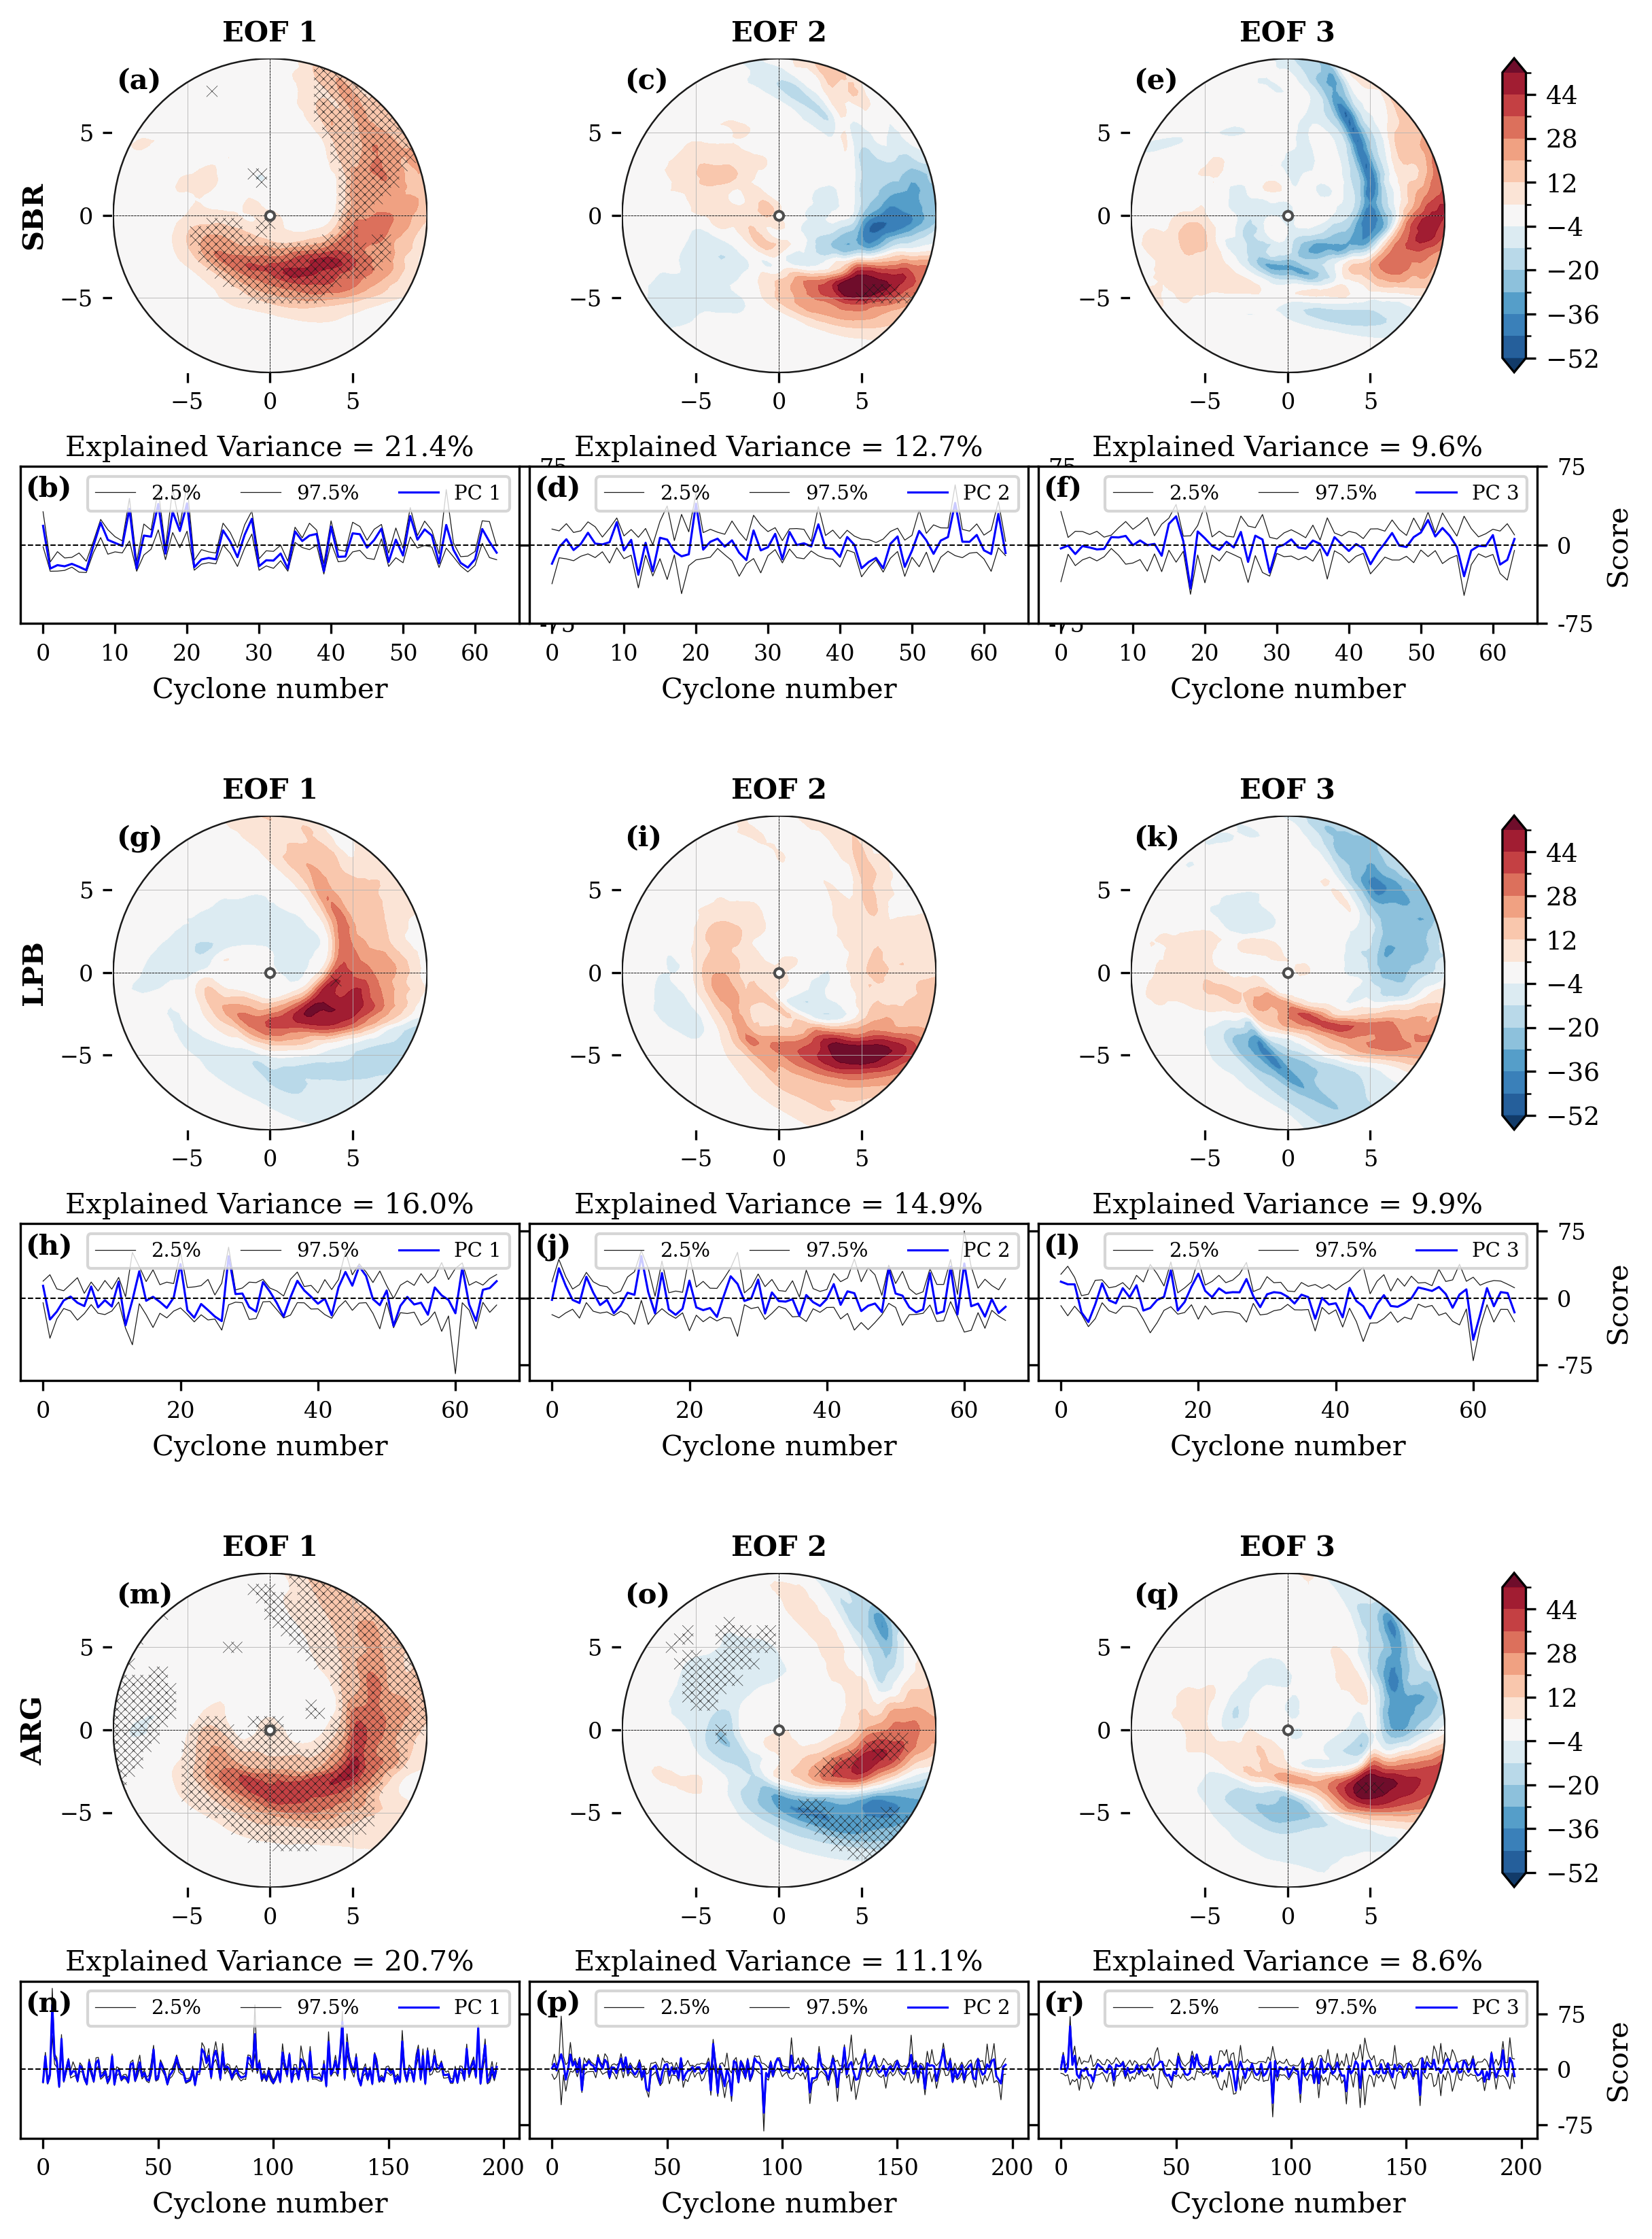
\includegraphics[width=\textwidth]{images/tp/xeof_p90_tp_mature.png}
\caption[Significância espacial dos EOFs de precipitação em fase de maturidade (subconjunto p90)]{Decomposição EOF da precipitação total para o subconjunto extremo (p90) em fase de maturidade. A disposição de painéis é idêntica à Figura~\ref{fig:xeof_madurez_global_tp}.}
\label{fig:xeof_madurez_p90_tp}
\end{figure}

A Figura~\ref{fig:xeof_madurez_global_tp} mostra que, para a População Global na maturidade, as áreas significativas do EOF1 se concentram sobre os valores positivos, sem se estender aos tons próximos de zero. Em SBR, o hachurado segue a faixa diagonal noroeste-sudeste, com alguma significância também no extremo negativo, perto do limite com os tons nulos. Em LPB, o hachurado se restringe à parte mais intensa dessa mesma faixa. Em ARG, o hachurado cobre praticamente todo o domínio, a cobertura mais ampla das três regiões, inclusive sobre tons positivos fracos.
Na Figura~\ref{fig:xeof_madurez_p90_tp}, SBR e ARG mostram um arco de significância denso, que traça a geometria do arco sudoeste-nordeste já identificado no EOF1 (Seção~\ref{subsec:eof1_tp_p90}), consistente com o salto na variância explicada dessa fase. LPB constitui uma excepção notável. Seu salto de variância explicada na maturidade (11.8\% para 16.0\%) é na realidade o mais moderado das três regiões nessa fase, frente aos $+$10.1 pontos de SBR; seu EOF1 carece de área significativa apreciável a 95\%, o que indica que a transformação morfológica em direção à faixa arqueada não é respaldada por um sinal estatisticamente robusto sob o teste Bootstrap-$t$, coerente com a densidade espacial mais baixa que LPB já mostrava no PDFe dessa mesma fase (${\approx}$7--9$\times10^{-4}$, a mais baixa da linha; Seção~\ref{subsec:kde_tp_p90}). As amplitudes de PC2 e PC3 alcançam ou superam em certos casos os limites de confiança bootstrap, o que sugere que mesmo a variabilidade secundária pode ser fisicamente relevante na maturidade dos sistemas mais intensos.

Na Figura~\ref{fig:xeof_madurez_global_tp}, os modos secundários também apresentam áreas significativas, embora de extensão mais limitada do que o EOF1. Em SBR, o EOF2 é significativo tanto em seu polo positivo quanto negativo, com hachurado denso onde o sinal é mais intenso; o EOF3 é significativo principalmente sobre o sinal positivo, com áreas menores perto do centro e no extremo sudeste. Em LPB, o EOF2 apresenta um hachurado mais restrito, limitado aos tons mais intensos do polo positivo e ausente no negativo; o EOF3 tem áreas pequenas que não coincidem com o sinal mais forte. Em ARG, o EOF2 é significativo em ambos os sinais exceto nos valores próximos de zero, e o EOF3 cobre uma área maior do que em LPB, sobre as regiões de sinal mais intenso.

Na Figura~\ref{fig:xeof_madurez_p90_tp}, por sua vez, os modos secundários perdem quase toda sua significância. Em SBR, o EOF2 só conserva uma área pequena perto de seu máximo positivo, e o EOF3 não apresenta áreas significativas. Em LPB, nem o EOF2 nem o EOF3 alcançam significância a 95\%, o que se soma à ausência já apontada em seu EOF1. Em ARG, o EOF2 mostra áreas hachuradas dispersas a noroeste e a sudeste, sem um padrão claro em relação ao sinal, e o EOF3 tampouco é significativo. Esse contraste indica que a filtragem p90, além de concentrar a variância no EOF1 (Seção~\ref{subsec:eof1_tp_p90}), reduz a robustez estatística dos modos secundários, com a possível exceção parcial de ARG.

Essa diferença é coerente com o já apontado para o EOF1 de LPB, cujo salto de variância explicada é o mais moderado das três regiões e cuja densidade espacial no PDFe dessa fase é a mais baixa (Seção~\ref{subsec:kde_tp_p90}), o que sugere um sinal mais fraco e, portanto, mais difícil de distinguir do ruído de amostragem sob o teste Bootstrap-$t$. Em síntese, a estrutura em arco de p90 é respaldada por um sinal estatisticamente robusto em SBR e ARG, mas em LPB continua sendo um padrão morfológico consistente sem confirmação como distinguível do ruído de amostragem.

%%%%%%%%%%%%%%
\section{Componentes principais (PC1--PC3)}\label{sec:dinamica_pc1_tp}

A fragmentação da variância documentada na maturidade e sua transformação em direção à coerência no decaimento têm sua contrapartida temporal no comportamento estatístico das Componentes Principais. Diferentemente do vento, onde as amplitudes de PC2 e PC3 são menores do que as de PC1 na População Global e PC2 se aproxima de PC1 em p90 (Seção~\ref{subsec:res_dinamica_pc1}), na precipitação as amplitudes de PC1, PC2 e PC3 não diferem muito entre si nem entre a População Global e p90. Na precipitação, a correlação entre PC1 e a vorticidade se debilita em magnitude durante a maturidade em LPB, até perder significância; em SBR perde magnitude nessa mesma fase mas se mantém significativa; enquanto em ARG se mantém significativa durante todo o ciclo, com magnitude que se fortalece e depois se debilita ao longo das fases (Seção~\ref{subsec:pc1_global_tp}).

\begin{table}[htbp]
\centering
\caption[Momentos estatísticos e correlação de PC1--PC3 de precipitação - População Global]
{Assimetria ($\gamma_1$) e curtose ($\gamma_2$) da PC1 de precipitação, e correlação de Spearman em valor absoluto ($|r|$) entre PC1, PC2 e PC3 e a vorticidade relativa a 850 hPa associada à fase, para a População Global. Reporta-se o valor absoluto porque o sinal da correlação depende da convenção de sinal arbitrária de cada EOF (Seção~\ref{subsec:analisis_pc}); o relevante é a magnitude da correlação e sua significância. Os valores significativos ($p<0.05$) são mostrados em negrito.}
\label{tab:stat_global_tp}
\begin{tabular*}{\textwidth}{@{\extracolsep{\fill}}llrrrrr}
\hline
\textbf{Região} & \textbf{Fase} & \textbf{Assimetria ($\gamma_1$)} & \textbf{Curtose ($\gamma_2$)} & \textbf{$|$PC1$|$} & \textbf{$|$PC2$|$} & \textbf{$|$PC3$|$} \\
\hline
\textbf{SBR} & Incipiente       & 1.12 & 1.58 & \textbf{0.52} & \textbf{0.16} & \textbf{0.26} \\
             & Intensificação & 0.85 & 0.87 & \textbf{0.52} & \textbf{0.13} & \textbf{0.46} \\
             & Maturidade         & 1.20 & 1.53 & \textbf{0.17} & \textbf{0.65} & 0.04 \\
             & Decaimento     & 1.49 & 2.18 & \textbf{0.19} & \textbf{0.15} & \textbf{0.29} \\
\hline
\textbf{LPB} & Incipiente       & 1.34 & 2.85 & \textbf{0.49} & \textbf{0.10} & 0.07 \\
             & Intensificação & 1.03 & 1.44 & \textbf{0.59} & 0.01 & \textbf{0.33} \\
             & Maturidade         & 1.09 & 1.45 & 0.04 & \textbf{0.61} & \textbf{0.34} \\
             & Decaimento     & 2.06 & 6.02 & 0.07 & \textbf{0.24} & \textbf{0.13} \\
\hline
\textbf{ARG} & Incipiente       & 2.55 & 9.30 & \textbf{0.51} & \textbf{0.18} & 0.04 \\
             & Intensificação & 1.52 & 4.06 & \textbf{0.66} & \textbf{0.26} & \textbf{0.22} \\
             & Maturidade         & 1.74 & 5.40 & \textbf{0.53} & \textbf{0.43} & 0.04 \\
             & Decaimento     & 2.50 & 9.59 & \textbf{0.25} & 0.00 & \textbf{0.13} \\
\hline
\end{tabular*}
\end{table}


\subsection{Relação com a intensidade na População Global}\label{subsec:pc1_global_tp}

A Tabela~\ref{tab:stat_global_tp} documenta a assimetria e a curtose da PC1, e a correlação de Spearman em valor absoluto entre PC1, PC2 e PC3 e a vorticidade relativa a 850~hPa associada à fase, para a População Global, desagregadas por região e fase.

A análise dos momentos estatísticos revela uma característica distintiva, a presença persistente de caudas pesadas (leptocurtose positiva) ao longo de todo o ciclo de vida. Diferentemente do vento, onde a curtose evoluía para valores próximos de zero ou negativos na maturidade, aqui se observam valores de $\gamma_2$ positivos nas três regiões: SBR oscila entre $+0.87$ (intensificação) e $+2.18$ (decaimento); LPB exibe curtose pronunciada na incipiência ($+2.85$) e no decaimento ($+6.02$); ARG apresenta os valores mais extremos, superiores a $+9$ tanto na incipiência quanto no decaimento. O sesgo positivo persistente ($\gamma_1 > +0.8$ em todos os casos) reflete a presença de eventos com anomalias pluviométricas intensas em relação ao padrão médio.

O exame das correlações entre PC1 e vorticidade revela uma evolução distinta por região durante a maturidade. Em SBR, a correlação moderada das fases iniciais ($|r|\approx0.52$) perde magnitude até a maturidade ($|r|=0.17$) e o decaimento ($|r|=0.19$), embora se mantenha significativa em ambas as fases. Em LPB, as correlações significativas durante o desenvolvimento ($|r|=0.49$ na incipiência, $0.59$ na intensificação) colapsam para valores não significativos na maturidade ($|r|=0.04$, $p=0.26$) e no decaimento ($|r|=0.07$, $p=0.07$). ARG mantém correlações significativas durante todo o ciclo, com um fortalecimento inicial até a intensificação ($|r|=0.66$) e um debilitamento posterior até o decaimento ($|r|=0.25$).

Esse comportamento reflete processos físicos diferenciados. Em SBR, a correlação perde magnitude até a maturidade e o decaimento, embora se mantenha significativa; em LPB, as correlações significativas do desenvolvimento colapsam para valores não significativos na maturidade e no decaimento. Em ARG, a correlação se mantém significativa durante todo o ciclo (Seção~\ref{subsec:pc1_global_tp}), o que é consistente com o fato de seu EOF1 ser, na População Global, o modo mais dominante e reprodutível das três regiões, com o máximo absoluto de variância explicada de toda a figura na maturidade (16.4\%, Seção~\ref{subsec:eof1_tp_global}). Em SBR e LPB, por sua vez, o EOF1 explica uma fração menor da variância justamente nessa fase (11.3\% e 11.8\%, respectivamente, Seção~\ref{subsec:var_exp_tp}), o que poderia tornar sua correlação com a vorticidade mais frágil.

O debilitamento de PC1 na maturidade não implica que a vorticidade deixe de organizar o campo de precipitação, em SBR e LPB o sinal de maior magnitude se desloca para PC2. Em SBR, PC2 alcança $|r|=0.65$ na maturidade, uma magnitude maior do que a do próprio PC1 nessa mesma fase ($|r|=0.17$); em LPB ocorre algo equivalente, PC2 chega a $|r|=0.61$ na maturidade, justamente quando PC1 perde significância ($|r|=0.04$). Esse revezamento entre modos sugere que, ao se ocluir o sistema e suprimir-se a convecção do núcleo, a parte da estrutura pluviométrica que continua escalando com a intensidade deixa de ser a dominante (EOF1) e passa a ser uma estrutura secundária (EOF2), sem que a correlação entre precipitação e vorticidade desapareça por completo.

\begin{table}[htbp]
\centering
\caption[Momentos estatísticos e correlação de PC1--PC3 de precipitação - Subconjunto p90]
{Assimetria ($\gamma_1$) e curtose ($\gamma_2$) da PC1 de precipitação, e correlação de Spearman em valor absoluto ($|r|$) entre PC1, PC2 e PC3 e a vorticidade relativa a 850 hPa associada à fase, para o subconjunto extremo (p90). Reporta-se o valor absoluto porque o sinal da correlação depende da convenção de sinal arbitrária de cada EOF (Seção~\ref{subsec:analisis_pc}); o relevante é a magnitude da correlação e sua significância. Os valores significativos ($p<0.05$) são mostrados em negrito.}
\label{tab:stat_p90_tp}
\begin{tabular*}{\textwidth}{@{\extracolsep{\fill}}llrrrrr}
\hline
\textbf{Região} & \textbf{Fase} & \textbf{Assimetria ($\gamma_1$)} & \textbf{Curtose ($\gamma_2$)} & \textbf{$|$PC1$|$} & \textbf{$|$PC2$|$} & \textbf{$|$PC3$|$} \\
\hline
\textbf{SBR} & Incipiente       & 1.57 & 3.48  & \textbf{0.36} & \textbf{0.53} & 0.22 \\
             & Intensificação & 1.20 & 1.67  & \textbf{0.48} & \textbf{0.43} & 0.24 \\
             & Maturidade         & 0.41 & -0.67 & 0.17 & 0.22 & 0.11 \\
             & Decaimento     & 4.02 & 19.77 & \textbf{0.34} & 0.17 & 0.18 \\
\hline
\textbf{LPB} & Incipiente       & 1.90 & 4.52  & \textbf{0.49} & \textbf{0.31} & 0.22 \\
             & Intensificação & 0.60 & -0.38 & \textbf{0.43} & 0.01 & \textbf{0.26} \\
             & Maturidade         & 0.56 & 0.16  & 0.03 & 0.18 & 0.02 \\
             & Decaimento     & 4.34 & 23.18 & \textbf{0.50} & 0.09 & 0.03 \\
\hline
\textbf{ARG} & Incipiente       & 4.43 & 30.88 & \textbf{0.44} & \textbf{0.29} & \textbf{0.23} \\
             & Intensificação & 1.87 & 5.15  & \textbf{0.37} & \textbf{0.21} & \textbf{0.28} \\
             & Maturidade         & 1.66 & 4.53  & \textbf{0.24} & 0.03 & 0.14 \\
             & Decaimento     & 1.96 & 3.37  & \textbf{0.39} & \textbf{0.32} & 0.10 \\
\hline
\end{tabular*}
\end{table}


\subsection{Relação com a intensidade no subconjunto p90}\label{subsec:pc1_p90_tp}

A Tabela~\ref{tab:stat_p90_tp} expõe os parâmetros estatísticos e as correlações (PC1--PC3, em valor absoluto) para o subconjunto extremo. Diferentemente da leptocurtose persistente da População Global, aqui se documenta uma evolução não monotônica em direção a valores extremos no decaimento, junto com um colapso da correlação de PC1 em SBR e LPB durante a maturidade.

Em SBR observa-se leptocurtose alta nas fases iniciais ($\gamma_2 = +3.48$ na incipiência, $+1.67$ na intensificação), seguida de uma curtose próxima de zero na maturidade ($\gamma_2 = -0.67$, sem caudas pronunciadas) e muito alta no decaimento ($\gamma_2 = +19.77$, $\gamma_1 = +4.02$). LPB reproduz esse padrão com valores ainda mais extremos: curtose de $+4.52$ na incipiência, próxima de zero na maturidade ($\gamma_2 = +0.16$) e superior a $+23$ no decaimento. ARG apresenta a curtose mais elevada do conjunto na incipiência ($\gamma_2 = +30.88$), com valores positivos durante todo o ciclo, embora decrescentes após essa fase ($+5.15$ na intensificação, $+4.53$ na maturidade, $+3.37$ no decaimento). Em ARG, essa curtose tão alta na fase incipiente é consistente com a maior heterogeneidade estrutural que caracteriza essa fase (Seção~\ref{subsec:tb_fases}), acentuada por um mecanismo de gênese a sotavento dos Andes (Seção~\ref{subsec:tb_arg}), mais variável do que o forçamento termodinâmico oceânico que organiza a gênese em SBR e LPB. A maioria dos sistemas incipientes de ARG projeta-se fracamente sobre o EOF1, enquanto alguns poucos casos, com amplitudes muito mais altas e alinhados com a geometria do modo dominante, geram a cauda pesada que eleva a curtose observada. Essa leitura é coerente com o apontado na Seção~\ref{subsec:eof1_tp_p90}, onde o EOF1 de ARG na fase incipiente de p90 apresenta o maior salto de variância explicada entre as três regiões nessa fase ($+$4.0 pontos) e perde o dipolo fraco presente na População Global, o que indica que a filtragem p90 retém principalmente os casos melhor alinhados com o modo dominante.

As correlações de PC1 com a vorticidade colapsam durante a maturidade em SBR ($|r|=0.17$, não significativo) e LPB ($|r|=0.03$, $p = 0.80$), recuperando-se no decaimento ($|r|=0.34$ e $0.50$ respectivamente), enquanto ARG mantém valores significativos ainda que atenuados ($|r|=0.24$ na maturidade).

Esse colapso é consistente com a defasagem de fases já documentada (Seção~\ref{sec:pdf_tp}). Em p90, o máximo de precipitação tende a ocorrer antes do máximo de intensidade dinâmica, e quando o vórtice alcança sua vorticidade extrema na maturidade, o núcleo poderia já ter secado pela chegada de ar subsidente, como se propôs nessa mesma seção, de modo que a vorticidade extrema já não coincidiria temporalmente com uma fase ativa de geração de precipitação.

Os modos secundários em p90 não reproduzem o padrão de revezamento observado na População Global. PC2 é significativo principalmente nas fases iniciais (incipiente e intensificação) nas três regiões, com magnitudes de $|r|$ entre $0.32$ e $0.53$, mas não recupera especificamente o sinal que PC1 perde na maturidade. Isso sugere que, nos sistemas mais intensos, o debilitamento do vínculo entre precipitação e vorticidade durante a maturidade é mais generalizado do que na População Global, sem que um único modo secundário assuma o papel que PC1 deixou.

Em SBR e LPB, a perda de correlação durante a maturidade ocorre ao mesmo tempo que a separação espacial documentada nas seções anteriores. Uma vez que a estrutura em arco domina o campo, a amplitude da PC1 já não depende da profundidade do vórtice, mas de quanto dessa faixa permanece dentro do domínio centrado no sistema à medida que o ciclone se dissipa, o que poderia explicar a evolução para a normalidade estatística na maturidade seguida da curtose muito alta no decaimento. Essa hipótese é coerente com a localização dos núcleos de p90 nessas fases (Seção~\ref{subsec:kde_tp_p90}), que na maturidade se situam perto da borda do domínio em SBR (${\sim}$6--7° a leste) e no decaimento se afastam ainda mais, com os contornos de LPB alcançando $+$9° de longitude, praticamente o limite do domínio de 20°×20°. Em LPB essa leitura deve ser tomada com cautela, pois, diferentemente de SBR, sua estrutura em arco em p90-maturidade é morfologicamente clara mas não alcança significância estatística a 95\% (Seção~\ref{subsec:significancia_tp}), de modo que o mecanismo proposto descreve um padrão consistente antes do que uma estrutura já confirmada como robusta frente à amostragem.

A persistência de correlações significativas em ARG durante toda a evolução é consistente com a maior dominância e reprodutibilidade de seu EOF1 já apontadas (Seção~\ref{subsec:pc1_global_tp}), e com a menor magnitude de precipitação de ARG em relação a SBR e LPB já documentada no PDF (Seção~\ref{sec:pdf_tp}).
Esses resultados mostram que o campo de precipitação é estruturalmente mais complexo do que o cinemático. A combinação de distribuições variáveis, correlações que colapsam e se recuperam, e diferenças regionais notáveis indica que a vorticidade não é suficiente para descrever a precipitação durante a fase crítica de maturidade nas regiões oceânicas, onde a separação espacial é mais pronunciada. Isso é coerente com o que \citet{corner2025classification} encontram em escala mais amplia, uma correlação apenas moderada ($r = 0.47$) entre precipitação e vorticidade relativa, que atribuem ao aquecimento diabático e seu efeito sobre a anomalia de vorticidade potencial em níveis baixos.

\section{Síntese}\label{sec:sintesis_tp}

A análise do campo de precipitação total mostra que a arquitetura pluviométrica evolui de um regime de dispersão frontal para um de concentração ocluída, segundo a intensidade dinâmica do sistema.

\paragraph{Magnitude.}
Na População Global, SBR e LPB mostram perfis largos e planos com pico modal próximo de 20~mm/h; ARG concentra seu pico em valores baixos (${\sim}$5--6~mm/h). No subconjunto p90, o pico se desloca para valores um pouco maiores durante as fases iniciais (${\sim}$25~mm/h em SBR incipiente, ${\sim}$30~mm/h em LPB intensificação), embora as taxas superiores a 60~mm/h não sejam exclusivas de p90. Essa relação se inverte na maturidade e no decaimento, a População Global de SBR e LPB se desloca para valores baixos (${\sim}$17 e ${\sim}$10~mm/h na maturidade, ${\sim}$5~mm/h no decaimento), e p90 se concentra em magnitudes ainda menores (1--4~mm/h, densidade ${\sim}$0.18 em SBR). Esse padrão mostra que, a partir da maturidade, pertencer ao subconjunto mais intenso dinamicamente (p90) deixa de implicar maior magnitude de precipitação, e inclusive ocorre o contrário.

\paragraph{Localização.}
Na População Global, os máximos se organizam com assimetria persistente em direção ao setor oriental e sudeste, em uma posição coincidente com a que a literatura atribui à precipitação do WCB (Seção~\ref{subsec:kde_tp_global}), com densidades máximas de ${\sim}$23--25$\times10^{-4}$ em SBR durante a intensificação. No subconjunto p90, essa organização muda ao alcançar a maturidade. Os máximos se afastam do centro e se confinam em faixas alongadas em direção ao leste e sudeste, cuja posição coincide mais com a precipitação associada ao WCB do que com o quadrante ocluso do modelo de Shapiro-Keyser (Seção~\ref{subsec:kde_tp_p90}). No decaimento, essa faixa persiste ancorada ao flanco sudeste e oriental (SBR: ${\sim}$5--7$\times10^{-4}$; LPB: contornos que alcançam $+$9° de longitude), enquanto na População Global o sinal se dissipa. Nos ciclones mais intensos, os máximos de vento se concentram no quadrante noroeste (Capítulo~\ref{cap:resultados_wind10}), enquanto os máximos de precipitação se organizam a leste e sudeste, configurando uma separação espacial entre os forçantes cinemático e hidrológico do sistema.

\paragraph{Padrões de variabilidade.}
Na População Global, a variância espacial se distribui entre múltiplos modos, com o EOF1 explicando apenas entre 11.1\% e 16.4\% da variância total, consistente com a natureza discontínua da precipitação. No subconjunto p90, o EOF1 se concentra abruptamente durante a maturidade e o decaimento, alcançando seu máximo em LPB (36.5\% no decaimento, $+$22.2 pontos em relação ao global) e valores comparáveis em SBR (26.2\% no decaimento), um salto sem equivalente no campo de vento. Esse salto poderia refletir que uma mesma estrutura espacial, o arco, se repete em muitos dos casos mais intensos, possivelmente porque a intrusão seca desloca a atividade pluviométrica para a periferia.

\paragraph{Relação com a intensidade.}
Na População Global, a correlação entre PC1 e a vorticidade associada à fase é moderada nas fases iniciais nas três regiões ($|r|\approx0.5$), o que indica um vínculo real entre o padrão dominante e a intensidade do ciclone. Até a maturidade, esse vínculo evolui de forma distinta em cada região. Em LPB, $|r|$ se aproxima de zero e deixa de ser significativo, o padrão deixa de estar associado à vorticidade. Em ARG, $|r|$ se mantém distante de zero e significativo durante todo o ciclo, embora se debilite até o decaimento, consistente com a maior dominância de seu EOF1 na População Global (Seção~\ref{subsec:pc1_global_tp}). Em SBR, a correlação perde magnitude até a maturidade, embora se mantenha significativa ($|r|=0.17$). Em SBR e LPB, essa perda de sinal em PC1 é compensada parcialmente por PC2, que alcança $|r|=0.65$ e $|r|=0.61$ respectivamente na maturidade, uma magnitude maior do que a do próprio PC1 nessa fase. No subconjunto p90, a correlação de PC1 com a vorticidade colapsa durante a maturidade em SBR ($|r|=0.17$, não significativo) e LPB ($|r|=0.03$, $p = 0.80$), recuperando-se parcialmente no decaimento ($|r|=0.34$ e $0.50$, respectivamente); ARG mantém correlações significativas ainda que atenuadas durante todo o ciclo ($|r|=0.24$ na maturidade), e a perda de correlação entre vorticidade e precipitação em SBR e LPB é mais pronunciada durante a maturidade do que em ARG. Diferentemente da População Global, em p90 os modos secundários não recuperam especificamente o sinal perdido na maturidade, embora sejam significativos nas fases iniciais. Em SBR e LPB, isso mostra que, nos ciclones mais intensos, a vorticidade do centro deixa de prever como se organiza a precipitação. É coerente com o que documenta \citet{shapiro1999bridge} durante a oclusão, ar seco a oeste do centro e precipitação deslocada para leste (Seção~\ref{sec:pdf_tp}).

\paragraph{Alcance.}
Esses resultados dependem da vorticidade de cada fase como medida pontual de intensidade e poderiam diferir com uma medida integrada de circulação \citep{sinclair1997objective}. Além disso, o ERA5 tende a subestimar a precipitação dos ciclones mais intensos em torno de 23\% \citep{chen2024evaluation} (Seção~\ref{sec:datos_era5}), e a distinção entre a faixa leste-sudeste observada em p90 e o quadrante ocluso do modelo de Shapiro-Keyser se apoia em estudos de ciclones do Hemisfério Norte \citep{martin1999forcing, sawada2021heavy} e na simetria entre hemisférios, sem um estudo equivalente para o Atlântico Sul. A intrusão seca proposta como mecanismo de reorganização tampouco é medida diretamente, e é uma das explicações que o Capítulo~\ref{cap:resultados_wind10} (Seção~\ref{subsec:eof1_wind10_p90}) tampouco consegue distinguir do CCB e do \textit{sting jet} para o núcleo de vento do quadrante noroeste.

Essa base empírica sobre a precipitação, em particular a descrição por fases da separação espacial entre vento e chuva, fornece o alicerce para a análise combinada mediante EOF multivariado (MEOF; Seção~\ref{subsec:eof_multivariado}) no capítulo seguinte, onde a covariância conjunta de ambos os campos é sintetizada nos protótipos estruturais descritos na Seção~\ref{subsec:prototipos}.
		% trabalho.
\chapter{Análise de Variabilidade Conjunta (MEOF)}
\label{chap:meof}

Após caracterizar separadamente a precipitação e o vento nos capítulos anteriores, este capítulo avalia sua simultaneidade espaço-temporal mediante a Análise de Funções Ortogonais Empíricas Multivariadas (MEOF), que integra o vento a 10 metros e a precipitação total para identificar os modos dominantes de variabilidade conjunta.
Diferentemente da análise univariada, a decomposição MEOF expõe a geometria da covariabilidade entre a circulação atmosférica e o campo de precipitação, permitindo determinar se seus padrões principais covariam no mesmo setor do domínio centrado no sistema ou respondem a dinâmicas diferenciadas.

\section{Fracionamento da Variância Conjunta}
\label{sec:meof_varianza}

A Figura~\ref{fig:all_expvar_meof} apresenta o espectro de variância conjunta explicada pelos cinco primeiros modos multivariados (MEOF1 a MEOF5), contrastando a População Global (painel a) com o subconjunto de alta vorticidade (p90, painel b) para as combinações de região de ciclogênese (SBR, LPB, ARG) e fase evolutiva.
Esta figura foi obtida aplicando o MEOF sobre a matriz padronizada de anomalias conjuntas de ambas as variáveis (Seção~\ref{subsec:eof_multivariado}), com o fim de quantificar a dimensionalidade da covariabilidade entre vento e precipitação, e estabelecer se a covariância se concentra em um padrão dominante ou se distribui entre múltiplos modos competitivos.

Na População Global, o MEOF1 capta entre 14.8\% e 26.6\% da variância conjunta segundo fase e região, com queda progressiva em direção aos modos secundários, um valor intermediário entre o EOF1 univariado do vento (30.9--57.4\%, Seção~\ref{sec:var_exp_wind10}) e o da precipitação (11--16\%, Seção~\ref{subsec:var_exp_tp}).
Esse espectro relativamente concentrado, embora menos dominante do que o EOF1 univariado do vento, indica que nos ciclones ordinários ambas as variáveis covariam de forma moderada em um único padrão espacial de grande escala, compatível com a organização frontal do WCB, que estruturaria simultaneamente a banda de precipitação e o gradiente de vento no flanco quente do sistema (essa interpretação é examinada com mais detalhe na Seção~\ref{sec:discusion_meof}, onde se avalia quanto cada campo contribui ao modo conjunto).
No subconjunto de alta vorticidade (p90), por sua vez, a variância explicada pelo MEOF1 cai para valores mais baixos, com um mínimo de 11.65\% em ARG durante a intensificação e um máximo de 23.47\% em LPB durante o decaimento.
Essa redução e o achatamento do espectro em direção aos modos secundários indicam, segundo \citet{hannachi2007empirical}, que o sistema é mais complexo e multidimensional quando os autovalores estão mais próximos entre si. Isso poderia refletir que, nos sistemas p90, várias configurações de covariabilidade competem em importância, por exemplo a CCB frente às bandas convectivas do setor quente, ou a intrusão seca frente ao WCB, sem que nenhum padrão único capture mais do que uma fração minoritária da covariância total.

\begin{figure}[htbp]
    \centering
    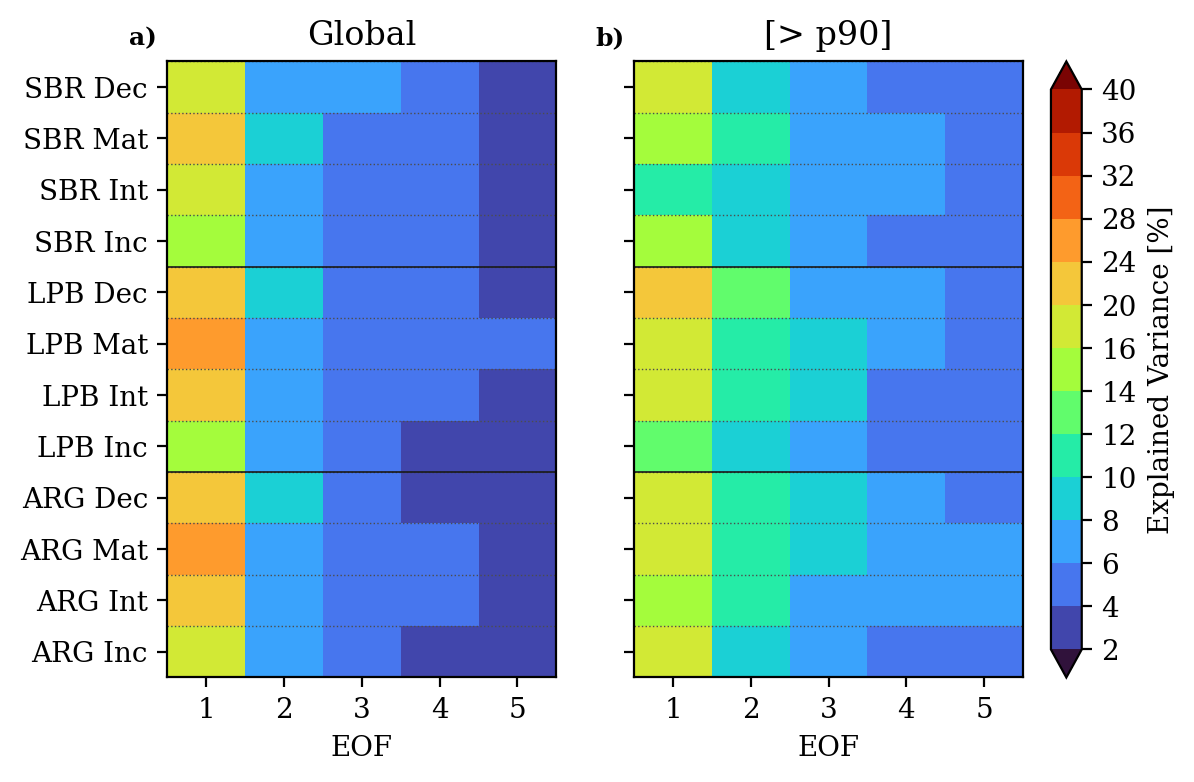
\includegraphics[width=0.8\textwidth]{images/meof/all_expvar_meof.png}
    \caption[Variância conjunta explicada pelos modos conjuntos (MEOF1--MEOF5)]{Fracionamento da variância conjunta total contida nos primeiros cinco modos espaciais multivariados (MEOF1 a MEOF5). Contrasta-se a distribuição da covariância entre o vento a 10 metros e a precipitação para a População Global (painel a) frente ao subconjunto de alta vorticidade (p90, painel b). As barras de cada linha representam as combinações de região de ciclogênese e fase evolutiva.}
    \label{fig:all_expvar_meof}
\end{figure}

\section{Evolução dos Padrões Espaciais Conjuntos (MEOF1)}
\label{sec:meof_patrones}

Os padrões espaciais do primeiro modo multivariado (MEOF1) revelam como se organiza a covariância de vento e precipitação no domínio centrado no sistema à medida que o ciclone evolui.
A análise se concentra em duas fases diagnosticamente centrais: a intensificação, onde se estabelece a configuração conjunta inicial, e a maturidade, onde a reorganização espacial entre variáveis alcança sua expressão mais marcada nos sistemas p90.

A seleção dessas duas fases, em vez das quatro que compõem o ciclo de vida (Seção~\ref{subsec:tb_fases}), obedece a duas razões.
Por um lado, a fase incipiente corresponde por definição ao surgimento inicial de uma circulação organizada, quando os sistemas ainda exibem circulações assimétricas antes de consolidar uma circulação fechada e apresentam uma variabilidade de intensidade inter-sistêmica marcadamente maior do que nas fases posteriores; essa heterogeneidade, já evidenciada na baixa e dispersa variância explicada pelo EOF1 univariado durante a incipiência (Seções~\ref{sec:var_exp_wind10} e~\ref{subsec:var_exp_tp}), reflete que a diversidade de configurações responde não apenas à região de ciclogênese mas também à falta de organização morfológica dos sistemas, o que limita a interpretabilidade física de um modo conjunto dominante.
Por outro lado, a fase de decaimento tem menor relevância prática. Os ciclones do Atlântico Sul-Ocidental deslocam sua trajetória preferencialmente em direção ao sudeste e ao oceano aberto, de modo que no decaimento a maioria dos sistemas já se encontra afastada do litoral sul-americano.
Por essas razões, a análise detalhada do MEOF1 se concentra em intensificação e maturidade, as fases onde a covariabilidade entre ambos os campos é estatisticamente mais interpretável.

\subsection{Fase de Intensificação}
\label{subsec:meof_intensificacion}

A Figura~\ref{fig:meof_intensificacion_global} apresenta o primeiro modo espacial multivariado (MEOF1) durante a intensificação para a População Global.
Cada linha corresponde a uma região de ciclogênese (SBR, LPB e ARG) e cada grupo de colunas mostra os padrões MEOF1 de precipitação (coluna esquerda) e vento a 10 metros (coluna central), junto com o índice da componente principal (PC1, coluna direita).
A escala cromática divergente quantifica as anomalias padronizadas do MEOF1, com tons vermelhos para cargas positivas e azuis para negativas no domínio centrado no sistema. A variância explicada, indicada sobre cada painel de PC1, oscila entre 18.99\% (ARG) e 22.92\% (LPB).
Esta figura é construída aplicando o MEOF sobre a matriz padronizada de anomalias conjuntas de ambas as variáveis no domínio centrado no sistema, com o fim de estabelecer o padrão de referência do desenvolvimento baroclínico padrão durante o período de intensificação do sistema na climatologia média.

\begin{figure}[htbp]
    \centering
    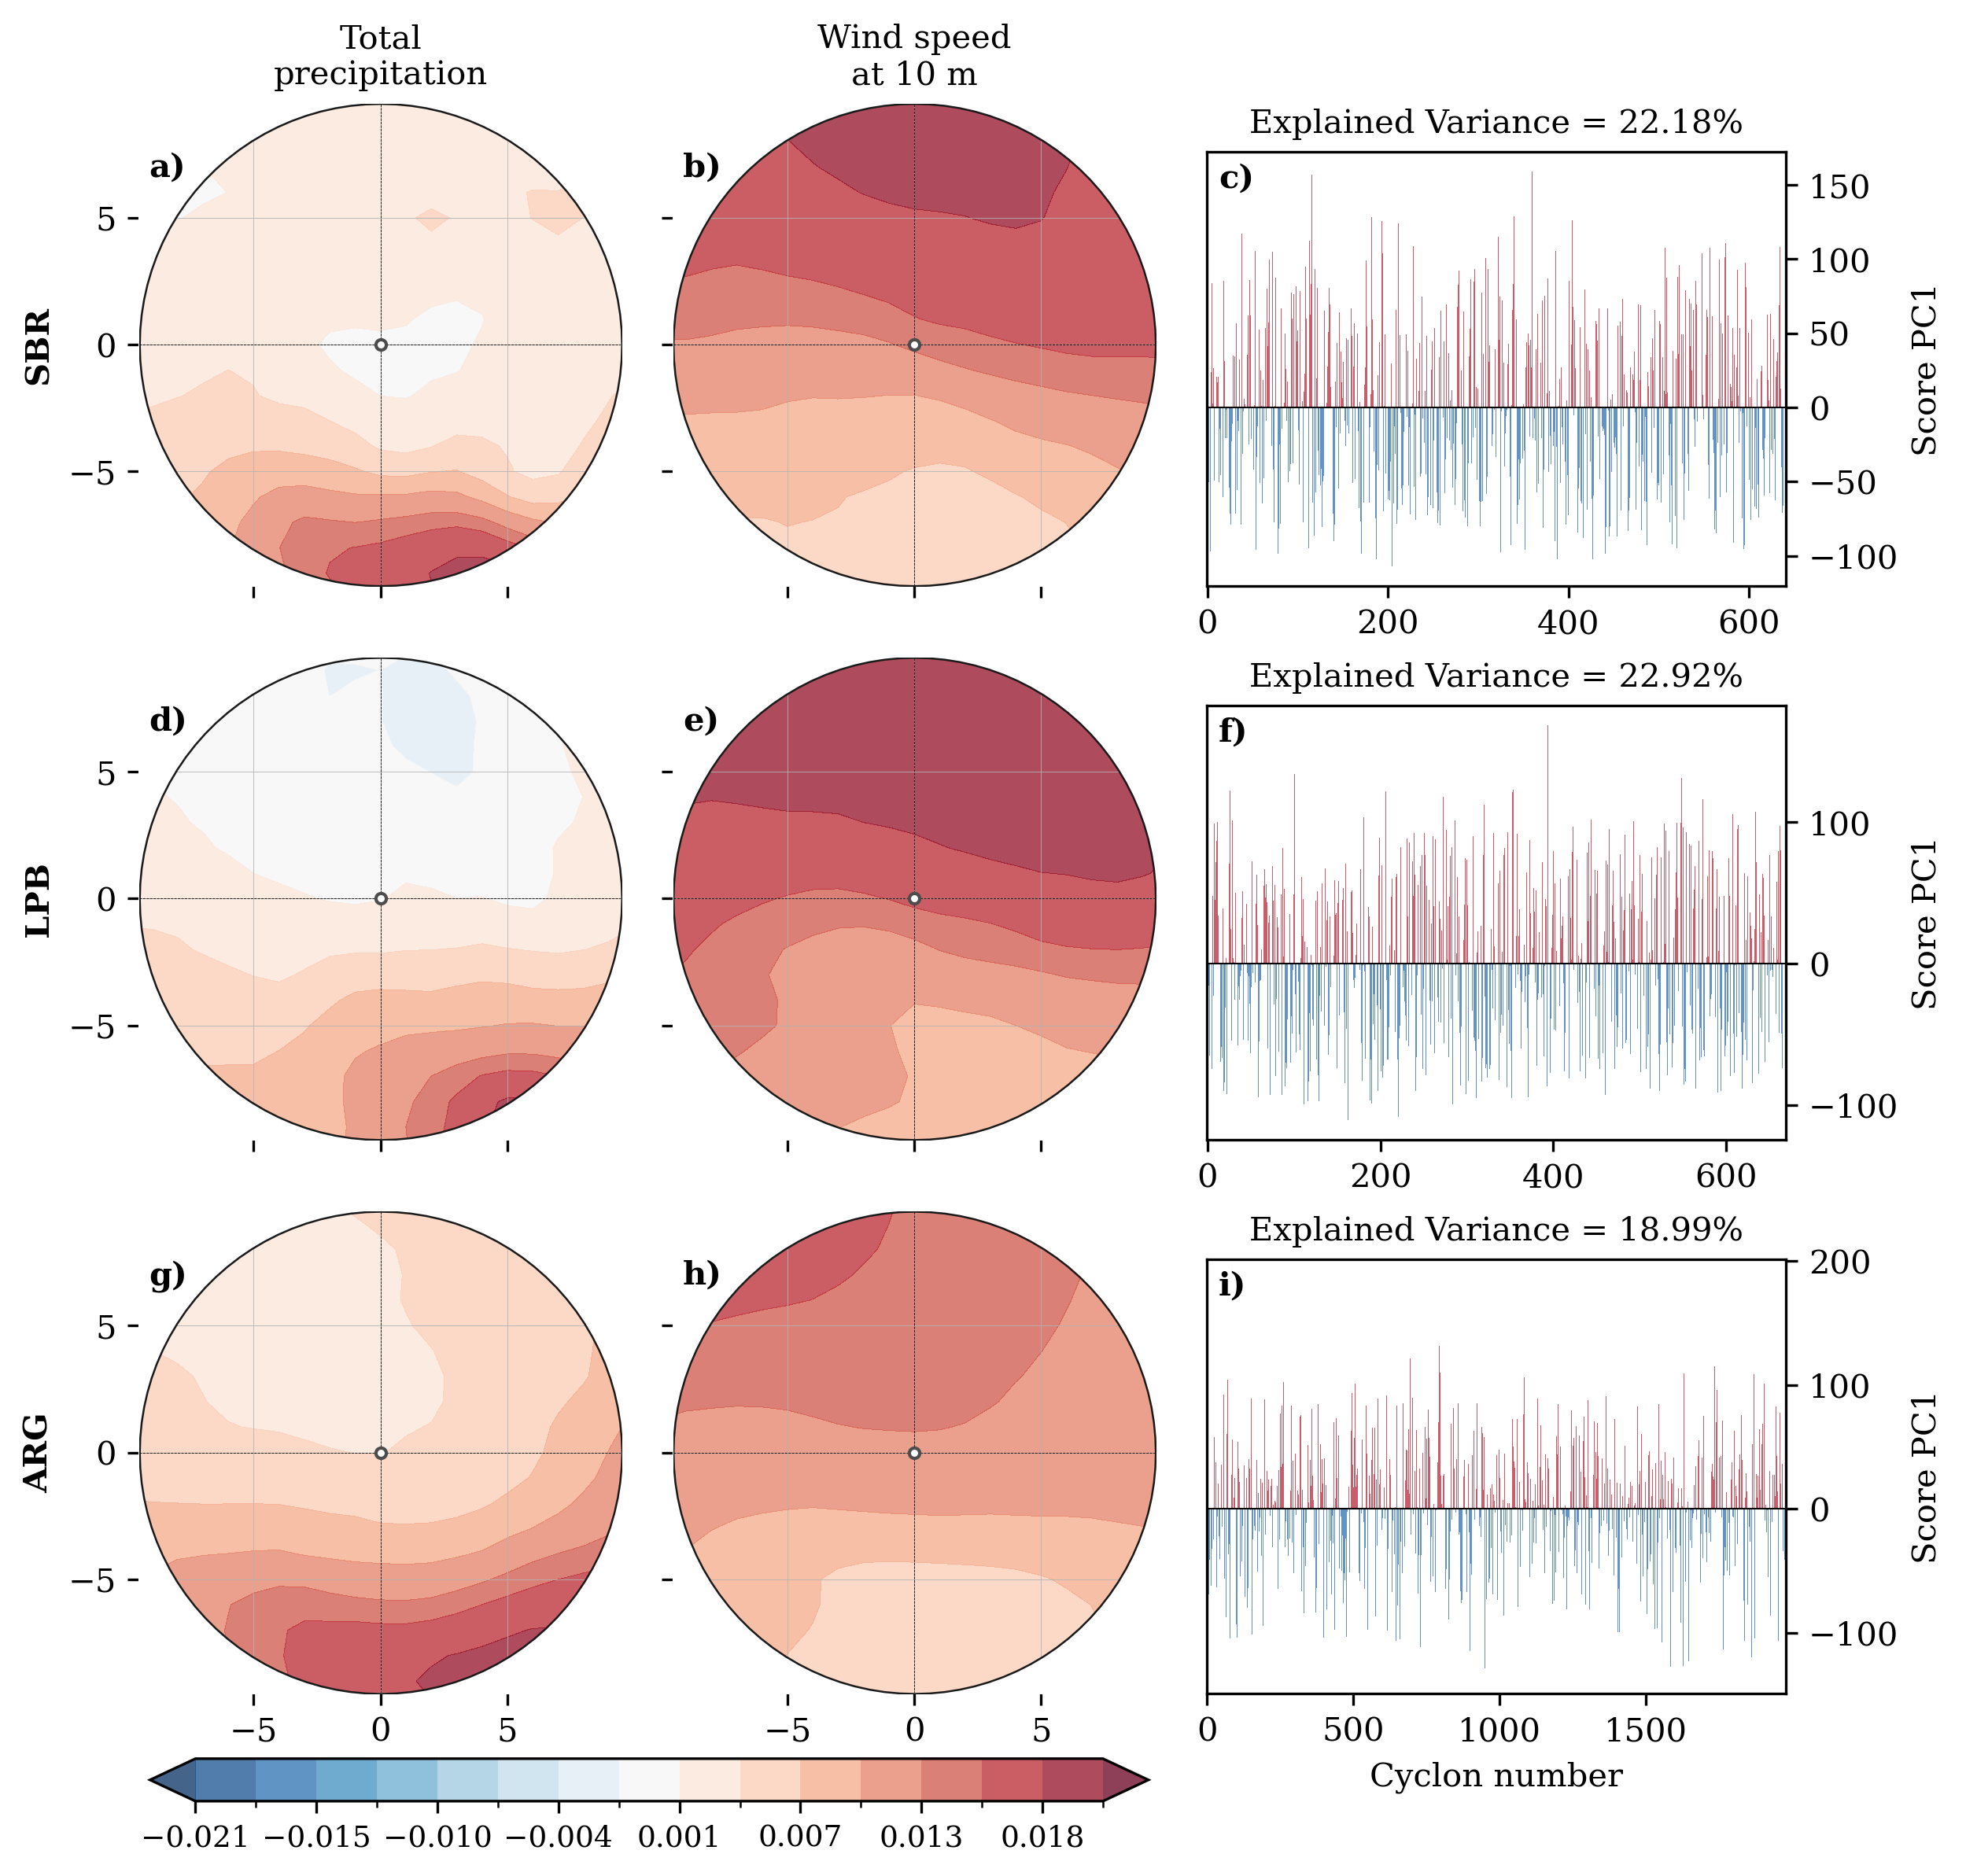
\includegraphics[width=\textwidth]{images/meof/meof1_intensification_global.png}
    \caption[MEOF1 de vento a 10 m e precipitação -- Intensificação (População Global)]{Primeiro modo espacial multivariado (MEOF1) durante a fase de intensificação para a População Global. As colunas mostram, para cada região (SBR: linhas a--c; LPB: linhas d--f; ARG: linhas g--i), os padrões MEOF1 de precipitação total (coluna esquerda), vento a 10 m (coluna central) e o índice da PC1 (coluna direita). A variância conjunta explicada é indicada sobre cada painel de PC1. A escala cromática divergente quantifica as anomalias padronizadas do MEOF1 no domínio centrado no sistema de $20^{\circ} \times 20^{\circ}$.}
    \label{fig:meof_intensificacion_global}
\end{figure}

Durante a intensificação, a População Global apresenta um padrão de covariância consistente nas três regiões, embora com matizes regionais. O campo de precipitação (painéis a, d, g) mostra anomalias positivas fracas na maior parte do domínio, com o núcleo mais definido em direção ao sul e sudeste do vórtice (até $+0.018$ em SBR e LPB); em SBR (a) e LPB (d) esse sinal se concentra em um foco compacto no quadrante sul, enquanto em ARG (g) se distribui de forma mais difusa sobre boa parte do domínio, sem um núcleo tão marcado. O campo de vento (painéis b, e, h), por sua vez, apresenta anomalias positivas muito mais intensas e estendidas, dominando a metade norte do domínio nas três regiões, particularmente em LPB (e), onde a carga positiva cobre quase todo o semicírculo norte, com valores muito altos, próximos do limite superior da escala, e decrescendo gradualmente em direção ao sul sem mudar de sinal. A correlação entre essa carga e o EOF1 univariado de cada campo (Seção~\ref{sec:discusion_meof}) mostra que, nessa fase, tanto o vento ($|r|=0.99$ a $1.00$) quanto a precipitação ($|r|=0.72$ a $0.95$) coincidem fortemente com seus próprios padrões univariados.

A Figura~\ref{fig:meof_intensificacion_p90} apresenta os mesmos padrões do MEOF1 durante a intensificação, restrita ao subconjunto de ciclones de alta vorticidade (p90).
Com disposição de painéis idêntica à figura precedente, seu propósito é documentar a primeira reorganização estrutural da covariabilidade que antecipa a diferenciação espacial completa que se consolidará na maturidade.
A variância explicada desce para valores de 11.65\% (ARG), 17.03\% (LPB) e 14.06\% (SBR), refletindo a dispersão da covariância em direção a modos secundários.

O contraste com a População Global é imediato e profundo. O campo de precipitação (painéis a, d, g) perde por completo a extensão difusa do padrão global e desenvolve uma estrutura multilobular. Em SBR (painel a) aparece um núcleo de anomalias positivas intensas e compactas ($>+0.013$) próximo do vórtice, ligeiramente deslocado para leste e para o sul ($\Delta x \approx +1^{\circ}$ a $+3^{\circ}$, $\Delta y \approx -0.5^{\circ}$ a $-2^{\circ}$), flanqueado por dois lóbulos de anomalias negativas, um a nordeste e outro ao sul, configurando já uma estrutura assimétrica de lóbulos diferenciados.
Em LPB (painel d), o padrão de precipitação mostra uma faixa de anomalias positivas com inclinação noroeste-sudeste, com o núcleo mais intenso próximo do vórtice e uma extensão secundária em direção ao noroeste, flanqueada por anomalias negativas concentradas a nordeste e, em menor medida, ao sul.
Em ARG (painel g), o núcleo positivo de precipitação é o mais intenso e compacto dos três, centrado sobre o vórtice e estendido em direção ao leste ($\Delta x \approx 0^{\circ}$ a $+5^{\circ}$, $\Delta y \approx -2^{\circ}$ a $+1^{\circ}$), com uma carga que supera o limite superior da escala ($>0.0208$) no máximo, e com anomalias negativas fracas a oeste e a nordeste.
O campo de vento (painéis b, e, h) exibe um comportamento distinto. Nas três regiões, as anomalias são negativas na maior parte do domínio, mais intensas em direção ao norte, com uma faixa de valores neutros ou levemente positivos ao sul do vórtice, onde em LPB e ARG chega até a se tornar fracamente positiva.
Esse padrão, vento que se intensifica negativamente em direção ao norte enquanto a precipitação se concentra perto do vórtice e em direção ao sul, revela já o germe da separação de quadrantes. Os máximos de precipitação e vento não covariam positivamente, mas o MEOF1 captura uma configuração de anticovariância incipiente, com o forçamento pluviométrico se concentrando onde o forçamento eólico é mais fraco. Essa mesma comparação confirma que, em p90, o vento também ancora quase por completo o modo conjunto ($|r|=0.96$ a $1.00$), exceto em ARG, onde a precipitação já contribui com covariância genuína desde essa fase ($|r|=0.92$), diferentemente de SBR e LPB ($|r|=0.08$--$0.20$), que só alcançam esse nível na maturidade (Seção~\ref{sec:discusion_meof}).

\begin{figure}[htbp]
    \centering
    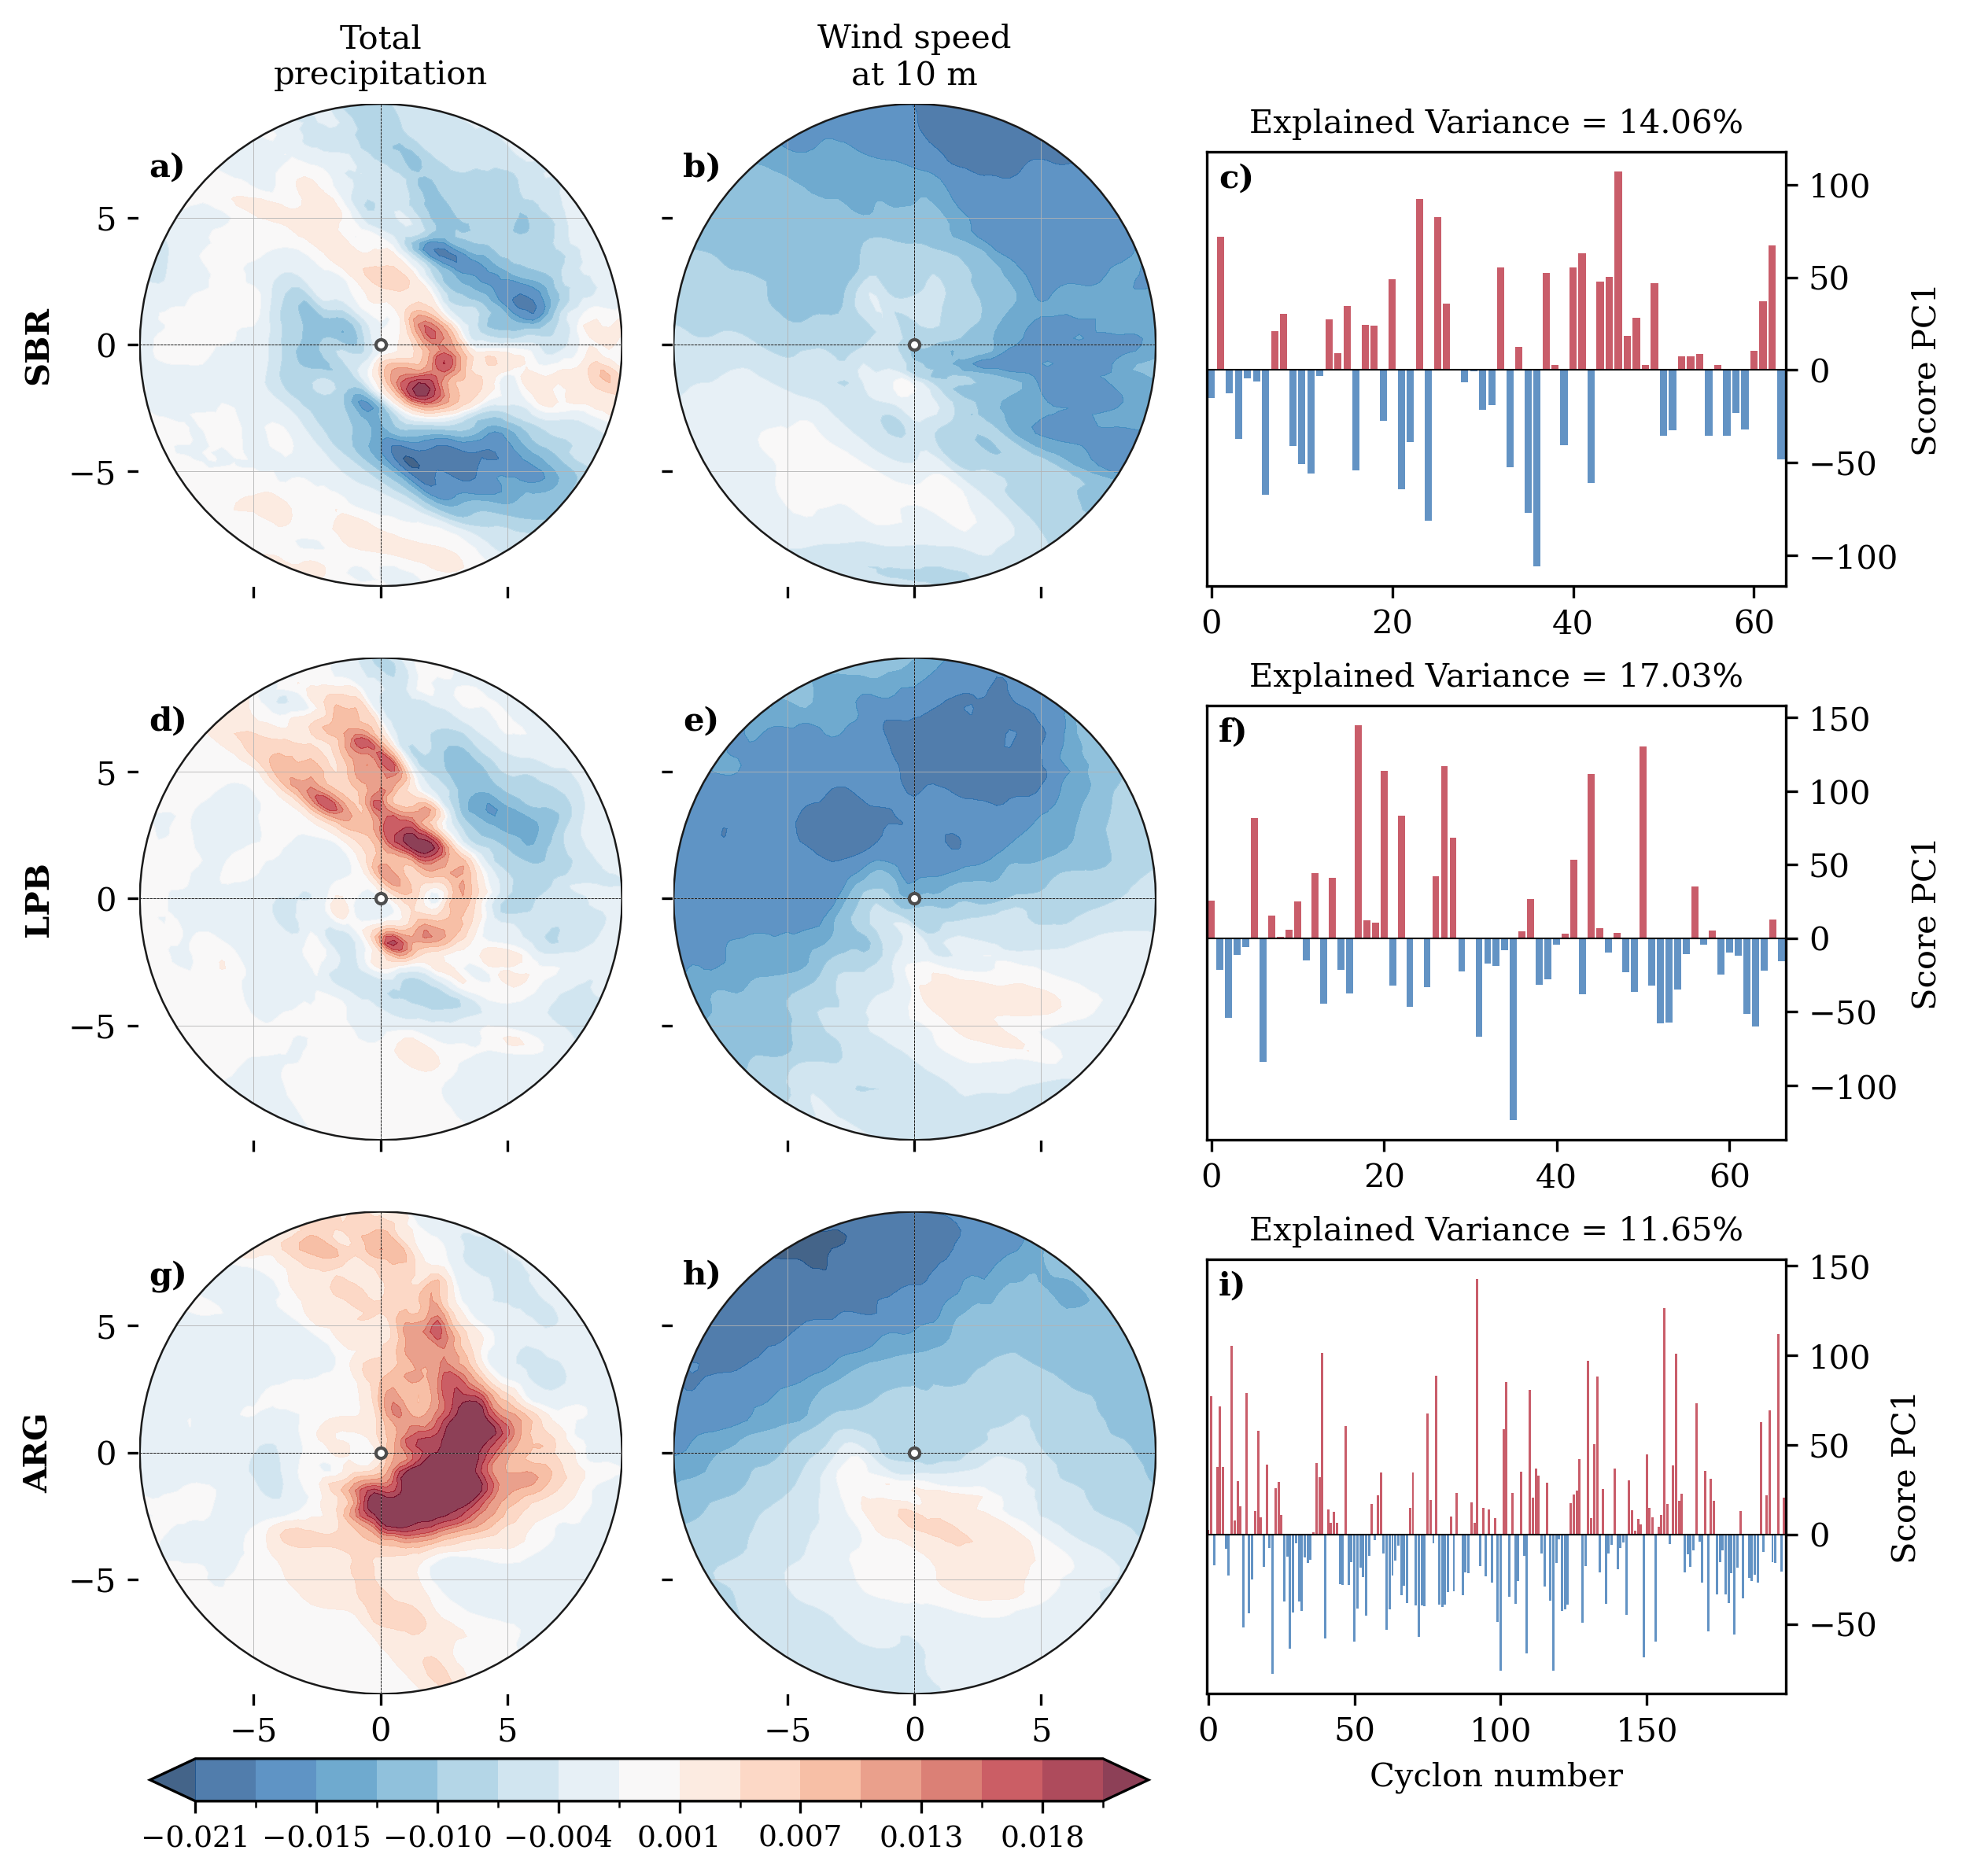
\includegraphics[width=\textwidth]{images/meof/meof1_intensification_p90.png}
    \caption[MEOF1 de vento a 10 m e precipitação -- Intensificação (p90)]{Primeiro modo espacial multivariado (MEOF1) durante a fase de intensificação para o subconjunto de ciclones de alta vorticidade (p90). O formato de painéis, a escala cromática e o domínio são idênticos à Figura~\ref{fig:meof_intensificacion_global}, permitindo quantificar a contração da covariância e a emergência da assimetria estrutural durante o desenvolvimento do sistema.}
    \label{fig:meof_intensificacion_p90}
\end{figure}

A emergência da assimetria já durante a intensificação nos sistemas p90 poderia ter uma explicação física.
Durante a intensificação baroclínica ativa, a precipitação se organiza na ascensão frontal do WCB no flanco quente-oriental do ciclone, enquanto a CCB emergente dá forma à nebulosidade da \textit{cabeça da vírgula} \citep{browning1986conceptual} e começa a envolver o núcleo do sistema.
Em ciclones ordinários, esses dois processos operam de maneira suave e parcialmente superposta, gerando a covariância difusa documentada na População Global.
Nos sistemas intensos, essa separação poderia ocorrer já durante a própria intensificação, antes de o sistema alcançar seu máximo, o que seria compatível com o fato de o MEOF1 já capturar uma covariância negativa nessa fase. A precipitação se concentra perto do vórtice e em direção ao sul enquanto o vento se intensifica em direção ao norte, antecipando a configuração oposta de quadrantes que dominará na maturidade.

\subsection{Fase de Maturidade}
\label{subsec:meof_madurez}

A Figura~\ref{fig:meof_madurez_global} expõe o MEOF1 para a fase de maturidade na População Global, correspondente ao clímax da vorticidade climatológica do sistema.
Com a mesma disposição de painéis por região (SBR, LPB, ARG) e variável (precipitação, vento, PC1), esta figura documenta a máxima organização conjunta que um ciclone ordinário alcança em seu ponto de maior intensidade.
A variância explicada oscila entre 22.31\% (ARG) e 26.59\% (LPB), os valores mais elevados do ciclo de vida na População Global.

A característica mais notável é que os padrões de precipitação (painéis a, d, g) e vento (painéis b, e, h) exibem anomalias padronizadas extensas e de grande escala, com gradientes dominantes orientados em eixos distintos do domínio. Nas três regiões, a precipitação se organiza em um gradiente oeste-leste, com um núcleo concentrado em direção ao sudoeste que se debilita e muda de sinal em direção ao leste; o vento, por sua vez, se organiza em um gradiente norte-sul, mais intenso em direção ao norte e decrescendo gradualmente em direção ao sul sem mudar de sinal.
Essa configuração, embora não constitua uma co-localização estrita, reflete a covariabilidade simples e previsível que caracteriza o ciclone ordinário maduro: ambos os campos variam suavemente em todo o domínio, sem desenvolver núcleos isolados nem transições abruptas, embora seus gradientes dominantes sejam perpendiculares entre si (oeste-leste para a precipitação, norte-sul para o vento), o que sugere que, no regime médio, cada campo responderia ao mesmo forçante sinótico de grande escala sem requerer uma geometria idêntica.
A especificidade regional reside na magnitude e forma das cargas: LPB (painéis d--f) mostra a maior variância explicada (26.59\%) e o gradiente de vento mais intenso e uniforme, que cobre praticamente toda a metade norte do domínio (painel e); SBR (painéis a--c) exibe em precipitação um núcleo concentrado no sudoeste do domínio (painel a); ARG (painéis g--i) mostra a menor variância explicada (22.31\%) e padrões mais difusos, refletindo a maior variabilidade estrutural dos sistemas dessa região.

\begin{figure}[htbp]
    \centering
    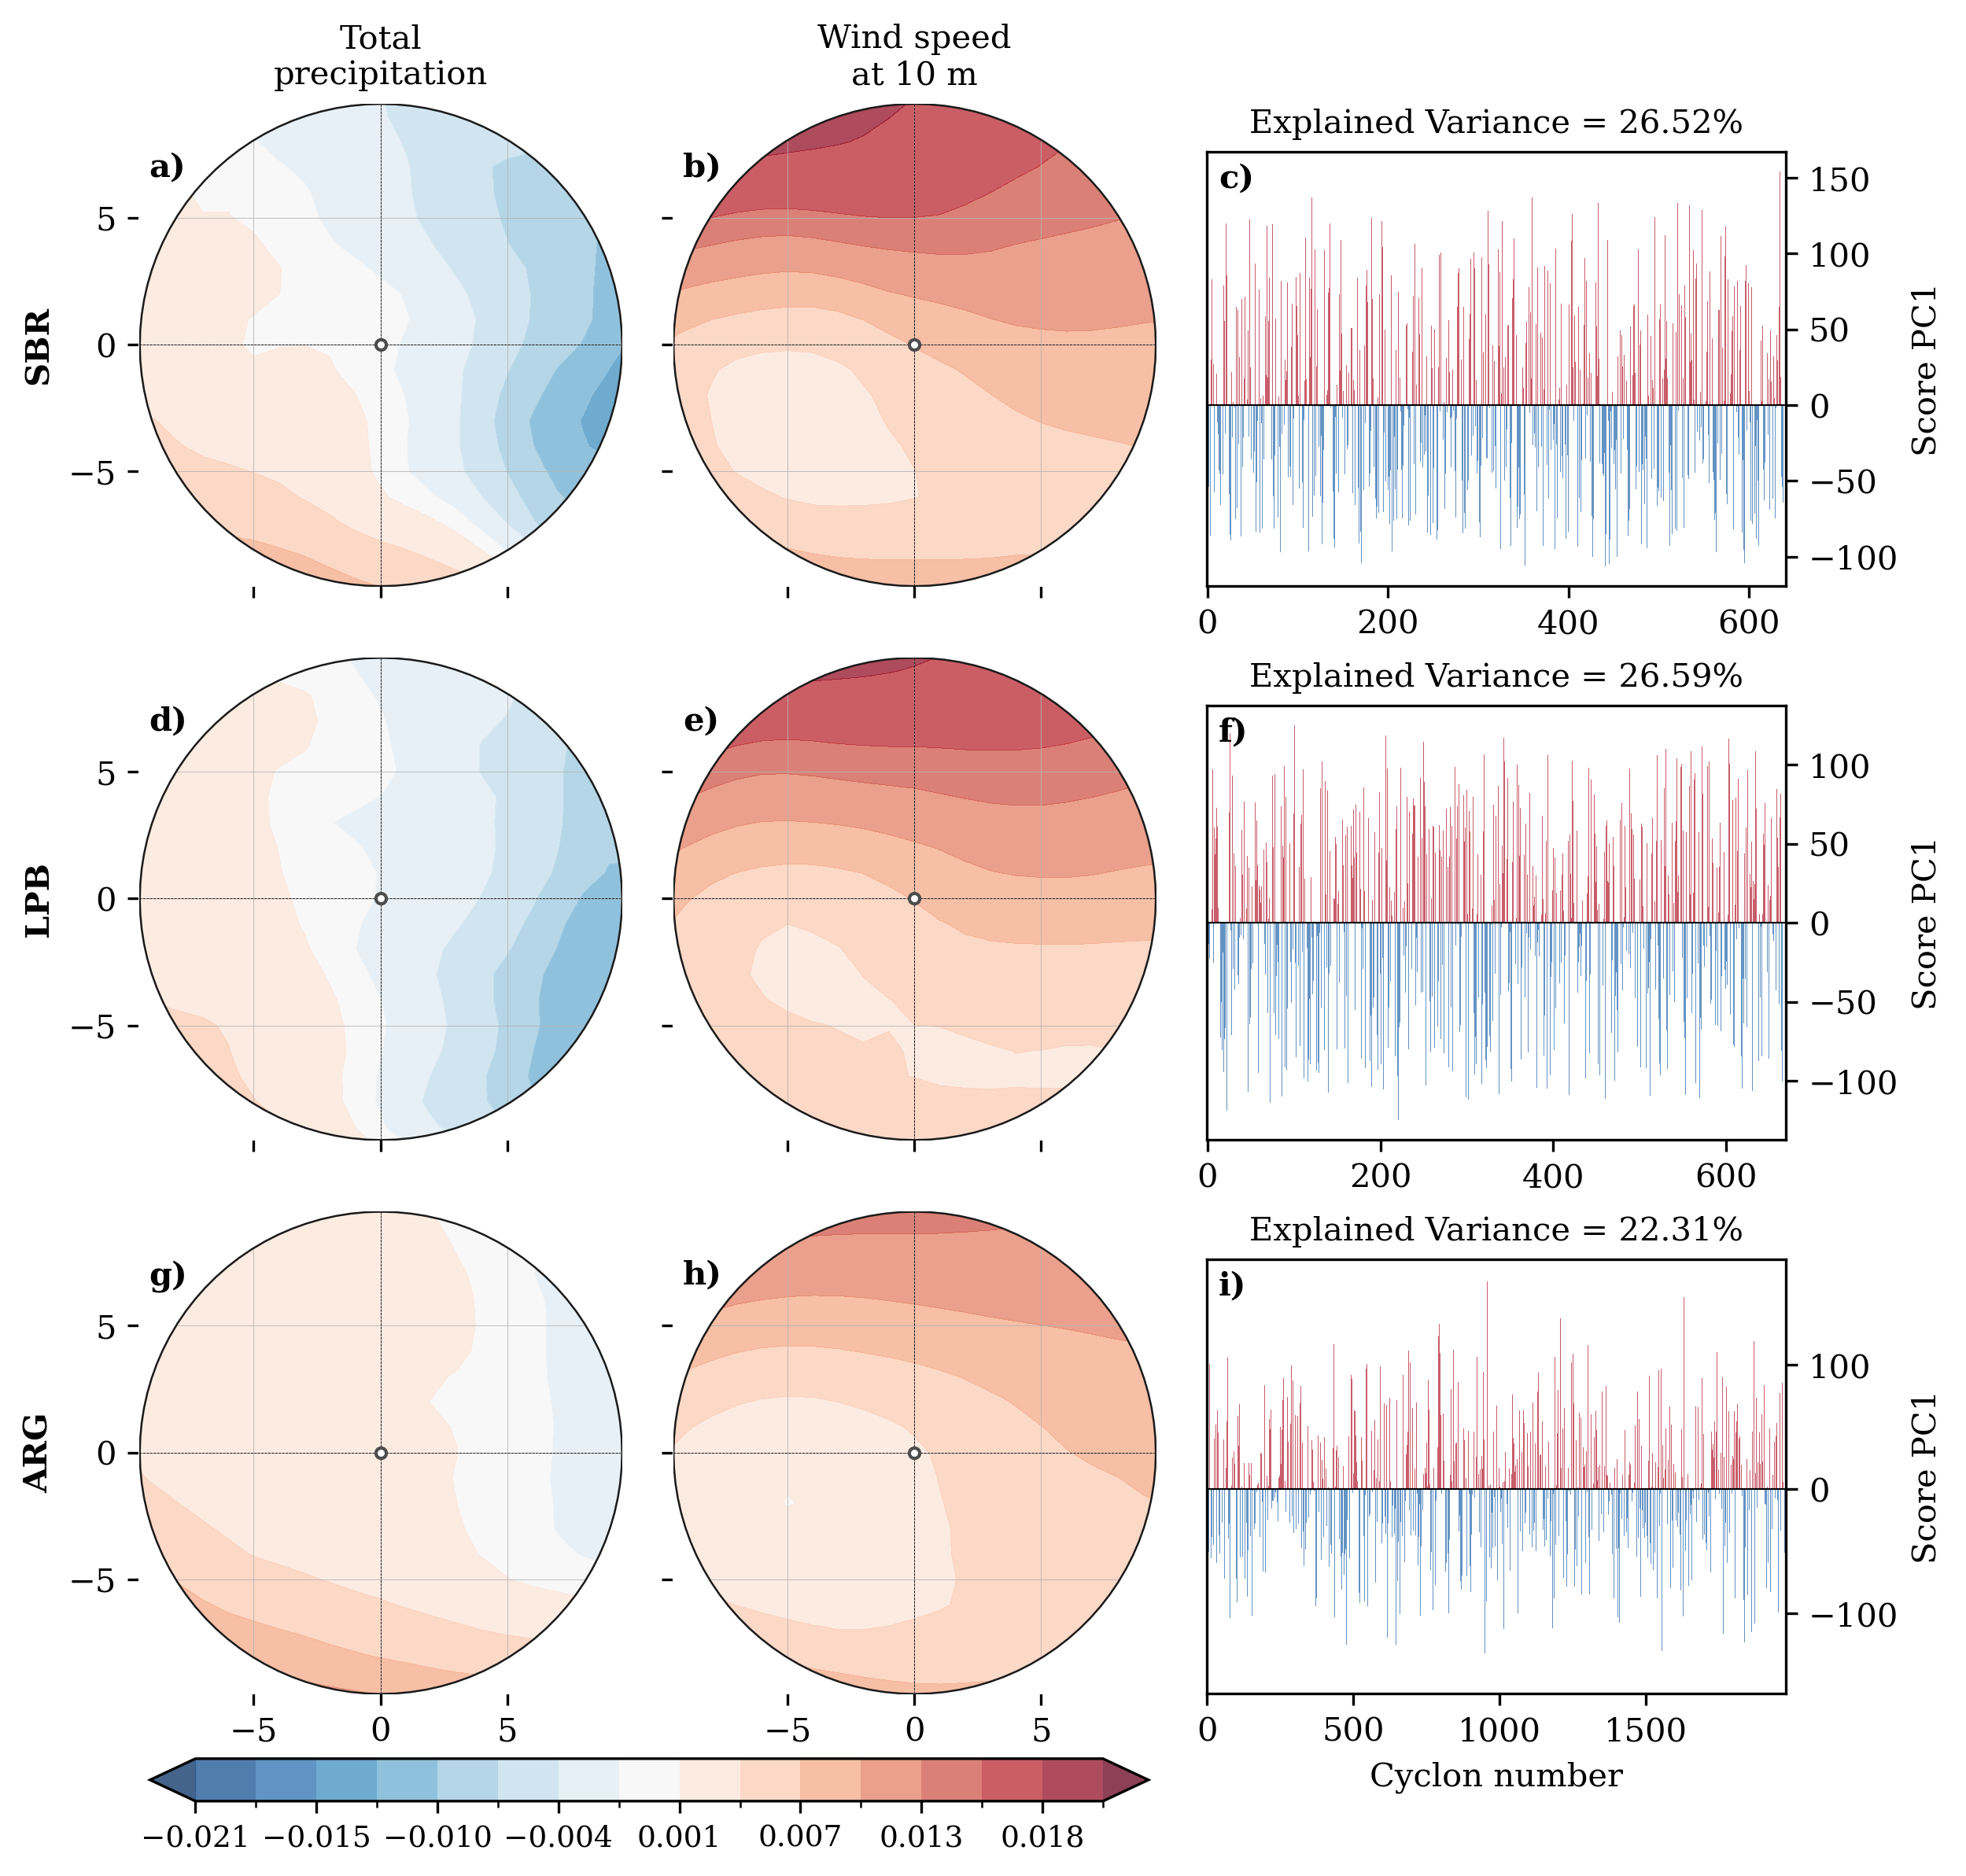
\includegraphics[width=\textwidth]{images/meof/meof1_mature_global.png}
    \caption[MEOF1 de vento a 10 m e precipitação -- Maturidade (População Global)]{Primeiro modo espacial multivariado (MEOF1) correspondente à fase de maturidade para a População Global. A disposição de painéis é idêntica às figuras precedentes. Documenta-se o padrão de covariabilidade de grande escala que caracteriza o ciclone ordinário em sua máxima intensidade, estabelecendo a linha de base em relação à qual se avalia a transformação estrutural do subconjunto de alta vorticidade.}
    \label{fig:meof_madurez_global}
\end{figure}

A Figura~\ref{fig:meof_madurez_p90} apresenta a matriz de cargas espaciais do MEOF1 para o subconjunto de alta vorticidade (p90) na fase de maturidade.

Com disposição idêntica de painéis, esta figura constitui o núcleo do capítulo. Seu propósito é mostrar a reorganização espacial entre os campos de precipitação e vento nos sistemas p90 do Atlântico Sul. O fato de cada componente univariada ser significativa separadamente (Seções~\ref{subsec:res_significancia_madurez} e~\ref{subsec:significancia_tp}) não garante que o modo conjunto também o seja. Não se conta com uma reamostragem Bootstrap-t multivariada independente para esta figura; essa limitação é retomada mais adiante (Seção~\ref{sec:discusion_meof}), ao mostrar que o modo conjunto às vezes reflete majoritariamente um único campo.
A variância conjunta explicada cai para 15.41\% (ARG), 16.42\% (LPB) e 19.02\% (SBR), muito abaixo dos valores da População Global na mesma fase, e também abaixo do EOF1 univariado de cada campo separadamente em p90-maturidade (vento: 25.4--37.6\%, Seção~\ref{sec:var_exp_wind10}; precipitação: 16--21.4\%, Seção~\ref{subsec:var_exp_tp}). O modo conjunto não é apenas menos dominante do que na População Global, mas menor do que qualquer um dos dois campos separadamente, consistente com o fato de ambos os campos se organizarem em setores geometricamente distintos do domínio (Figura~\ref{fig:meof_madurez_p90}), de modo que um único autovetor não pode capturar ambos os padrões com a mesma eficiência com que cada EOF univariado captura o seu. Essa separação, não a variância explicada, é o sinal que o MEOF permite identificar, e não uma limitação do método. Essa mesma ordem regional (SBR $>$ LPB $>$ ARG) já apareceu na concentração de magnitude e na densidade espacial dos máximos de vento (Seção~\ref{sec:kde_espacial_p90}), a terceira vez que se repete com um método distinto, agora em nível multivariado.

O contraste com a figura precedente é o mais marcado do capítulo.
O campo de precipitação (painéis a, d, g) exibe nas três regiões uma estrutura em arco compacta de anomalias positivas concentrada no quadrante sudeste e sul do domínio, com cargas que alcançam $+0.018$ em SBR (painel a) e $+0.015$ em LPB (painel d), indicando que o modo captura um padrão de precipitação localizado e recorrente nesse setor específico. Em SBR, o arco de precipitação (painel a) parte do sul e se estende em direção ao leste e nordeste.
Em LPB (painel d), a faixa é mais larga e se estende do quadrante sul até o leste, com o pico de carga deslocado em direção ao sudeste ($\Delta x \approx +3^{\circ}$, $\Delta y \approx -3^{\circ}$). Em ARG (painel g), o padrão de precipitação é o mais difuso dos três, com cargas positivas distribuídas no sudeste-sul mas com gradientes mais suaves.
O campo de vento (painéis b, e, h) apresenta uma configuração oposta. As anomalias positivas se concentram em um núcleo compacto a oeste do centro, aproximadamente na sua mesma latitude, com cargas que alcançam $+0.013$ em SBR (painel b) e $+0.010$ em LPB (painel e).
Esse núcleo de vento a oeste e o arco de precipitação a sudeste não apenas não compartilham setor, mas no domínio centrado no sistema se localizam em lados opostos em relação ao centro do vórtice (0,0).

\begin{figure}[htbp]
    \centering
    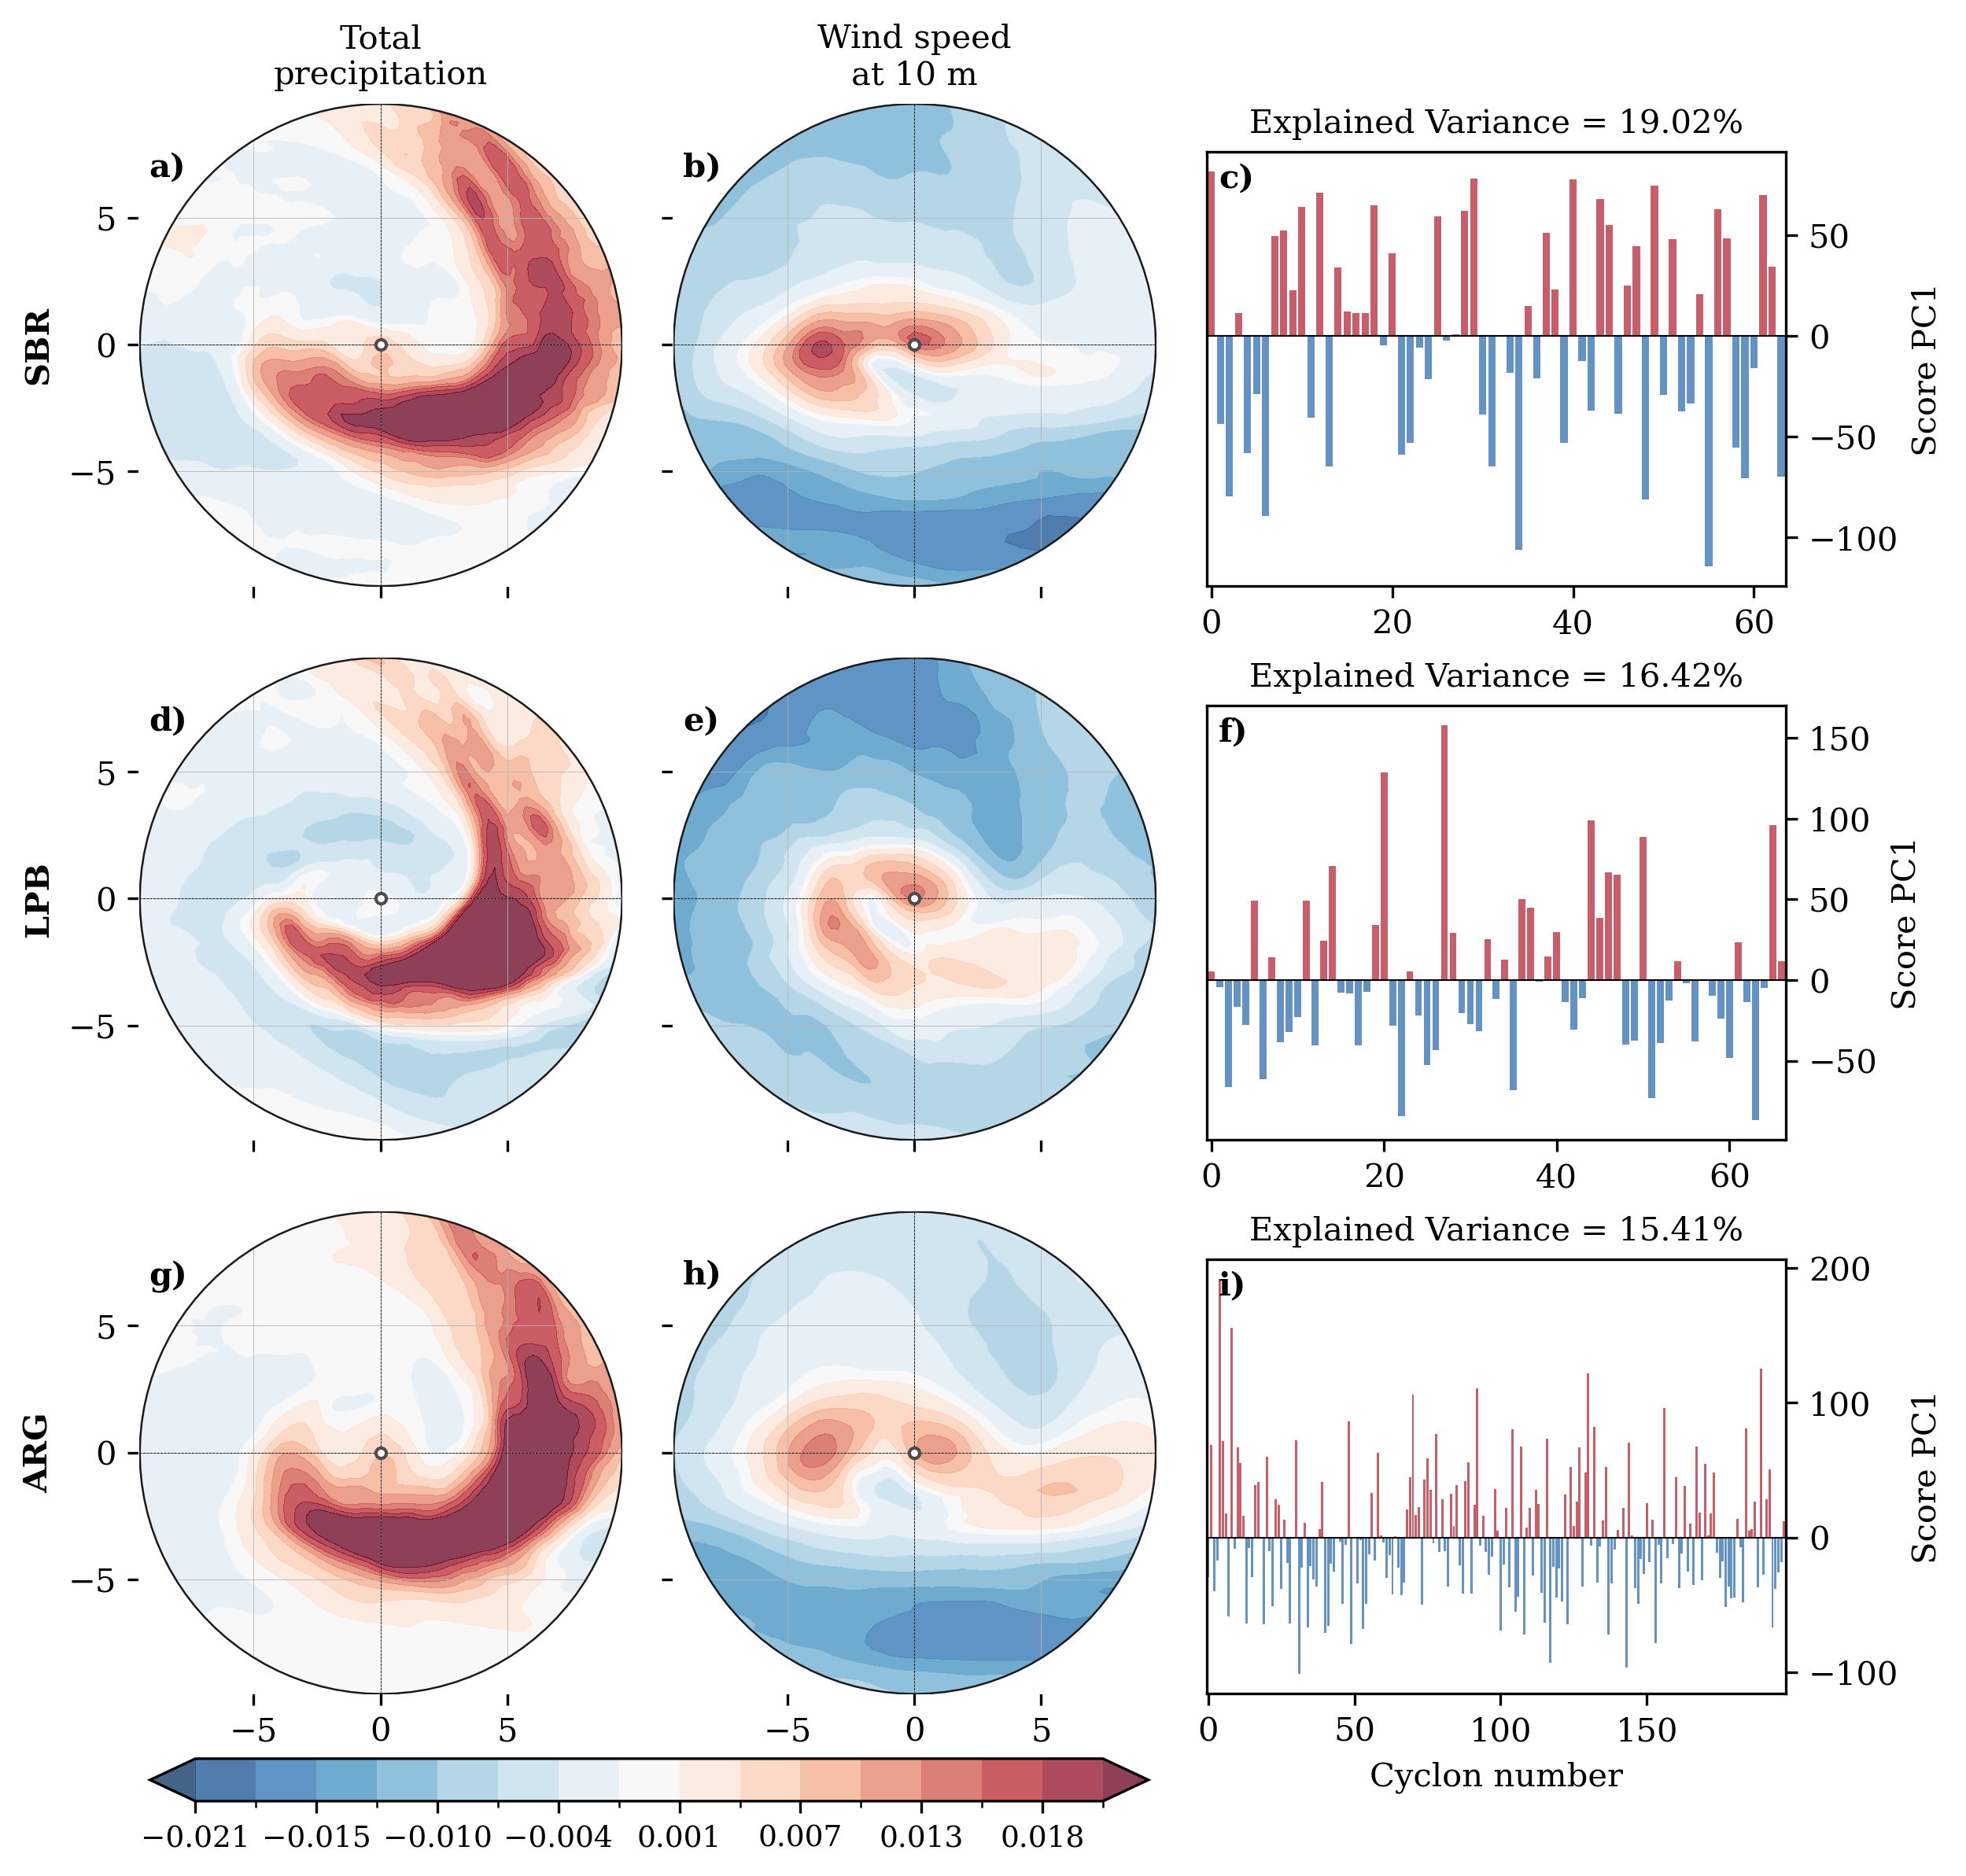
\includegraphics[width=\textwidth]{images/meof/meof1_mature_p90.png}
    \caption[MEOF1 de vento a 10 m e precipitação -- Maturidade (p90)]{Primeiro modo espacial multivariado (MEOF1) correspondente à fase de maturidade para o subconjunto de ciclones de alta vorticidade (p90). A disposição de painéis, a escala cromática e o domínio são idênticos às figuras precedentes.
Evidencia-se a reorganização espacial entre a banda de precipitação periférica no quadrante sudeste e o núcleo de vento a oeste do vórtice, a separação em quadrantes opostos que caracteriza os sistemas p90 do Atlântico Sul nessa fase.}
    \label{fig:meof_madurez_p90}
\end{figure}

A configuração de setores opostos documentada no MEOF1 de maturidade do subconjunto p90 é a evidência multivariada que integra e é coerente com os resultados dos capítulos precedentes.
O arco de precipitação sudeste capturado pelo MEOF1 corresponde à estrutura em arco periférica cuja assinatura PDFe foi documentada na Seção~\ref{subsec:kde_tp_p90} e cuja concentração de variância foi quantificada no EOF1 univariado (Seção~\ref{subsec:var_exp_tp}).
O núcleo de vento a oeste do MEOF1 coincide parcialmente com a concentração espacial identificada no PDFe de vento p90 (Seção~\ref{sec:kde_espacial_p90}) e com a estrutura compacta do EOF1 univariado de vento (Seção~\ref{subsec:eof1_wind10_p90}); embora ambos coincidam no setor ocidental, o núcleo de alta densidade da análise univariada se localiza no quadrante noroeste ($\Delta y \approx +2^{\circ}$ a $+3^{\circ}$), enquanto no MEOF1 o núcleo se localiza praticamente na mesma latitude do vórtice ($\Delta y \approx 0^{\circ}$), um deslocamento em direção ao sul sem causa determinada, que poderia se dever tanto à covariância com a precipitação quanto a um artefato da decomposição conjunta (Seção~\ref{sec:discusion_meof}). A novidade que o MEOF traz é que, ao decompor a covariância conjunta, mostra que a separação entre ambos os campos não é a justaposição acidental de dois padrões independentes, mas uma configuração geométrica estruturalmente coerente. O MEOF1 a captura como um único modo multivariado, o que indica que a precipitação ao sudeste e o vento a oeste covariam nos mesmos eventos, constituindo o padrão conjunto dominante da estrutura no Atlântico Sul.

A interpretação física dessa reorganização espacial poderia estar relacionada ao modelo de ciclone ocluso de Shapiro-Keyser. Em um ciclone do Hemisfério Norte com seclusão quente, \citet{shapiro1999bridge} documenta subsidência a oeste do centro, o que seria compatível com o fato de o núcleo de vento a oeste capturado pelo MEOF1 coincidir com ar mais seco e menos convectivo do que o setor sudeste, onde se concentra a precipitação. Em ciclones do Hemisfério Norte documentam-se ainda ventos extremos associados ao \textit{sting jet} e ao jato da cinta transportadora fria (CCB), situado abaixo e atrás dele \citep{clark2005sting, clark2018sting}, duas estruturas difíceis de distinguir em superfície por sua proximidade no espaço e no tempo \citep{eisenstein2023identification}; pela inversão da circulação entre hemisférios, esse setor corresponderia ao quadrante ocidental no Hemisfério Sul, coerente com a localização do núcleo de vento do MEOF1. Essa interpretação se apoia em estudos do Hemisfério Norte e em um caso único (Shapiro 1999), sem verificação direta para o Atlântico Sul.

\section{Coerência entre os Modos de Vento e Precipitação}
\label{sec:meof_coherencia}

Para confirmar se a reorganização espacial observada nos padrões do MEOF1 se traduz também em uma relação entre os dois campos em nível de eventos individuais, analisa-se a correlação entre as Componentes Principais univariadas de cada campo ($\text{PC1}^{\text{precip}}$ e $\text{PC1}^{\text{vento}}$), seguindo a metodologia descrita na Seção~\ref{subsec:analisis_pc}. Os resultados são apresentados na Tabela~\ref{tab:meof_coherencia}, que quantifica a evolução dessa relação ao longo do ciclo de vida para ambas as populações, com o fim de determinar se a separação espacial dos campos implica também que os ciclones que mais projetam sobre um padrão tendem a projetar menos sobre o outro.

\begin{table}[htbp]
\centering
\caption[Coerência entre os modos de precipitação e vento a 10m (Global e p90)]{Correlação de Spearman em valor absoluto ($|r|$) entre a PC1 de precipitação e a PC1 do vento a 10 metros, e seu valor de significância (\textit{p-valor}), para a População Global e o subconjunto extremo (p90). Reporta-se o valor absoluto porque cada PC1 provém de uma decomposição EOF univariada independente, com sua própria convenção de sinal arbitrária (Seção~\ref{subsec:analisis_pc}). Os valores em negrito indicam correlações estatisticamente significativas ($p < 0.05$).}
\label{tab:meof_coherencia}
\begin{tabular*}{\textwidth}{@{\extracolsep{\fill}}llrrrr}
\hline
\textbf{Região} & \textbf{Fase} & \multicolumn{2}{c}{\textbf{População Global}} & \multicolumn{2}{c}{\textbf{Subconjunto p90}} \\
\cline{3-4} \cline{5-6}
 & & \textbf{$|r|$} & \textbf{p-valor} & \textbf{$|r|$} & \textbf{p-valor} \\
\hline
\textbf{SBR} & Incipiente & \textbf{0.31} & $<$ 0.001 & \textbf{0.32} & 0.009 \\
 & Intensificação & \textbf{0.39} & $<$ 0.001 & 0.01 & 0.946 \\
 & Maturidade & \textbf{0.19} & $<$ 0.001 & \textbf{0.45} & $<$ 0.001 \\
 & Decaimento & \textbf{0.19} & $<$ 0.001 & 0.07 & 0.571 \\
\hline
\textbf{LPB} & Incipiente & \textbf{0.25} & $<$ 0.001 & 0.13 & 0.285 \\
 & Intensificação & \textbf{0.35} & $<$ 0.001 & 0.06 & 0.648 \\
 & Maturidade & \textbf{0.08} & 0.029 & \textbf{0.37} & 0.002 \\
 & Decaimento & \textbf{0.08} & 0.032 & 0.12 & 0.314 \\
\hline
\textbf{ARG} & Incipiente & \textbf{0.18} & $<$ 0.001 & 0.03 & 0.647 \\
 & Intensificação & \textbf{0.47} & $<$ 0.001 & 0.08 & 0.236 \\
 & Maturidade & \textbf{0.44} & $<$ 0.001 & \textbf{0.31} & $<$ 0.001 \\
 & Decaimento & \textbf{0.23} & $<$ 0.001 & \textbf{0.35} & $<$ 0.001 \\
\hline
\end{tabular*}
\end{table}


Na População Global, as correlações entre $\text{PC1}^{\text{precip}}$ e $\text{PC1}^{\text{vento}}$ são significativas durante as fases iniciais nas três regiões (Tabela~\ref{tab:meof_coherencia}), com magnitudes que oscilam entre $|r|=0.18$ e $0.47$. Em SBR e LPB, a correlação perde magnitude até a maturidade e o decaimento, embora se mantenha significativa ($|r|=0.19$ e $0.08$, respectivamente). Em ARG, por sua vez, a correlação se mantém significativa durante todo o ciclo de vida, alcançando seu máximo na intensificação ($|r|=0.47$) e mantendo-se quase igualmente forte na maturidade ($|r|=0.44$) antes de se atenuar no decaimento ($|r|=0.23$).

A correlação entre PC1 de precipitação e PC1 de vento durante a maturidade em p90 é significativa e de magnitude moderada nas três regiões ($|r| = 0.45$ em SBR, $0.37$ em LPB e $0.31$ em ARG). Esses dois índices provêm de decomposições EOF univariadas independentes (precipitação, Capítulo~\ref{cap:resultados_tp}; vento, Capítulo~\ref{cap:resultados_wind10}), cada uma com sua própria convenção de sinal arbitrária. Nessa fase e população, o núcleo positivo do EOF1 de precipitação se localiza a leste-sudeste e o do EOF1 de vento a oeste nas três regiões (Seções~\ref{subsec:eof1_tp_p90} e~\ref{subsec:eof1_wind10_p90}); com essa referência espacial verificada, o sinal observado indica que os ciclones com maior projeção sobre o núcleo sudeste de precipitação tendem a ter uma projeção menor ou nula sobre o núcleo ocidental de vento, e vice-versa, consistente com a separação em quadrantes opostos documentada no MEOF para essa mesma fase e população. No decaimento, SBR e LPB perdem significância ($|r|=0.07$ e $0.12$), enquanto ARG mantém uma correlação significativa de magnitude semelhante à da maturidade ($|r|=0.35$); essa persistência em magnitude é consistente com a maior dominância de seu EOF1 já apontada (Seção~\ref{subsec:pc1_global_tp}).

\section{Discussão}
\label{sec:discusion_meof}
% ==============================================================================

Os resultados da análise MEOF revelam uma transição qualitativa na relação espacial entre vento e precipitação que não é detectável mediante a análise univariada de cada variável separadamente.
Nos ciclones da População Global, o MEOF1 captura um padrão de covariância simples e extenso onde vento e precipitação permanecem majoritariamente positivos em todo o domínio centrado no sistema, sem núcleos isolados nem mudanças de sinal abruptas, com uma variância conjunta explicada entre 14.8\% e 26.6\%. Essa configuração reflete o desenvolvimento baroclínico clássico do modelo norueguês de frentes \citep{bjerknes1922life}, sistematizado posteriormente no marco do WCB como estrutura termodinâmica única que organiza a ascensão úmida (precipitação) e o fluxo de baixo nível (vento) no setor quente do ciclone \citep{browning1986conceptual}.
A suavidade e a extensão compartilhada das cargas MEOF1 de ambas as variáveis, embora orientadas em eixos distintos (oeste-leste em precipitação, norte-sul em vento), é a expressão quantitativa de que, no regime médio, os dois campos são manifestações do mesmo forçante sinótico e operam como uma estrutura dinâmica comum, sem que isso implique uma co-localização geométrica estrita.

A transição para o subconjunto p90 introduz uma mudança de regime que não pode ser atribuída a uma mera amplificação do padrão global.
A queda da variância conjunta explicada (de ${\sim}$26.6\% para ${\sim}$11.65--23.47\%) e a emergência de padrões de anticovariância entre precipitação e vento já durante a intensificação indicam que os ciclones p90 desenvolvem uma arquitetura multivariada diferente desde antes de alcançar sua maturidade.
Esse resultado é coerente com a classificação de \citet{corner2025classification}, que mostram mediante análise de componentes principais dispersas que as métricas dinâmicas dos ciclones mais intensos do Atlântico Norte e Europa não escalam linearmente com as métricas de impacto (precipitação, pegada de vento, severidade), mas exibem uma multidimensionalidade que requer várias medidas independentes para ser caracterizada.
No Hemisfério Sul, o MEOF fornece evidência equivalente mas no espaço da covariância espacial conjunta. O modo dominante já não captura um padrão simples e extenso, mas a geometria de separação entre os dois campos dinâmicos.

Um pressuposto central do MEOF é que o modo dominante reflete covariabilidade genuína entre ambos os campos, não a estrutura individual de um deles. \citet{bretherton1992intercomparison} advertem que essa abordagem pode se enviesar em direção ao EOF dominante de um único campo quando a razão sinal-ruído é baixa ou o tamanho amostral é reduzido (Seção~\ref{subsec:tb_eof}). Para avaliar esse risco, calculou-se a correlação espacial entre a carga de cada campo dentro do MEOF1 e o padrão de seu próprio EOF1 univariado, na mesma região, fase e população (Tabela~\ref{tab:meof_bias_check}, e Tabela~\ref{tab:meof_bias_check_completa} do Apêndice~\ref{apendice:meof_bias} para as quatro fases; o sinal de cada EOF é uma convenção independente e arbitrária entre decomposições distintas, por isso se reporta o valor absoluto).

\begin{table}[htbp]
\centering
\caption[Correlação espacial entre o MEOF1 e os EOF1 univariados (Global e p90)]{Correlação espacial (valor absoluto, $|r|$) entre a carga de cada campo dentro do MEOF1 e o padrão de seu próprio EOF1 univariado (vento a 10 m, Seção~\ref{sec:var_exp_wind10}; precipitação, Seção~\ref{subsec:var_exp_tp}), para a População Global e o subconjunto p90, nas fases incipiente e maturidade. As fases de intensificação e decaimento são apresentadas na Tabela~\ref{tab:meof_bias_check_completa} (Apêndice~\ref{apendice:meof_bias}).}
\label{tab:meof_bias_check}
\begin{tabular*}{\textwidth}{@{\extracolsep{\fill}}llrrrr}
\hline
\textbf{Região} & \textbf{Fase} & \multicolumn{2}{c}{\textbf{População Global}} & \multicolumn{2}{c}{\textbf{Subconjunto p90}} \\
\cline{3-4} \cline{5-6}
 & & \textbf{$|r|$ vento} & \textbf{$|r|$ precip.} & \textbf{$|r|$ vento} & \textbf{$|r|$ precip.} \\
\hline
\textbf{SBR} & Incipiente & 0.99 & 0.83 & 0.99 & 0.74 \\
 & Maturidade & 1.00 & 0.55 & 0.99 & 0.94 \\
\hline
\textbf{LPB} & Incipiente & 0.99 & 0.94 & 0.99 & 0.25 \\
 & Maturidade & 1.00 & 0.33 & 0.94 & 0.97 \\
\hline
\textbf{ARG} & Incipiente & 1.00 & 0.56 & 1.00 & 0.49 \\
 & Maturidade & 0.99 & 0.79 & 0.94 & 0.97 \\
\hline
\end{tabular*}
\end{table}


A carga de vento do MEOF1 coincide quase por completo com seu EOF1 univariado em praticamente todas as combinações de região, fase e população ($|r|>0.94$), tanto na População Global quanto em p90, exceto no decaimento de p90 para SBR ($|r|=0.26$) e LPB ($|r|=0.71$), onde o vento se debilita notavelmente. A carga de precipitação é muito mais variável. Na População Global flutua entre $|r|=0.33$ e $0.95$ sem uma tendência clara por fase ou região. Em p90, por sua vez, o padrão é mais definido: fraco em incipiente e intensificação em SBR e LPB ($|r|=0.08$ a $0.25$), e forte e consistente desde a maturidade nas três regiões ($|r|=0.85$ a $1.00$); ARG se mantém alto desde a intensificação ($|r|\geq0.92$). Isso indica que o vento ancora o MEOF1 em quase todas as combinações, e que a precipitação contribui com covariância genuína de forma mais sistemática em p90 a partir da maturidade do que na População Global, onde sua contribuição é mais errática. Essa leitura é consistente com a interpretação de viés em direção ao vento como regra geral, embora não se possa descartar que a correlação mais baixa de precipitação em p90-incipiente reflita também a menor variância explicada pelo próprio EOF1 univariado de precipitação nessa fase (13.8--15.3\% frente a 16.0--21.4\% na maturidade; Seção~\ref{subsec:var_exp_tp}).

A configuração de quadrantes opostos documentada no MEOF1 de maturidade do subconjunto p90 permite, além disso, estabelecer uma hierarquia física dos processos envolvidos.
A estrutura em arco de precipitação no quadrante sudeste capturada pelo MEOF1 se localiza em uma posição mais próxima da do WCB do que da do quadrante ocluso que \citet{martin1999forcing} descreve para a corrente do trowal (Seção~\ref{subsec:kde_tp_p90}); a convecção embutida no WCB, documentada por \citet{oertel2021warm} em um ciclone do Atlântico Norte, poderia sustentar a intensidade pluviométrica localizada nesse setor.
A organização do vento no setor ocidental é consistente com a caracterização da CCB como principal motor da circulação de baixo nível na fase de oclusão, que \citet{martinez2014cold} documenta observacionalmente e que \citet{eisenstein2023identification} confirma em climatologias europeias (denominada CJ, \textit{cold jet}, no estudo original).

Essa configuração conjunta é consistente com o vínculo termodinâmico subjacente entre ambos os fluxos; \citet{schemm2014linkage} demonstraram mediante simulações que a cinta transportadora fria e o WCB não operam de maneira isolada, mas estão conectados dinamicamente mediante a geração de anomalias de vorticidade potencial na baixa e alta troposfera, orquestrando o desenvolvimento integral do ciclone extratropical.
A contribuição do MEOF no presente trabalho é mostrar que essas duas estruturas, documentadas separadamente na literatura, tendem a covariar nos ciclones p90 do Atlântico Sul. A presença da estrutura em arco de precipitação a sudeste vem acompanhada da presença do núcleo de vento a oeste dentro do mesmo evento, consistente com a separação em quadrantes opostos que caracteriza esses sistemas na região.
Um paralelismo independente dessa dissociação, embora obtido com uma abordagem de coocorrência de extremos compostos em vez de MEOF, é fornecido por \citet{portal2024linking} para o Mediterrâneo. Em suas conclusões, a probabilidade de extremos compostos de chuva e vento se maximiza na ascensão do WCB (${\sim}$7\% dos casos), enquanto a de extremos de vento e ondas se maximiza tanto sob a saída da intrusão seca quanto sob o próprio WCB (mais de 10\% dos casos), o que indica que, em uma bacia de dimensões e dinâmica muito distintas, o WCB não está associado exclusivamente a um único tipo de perigo composto.

SBR e LPB mostram a maior separação geométrica entre as cargas do MEOF1 de precipitação e vento. Em ARG, a separação é moderada, com cargas MEOF1 de precipitação mais difusas.

\section{Síntese}
\label{sec:sintesis_meof}

A análise multivariada do MEOF mostra que os ciclones p90 do Atlântico Sul desenvolvem uma arquitetura dinâmica assimétrica que difere da da População Global.

\paragraph{Dimensionalidade da covariabilidade.}
Na População Global, o MEOF1 captura entre 14.8\% e 26.6\% da covariância conjunta com um padrão simples onde ambas as variáveis permanecem positivas e variam suavemente em eixos distintos do domínio (oeste-leste em precipitação, norte-sul em vento). Nos sistemas de alta vorticidade (p90), a variância cai para 11.65\%--23.47\% e se distribui entre múltiplos modos. O vento ancora esse modo dominante em praticamente todas as combinações de região, fase e população ($|r|>0.94$ frente a seu próprio EOF1 univariado), exceto no decaimento de p90 em SBR e LPB, onde se debilita notavelmente. A precipitação é mais variável: em p90 contribui com covariância genuína sobretudo a partir da maturidade, enquanto na População Global sua contribuição é mais errática e não segue um padrão claro por fase (Seção~\ref{sec:discusion_meof}).

\paragraph{Geometria da covariabilidade.}
O MEOF1 de maturidade do subconjunto p90 captura um padrão de anticovariância onde a precipitação e o vento se organizam em setores opostos do domínio centrado no sistema, com o arco de precipitação a sudeste e o núcleo de vento a oeste, possivelmente separados pela intrusão seca.

\paragraph{Coerência entre os campos.}
Essa separação geométrica é respaldada pela correlação significativa entre as PC1 univariadas de precipitação e vento durante a maturidade em p90 ($|r|$ entre $0.31$ e $0.45$, Seção~\ref{sec:meof_coherencia}), consistente com a separação em quadrantes opostos documentada no MEOF1. Isso indica que os sistemas p90 do Atlântico Sul não são a intensificação sincrônica de um único padrão frontal, mas a reorganização estrutural de dois campos dinâmicos que operam em setores diferenciados durante a maturidade.

\paragraph{Alcance.}
Esses resultados dependem da vorticidade de cada fase como medida pontual de intensidade, a mesma limitação apontada para os campos univariados \citep{sinclair1997objective}. A significância espacial do MEOF1 se apoia na de seus componentes univariados e não em uma reamostragem Bootstrap-t multivariada independente. Além disso, a interpretação da covariância conjunta como covariabilidade genuína depende de que ambos os campos contribuam com força comparável ao modo dominante, o que se cumpre com mais clareza em p90 a partir da maturidade e, de forma menos sistemática, em algumas combinações da População Global (Seção~\ref{sec:discusion_meof}); no restante dos casos, o MEOF1 é dominado quase por completo pelo vento. Finalmente, a interpretação mecanicista da separação em quadrantes opostos (WCB, CCB, intrusão seca) se apoia em estudos do Hemisfério Norte e do Mediterrâneo, sem uma comparação direta para o Atlântico Sul.

As bases físicas e estatísticas estabelecidas neste capítulo sustentam os protótipos estruturais apresentados no Capítulo~\ref{cap:prototipos}, onde os padrões EOF1 univariados de cada campo se integram com as densidades probabilísticas KDE para construir representações quantificadas da estrutura dinâmica por região e fase evolutiva, consistentes com a separação geométrica que o MEOF1 documenta mediante um modo de covariância conjunto.
		% trabalho.
\chapter{Protótipos estruturais}\label{cap:prototipos}

% --- INTRODUÇÃO  ---

A análise independente da precipitação total (Capítulo~\ref{cap:resultados_tp}) e do vento a 10 metros (Capítulo~\ref{cap:resultados_wind10}) mostra que ambas as variáveis apresentam mudanças estruturais ao longo do ciclo de vida ciclônico, em função da intensidade dinâmica do sistema.
No entanto, a análise separada não permite quantificar a diferenciação espacial conjunta entre o vento a 10 metros e a precipitação em um mesmo referencial.
Nesse sentido, propõe-se aqui o \textit{protótipo estrutural}, uma visualização que superpõe, no mesmo domínio centrado no sistema, os campos de densidade de probabilidade espacial (PDFe) e os padrões EOF dominantes de ambas as variáveis.

Cada protótipo combina quatro camadas de informação geométrica: (i) os contornos PDFe dos quantis 75 e 90 para precipitação (azul) e vento (vermelho), que mapeiam as zonas de maior concentração probabilística de máximos; (ii) as cargas positiva (sólida) e negativa (pontilhada) do primeiro modo EOF de ambas as variáveis (verde para precipitação, laranja para vento); e (iii) as coordenadas modais ($\Delta x$, $\Delta y$) de cada campo em relação ao centro do vórtice (0,0), representadas por estrelas.
O domínio de análise corresponde ao quadro de $20^{\circ} \times 20^{\circ}$ centrado no núcleo ciclônico, delimitado por uma máscara circular de raio $9{,}5^{\circ}$.
Apresentam-se duas versões: a População Global (Fig.~\ref{fig:prototipo_global}) e o subconjunto de ciclones de alta vorticidade p90 (Fig.~\ref{fig:prototipo_p90}), organizadas em uma matriz de $3 \times 4$ painéis (regiões $\times$ fases evolutivas).

Essa construção utiliza os padrões EOF1 univariados de vento e precipitação (Capítulos~\ref{cap:resultados_wind10} e \ref{cap:resultados_tp}), calculados separadamente, e não o modo conjunto MEOF1 (Capítulo~\ref{chap:meof}).
Optou-se por essa abordagem porque, em várias combinações de região, fase e população, o vento domina quase completamente o MEOF1 (Seção~\ref{sec:discusion_meof}).
Nesses casos, a carga de precipitação do modo conjunto nem sempre representa a variabilidade própria da precipitação.
Os EOF1 univariados não têm esse problema, e cada um possui seu próprio teste de significância e variância explicada, verificados em seu respectivo capítulo.
O custo dessa escolha é que a separação entre os centros de vento e de precipitação provém de duas decomposições independentes, portanto não está garantida por construção.
Essa separação tem um respaldo indireto na correlação significativa entre as componentes principais de ambos os campos durante a maturidade em p90 ($|r|$ entre $0.31$ e $0.45$, Seção~\ref{sec:meof_coherencia}).
Além disso, nessa mesma combinação, ambos os campos contribuem de forma comparável ao MEOF1 (Capítulo~\ref{chap:meof},
Tabela~\ref{tab:meof_bias_check}), de modo que a geometria resultante não depende de forma crítica de qual decomposição seja utilizada.


\section{População Global}\label{sec:prototipo_global}

\begin{figure}[H]
\centering
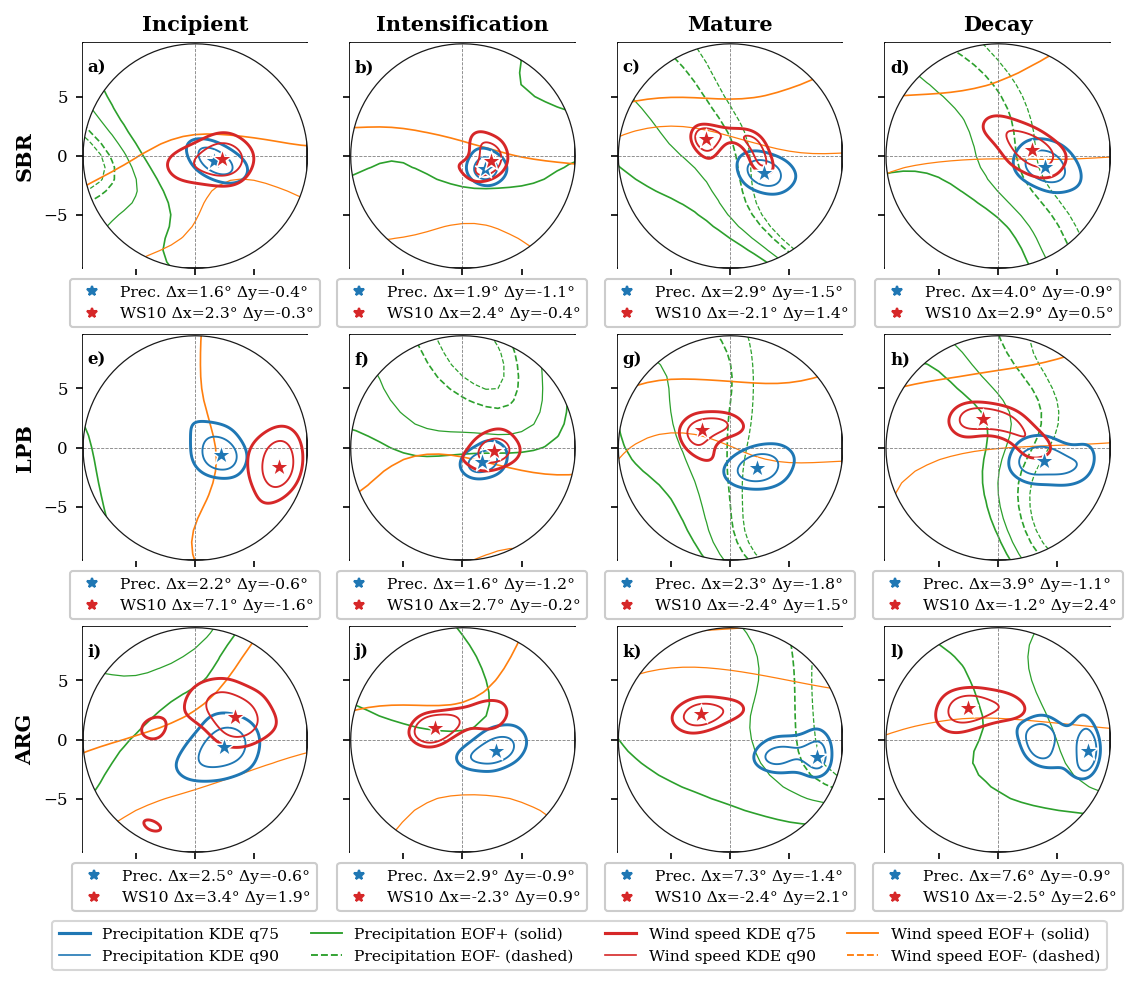
\includegraphics[width=\textwidth]{images/prototipos/prototipo_12panels_global.png}
\caption[Protótipos estruturais — População Global]{Protótipos estruturais para a População Global de ciclones extratropicais do Atlântico Sul-Ocidental. Cada painel superpõe, no domínio de $20^{\circ} \times 20^{\circ}$ centrado no sistema (0,0), os contornos PDFe dos quantis 75 e 90 de precipitação total (azul, linha grossa e fina respectivamente) e vento a 10 m (vermelho), juntamente com as cargas positivas (linha sólida) e negativas (linha pontilhada) do EOF1 de precipitação (verde) e vento (laranja). As estrelas azul e vermelha indicam as coordenadas modais ($\Delta x$, $\Delta y$) de cada campo. A matriz organiza as regiões de ciclogênese em linhas (SBR, LPB, ARG) e as fases evolutivas em colunas (Incipiente, Intensificação, Maturidade, Decaimento). A máscara circular delimita o domínio a um raio de $9{,}5^{\circ}$.}
\label{fig:prototipo_global}
\end{figure}

A Figura~\ref{fig:prototipo_global} apresenta os protótipos estruturais para a População Global, integrando a geometria probabilística dos máximos de ambas as variáveis com os padrões de maior variabilidade explicada (EOF1) para oferecer uma leitura simultânea da localização preferencial dos forçantes de precipitação e circulação ao longo do ciclo de vida.

Constrói-se a partir dos campos PDFe sobre a grade fixa centrada no sistema (Seção~\ref{subsec:kde_tp_global} para precipitação e Seção~\ref{sec:kde_espacial_global} para vento), combinados com o primeiro autovetor espacial das análises EOF independentes (Seção~\ref{sec:eof_tp} e Seção~\ref{sec:eof_wind10}). Os contornos de densidade são suavizados com um filtro gaussiano ($\sigma = 2$) antes de traçar os níveis dos quantis 75 e 90 segundo o critério de região de maior densidade (HDR). Seu propósito é sintetizar a coexistência ou diferenciação espacial entre circulação e precipitação nos ciclones ordinários, estabelecendo a linha de base em relação à qual será comparado o subconjunto de alta vorticidade na seção seguinte.

Durante as fases incipiente e intensificação (painéis a--f), os protótipos da População Global mostram uma colocalização relativa entre os máximos de precipitação e vento. Em SBR (painéis a--b), os contornos PDFe se superpõem parcialmente no quadrante oriental, com as modas de precipitação e vento separadas por apenas $0{,}1^{\circ}$--$0{,}7^{\circ}$ em latitude, enquanto as cargas do EOF1 de vento se estendem em direção ao noroeste. Em LPB (painéis e--f), tanto a precipitação quanto o vento se situam a leste-sudeste do centro durante a incipiência, com o vento sistematicamente mais afastado na componente zonal. A separação modal é de $4{,}9^{\circ}$ na fase incipiente (painel e) e se reduz a $1{,}1^{\circ}$ na intensificação (painel f). Em ARG (painéis i--j), o padrão já é bimodal desde as etapas iniciais. O PDFe de precipitação se mantém a leste-sudeste em ambas as fases, enquanto o de vento se desloca do nordeste (painel i) para o noroeste (painel j), antecipando a divergência que se consolida na maturidade. Essa colocalização parcial inicial reflete que, no regime médio, os forçantes frontais do WCB organizam ambos os campos no mesmo setor ativo do ciclone, antes que a diferenciação interna imponha geometrias distintas.

Ao transitar para a maturidade (painéis c, g, k) e o decaimento (painéis d, h, l), a arquitetura do protótipo se modifica de forma sistemática, ainda que moderada. Em LPB, os contornos PDFe de vento se deslocam em direção ao noroeste, coerentemente com a intensificação da circulação no flanco posterior do ciclone, enquanto os de precipitação se expandem em direção ao leste e sudeste, alcançando uma separação zonal de $4{,}7^{\circ}$ na maturidade (painel g) que se mantém em $5{,}1^{\circ}$ no decaimento (painel h). Em SBR, esse padrão é menos consistente. A separação zonal de $5{,}0^{\circ}$ observada na maturidade (painel c) se reduz a $1{,}1^{\circ}$ no decaimento (painel d), onde o vento retorna ao setor nordeste em vez de continuar se deslocando para o ocidente. No entanto, tanto os contornos PDFe quanto as cargas EOF1 mantêm, na População Global, uma extensão espacial considerável, sem que nenhum campo colapse para uma geometria estreita e bem definida, comportamento que reflete a heterogeneidade estrutural inerente ao catálogo completo, em que a integração de ciclones com diferentes taxas de oclusão, profundidades de vórtice e ambientes termodinâmicos dilui o sinal espacial de qualquer subconjunto estruturalmente coerente.

A comparação regional revela assimetrias na dinâmica de separação. Em ARG (painéis i--l), a divergência entre os PDFe de vento e precipitação é a mais pronunciada desde as fases iniciais, com a moda de vento deslocada para o noroeste ($\Delta x < 0$, $\Delta y > 0$) a partir da intensificação (painéis j--l), após iniciar a nordeste na fase incipiente (painel i, $\Delta x = 3{,}4^{\circ}$, $\Delta y = 1{,}9^{\circ}$), enquanto a moda de precipitação se mantém a leste-sudeste, com $\Delta x$ positivo e $\Delta y$ negativo nos quatro painéis. Esse comportamento contrasta com SBR e LPB, onde a separação meridional entre as modas é menor. Os contornos PDFe de precipitação de ARG, por sua vez, são os mais extensos das três regiões nas quatro fases. Essas diferenças regionais são coerentes com os padrões individuais descritos nos capítulos anteriores e confirmam que a síntese estrutural do protótipo não faz a média dessas diferenças, mas sim as preserva na leitura integrada.

\section{Subconjunto de alta vorticidade (p90)}\label{sec:prototipo_p90}

\begin{figure}[H]
\centering
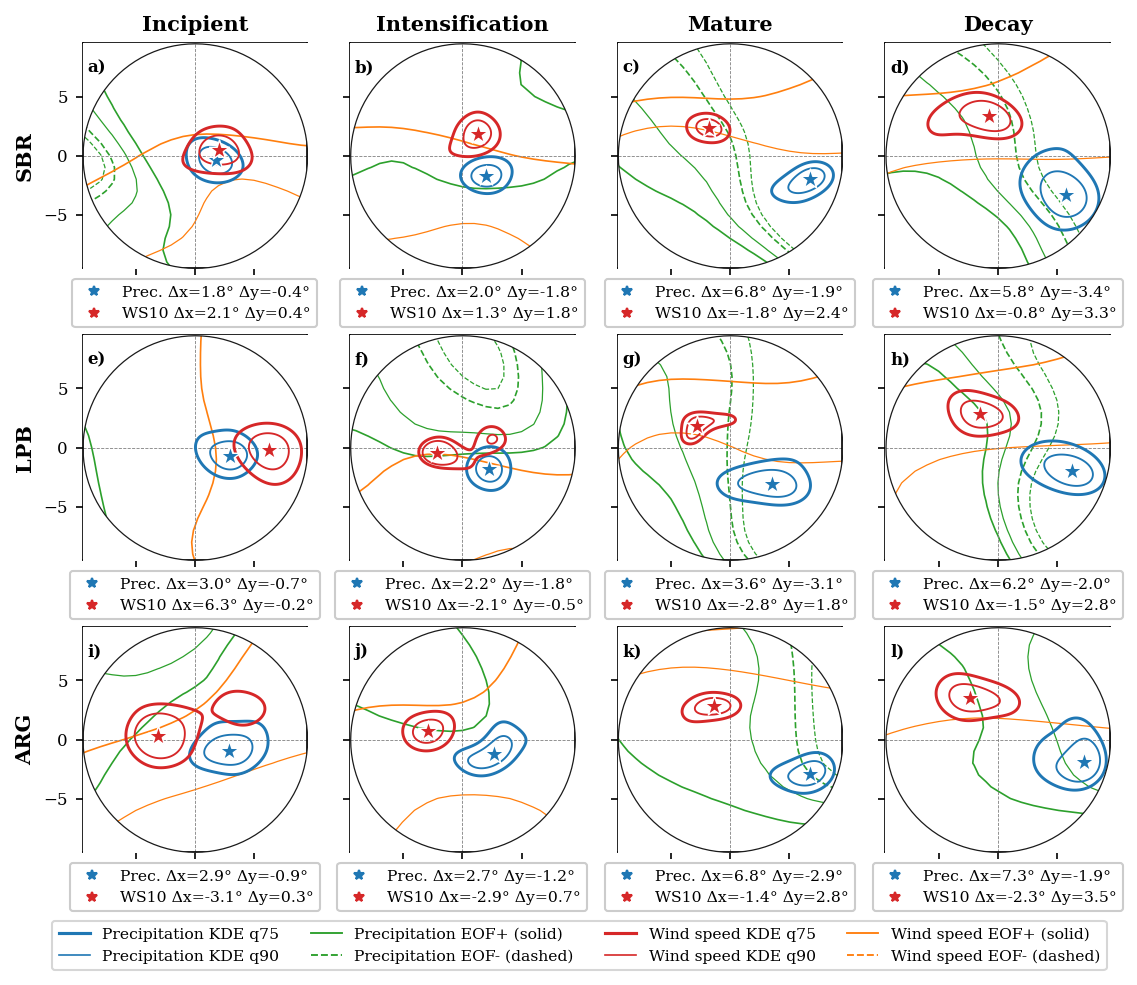
\includegraphics[width=\textwidth]{images/prototipos/prototipo_12panels_p90.png}
\caption[Protótipos estruturais — Subconjunto p90]{Protótipos estruturais para o subconjunto de ciclones de alta vorticidade (percentil 90 de vorticidade máxima). O formato dos painéis, a disposição matricial ($3 \times 4$, regiões $\times$ fases), a simbologia de cores e a escala do domínio centrado no sistema são idênticos aos da Figura~\ref{fig:prototipo_global}, permitindo quantificar diretamente a transformação estrutural que os sistemas p90 apresentam em relação à climatologia geral.}
\label{fig:prototipo_p90}
\end{figure}

A Figura~\ref{fig:prototipo_p90} apresenta os protótipos estruturais para o subconjunto de ciclones de alta vorticidade (p90), construídos com o mesmo procedimento metodológico da Figura~\ref{fig:prototipo_global}, mas restritos ao estrato de sistemas com vorticidade máxima no percentil 90. Essa visualização quantifica a diferenciação espacial entre circulação e precipitação nos sistemas p90 do Atlântico Sul-Ocidental, encerrando o argumento analítico desenvolvido nos capítulos de precipitação e vento. A comparação direta entre ambas as figuras, possível graças à escala, simbologia e disposição matricial idênticas, permite avaliar se a intensificação dinâmica amplifica ou reorganiza a disposição espacial relativa entre precipitação e vento.

O contraste visual com a População Global é imediato e profundo. Na fase de maturidade de SBR (painel c), o PDFe de precipitação (azul) entra em colapso em uma estrutura compacta deslocada para leste-sudeste ($\Delta x = 6{,}8^{\circ}$, $\Delta y = -1{,}9^{\circ}$), enquanto o PDFe de vento (vermelho) se concentra no quadrante noroeste ($\Delta x = -1{,}8^{\circ}$, $\Delta y = 2{,}4^{\circ}$). A separação entre ambas as modas é de ${\sim}9{,}5^{\circ}$ em distância euclidiana, em contraste com os ${\sim}5{,}8^{\circ}$ observados no mesmo painel (SBR, maturidade) da População Global. Essa diferença não é uniforme entre regiões e fases na População Global. Em SBR, a separação nas fases iniciais é mínima (painéis a-b, $0{,}7^{\circ}$--$0{,}9^{\circ}$), mas em LPB e ARG já se observam separações consideráveis mesmo na incipiência e na intensificação (até $5{,}5^{\circ}$ na intensificação de ARG, painel j), de modo que o contraste Global-vs-p90 é mais marcado em SBR do que nas outras duas regiões. Esse padrão de separação cruzada, precipitação a leste-sudeste, vento a noroeste, se reproduz com notória consistência em LPB (painéis g e h) e, com a maior magnitude das três regiões, em ARG (painéis k e l), onde a precipitação se desloca para leste ($\Delta x = 6{,}8^{\circ}$) e o vento mantém sua posição a noroeste ($\Delta x = -1{,}4^{\circ}$, $\Delta y = 2{,}8^{\circ}$), alcançando uma separação euclidiana próxima de $10^{\circ}$ na maturidade, que se amplia ainda mais no decaimento (painel l, ${\sim}11^{\circ}$), a maior de todo o subconjunto p90. Essa assinatura geométrica de quadrantes opostos constitui a expressão quantitativa da diferenciação espacial entre campos nos ciclones p90 da região.

A gênese dessa diferenciação nos sistemas de alta vorticidade poderia estar relacionada aos processos de oclusão documentados nas análises individuais de cada variável: a alta concentração do vento no quadrante noroeste, com densidades de até 27$\times10^{-4}$ em SBR e 23--25$\times10^{-4}$ em LPB (ARG se mantém mais baixa, ${\sim}19$--$21\times10^{-4}$; Seção~\ref{sec:kde_espacial_p90}), e a concentração do EOF1 de precipitação de até 36.5\% em LPB durante o decaimento (Seção~\ref{subsec:var_exp_tp}), são as duas faces quantitativas da mesma reorganização aqui sintetizada. O padrão de vento a noroeste é compatível com o ciclo de vida do tipo Shapiro-Keyser \citep{shapiro1990life}, no qual a cinta transportadora fria (\textit{cold conveyor belt}, CCB) se enrolaria em torno do núcleo do sistema em processo de oclusão, gerando o máximo de circulação de baixo nível no setor posterior do vórtice \citep{schemm2014linkage}. Simultaneamente, uma possível intrusão seca (\textit{dry intrusion}) proveniente da alta troposfera em direção ao núcleo do ciclone explicaria o espaço relativamente livre de precipitação que separa ambos os campos, embora esse mecanismo não seja medido diretamente em nenhum capítulo desta tese. O remanescente de umidade do WCB, por sua vez, é arrastado pela circulação ciclônica em direção à periferia, formando a estrutura em arco de precipitação no quadrante leste-sudeste, em uma posição mais próxima à do WCB do que à do quadrante ocluído que \citet{martin1999forcing} descreve para a banda enrolada (\textit{wrap-around precipitation}). A superposição desses dois processos, operando em quadrantes opostos, é o que gera a configuração diferenciada que o protótipo p90 capta.

A fase de decaimento (painéis d, h, l) mantém essa separação nas três regiões e a amplia em LPB e ARG. Em SBR (painel d), a moda de precipitação se desloca ainda mais para o sul ($\Delta x = 5{,}8^{\circ}$, $\Delta y = -3{,}4^{\circ}$) enquanto o vento migra para o norte ($\Delta x = -0{,}8^{\circ}$, $\Delta y = 3{,}3^{\circ}$), com uma separação euclidiana de ${\sim}9{,}3^{\circ}$, semelhante à da maturidade. Em LPB (painel h), os contornos PDFe de precipitação se estreitam em uma faixa arqueada em direção ao sul-sudeste, enquanto o vento mantém seu núcleo compacto a noroeste, com uma separação modal de $7{,}7^{\circ}$ na direção zonal. Esse comportamento reflete que, à medida que o ciclone se dissipa, a estrutura em arco mantém sua posição periférica mesmo quando a intensidade do sistema se debilita, enquanto o núcleo de vento se sustenta pela inércia ciclônica e pela advecção de vorticidade remanescente. As cargas do EOF1 de vento (laranja) mantêm sua orientação noroeste-sudoeste em todas as regiões durante o decaimento, enquanto as do EOF1 de precipitação (verde) adquirem uma curvatura arqueada para o sul, coerente com a geometria da faixa periférica documentada na Seção~\ref{subsec:eof1_tp_p90}.

As diferenças regionais na geometria da separação se manifestam primeiro na intensidade e extensão do campo de precipitação. Em SBR e LPB, a disponibilidade de umidade tropical canalizada pelo SALLJ \citep{reboita2026meteorology} poderia sustentar a estrutura em arco de precipitação com maior intensidade, aumentando a densidade no quadrante sudeste e ampliando a zona de alta probabilidade na maturidade e no decaimento. Em ARG (painéis i--l), a correlação entre o PC1 de precipitação e a vorticidade se mantém significativa durante todo o ciclo de vida em p90, incluindo a maturidade (Capítulo~\ref{cap:resultados_tp}), diferentemente de SBR e LPB, onde essa correlação deixa de ser significativa nessa fase, o que poderia explicar que a moda de precipitação mantenha, entre a maturidade e o decaimento, a posição mais estável das três regiões (deslocamento de ${\sim}1^{\circ}$, frente a ${\sim}1{,}7^{\circ}$ em SBR e ${\sim}2{,}9^{\circ}$ em LPB). No entanto, a separação euclidiana entre as modas de vento e precipitação não é menor do que em SBR e LPB, mas sim a maior das três regiões (${\sim}10$--$11^{\circ}$ na maturidade e no decaimento, contra ${\sim}9$--$9{,}5^{\circ}$ em SBR e ${\sim}8$--$9^{\circ}$ em LPB). A direção da diferenciação, precipitação a leste-sudeste, vento a noroeste, mantém-se sim consistente nas três regiões, revelando que a topologia fundamental da reorganização espacial é comum às três regiões, enquanto sua magnitude responde a uma combinação de fatores regionais que este capítulo não consegue atribuir de forma inequívoca ao regime de umidade oceânica.

A fase incipiente dos ciclones de alta vorticidade (painéis a, e, i) mostra que a diferenciação ainda não está plenamente desenvolvida, mas já exibe uma tendência diferenciada em relação à População Global equivalente. Em SBR (painel a), a moda de vento a nordeste ($\Delta x = 2{,}1^{\circ}$, $\Delta y = 0{,}4^{\circ}$) se separa levemente da moda de precipitação a leste ($\Delta x = 1{,}8^{\circ}$, $\Delta y = -0{,}4^{\circ}$), com os contornos PDFe ainda parcialmente superpostos, mas com centros diferenciados; a orientação para noroeste que caracterizará o vento em fases posteriores ainda não se manifesta nesta etapa incipiente. Em LPB (painel e), a separação zonal é mais notável desde o início ($\Delta x_{\text{vento}} = 6{,}3^{\circ}$, $\Delta x_{\text{prec}} = 3{,}0^{\circ}$), refletindo que os sistemas que eventualmente alcançarão o percentil 90 de vorticidade já exibem, durante sua gênese, uma assimetria frontal mais pronunciada do que a média, coerente com o maior gradiente térmico e o maior fluxo de umidade que caracteriza esses ambientes de ciclogênese mais ativos.

% SEÇÃO: DISCUSSÃO
\section{Discussão}\label{sec:discusion_prototipos}

% --- PARÁGRAFO 1: Validação da abordagem centrada no sistema e comparação com a literatura ---

A colocalização parcial documentada nos protótipos da População Global durante as fases incipiente e intensificação --consistente com o pico modal simultâneo de vento (12--15~m\,s$^{-1}$) e precipitação (10--20~mm/h) já relatado nessa mesma fase (Seções~\ref{sec:pdf_wind10} e~\ref{sec:pdf_tp})-- é coerente com os resultados de \citet{cardoso2022synoptic} para ciclones subtropicais do Atlântico Sul, uma estrutura geralmente distinta dos ETC baroclínicos catalogados nesta tese, que, por meio de um referencial lagrangiano semelhante, com um domínio de $20^{\circ} \times 20^{\circ}$ que acompanha o centro do ciclone, identificam anomalias positivas de vento a leste e nordeste da região ciclogenética RG1 e de precipitação a leste e dentro dela, calculadas pela média ao longo do ciclo de vida. Os protótipos do presente trabalho estendem esse resultado de duas maneiras: primeiro, ao incorporar explicitamente a fase evolutiva como eixo de estratificação, mostram que essa colocalização é própria das fases iniciais e não uma propriedade estática do ciclone; segundo, ao contrastar a População Global com o subconjunto p90, mostram que a colocalização se rompe de maneira quantificável nos sistemas p90. Essa distinção não pode ser inferida das análises climatológicas que calculam a média sobre o ciclo de vida completo \citep{gramcianinov2023impact}, e constitui o valor agregado central da abordagem de protótipos condicionais adotada nesta tese.

% --- PARÁGRAFO 2: A separação espacial em p90 e o modelo Shapiro-Keyser ---

A separação de quadrantes nos protótipos p90, vento a noroeste, precipitação a sudeste e sul, é compatível com a transição para o modelo de Shapiro-Keyser \citep{shapiro1990life}. Essa interpretação se apoia em um modelo conceitual geral, sem um estudo equivalente para o Atlântico Sul que confirme diretamente a sequência completa de oclusão nessa região.

% --- PARÁGRAFO 3: Comparação com estudos do Hemisfério Norte e transferibilidade do referencial conceitual ---

A arquitetura de quadrantes documentada nos protótipos p90 do Hemisfério Sul guarda certa correspondência, embora especulativa, com a organização do campo de vento relatada para ciclones explosivos do Hemisfério Norte. \citet{priestley2022improved} compõem os sistemas do percentil 90 de vorticidade ciclônica no ERA5 sobre um domínio de ${\sim}20^{\circ}$ centrado na trajetória, critério e escala comparáveis aos deste trabalho, e constatam que os ventos associados à CCB se concentram no flanco posterior-ocidental do vórtice; por inversão da circulação ciclônica entre hemisférios, essa posição é topologicamente análoga à concentração noroeste do vento documentada aqui. Cabe precisar que esse estudo não analisa o campo de precipitação, de modo que a comparação se limita estritamente ao vento. Isso sugere que a organização do vento em quadrantes opostos ao forçante do WCB é um traço compartilhado entre hemisférios, enquanto a geometria da estrutura em arco de precipitação do Atlântico Sul não tem um análogo conjunto vento-precipitação documentado na literatura do Hemisfério Norte consultada aqui.

% --- PARÁGRAFO 4: Os protótipos como ferramenta de diagnóstico: vínculo com o referencial multivariado ---

A abordagem de protótipos estruturais desenvolvida neste capítulo se alinha metodologicamente com propostas recentes que enfatizam a necessidade de vincular explicitamente a evolução dinâmica do sistema às suas manifestações estruturais. \citet{han2025system} propõem o \textit{SyCLoPS}, um referencial de classificação objetiva de alcance global que distingue dezesseis classes de sistemas de baixa pressão, incluindo os ciclones extratropicais como a classe mais frequente de seu catálogo. No entanto, seu referencial reserva a designação de sistemas de \textit{alto impacto}, e os composites de estrutura, precipitação e energia cinética associados a essa designação, aos ciclones tropicais, subtropicais e baixas polares, sem incluir os ciclones extratropicais nessa análise, apesar de serem a classe mais frequente de seu catálogo. Os protótipos apresentados neste capítulo abordam essa lacuna para o Atlântico Sul, quantificando, por meio de densidades de probabilidade espacial e modos dominantes de variabilidade (EOF), a posição relativa dos máximos de vento e precipitação em relação ao centro do vórtice, em um domínio centrado no sistema padronizado que permite a comparação direta entre regiões e fases do ciclo de vida. Essa abordagem revela, para os ciclones extratropicais da região, uma reorganização geométrica horizontal entre ambos os campos que um composite de corte vertical não capta diretamente. Essa combinação de geometria modal e densidade probabilística constitui, assim como o referencial proposto por \citet{corner2025classification} por meio de análise multivariada de parâmetros dinâmicos, um avanço em direção à caracterização objetiva e quantificada dos sistemas intensos ($\zeta_{850}$) no Atlântico Sul, uma região onde estudos equivalentes permaneceram, até agora, muito limitados.

% --- PARÁGRAFO 5: Limitações da abordagem e perspectivas futuras ---

Duas limitações da abordagem de protótipos merecem discussão explícita. Em primeiro lugar, a padronização do domínio centrado no sistema em uma grade fixa de $\pm 9{,}5^{\circ}$ implica que sistemas cuja estrutura em arco de precipitação se estende além desse raio, possível nos ciclones de maior escala horizontal, contribuem com densidade PDFe truncada nas bordas do domínio, subestimando a extensão real do campo de precipitação no protótipo. Essa limitação é inerente à abordagem composta centrada e foi reconhecida por \citet{cardoso2022synoptic}, que adotam explicitamente um domínio de $20^{\circ} \times 20^{\circ}$ precisamente para capturar os ventos extremos que podem ocorrer até 500 km do centro do ciclone. Em segundo lugar, a construção dos protótipos sobre o subconjunto estático p90 de vorticidade máxima implica que a amostra inclui sistemas em diferentes fases de seu ciclo de vida no momento de serem catalogados, embora a estratificação por fases mediante o algoritmo \textit{CycloPhaser} \citep{deSouza2025CycloPhaser} mitigue, em grande medida, esse efeito ao garantir que cada instante analisado pertença à fase correta do ciclone individual. Essas limitações abrem linhas de trabalho futuro: a extensão do domínio a $30^{\circ} \times 30^{\circ}$ para ciclones de grande escala, e a estratificação adicional pela velocidade de translação do sistema, um fator que, como apontam \citet{gramcianinov2023impact}, modula diretamente a duração do forçante e a extensão espacial dos campos dinâmicos, permitiriam refinar os protótipos em direção a representações mais completas da diversidade estrutural dos ciclones de alta vorticidade do Atlântico Sul.

\section{Síntese}\label{sec:sintesis_prototipos}

Os protótipos estruturais sintetizam, em uma representação geométrica única, a evolução diferencial da organização espacial dos campos de precipitação e vento associada aos ciclones extratropicais do Atlântico Sul-Ocidental ao longo de seu ciclo de vida. Na População Global, durante as fases incipiente e intensificação, as modas de precipitação e vento situam-se ambas no setor oriental em SBR e LPB, enquanto em ARG o vento já se desloca para noroeste na intensificação. Rumo à maturidade os campos se separam nas três regiões, embora em SBR a separação volte a diminuir no decaimento, e os contornos mantêm geometrias difusas que refletem a heterogeneidade da população geral.

Em contraste, o protótipo p90 revela uma reorganização qualitativa compatível com um processo de oclusão avançado. A superposição simultânea dos PDFe e EOF1 de ambas as variáveis no mesmo domínio quantifica a diferenciação espacial em sua expressão mais nítida. Os sistemas de alta vorticidade maduros e em decaimento apresentam os máximos de vento concentrados no quadrante noroeste, na zona onde a literatura situa a cinta transportadora fria, enquanto os máximos de precipitação ficam a leste-sudeste, na estrutura em arco. Em SBR e LPB, a separação entre modas na maturidade e no decaimento (${\sim}8$--$9{,}5^{\circ}$) supera claramente a da População Global (${\sim}2$--$6^{\circ}$). Em ARG, a separação é a maior das três regiões em p90 (${\sim}10$--$11^{\circ}$), mas é semelhante à de sua População Global, de modo que nessa região ela não é exclusiva dos sistemas mais intensos.

Do ponto de vista da dinâmica sinótica, esse resultado implica que os sistemas de alta vorticidade do Atlântico Sul não podem ser caracterizados pela colocalização simplificada de seus campos de precipitação e circulação. O centro de máxima variabilidade de precipitação e o centro de máxima variabilidade de vento operam em quadrantes opostos em relação ao centro do vórtice, com uma defasagem espacial que aumenta rumo à maturidade e ao decaimento. Em conclusão, os protótipos apresentados neste capítulo constituem a síntese espacial dos padrões dominantes de variabilidade de cada campo (EOF1 univariados) e de sua densidade de ocorrência (PDFe), consistente com dois resultados independentes dos capítulos anteriores. Primeiro, em p90-maturidade a vorticidade continua se correlacionando significativamente com a estrutura do vento nas três regiões ($|r|$ entre $0.26$ e $0.74$, Capítulo~\ref{cap:resultados_wind10}), enquanto para a precipitação essa correlação deixa de ser significativa em SBR e LPB ($|r|=0.17$ e $0.03$) e só se mantém em ARG ($|r|=0.24$, Capítulo~\ref{cap:resultados_tp}), o que sugere que a intensidade do vórtice deixa de prever a organização da precipitação com a mesma força com que continua prevendo a do vento. Segundo, a correlação entre as PC1 univariadas de precipitação e vento durante a maturidade em p90 é significativa nas três regiões ($|r|$ entre $0.31$ e $0.45$, Capítulo~\ref{chap:meof}), e sua relação com a localização real de cada EOF1 mostra que os eventos de um ciclo de vida que mais projetam sobre a estrutura em arco de precipitação tendem a ser os que menos projetam sobre o núcleo de vento. Essa separação de quadrantes é compatível com a reorganização do vórtice durante a oclusão, em que uma possível intrusão seca deslocaria a convecção para a periferia enquanto a cinta transportadora fria consolidaria a circulação de baixo nível no setor posterior.
		% trabalho.
\chapter{Conclusões}\label{ch:conclusiones}

Esta tese perguntou como evolui espacialmente a distribuição de vento e precipitação nos ciclones extratropicais do Atlântico Sul, e quais configurações caracterizam essa organização nas fases incipiente, intensificação, maturidade e decaimento. A resposta depende da intensidade do sistema. Na População Global, ambos os campos compartilham o flanco oriental do ciclone durante as fases iniciais e depois se dispersam sem se reorganizar. No subconjunto de maior vorticidade (p90), por sua vez, a partir da maturidade os máximos de vento se concentram ao noroeste e os de precipitação a leste e sudeste, em uma estrutura em arco afastada do centro, com separações superiores a $8^{\circ}$ nas três regiões de gênese.

A hipótese formulada se confirma no essencial. As assimetrias de ambos os campos variam entre fases e entre estratos de intensidade. Entre regiões, a direção da separação se mantém e o que varia é sua magnitude. A segunda parte da hipótese, de que esses padrões não são capturáveis mediante métricas escalares de intensidade central, se cumpre com clareza para a precipitação, cuja relação com a vorticidade deixa de ser significativa na maturidade dos sistemas p90 de SBR e LPB. Para o vento, cumpre-se apenas em parte, já que seu modo dominante permanece correlacionado com a vorticidade em p90, embora esse modo já não descreva por si só a variabilidade do campo. As seções seguintes apresentam os resultados que sustentam essa resposta, na ordem dos objetivos específicos.

\section{Base de dados semilagrangeana (Objetivo Específico 1)}

Construiu-se uma base de dados semilagrangeana que associa os campos horários de vento a 10~m e precipitação total do ERA5 com as trajetórias de \citet{gramcianinov2020analysis} e com a classificação objetiva de fases do \textit{CycloPhaser} \citep{coutodesouza2024new, deSouza2025CycloPhaser}, conservando unicamente os sistemas com ciclo de vida completo. A amostra foi estratificada por região de gênese (SBR, LPB e ARG) e por intensidade dinâmica ($\zeta_{850}^{\min}$), na População Global e no subconjunto p90. A classificação de fases é coerente com a dinâmica dos sistemas, já que 83\% dos ciclones p90 e 72\% da População Global alcançam seu mínimo de vorticidade durante a maturidade. Essa coerência permite comparar os padrões espaciais fase por fase sem que a atribuição de fases introduza uma defasagem sistemática.

\section{Magnitude e localização dos máximos (Objetivo Específico 2)}

Em magnitude, o vento separa com clareza ambas as populações à medida que os sistemas maturam. Na maturidade, a moda dos máximos de vento de p90 situa-se entre 23 e 25~m\,s$^{-1}$, entre 25\% e 50\% acima da População Global (16--19~m\,s$^{-1}$), com caudas de até 30~m\,s$^{-1}$. A precipitação se comporta de outra forma. Nas fases iniciais, p90 se desloca apenas levemente para valores maiores (${\sim}25$~mm\,h$^{-1}$ em SBR incipiente e ${\sim}30$~mm\,h$^{-1}$ em LPB intensificação), e as taxas superiores a 60~mm\,h$^{-1}$ não são exclusivas de p90. Na maturidade a relação se inverte, e a moda de p90 em SBR (${\sim}7$~mm\,h$^{-1}$) fica abaixo da População Global (${\sim}17$~mm\,h$^{-1}$), até se concentrar em 1--4~mm\,h$^{-1}$ no decaimento de SBR e LPB. ARG apresenta as menores taxas de precipitação em todas as fases. A partir da maturidade, portanto, pertencer a p90 implica ventos mais intensos, mas não maior precipitação.

Em localização, a População Global mostra distribuições amplas e de gradientes suaves. Os máximos de vento passam do setor leste nas primeiras fases para o quadrante noroeste na maturidade, e os de precipitação mantêm uma assimetria persistente para leste e sudeste, na posição que a literatura atribui ao WCB. Em p90 essa organização se torna mais compacta. Na maturidade, os máximos de vento se concentram no quadrante noroeste, a ${\sim}2$--$4^{\circ}$ do centro, com densidades de 19--27$\times10^{-4}$ frente a 11--15$\times10^{-4}$ na População Global, na zona onde a literatura situa a esteira transportadora fria (CCB) e a fratura frontal. Os máximos de precipitação, por sua vez, se afastam do centro e se confinam em faixas alongadas a leste e sudeste, que persistem no decaimento enquanto na População Global o sinal se dissipa. A concentração do vento é maior em SBR e LPB do que em ARG, embora SBR apresente a distribuição de magnitudes mais larga, de modo que a região que mais concentra a localização de seus máximos não é a que mais concentra sua intensidade.

\section{Modos dominantes de variabilidade (Objetivo Específico 3)}

A análise EOF univariada mostra que a intensidade muda a forma como se distribui a variabilidade de cada campo, e que o faz em sentidos opostos. Na População Global, o EOF1 de vento explica entre 30.9\% e 57.4\% da variância, é significativo em todo o domínio e sua PC1 se correlaciona com a vorticidade até $|r|=0.86$--$0.89$ na maturidade. Em p90, o EOF1 de vento não supera 37.6\% e a variância se distribui entre vários modos. Sua PC1 permanece correlacionada de forma significativa com a vorticidade ($|r|$ entre $0.26$ e $0.74$), mas PC2 e PC3 superam PC1 em quatro combinações de região e fase (até $|r|=0.58$ em SBR), o que é compatível com um maior peso da variabilidade de mesoescala nos ciclones intensos. A precipitação segue o caminho inverso. Na População Global sua variabilidade se dispersa entre múltiplos modos (EOF1 entre 11.1\% e 16.4\%), enquanto em p90 o EOF1 se concentra na maturidade e no decaimento, até 36.5\% em LPB e 26.2\% em SBR durante o decaimento. Nessas mesmas fases, a correlação de sua PC1 com a vorticidade deixa de ser significativa em SBR ($|r|=0.17$) e LPB ($|r|=0.03$) durante a maturidade e só se mantém em ARG ($|r|=0.24$).

A análise multivariada (MEOF) avalia se essas transformações se refletem na covariabilidade conjunta de ambos os campos. Na População Global, o MEOF1 captura entre 14.8\% e 26.6\% da covariância conjunta, com gradientes de precipitação e vento orientados em eixos distintos (oeste-leste e norte-sul, respectivamente). Em p90, essa fração cai para 11.65\%--23.47\% e, na maturidade, o MEOF1 mostra um padrão de anticovariância com as cargas de precipitação a sudeste e as de vento a oeste. Esse resultado tem uma ressalva importante. O vento domina o MEOF1 na maioria das combinações de região, fase e população, e a precipitação só contribui com força comparável em p90 a partir da maturidade. O padrão de anticovariância é, portanto, interpretável sobretudo nessa combinação. Ali, a correlação significativa entre as PC1 univariadas de ambos os campos ($|r|$ entre $0.31$ e $0.45$ nas três regiões) é consistente com a separação geométrica, já que os eventos que mais projetam sobre a estrutura em arco de precipitação tendem a ser os que menos projetam sobre o núcleo de vento.

\section{Protótipos estruturais (Objetivo Específico 4)}

Os protótipos estruturais, que sobrepõem em um mesmo painel as PDFe e o EOF1 univariado de ambas as variáveis, convertem os resultados anteriores em distâncias concretas entre os máximos de cada campo. Na População Global, as separações modais durante as fases iniciais são pequenas em SBR (abaixo de $1^{\circ}$) e moderadas em LPB e ARG (até $4{,}9^{\circ}$ e $5{,}5^{\circ}$, respectivamente), e na maturidade e no decaimento os contornos permanecem extensos, sem que nenhum campo adote uma geometria bem definida, embora em ARG as modas já se separem ${\sim}10^{\circ}$. Em p90, na maturidade de SBR, a moda de precipitação ($\Delta x = 6{,}8^{\circ}$, $\Delta y = -1{,}9^{\circ}$) e a de vento ($\Delta x = -1{,}8^{\circ}$, $\Delta y = 2{,}4^{\circ}$) ficam separadas ${\sim}9{,}5^{\circ}$, distância que se mantém no decaimento. LPB apresenta separações um pouco menores (${\sim}8$--$9^{\circ}$) e ARG as maiores (${\sim}10$--$11^{\circ}$).

A direção da separação, precipitação a leste-sudeste e vento a noroeste, se repete nas três regiões, enquanto sua magnitude varia sem que esta tese identifique um único fator regional que a explique. Em SBR e LPB, a umidade canalizada pelo Jato de Camadas Baixas da América do Sul (SALLJ) poderia sustentar a estrutura em arco com maior intensidade. ARG, onde a correlação entre o PC1 de precipitação e a vorticidade se mantém significativa durante todo o ciclo de vida em p90, apresenta no entanto a maior separação das três regiões. Essa configuração é compatível com a transição ao modelo de Shapiro-Keyser, na qual uma possível intrusão seca separaria ambos os campos, embora esse mecanismo não seja medido diretamente nesta tese e sua interpretação se apoie em estudos do Hemisfério Norte.

Em síntese, em resposta ao objetivo geral, a estrutura espacial do vento e da precipitação nos ciclones extratropicais do Atlântico Sul evolui de forma distinta segundo a intensidade do sistema. Nos ciclones de maior vorticidade, os máximos de ambos os campos terminam em setores opostos durante a maturidade e o decaimento, uma configuração que a média da População Global não mostra e que a vorticidade do centro, por si só, não descreve, o que é relevante para o risco costeiro.
		%
\chapter{Considerações Finais}\label{cap:Considerações}

\section{Contribuição e alcance}

Esta tese combina densidade espacial (PDFe), EOF univariado e MEOF para quantificar, por fase do ciclo de vida e região de gênese, a separação espacial entre vento e precipitação nos ciclones extratropicais do Atlântico Sul-Ocidental. A constatação central, de que a intensidade dinâmica do vórtice deixa de predizer linearmente a magnitude e a localização de seus impactos de superfície no subconjunto p90, e seu respaldo estatístico e geográfico, já foram desenvolvidos no Capítulo~\ref{ch:conclusiones}. A confiança de que esses padrões espaciais não são artefatos da amostragem se sustenta na reamostragem Bootstrap-t (Seção~\ref{subsec:bootstrap_significancia}), que documenta áreas estatisticamente significativas no EOF1 tanto na População Global quanto no subconjunto p90, estendendo-se neste último também ao EOF2 e EOF3, os mesmos modos que capturam a reorganização de mesoescala nos sistemas intensos, em alguns casos com maior área significativa que o próprio EOF1, o que respalda que o sinal relatado é físico e recorrente, e não ruído estocástico. As limitações e linhas futuras que seguem delimitam o alcance do que foi apresentado neste capítulo.

\section{Limitações}

Os resultados estão sujeitos à subestimação do ERA5 em extremos ($-10.2\%$ em vento e $-22.6\%$ em precipitação para os ciclones mais intensos), de modo que as magnitudes absolutas do subconjunto p90 são estimativas conservadoras. As estruturas de mesoescala responsáveis pelos máximos de vento em ciclones severos, como a CCB, os \textit{sting jets} ou as descargas descendentes, operam em escalas menores que a resolução do ERA5 ($\sim$31~km), limitando a resolução de sua geometria interna nos protótipos. A padronização do domínio centrado no ciclone em $\pm 9{,}5^{\circ}$ pode truncar a estrutura em arco de precipitação nos ciclones de maior escala horizontal, subestimando a extensão real do campo pluviométrico periférico.

O tamanho amostral do subconjunto p90 difere substancialmente entre regiões (198 ciclones em ARG, frente a 64 em SBR e 67 em LPB), de modo que as densidades periféricas das PDFe e os autovetores do EOF em SBR e LPB estão sujeitos a maior incerteza de amostragem que os de ARG. A avaliação de significância estatística mediante Bootstrap-t se concentrou na fase de maturidade, o momento de maior interesse para o argumento central da tese, de modo que os padrões EOF das fases restantes são apresentados como caracterização descritiva sem a mesma validação formal, e o modo multivariado (MEOF) se apoia na significância já estabelecida de seus componentes univariados na maturidade sem um teste multivariado independente. O próprio EOF, por ser uma decomposição linear, poderia diluir em um único modo diferenças que na realidade correspondam a subpopulações de ciclones estruturalmente discretas, embora o aplanamento do espectro de autovalores observado nos sistemas p90 sugira que o método está capturando, e não ocultando, essa complexidade.

A análise se circunscreve aos campos de superfície. A extensão à coluna tridimensional permitiria vincular as estruturas identificadas com seus mecanismos geradores.

O catálogo de trajetórias empregado \citep{gramcianinov2020analysis} constitui uma única fonte de detecção e rastreamento entre vários esquemas objetivos disponíveis para o Atlântico Sul (Seção~\ref{sec:tb_vorticidad}); embora baseado em vorticidade relativa a 850~hPa, um critério amplamente validado, não se pode descartar que outro catálogo modifique a composição exata das populações PG e p90. Espera-se, no entanto, que os sinais estruturais aqui documentados (a separação em quadrantes, a fragmentação do espectro de autovalores em p90) sejam robustos frente a essa escolha, na medida em que dependem da física do ciclone e não do algoritmo de detecção particular.

Diferentemente de estudos do Hemisfério Norte que rotacionam cada composite para alinhar a direção de deslocamento do sistema, por exemplo em direção ao leste, antes de calcular a média \citep{rudeva2011composite, priestley2022improved}, o referencial centrado no sistema aqui empregado mantém a orientação geográfica original (Seção~\ref{subsec:tb_lagrangiano}). Essa escolha preserva a interpretação direta dos quadrantes em termos cardinais (noroeste, sudeste), mas não corrige a variabilidade na direção de translação dos ciclones, o que poderia diluir, nunca exagerar artificialmente, as assimetrias estruturais relatadas; que estas emerjam com clareza apesar dessa fonte adicional de dispersão respalda a robustez do sinal detectado.

Adicionalmente, a exigência de um ciclo de vida completo com as quatro fases e sem reintensificações (Seção~\ref{subsec:grupo_global}) exclui sistemas de evolução complexa, truncada ou de vida curta, que poderiam representar uma fração não desprezível dos ETC reais da região. Os resultados aqui obtidos caracterizam, portanto, o subconjunto de ciclones com evolução estruturalmente completa, não a totalidade da atividade ciclônica do Atlântico Sul-Ocidental.

\section{Perspectivas futuras}

Como linhas futuras, seria possível validar a geometria dos protótipos com observações de alta resolução (boias, estações costeiras, satélites) para ajustar os vieses do ERA5 no subconjunto p90; incorporar vento vetorial em 850~hPa, temperatura potencial equivalente e vorticidade potencial à análise MEOF permitiria relacionar os padrões de superfície com sua evolução em altura, incluindo as correntes transportadoras (WCB, CCB) e o \textit{sting jet}; os protótipos também serviriam para definir limiares combinados de vento e precipitação e estimar a probabilidade de impactos conjuntos nas costas do Brasil, Uruguai e Argentina, distinguindo o perigo do vento (noroeste) do da chuva (sudeste-sul) segundo a posição do ciclone em relação à costa; simulações de alta resolução com diferentes cenários climáticos permitiriam avaliar se o aquecimento global modifica a separação de quadrantes aqui documentada; e estender a reamostragem Bootstrap-t a todas as fases do ciclo de vida e ao MEOF, junto com um registro mais longo ou dados de modelos de alta resolução para SBR e LPB, reduziria a incerteza de amostragem frente a ARG.
		%
       						%
						%
%\begin{thebibliography}{99}	% referências bibliográficas (dê
%\input{tex/bibliografia.tex} 	% preferência ao bibTeX).
%\end{thebibliography}		% caso não use o bibTeX, remova os
						% comentarios das três linhas
						% e comente a linha \bibliography
						%
\bibliography{tex/bibliografia}	% bibliografia utilizando bibTeX,
						% referente ao arquivo
						% bibliografia.bib na pasta tex/
						%
\begin{apendice}			% inicio do ambiente apendice
% % --- apendices.tex ---

% ==============================================================================
% KDE - APÉNDICE
% ==============================================================================

\chapter{Mapas complementares de densidade espacial KDE}\label{apendice:kde_espacial}

Neste apêndice documentam-se os campos de estimação de densidade espacial bidimensional (KDE) correspondentes aos estratos de intensidade inferior (p10 e p50), complementando a análise principal de assimetria espacial abordada no corpo do documento. Esses mapas evidenciam que os ciclones com menor forçante dinâmico estrutural carecem dos focos localizados observados nos sistemas extremos.

\section{Vento a 10 metros}\label{apendice:kde_wind10}

\subsection{Sistemas fracos (p10)}\label{apendice:kde_wind10_p10}
\begin{figure}[htbp]
\centering
\includegraphics[width=\textwidth]{images/w10/kde_wind10_p10_fasesxreg.png}
\caption[KDE espacial de vento a 10 m - Subconjunto p10]{Estimação de densidade espacial bidimensional (KDE) para a localização dos máximos de magnitude de vento a 10 metros no estrato de ciclones fracos (percentil 10). A topologia marcadamente dispersa ao longo de todo o ciclo de vida corrobora que, diante de vórtices com forçante dinâmico pobre desde sua gênese, a localização do vento máximo carece de organização de mesoescala e fica completamente subordinada às flutuações do fluxo sinótico de fundo.}
\label{fig:kde_wind10_p10_ap}
\end{figure}

\subsection{Sistemas moderados (p50)}\label{apendice:kde_wind10_p50}
\begin{figure}[htbp]
\centering
\includegraphics[width=\textwidth]{images/w10/kde_wind10_p50_fasesxreg.png}
\caption[KDE espacial de vento a 10 m - Subconjunto p50]{Estimação de densidade espacial bidimensional (KDE) para a localização dos máximos de magnitude de vento a 10 metros no estrato de ciclones típicos ou moderados (percentil 50). O mapa evidencia um grau de organização intermediário: durante a maturidade, os núcleos de máxima probabilidade começam a se agrupar debilmente nos quadrantes ocidentais, mostrando uma arquitetura um pouco mais definida que a dos sistemas fracos, mas sem jamais alcançar a alta concentração própria dos eventos severos.}
\label{fig:kde_wind10_p50_ap}
\end{figure}

% % \section{Viento a 100 metros}\label{apendice:kde_wind100}
% \section{Viento a 100 metros}\label{apendice:kde_wind100}

% \subsection{Sistemas débiles (p10)}\label{apendice:kde_wind100_p10}
% \begin{figure}[htbp]
% \centering
% \includegraphics[width=\textwidth]{images/w100/kde_wind100_p10_fasesxreg.png}
% \caption[KDE espacial de viento a 100 m - Subconjunto p10]{Estimación de densidad espacial bidimensional (KDE) para la ubicación de los máximos de magnitud de viento a 100 metros en el estrato de ciclones débiles (percentil 10). Al operar cerca del tope de la capa de Ekman y con un forzante dinámico pobre, la topología es extremadamente dispersa. La ubicación del viento máximo en estos sistemas carece de organización mesoescalar y queda completamente dictada por las amplias fluctuaciones del flujo sinóptico de fondo.}
% \label{fig:kde_wind100_p10_ap}
% \end{figure}

% \subsection{Sistemas moderados (p50)}\label{apendice:kde_wind100_p50}
% \begin{figure}[htbp]
% \centering
% 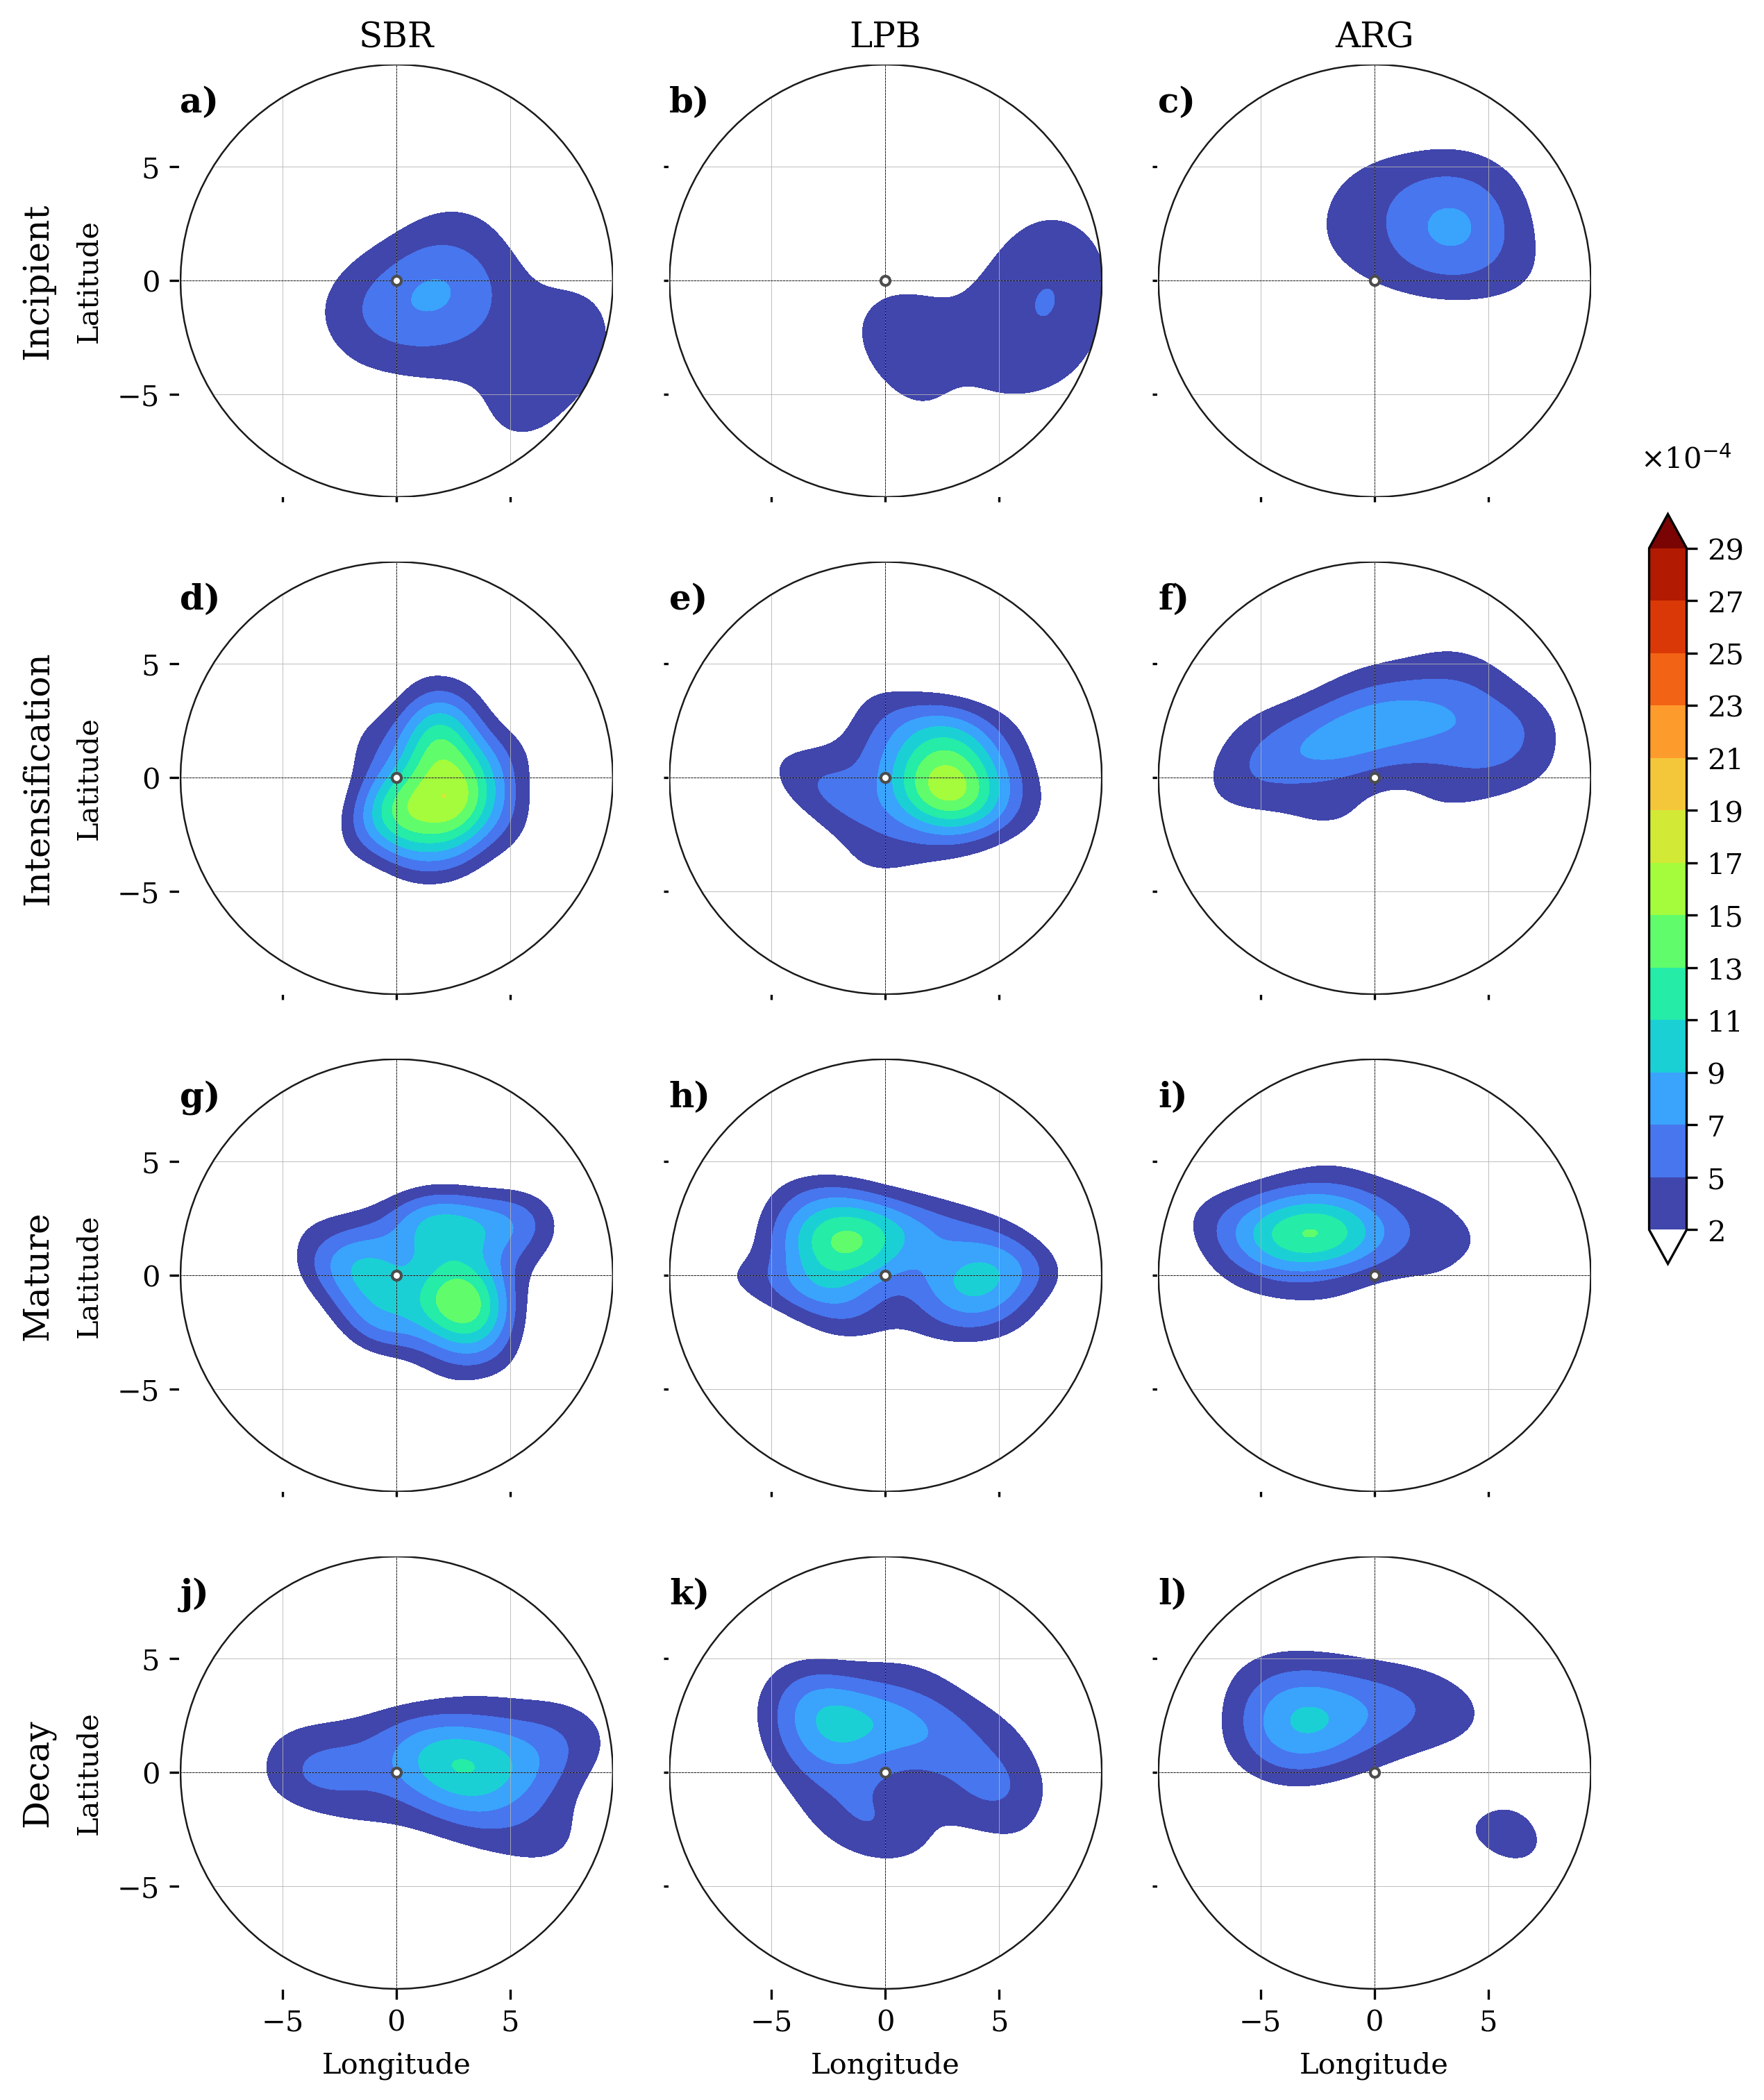
\includegraphics[width=\textwidth]{images/w100/kde_wind100_p50_fasesxreg.png}
% \caption[KDE espacial de viento a 100 m - Subconjunto p50]{Estimación de densidad espacial bidimensional (KDE) para la ubicación de los máximos de magnitud de viento a 100 metros en el estrato de ciclones moderados (percentil 50). El mapa evidencia un grado de organización cinemática intermedio: los núcleos de máxima probabilidad logran agruparse débilmente en los cuadrantes occidentales durante la madurez, delineando la influencia del sector frío, pero sin alcanzar jamás la alta concentración propia de los eventos severos (p90).}
% \label{fig:kde_wind100_p50_ap}
% \end{figure}


\section{Precipitação total}\label{apendice:kde_tp}

\subsection{Sistemas fracos (p10)}\label{apendice:kde_tp_p10}
\begin{figure}[htbp]
\centering
\includegraphics[width=\textwidth]{images/tp/kde_tp_p10_fasesxreg.png}
\caption[KDE espacial de precipitação máxima - Subconjunto p10]{Estimação de densidade espacial bidimensional (KDE) para a localização dos máximos de precipitação total no estrato de ciclones fracos (percentil 10). A topologia marcadamente dispersa ao longo de todo o ciclo de vida evidencia que os vórtices com forçante dinâmico pobre não conseguem organizar bandas de precipitação coerentes, resultando em campos de chuva espacialmente aleatórios.}
\label{fig:kde_tp_p10_ap}
\end{figure}

\subsection{Sistemas moderados (p50)}\label{apendice:kde_tp_p50}
\begin{figure}[htbp]
\centering
\includegraphics[width=\textwidth]{images/tp/kde_tp_p50_fasesxreg.png}
\caption[KDE espacial de precipitação máxima - Subconjunto p50]{Estimação de densidade espacial bidimensional (KDE) para a localização dos máximos de precipitação total no estrato de ciclones típicos ou moderados (percentil 50). O mapa reflete uma concentração precoce e acentuada no quadrante sudeste durante a intensificação, muito semelhante ao comportamento médio da População Global, antes de sucumbir à dispersão periférica típica da oclusão na maturidade.}
\label{fig:kde_tp_p50_ap}
\end{figure}


% ==============================================================================
% EOF - APÉNDICE
% ==============================================================================
\chapter{Padrões espaciais adicionais (EOF)}\label{apendice:eof}

Neste apêndice documentam-se os primeiros modos espaciais (EOF1) correspondentes aos estratos de menor intensidade dinâmica (p10 e p50), complementando as análises principais do texto. Esses mapas demonstram como a estrutura espacial da variância depende inerentemente do potencial de aprofundamento do sistema.

\section{Vento a 10 metros}\label{apendice:eof_wind10}

\subsection{Sistemas fracos (p10)}\label{apendice:eof1_wind10_p10}
\begin{figure}[htbp]
\centering
\includegraphics[width=\textwidth]{images/w10/pca1_wind10_p10_fasesxreg.png}
\caption[EOF1 de vento a 10 m - Subconjunto p10]{Primeiro modo espacial (EOF1) da magnitude do vento a 10 metros para o subconjunto de ciclones fracos (percentil 10). A variância explicada varia entre $28.4\%$ e $36.5\%$. O padrão retém um dipolo de fundo extremamente desorganizado, refletindo sistemas em que a falta de aprofundamento dinâmico impede a consolidação de um campo de vento com assinaturas estruturais coerentes.}
\label{fig:eof1_wind10_p10_ap}
\end{figure}

\subsection{Sistemas moderados (p50)}\label{apendice:eof1_wind10_p50}
\begin{figure}[htbp]
\centering
\includegraphics[width=\textwidth]{images/w10/pca1_wind10_p50_fasesxreg.png}
\caption[EOF1 de vento a 10 m - Subconjunto p50]{Primeiro modo espacial (EOF1) da magnitude do vento a 10 metros para o subconjunto de ciclones típicos ou moderados (percentil 50). A diferença estrutural frente ao comportamento climatológico começa a ficar evidente: a variância explicada cai (com mínimos de $21.3\%$ em ARG) e o dipolo sofre distorções, mostrando características próprias de sistemas com maior organização baroclínica, mas sem alcançar a severidade de mesoescala do grupo extremo.}
\label{fig:eof1_wind10_p50_ap}
\end{figure}

% \section{Viento a 100 metros}\label{apendice:eof_wind100}

% \subsection{Sistemas débiles (p10)}\label{apendice:eof1_wind100_p10}
% \begin{figure}[htbp]
% \centering
% \includegraphics[width=\textwidth]{images/w100/pca1_wind100_p10_fasesxreg.png}
% \caption[EOF1 de viento a 100 m - Subconjunto p10]{Primer modo espacial (EOF1) de la magnitud del viento a 100 metros para el estrato de ciclones débiles (percentil 10). La varianza explicada se sitúa entre el $26.1\%$ y el $41.0\%$. El patrón muestra una dispersión acentuada del dipolo de fondo, propia de sistemas que carecen del forzamiento termodinámico mínimo para organizar un campo de viento coherente.}
% \label{fig:eof1_wind100_p10_ap}
% \end{figure}

% \subsection{Sistemas moderados (p50)}\label{apendice:eof1_wind100_p50}
% \begin{figure}[htbp]
% \centering
% 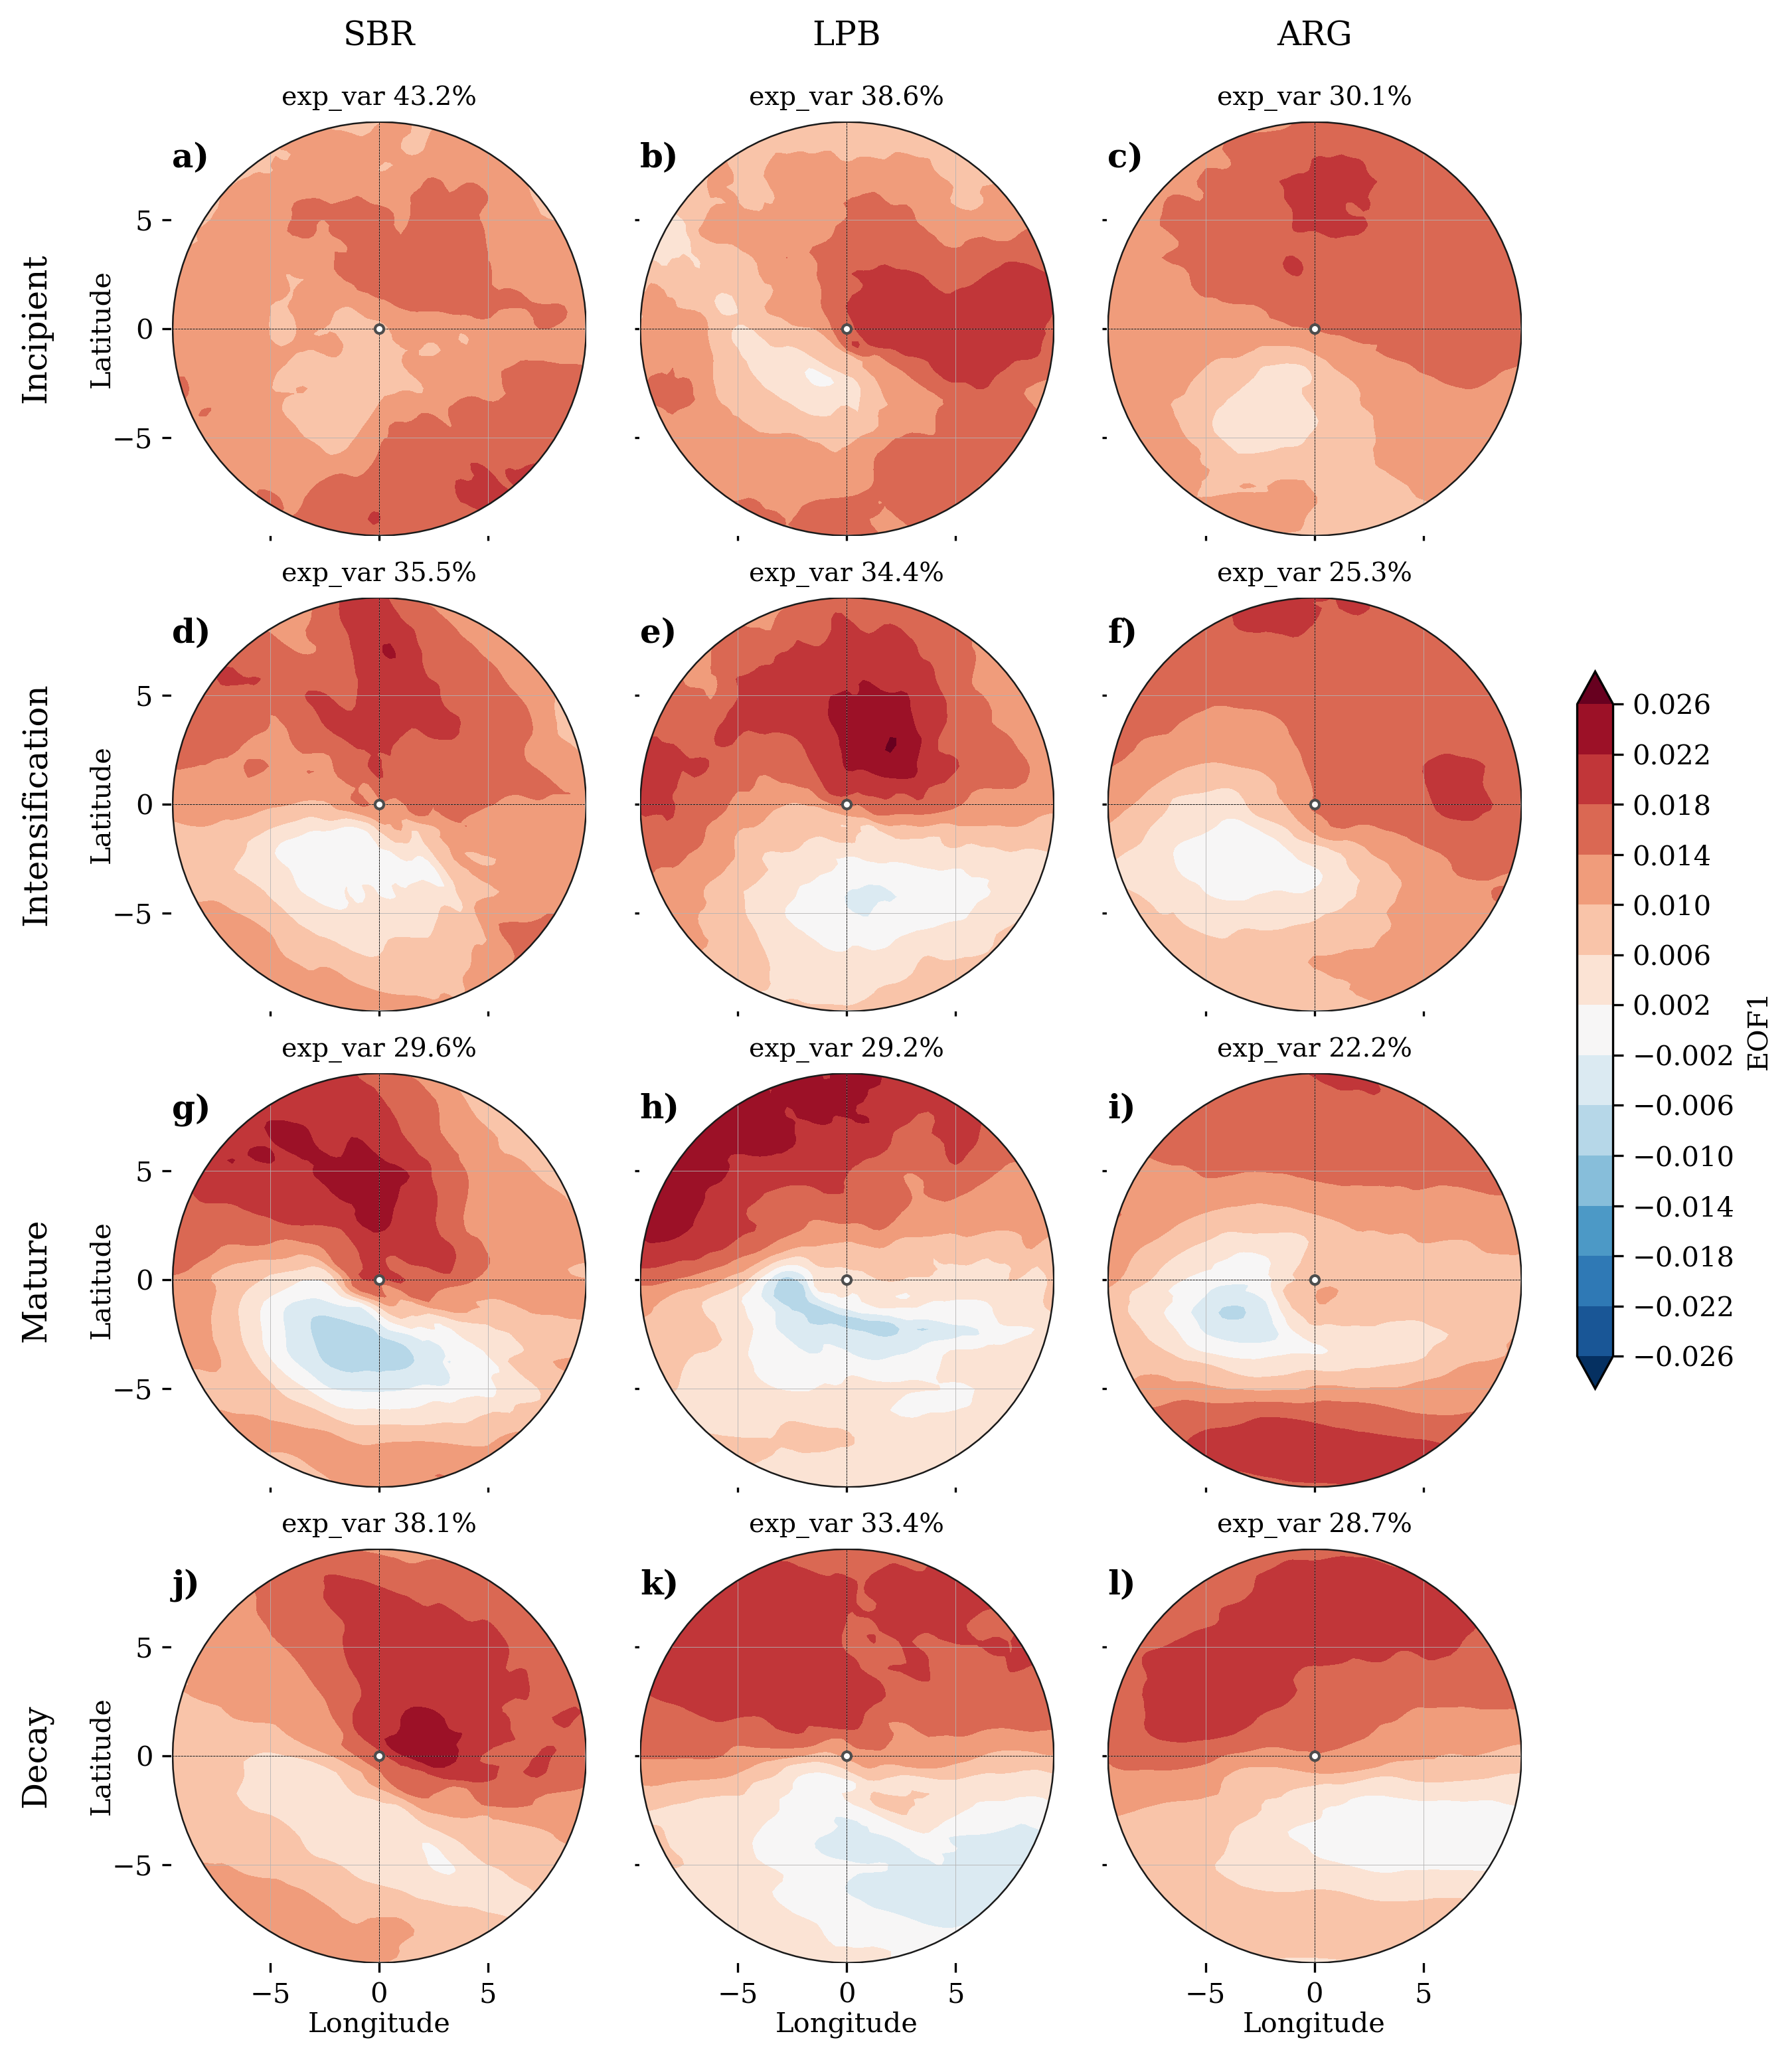
\includegraphics[width=\textwidth]{images/w100/pca1_wind100_p50_fasesxreg.png}
% \caption[EOF1 de viento a 100 m - Subconjunto p50]{Primer modo espacial (EOF1) de la magnitud del viento a 100 metros para el estrato de ciclones moderados (percentil 50). La varianza explicada oscila entre el $22.2\%$ y el $43.2\%$. El patrón representa el grado intermedio de organización estructural, donde el flujo de fondo comienza a verse distorsionado por la rotación interna del ciclón promedio, aunque sin alcanzar la alta concentración de los eventos severos.}
% \label{fig:eof1_wind100_p50_ap}
% \end{figure}

%

\section{Precipitação total (EOF)}\label{apendice:eof_tp}

\subsection{Sistemas fracos (p10)}\label{apendice:eof1_tp_p10}
\begin{figure}[htbp]
\centering
\includegraphics[width=\textwidth]{images/tp/pca1_tp_p10_fasesxreg.png}
\caption[EOF1 de precipitação total - Subconjunto p10]{Primeiro modo espacial (EOF1) da precipitação total para o estrato de ciclones fracos (percentil 10). A variância explicada oscila entre $9.2\%$ e $17.2\%$. O padrão retém a banda sudeste, porém de forma fragmentada e amorfa, confirmando que a carência de forçamento dinâmico profundo impede a organização estrutural da convecção em grande escala.}
\label{fig:eof1_tp_p10_ap}
\end{figure}

\subsection{Sistemas moderados (p50)}\label{apendice:eof1_tp_p50}
\begin{figure}[htbp]
\centering
\includegraphics[width=\textwidth]{images/tp/pca1_tp_p50_fasesxreg.png}
\caption[EOF1 de precipitação total - Subconjunto p50]{Primeiro modo espacial (EOF1) da precipitação total para o estrato de ciclones moderados (percentil 50). A variância explicada se consolida entre $9.7\%$ e $18.4\%$. Esse estrato reflete uma banda frontal sudeste muito mais definida que a do p10, operando como o passo intermediário de organização estrutural antes do severo enrolamento (\textit{wrap-around}) que caracteriza os eventos extremos do p90.}
\label{fig:eof1_tp_p50_ap}
\end{figure}
%%%%%%%%%%%%%%
% ==============================================================================
% ==============================================================================
% ==============================================================================
% XEOF MULTIDIMENSIONAL - APÉNDICE
% ==============================================================================

\chapter{Análise Multidimensional do Vento a 10 metros: Fases Evolutivas Adicionais}\label{apendice:xeof_fases}

Este apêndice complementa a análise multidimensional apresentada na seção de resultados. A seguir, documentam-se os padrões espaciais (EOF1, EOF2, EOF3) com suas respectivas zonas de significância estatística (calculadas mediante \textit{bootstrapping} com 15.000 iterações) e as PCs para as etapas incipiente, de intensificação e decaimento.

Contrastam-se os resultados da População Global de referência (climatologia geral) frente ao subconjunto de eventos dinamicamente extremos (percentil 90), permitindo observar a evolução temporal completa das assimetrias estruturais.

% ------------------------------------------------------------------------------
\section{População Global}
% ------------------------------------------------------------------------------

\begin{figure}[htbp]
\centering
\includegraphics[width=\textwidth]{images/w10/xeof_global_wind10_incipient.jpg}
\caption[EOF1-3  - Población Global (Incipiente)]{Análise multidimensional do vento a 10 metros para a \textbf{População Global} durante a \textbf{fase incipiente}. As zonas pontilhadas indicam significância estatística ao nível empírico de 95\%.}
\label{fig:apendice_global_incipiente}
\end{figure}

\begin{figure}[htbp]
\centering
\includegraphics[width=\textwidth]{images/w10/xeof_global_wind10_intensification.jpg}
\caption[EOF1-3  - Población Global (Intensificación)]{Análise multidimensional do vento a 10 metros para a \textbf{População Global} durante a \textbf{fase de intensificação}. As zonas pontilhadas indicam significância estatística ao nível empírico de 95\%.}
\label{fig:apendice_global_intensificacion}
\end{figure}

\begin{figure}[htbp]
\centering
\includegraphics[width=\textwidth]{images/w10/xeof_global_wind10_decay.jpg}
\caption[EOF1-3  - Población Global (Decaimiento)]{Análise multidimensional do vento a 10 metros para a \textbf{População Global} durante a \textbf{fase de decaimento}. As zonas pontilhadas indicam significância estatística ao nível empírico de 95\%.}
\label{fig:apendice_global_decaimiento}
\end{figure}

\clearpage

% ------------------------------------------------------------------------------
\section{Subconjunto Extremo (p90)}
% ------------------------------------------------------------------------------

\begin{figure}[htbp]
\centering
\includegraphics[width=\textwidth]{images/w10/xeof_p90_wind10_incipient.jpg}
\caption[EOF1-3  - Subconjunto p90 (Incipiente)]{Análise multidimensional do vento a 10 metros para o \textbf{subconjunto extremo (p90)} durante a \textbf{fase incipiente}. As zonas pontilhadas indicam significância estatística ao nível empírico de 95\%, evidenciando alterações precoces em relação à população global.}
\label{fig:apendice_p90_incipiente}
\end{figure}

\begin{figure}[htbp]
\centering
\includegraphics[width=\textwidth]{images/w10/xeof_p90_wind10_intensification.jpg}
\caption[EOF1-3  - Subconjunto p90 (Intensificación)]{Análise multidimensional do vento a 10 metros para o \textbf{subconjunto extremo (p90)} durante a \textbf{fase de intensificação}. As zonas pontilhadas indicam significância estatística ao nível empírico de 95\%.}
\label{fig:apendice_p90_intensificacion}
\end{figure}

\begin{figure}[htbp]
\centering
\includegraphics[width=\textwidth]{images/w10/xeof_p90_wind10_decay.jpg}
\caption[EOF1-3  - Subconjunto p90 (Decaimiento)]{Análise multidimensional do vento a 10 metros para o \textbf{subconjunto extremo (p90)} durante a \textbf{fase de decaimento}. As zonas pontilhadas indicam significância estatística ao nível empírico de 95\%.}
\label{fig:apendice_p90_decaimiento}
\end{figure}
% ==============================================================================
% ==============================================================================
% ==============================================================================
\chapter{Análise Multivariada Complementar (MEOF)}\label{apendice:meof}

% ==============================================================================
% FASE INCIPIENTE
% ==============================================================================
\section{Fase Incipiente: Vento a 100 metros e Precipitação (p10 e p50)}\label{apendice:meof_incipiente}

\begin{figure}[htbp]
\centering
\includegraphics[width=\textwidth]{images/meof/meof1_incipient_p10.png}
\caption[MEOF1 de viento a 100 m y precipitación (Incipiente) - p10]{Primeiro modo espacial multivariado (MEOF1) durante a fase incipiente para o estrato de baixa intensidade dinâmica (p10). A matriz organiza os resultados em colunas por região de ciclogênese (SBR, LPB e ARG) e em linhas pareadas (a linha superior expõe a anomalia de precipitação e a inferior seu padrão covariante de vento a 100 metros). Com uma variância explicada entre $12.7\%$ e $13.6\%$, a falta de covariância espacial estruturada é quase absoluta, refletindo o ruído espacial de sistemas que carecem de um forçamento inicial profundo.}
\label{fig:meof_incipiente_p10_ap}
\end{figure}

\begin{figure}[htbp]
\centering
\includegraphics[width=\textwidth]{images/meof/meof1_incipient_p50.png}
\caption[MEOF1 de viento a 100 m y precipitación (Incipiente) - p50]{Primeiro modo espacial multivariado (MEOF1) durante a fase incipiente para o estrato de intensidade moderada (p50). Mantendo a mesma disposição geométrica de linhas pareadas, esse grupo (variância entre $14.3\%$ e $19.1\%$) mostra os primeiros indícios sutis de alinhamento frontal entre ambas as variáveis, servindo como a linha de base ideal para dimensionar a organização precoce agressiva alcançada pelos eventos severos (p90).}
\label{fig:meof_incipiente_p50_ap}
\end{figure}

% ==============================================================================
% FASE DE INTENSIFICACIÓN
% ==============================================================================
\section{Fase de Intensificação: Vento a 100 metros e Precipitação (p10 e p50)}\label{apendice:meof_intensificacion}

\begin{figure}[htbp]
\centering
\includegraphics[width=\textwidth]{images/meof/meof1_intensification_p10.png}
\caption[MEOF1 de viento a 100 m y precipitación (Intensificación) - p10]{Primeiro modo espacial multivariado (MEOF1) durante a fase de Intensificação para o estrato p10. Ao avaliar as linhas pareadas de precipitação e vento, observa-se que o sistema retém uma covariância extremamente difusa (variância $\sim 13.8\%-15.1\%$), evidenciando sua incapacidade termodinâmica de organizar gradientes anômalos durante sua etapa de aprofundamento.}
\label{fig:meof_intensificacion_p10_ap}
\end{figure}

\begin{figure}[htbp]
\centering
\includegraphics[width=\textwidth]{images/meof/meof1_intensification_p50.png}
\caption[MEOF1 de viento a 100 m y precipitación (Intensificación) - p50]{Primeiro modo espacial multivariado (MEOF1) durante a fase de Intensificação para o estrato p50. Esse grupo apresenta uma variância conjunta de $11.5\%$ a $15.6\%$ e funciona como um degrau de transição estrutural: as linhas pareadas começam a mostrar maior superposição em seus sinais, mas sem jamais alcançar a concentração assimétrica violenta dos gradientes que distingue o estrato extremo (p90).}
\label{fig:meof_intensificacion_p50_ap}
\end{figure}

% ==============================================================================
% FASE DE MADUREZ
% ==============================================================================
\section{Fase de Maturidade: Vento a 100 metros e Precipitação (p10 e p50)}\label{apendice:meof_madurez}

\begin{figure}[htbp]
\centering
\includegraphics[width=\textwidth]{images/meof/meof1_mature_p10.png}
\caption[MEOF1 de viento a 100 m y precipitación (Madurez) - p10]{Primeiro modo espacial multivariado (MEOF1) durante a fase de Maturidade para o estrato p10, organizado em colunas (SBR, LPB, ARG) e linhas pareadas. Mesmo no momento de sua máxima (embora fraca) vorticidade, o grupo mantém uma covariabilidade dispersa e espacialmente ruidosa, capturando uma variância conjunta marginal (entre $14.3\%$ e $15.0\%$).}
\label{fig:meof_madurez_p10_ap}
\end{figure}

\begin{figure}[htbp]
\centering
\includegraphics[width=\textwidth]{images/meof/meof1_mature_p50.png}
\caption[MEOF1 de viento a 100 m y precipitación (Madurez) - p50]{Primeiro modo espacial multivariado (MEOF1) durante a fase de Maturidade para o estrato p50. Com uma variância explicada de $10.7\%$ a $15.8\%$, o sistema consegue delinear as bandas frontais básicas de chuva e vento. No entanto, sua superposição geográfica linear é análoga ao comportamento da População Global, carecendo da expulsão periférica violenta de umidade (separação topológica) produzida pelo forçamento extremo dos sistemas p90.}
\label{fig:meof_madurez_p50_ap}
\end{figure}

% ==============================================================================
% FASE DE DECAIMIENTO
% ==============================================================================
\section{Fase de Decaimento: Vento a 100 metros e Precipitação (p10 e p50)}\label{apendice:meof_decaimiento}

\begin{figure}[htbp]
\centering
\includegraphics[width=\textwidth]{images/meof/meof1_decay_p10.png}
\caption[MEOF1 de viento a 100 m y precipitación (Decaimiento) - p10]{Primeiro modo espacial multivariado (MEOF1) durante a fase de Decaimento para o estrato p10. Avaliado sob o formato de matrizes pareadas, os mapas mostram a desorganização progressiva em direção ao ruído ambiental tanto no campo pluviométrico quanto no cinemático, estabilizando-se a variância conjunta entre $16.1\%$ e $17.6\%$.}
\label{fig:meof_decaimiento_p10_ap}
\end{figure}

\begin{figure}[htbp]
\centering
\includegraphics[width=\textwidth]{images/meof/meof1_decay_p50.png}
\caption[MEOF1 de viento a 100 m y precipitación (Decaimiento) - p50]{Primeiro modo espacial multivariado (MEOF1) durante a fase de Decaimento para o estrato p50. Exibe um padrão de dissipação covariante suave (variância entre $14.4\%$ e $19.1\%$), replicando o relaxamento homogêneo e a perda conjunta de gradientes que caracteriza os sistemas ordinários ao esgotar seu forçamento dinâmico e finalizar seu ciclo de vida.}
\label{fig:meof_decaimiento_p50_ap}
\end{figure}

% ==============================================================================
% VERIFICACIÓN DEL SESGO DE BRETHERTON (MEOF VS. EOF UNIVARIADO)
% ==============================================================================
\section{Verificação do viés para um único campo (Bretherton et al., 1992)}\label{apendice:meof_bias}

Esta seção complementa a discussão do Capítulo~\ref{chap:meof} sobre o risco, apontado por \citet{bretherton1992intercomparison}, de que o MEOF se incline para o EOF dominante de um único campo. A Tabela~\ref{tab:meof_bias_check_completa} apresenta a correlação espacial (em valor absoluto) entre a carga de cada campo dentro do MEOF1 e o padrão de seu próprio EOF1 univariado, para as quatro fases do ciclo de vida, complementando a Tabela~\ref{tab:meof_bias_check} do corpo do capítulo (que apresenta apenas incipiente e maturidade).

\begin{table}[htbp]
\centering
\caption[Correlação espacial entre o MEOF1 e os EOF1 univariados (as quatro fases)]{Correlação espacial (valor absoluto, $|r|$) entre a carga de cada campo dentro do MEOF1 e o padrão de seu próprio EOF1 univariado (vento a 10 m; precipitação), para a População Global e o subconjunto p90, nas quatro fases do ciclo de vida.}
\label{tab:meof_bias_check_completa}
\begin{tabular*}{\textwidth}{@{\extracolsep{\fill}}llrrrr}
\hline
\textbf{Região} & \textbf{Fase} & \multicolumn{2}{c}{\textbf{População Global}} & \multicolumn{2}{c}{\textbf{Subconjunto p90}} \\
\cline{3-4} \cline{5-6}
 & & \textbf{$|r|$ vento} & \textbf{$|r|$ precip.} & \textbf{$|r|$ vento} & \textbf{$|r|$ precip.} \\
\hline
\textbf{SBR} & Incipiente & 0.99 & 0.83 & 0.99 & 0.74 \\
 & Intensificação & 1.00 & 0.72 & 0.96 & 0.20 \\
 & Maturidade & 1.00 & 0.55 & 0.99 & 0.94 \\
 & Decaimento & 1.00 & 0.81 & 0.26 & 0.99 \\
\hline
\textbf{LPB} & Incipiente & 0.99 & 0.94 & 0.99 & 0.25 \\
 & Intensificação & 1.00 & 0.84 & 1.00 & 0.08 \\
 & Maturidade & 1.00 & 0.33 & 0.94 & 0.97 \\
 & Decaimento & 1.00 & 0.37 & 0.71 & 1.00 \\
\hline
\textbf{ARG} & Incipiente & 1.00 & 0.56 & 1.00 & 0.49 \\
 & Intensificação & 0.99 & 0.95 & 0.97 & 0.92 \\
 & Maturidade & 0.99 & 0.79 & 0.94 & 0.97 \\
 & Decaimento & 1.00 & 0.49 & 0.84 & 0.85 \\
\hline
\end{tabular*}
\end{table}


		% apendice anterior (no incluido)
% ==============================================================================
% APÊNDICE. VERIFICAÇÃO DO VIÉS DE BRETHERTON (MEOF VS. EOF UNIVARIADO)
% ==============================================================================
\chapter{Verificação do viés do MEOF em direção a um único campo}\label{apendice:meof_bias}

Este apêndice complementa a discussão do Capítulo~\ref{chap:meof} sobre o risco, apontado por \citet{bretherton1992intercomparison}, de que o MEOF se enviese em direção ao EOF dominante de um único campo. A Tabela~\ref{tab:meof_bias_check_completa} apresenta a correlação espacial (em valor absoluto) entre a carga de cada campo dentro do MEOF1 e o padrão de seu próprio EOF1 univariado, para as quatro fases do ciclo de vida. A Tabela~\ref{tab:meof_bias_check} do Capítulo~\ref{chap:meof} apresenta apenas as fases incipiente e maturidade.

\begin{table}[htbp]
\centering
\caption[Correlação espacial entre o MEOF1 e os EOF1 univariados (as quatro fases)]{Correlação espacial (valor absoluto, $|r|$) entre a carga de cada campo dentro do MEOF1 e o padrão de seu próprio EOF1 univariado (vento a 10 m; precipitação), para a População Global e o subconjunto p90, nas quatro fases do ciclo de vida.}
\label{tab:meof_bias_check_completa}
\begin{tabular*}{\textwidth}{@{\extracolsep{\fill}}llrrrr}
\hline
\textbf{Região} & \textbf{Fase} & \multicolumn{2}{c}{\textbf{População Global}} & \multicolumn{2}{c}{\textbf{Subconjunto p90}} \\
\cline{3-4} \cline{5-6}
 & & \textbf{$|r|$ vento} & \textbf{$|r|$ precip.} & \textbf{$|r|$ vento} & \textbf{$|r|$ precip.} \\
\hline
\textbf{SBR} & Incipiente & 0.99 & 0.83 & 0.99 & 0.74 \\
 & Intensificação & 1.00 & 0.72 & 0.96 & 0.20 \\
 & Maturidade & 1.00 & 0.55 & 0.99 & 0.94 \\
 & Decaimento & 1.00 & 0.81 & 0.26 & 0.99 \\
\hline
\textbf{LPB} & Incipiente & 0.99 & 0.94 & 0.99 & 0.25 \\
 & Intensificação & 1.00 & 0.84 & 1.00 & 0.08 \\
 & Maturidade & 1.00 & 0.33 & 0.94 & 0.97 \\
 & Decaimento & 1.00 & 0.37 & 0.71 & 1.00 \\
\hline
\textbf{ARG} & Incipiente & 1.00 & 0.56 & 1.00 & 0.49 \\
 & Intensificação & 0.99 & 0.95 & 0.97 & 0.92 \\
 & Maturidade & 0.99 & 0.79 & 0.94 & 0.97 \\
 & Decaimento & 1.00 & 0.49 & 0.84 & 0.85 \\
\hline
\end{tabular*}
\end{table}

	% verificacao do viés MEOF (Bretherton)
\end{apendice}				% fim do ambiente apendice. caso
						% nao utilize apendice, remova as
						% 3 linhas de comando.
						%
\end{document}				% fim do arquivo